\documentclass[ngerman, aspectratio=169, xcolor={rgb}]{beamer}

% style
\mode<presentation>{
	\usetheme{Frankfurt}
}
%packages
\usepackage[utf8]{inputenc}\DeclareUnicodeCharacter{2212}{-}
\usepackage[english]{babel}
\usepackage{graphicx}
\usepackage{array}

\newcolumntype{L}[1]{>{\raggedright\let\newline\\\arraybackslash\hspace{0pt}}m{#1}}
\usepackage{ragged2e}

\usepackage{bm} % bold math
\usepackage{amsfonts}
\usepackage{amssymb}
\usepackage{mathtools}
\usepackage{amsmath}
\usepackage{multirow} % multi row in tables
\usepackage{booktabs} %toprule midrule bottomrue in tables
\usepackage{scrextend}
\usepackage{textgreek}
\usepackage[rgb]{xcolor}

\usepackage{ marvosym } % \Lightning

\usepackage{multimedia} % embedded videos

\usepackage{tikz}
\usepackage{pgf}
\usepackage{pgfplots}

\usepackage{algorithmic}

%citations
\usepackage[style=verbose,backend=biber]{biblatex}
\addbibresource{references.bib}


%math font
\usefonttheme[onlymath]{serif}

%Beamer Template modifications
%\definecolor{mainColor}{HTML}{0065A3} % HSR blue
\definecolor{mainColor}{HTML}{D72864} % OST pink
\definecolor{invColor}{HTML}{28d79b} % OST pink
\definecolor{dgreen}{HTML}{38ad36} % Dark green

%\definecolor{mainColor}{HTML}{000000} % HSR blue
\setbeamercolor{palette primary}{bg=white,fg=mainColor}
\setbeamercolor{palette secondary}{bg=orange,fg=mainColor}
\setbeamercolor{palette tertiary}{bg=yellow,fg=red}
\setbeamercolor{palette quaternary}{bg=mainColor,fg=white} %bg = Top bar, fg = active top bar topic
\setbeamercolor{structure}{fg=black} % itemize, enumerate, etc (bullet points)
\setbeamercolor{section in toc}{fg=black} % TOC sections
\setbeamertemplate{section in toc}[sections numbered]
\setbeamertemplate{subsection in toc}{%
	\hspace{1.2em}{$\bullet$}~\inserttocsubsection\par}

\setbeamertemplate{itemize items}[circle]
\setbeamertemplate{description item}[circle]
\setbeamertemplate{title page}[default][colsep=-4bp,rounded=true]
\beamertemplatenavigationsymbolsempty

\setbeamercolor{footline}{fg=gray}
\setbeamertemplate{footline}{%
	\hfill\usebeamertemplate***{navigation symbols}
	\hspace{0.5cm}
	\insertframenumber{}\hspace{0.2cm}\vspace{0.2cm}
}

\usepackage{caption}
\captionsetup{labelformat=empty}

%Title Page
\title{Elliptische Filter}
\subtitle{Eine Anwendung der Jacobi elliptischen Funktionen}
\author{Nicolas Tobler}
\institute{Mathematisches Seminar 2022 | Spezielle Funktionen}
% \institute{\includegraphics[scale=0.3]{../img/ost_logo.png}}
\date{\today}

%
% packages.tex -- packages required by the paper kugel
%
% (c) 2019 Prof Dr Andreas Müller, Hochschule Rapperswil
%

% if your paper needs special packages, add package commands as in the
% following example
%\usepackage{packagename}
\usepackage{cases}

\newcommand{\kugeltodo}[1]{\textcolor{red!70!black}{\texttt{[TODO: #1]}}}

\DeclareMathOperator{\sphlaplacian}{\nabla^2_{\mathit{S}}}
\DeclareMathOperator{\surflaplacian}{\nabla^2_{\partial \mathit{S}}}


\newcommand*{\QED}{\hfill\ensuremath{\blacksquare}}%

\newcommand*{\HL}{\textcolor{mainColor}}
\newcommand*{\RD}{\textcolor{red}}
\newcommand*{\BL}{\textcolor{blue}}
\newcommand*{\GN}{\textcolor{dgreen}}

\definecolor{darkgreen}{rgb}{0,0.6,0}


\makeatletter
\newcount\my@repeat@count
\newcommand{\myrepeat}[2]{%
	\begingroup
	\my@repeat@count=\z@
	\@whilenum\my@repeat@count<#1\do{#2\advance\my@repeat@count\@ne}%
	\endgroup
}
\makeatother

\usetikzlibrary{automata,arrows,positioning,calc,shapes.geometric, fadings}

\begin{document}

	\begin{frame}
		\titlepage
	\end{frame}

	\begin{frame}
		\frametitle{Inhalt}
		\tableofcontents
	\end{frame}

	\section{Lineare Filter}

	\begin{frame}
		\frametitle{Lineare Filter}

		\begin{center}
			\scalebox{0.75}{
				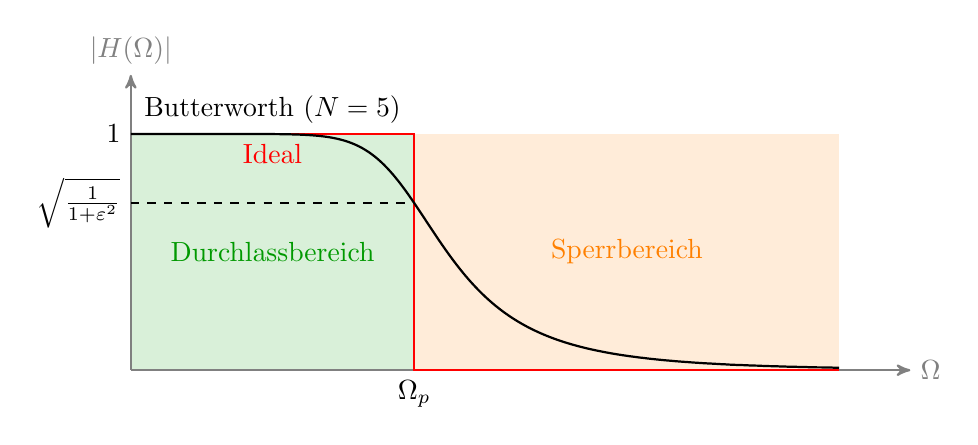
\begin{tikzpicture}[>=stealth', auto, node distance=2cm, scale=1.2, thick]

    \tikzstyle{zero} = [draw, circle, inner sep =0, minimum height=0.15cm]

    \tikzset{pole/.style={cross out, draw=black, minimum size=(0.15cm-\pgflinewidth), inner sep=0pt, outer sep=0pt}}

    \begin{scope}[xscale=3, yscale=2.5]

        \fill[darkgreen!15] (0,0) rectangle  (1,1);
        \node[darkgreen] at (0.5,0.5) {Durchlassbereich};
        \fill[orange!15] (1,0) rectangle  (2.5,1);
        \node[orange] at (1.75,0.5) {Sperrbereich};

        \draw[gray, ->] (0,0) -- (0,1.25) node[anchor=south]{$|H(\Omega)|$};
        \draw[gray, ->] (0,0) -- (2.75,0) node[anchor=west]{$\Omega$};

        \draw[dashed] (0,0.707) node[left] {$\sqrt{\frac{1}{1+\varepsilon^2}}$} -- (1, 0.707) (1,0) node[below] {$\Omega_p$};

        \node[left] at(0,1) {$1$};

        \draw[red, thick] (0,1) -- (1,1) -- (1,0) -- (2.5,0);

        \node[anchor=north, red] at (0.5,1) {Ideal};

        \draw[thick, domain=0:2.5,  variable=\x, smooth, samples=200] plot
        ({\x}, {sqrt(abs(1/ (1 + \x^10)))});
        \node[anchor=south] at (0.5,1) {Butterworth ($N=5$)};

    \end{scope}

\end{tikzpicture}

			}
		\end{center}


		\begin{equation*}
			| H(\Omega)|^2 = \frac{1}{1 + \varepsilon_p^2 F_N^2(w)}, \quad w=\frac{\Omega}{\Omega_p}
		\end{equation*}

		\pause

		\begin{align*}
			|F_N(w)| &< 1 \quad \forall \quad |w| < 1 \\
			|F_N(w)| &= 1 \quad \forall \quad |w| = 1 \\
			|F_N(w)| &> 1 \quad \forall \quad |w| > 1
		\end{align*}


		\begin{equation*}
			F_N(w) = w^N
		\end{equation*}

	\end{frame}

	\begin{frame}
		\frametitle{Beispiel: Butterworth Filter}

		\begin{equation}
			F_N(w) = w^N
		\end{equation}

		\begin{center}
			%% Creator: Matplotlib, PGF backend
%%
%% To include the figure in your LaTeX document, write
%%   \input{<filename>.pgf}
%%
%% Make sure the required packages are loaded in your preamble
%%   \usepackage{pgf}
%%
%% Also ensure that all the required font packages are loaded; for instance,
%% the lmodern package is sometimes necessary when using math font.
%%   \usepackage{lmodern}
%%
%% Figures using additional raster images can only be included by \input if
%% they are in the same directory as the main LaTeX file. For loading figures
%% from other directories you can use the `import` package
%%   \usepackage{import}
%%
%% and then include the figures with
%%   \import{<path to file>}{<filename>.pgf}
%%
%% Matplotlib used the following preamble
%%
\begingroup%
\makeatletter%
\begin{pgfpicture}%
\pgfpathrectangle{\pgfpointorigin}{\pgfqpoint{4.000000in}{2.500000in}}%
\pgfusepath{use as bounding box, clip}%
\begin{pgfscope}%
\pgfsetbuttcap%
\pgfsetmiterjoin%
\pgfsetlinewidth{0.000000pt}%
\definecolor{currentstroke}{rgb}{1.000000,1.000000,1.000000}%
\pgfsetstrokecolor{currentstroke}%
\pgfsetstrokeopacity{0.000000}%
\pgfsetdash{}{0pt}%
\pgfpathmoveto{\pgfqpoint{0.000000in}{0.000000in}}%
\pgfpathlineto{\pgfqpoint{4.000000in}{0.000000in}}%
\pgfpathlineto{\pgfqpoint{4.000000in}{2.500000in}}%
\pgfpathlineto{\pgfqpoint{0.000000in}{2.500000in}}%
\pgfpathlineto{\pgfqpoint{0.000000in}{0.000000in}}%
\pgfpathclose%
\pgfusepath{}%
\end{pgfscope}%
\begin{pgfscope}%
\pgfsetbuttcap%
\pgfsetmiterjoin%
\definecolor{currentfill}{rgb}{1.000000,1.000000,1.000000}%
\pgfsetfillcolor{currentfill}%
\pgfsetlinewidth{0.000000pt}%
\definecolor{currentstroke}{rgb}{0.000000,0.000000,0.000000}%
\pgfsetstrokecolor{currentstroke}%
\pgfsetstrokeopacity{0.000000}%
\pgfsetdash{}{0pt}%
\pgfpathmoveto{\pgfqpoint{0.630330in}{0.548769in}}%
\pgfpathlineto{\pgfqpoint{3.727004in}{0.548769in}}%
\pgfpathlineto{\pgfqpoint{3.727004in}{2.301955in}}%
\pgfpathlineto{\pgfqpoint{0.630330in}{2.301955in}}%
\pgfpathlineto{\pgfqpoint{0.630330in}{0.548769in}}%
\pgfpathclose%
\pgfusepath{fill}%
\end{pgfscope}%
\begin{pgfscope}%
\pgfpathrectangle{\pgfqpoint{0.630330in}{0.548769in}}{\pgfqpoint{3.096674in}{1.753186in}}%
\pgfusepath{clip}%
\pgfsetbuttcap%
\pgfsetmiterjoin%
\definecolor{currentfill}{rgb}{0.000000,0.501961,0.000000}%
\pgfsetfillcolor{currentfill}%
\pgfsetfillopacity{0.200000}%
\pgfsetlinewidth{0.000000pt}%
\definecolor{currentstroke}{rgb}{0.000000,0.000000,0.000000}%
\pgfsetstrokecolor{currentstroke}%
\pgfsetstrokeopacity{0.200000}%
\pgfsetdash{}{0pt}%
\pgfpathmoveto{\pgfqpoint{0.630330in}{0.548769in}}%
\pgfpathlineto{\pgfqpoint{2.694779in}{0.548769in}}%
\pgfpathlineto{\pgfqpoint{2.694779in}{1.425362in}}%
\pgfpathlineto{\pgfqpoint{0.630330in}{1.425362in}}%
\pgfpathlineto{\pgfqpoint{0.630330in}{0.548769in}}%
\pgfpathclose%
\pgfusepath{fill}%
\end{pgfscope}%
\begin{pgfscope}%
\pgfpathrectangle{\pgfqpoint{0.630330in}{0.548769in}}{\pgfqpoint{3.096674in}{1.753186in}}%
\pgfusepath{clip}%
\pgfsetbuttcap%
\pgfsetmiterjoin%
\definecolor{currentfill}{rgb}{1.000000,0.647059,0.000000}%
\pgfsetfillcolor{currentfill}%
\pgfsetfillopacity{0.200000}%
\pgfsetlinewidth{0.000000pt}%
\definecolor{currentstroke}{rgb}{0.000000,0.000000,0.000000}%
\pgfsetstrokecolor{currentstroke}%
\pgfsetstrokeopacity{0.200000}%
\pgfsetdash{}{0pt}%
\pgfpathmoveto{\pgfqpoint{2.694779in}{1.425362in}}%
\pgfpathlineto{\pgfqpoint{3.727004in}{1.425362in}}%
\pgfpathlineto{\pgfqpoint{3.727004in}{2.301955in}}%
\pgfpathlineto{\pgfqpoint{2.694779in}{2.301955in}}%
\pgfpathlineto{\pgfqpoint{2.694779in}{1.425362in}}%
\pgfpathclose%
\pgfusepath{fill}%
\end{pgfscope}%
\begin{pgfscope}%
\pgfpathrectangle{\pgfqpoint{0.630330in}{0.548769in}}{\pgfqpoint{3.096674in}{1.753186in}}%
\pgfusepath{clip}%
\pgfsetrectcap%
\pgfsetroundjoin%
\pgfsetlinewidth{0.803000pt}%
\definecolor{currentstroke}{rgb}{0.690196,0.690196,0.690196}%
\pgfsetstrokecolor{currentstroke}%
\pgfsetdash{}{0pt}%
\pgfpathmoveto{\pgfqpoint{0.630330in}{0.548769in}}%
\pgfpathlineto{\pgfqpoint{0.630330in}{2.301955in}}%
\pgfusepath{stroke}%
\end{pgfscope}%
\begin{pgfscope}%
\pgfsetbuttcap%
\pgfsetroundjoin%
\definecolor{currentfill}{rgb}{0.000000,0.000000,0.000000}%
\pgfsetfillcolor{currentfill}%
\pgfsetlinewidth{0.803000pt}%
\definecolor{currentstroke}{rgb}{0.000000,0.000000,0.000000}%
\pgfsetstrokecolor{currentstroke}%
\pgfsetdash{}{0pt}%
\pgfsys@defobject{currentmarker}{\pgfqpoint{0.000000in}{-0.048611in}}{\pgfqpoint{0.000000in}{0.000000in}}{%
\pgfpathmoveto{\pgfqpoint{0.000000in}{0.000000in}}%
\pgfpathlineto{\pgfqpoint{0.000000in}{-0.048611in}}%
\pgfusepath{stroke,fill}%
}%
\begin{pgfscope}%
\pgfsys@transformshift{0.630330in}{0.548769in}%
\pgfsys@useobject{currentmarker}{}%
\end{pgfscope}%
\end{pgfscope}%
\begin{pgfscope}%
\definecolor{textcolor}{rgb}{0.000000,0.000000,0.000000}%
\pgfsetstrokecolor{textcolor}%
\pgfsetfillcolor{textcolor}%
\pgftext[x=0.630330in,y=0.451547in,,top]{\color{textcolor}\rmfamily\fontsize{10.000000}{12.000000}\selectfont \(\displaystyle {0.00}\)}%
\end{pgfscope}%
\begin{pgfscope}%
\pgfpathrectangle{\pgfqpoint{0.630330in}{0.548769in}}{\pgfqpoint{3.096674in}{1.753186in}}%
\pgfusepath{clip}%
\pgfsetrectcap%
\pgfsetroundjoin%
\pgfsetlinewidth{0.803000pt}%
\definecolor{currentstroke}{rgb}{0.690196,0.690196,0.690196}%
\pgfsetstrokecolor{currentstroke}%
\pgfsetdash{}{0pt}%
\pgfpathmoveto{\pgfqpoint{1.146442in}{0.548769in}}%
\pgfpathlineto{\pgfqpoint{1.146442in}{2.301955in}}%
\pgfusepath{stroke}%
\end{pgfscope}%
\begin{pgfscope}%
\pgfsetbuttcap%
\pgfsetroundjoin%
\definecolor{currentfill}{rgb}{0.000000,0.000000,0.000000}%
\pgfsetfillcolor{currentfill}%
\pgfsetlinewidth{0.803000pt}%
\definecolor{currentstroke}{rgb}{0.000000,0.000000,0.000000}%
\pgfsetstrokecolor{currentstroke}%
\pgfsetdash{}{0pt}%
\pgfsys@defobject{currentmarker}{\pgfqpoint{0.000000in}{-0.048611in}}{\pgfqpoint{0.000000in}{0.000000in}}{%
\pgfpathmoveto{\pgfqpoint{0.000000in}{0.000000in}}%
\pgfpathlineto{\pgfqpoint{0.000000in}{-0.048611in}}%
\pgfusepath{stroke,fill}%
}%
\begin{pgfscope}%
\pgfsys@transformshift{1.146442in}{0.548769in}%
\pgfsys@useobject{currentmarker}{}%
\end{pgfscope}%
\end{pgfscope}%
\begin{pgfscope}%
\definecolor{textcolor}{rgb}{0.000000,0.000000,0.000000}%
\pgfsetstrokecolor{textcolor}%
\pgfsetfillcolor{textcolor}%
\pgftext[x=1.146442in,y=0.451547in,,top]{\color{textcolor}\rmfamily\fontsize{10.000000}{12.000000}\selectfont \(\displaystyle {0.25}\)}%
\end{pgfscope}%
\begin{pgfscope}%
\pgfpathrectangle{\pgfqpoint{0.630330in}{0.548769in}}{\pgfqpoint{3.096674in}{1.753186in}}%
\pgfusepath{clip}%
\pgfsetrectcap%
\pgfsetroundjoin%
\pgfsetlinewidth{0.803000pt}%
\definecolor{currentstroke}{rgb}{0.690196,0.690196,0.690196}%
\pgfsetstrokecolor{currentstroke}%
\pgfsetdash{}{0pt}%
\pgfpathmoveto{\pgfqpoint{1.662555in}{0.548769in}}%
\pgfpathlineto{\pgfqpoint{1.662555in}{2.301955in}}%
\pgfusepath{stroke}%
\end{pgfscope}%
\begin{pgfscope}%
\pgfsetbuttcap%
\pgfsetroundjoin%
\definecolor{currentfill}{rgb}{0.000000,0.000000,0.000000}%
\pgfsetfillcolor{currentfill}%
\pgfsetlinewidth{0.803000pt}%
\definecolor{currentstroke}{rgb}{0.000000,0.000000,0.000000}%
\pgfsetstrokecolor{currentstroke}%
\pgfsetdash{}{0pt}%
\pgfsys@defobject{currentmarker}{\pgfqpoint{0.000000in}{-0.048611in}}{\pgfqpoint{0.000000in}{0.000000in}}{%
\pgfpathmoveto{\pgfqpoint{0.000000in}{0.000000in}}%
\pgfpathlineto{\pgfqpoint{0.000000in}{-0.048611in}}%
\pgfusepath{stroke,fill}%
}%
\begin{pgfscope}%
\pgfsys@transformshift{1.662555in}{0.548769in}%
\pgfsys@useobject{currentmarker}{}%
\end{pgfscope}%
\end{pgfscope}%
\begin{pgfscope}%
\definecolor{textcolor}{rgb}{0.000000,0.000000,0.000000}%
\pgfsetstrokecolor{textcolor}%
\pgfsetfillcolor{textcolor}%
\pgftext[x=1.662555in,y=0.451547in,,top]{\color{textcolor}\rmfamily\fontsize{10.000000}{12.000000}\selectfont \(\displaystyle {0.50}\)}%
\end{pgfscope}%
\begin{pgfscope}%
\pgfpathrectangle{\pgfqpoint{0.630330in}{0.548769in}}{\pgfqpoint{3.096674in}{1.753186in}}%
\pgfusepath{clip}%
\pgfsetrectcap%
\pgfsetroundjoin%
\pgfsetlinewidth{0.803000pt}%
\definecolor{currentstroke}{rgb}{0.690196,0.690196,0.690196}%
\pgfsetstrokecolor{currentstroke}%
\pgfsetdash{}{0pt}%
\pgfpathmoveto{\pgfqpoint{2.178667in}{0.548769in}}%
\pgfpathlineto{\pgfqpoint{2.178667in}{2.301955in}}%
\pgfusepath{stroke}%
\end{pgfscope}%
\begin{pgfscope}%
\pgfsetbuttcap%
\pgfsetroundjoin%
\definecolor{currentfill}{rgb}{0.000000,0.000000,0.000000}%
\pgfsetfillcolor{currentfill}%
\pgfsetlinewidth{0.803000pt}%
\definecolor{currentstroke}{rgb}{0.000000,0.000000,0.000000}%
\pgfsetstrokecolor{currentstroke}%
\pgfsetdash{}{0pt}%
\pgfsys@defobject{currentmarker}{\pgfqpoint{0.000000in}{-0.048611in}}{\pgfqpoint{0.000000in}{0.000000in}}{%
\pgfpathmoveto{\pgfqpoint{0.000000in}{0.000000in}}%
\pgfpathlineto{\pgfqpoint{0.000000in}{-0.048611in}}%
\pgfusepath{stroke,fill}%
}%
\begin{pgfscope}%
\pgfsys@transformshift{2.178667in}{0.548769in}%
\pgfsys@useobject{currentmarker}{}%
\end{pgfscope}%
\end{pgfscope}%
\begin{pgfscope}%
\definecolor{textcolor}{rgb}{0.000000,0.000000,0.000000}%
\pgfsetstrokecolor{textcolor}%
\pgfsetfillcolor{textcolor}%
\pgftext[x=2.178667in,y=0.451547in,,top]{\color{textcolor}\rmfamily\fontsize{10.000000}{12.000000}\selectfont \(\displaystyle {0.75}\)}%
\end{pgfscope}%
\begin{pgfscope}%
\pgfpathrectangle{\pgfqpoint{0.630330in}{0.548769in}}{\pgfqpoint{3.096674in}{1.753186in}}%
\pgfusepath{clip}%
\pgfsetrectcap%
\pgfsetroundjoin%
\pgfsetlinewidth{0.803000pt}%
\definecolor{currentstroke}{rgb}{0.690196,0.690196,0.690196}%
\pgfsetstrokecolor{currentstroke}%
\pgfsetdash{}{0pt}%
\pgfpathmoveto{\pgfqpoint{2.694779in}{0.548769in}}%
\pgfpathlineto{\pgfqpoint{2.694779in}{2.301955in}}%
\pgfusepath{stroke}%
\end{pgfscope}%
\begin{pgfscope}%
\pgfsetbuttcap%
\pgfsetroundjoin%
\definecolor{currentfill}{rgb}{0.000000,0.000000,0.000000}%
\pgfsetfillcolor{currentfill}%
\pgfsetlinewidth{0.803000pt}%
\definecolor{currentstroke}{rgb}{0.000000,0.000000,0.000000}%
\pgfsetstrokecolor{currentstroke}%
\pgfsetdash{}{0pt}%
\pgfsys@defobject{currentmarker}{\pgfqpoint{0.000000in}{-0.048611in}}{\pgfqpoint{0.000000in}{0.000000in}}{%
\pgfpathmoveto{\pgfqpoint{0.000000in}{0.000000in}}%
\pgfpathlineto{\pgfqpoint{0.000000in}{-0.048611in}}%
\pgfusepath{stroke,fill}%
}%
\begin{pgfscope}%
\pgfsys@transformshift{2.694779in}{0.548769in}%
\pgfsys@useobject{currentmarker}{}%
\end{pgfscope}%
\end{pgfscope}%
\begin{pgfscope}%
\definecolor{textcolor}{rgb}{0.000000,0.000000,0.000000}%
\pgfsetstrokecolor{textcolor}%
\pgfsetfillcolor{textcolor}%
\pgftext[x=2.694779in,y=0.451547in,,top]{\color{textcolor}\rmfamily\fontsize{10.000000}{12.000000}\selectfont \(\displaystyle {1.00}\)}%
\end{pgfscope}%
\begin{pgfscope}%
\pgfpathrectangle{\pgfqpoint{0.630330in}{0.548769in}}{\pgfqpoint{3.096674in}{1.753186in}}%
\pgfusepath{clip}%
\pgfsetrectcap%
\pgfsetroundjoin%
\pgfsetlinewidth{0.803000pt}%
\definecolor{currentstroke}{rgb}{0.690196,0.690196,0.690196}%
\pgfsetstrokecolor{currentstroke}%
\pgfsetdash{}{0pt}%
\pgfpathmoveto{\pgfqpoint{3.210892in}{0.548769in}}%
\pgfpathlineto{\pgfqpoint{3.210892in}{2.301955in}}%
\pgfusepath{stroke}%
\end{pgfscope}%
\begin{pgfscope}%
\pgfsetbuttcap%
\pgfsetroundjoin%
\definecolor{currentfill}{rgb}{0.000000,0.000000,0.000000}%
\pgfsetfillcolor{currentfill}%
\pgfsetlinewidth{0.803000pt}%
\definecolor{currentstroke}{rgb}{0.000000,0.000000,0.000000}%
\pgfsetstrokecolor{currentstroke}%
\pgfsetdash{}{0pt}%
\pgfsys@defobject{currentmarker}{\pgfqpoint{0.000000in}{-0.048611in}}{\pgfqpoint{0.000000in}{0.000000in}}{%
\pgfpathmoveto{\pgfqpoint{0.000000in}{0.000000in}}%
\pgfpathlineto{\pgfqpoint{0.000000in}{-0.048611in}}%
\pgfusepath{stroke,fill}%
}%
\begin{pgfscope}%
\pgfsys@transformshift{3.210892in}{0.548769in}%
\pgfsys@useobject{currentmarker}{}%
\end{pgfscope}%
\end{pgfscope}%
\begin{pgfscope}%
\definecolor{textcolor}{rgb}{0.000000,0.000000,0.000000}%
\pgfsetstrokecolor{textcolor}%
\pgfsetfillcolor{textcolor}%
\pgftext[x=3.210892in,y=0.451547in,,top]{\color{textcolor}\rmfamily\fontsize{10.000000}{12.000000}\selectfont \(\displaystyle {1.25}\)}%
\end{pgfscope}%
\begin{pgfscope}%
\pgfpathrectangle{\pgfqpoint{0.630330in}{0.548769in}}{\pgfqpoint{3.096674in}{1.753186in}}%
\pgfusepath{clip}%
\pgfsetrectcap%
\pgfsetroundjoin%
\pgfsetlinewidth{0.803000pt}%
\definecolor{currentstroke}{rgb}{0.690196,0.690196,0.690196}%
\pgfsetstrokecolor{currentstroke}%
\pgfsetdash{}{0pt}%
\pgfpathmoveto{\pgfqpoint{3.727004in}{0.548769in}}%
\pgfpathlineto{\pgfqpoint{3.727004in}{2.301955in}}%
\pgfusepath{stroke}%
\end{pgfscope}%
\begin{pgfscope}%
\pgfsetbuttcap%
\pgfsetroundjoin%
\definecolor{currentfill}{rgb}{0.000000,0.000000,0.000000}%
\pgfsetfillcolor{currentfill}%
\pgfsetlinewidth{0.803000pt}%
\definecolor{currentstroke}{rgb}{0.000000,0.000000,0.000000}%
\pgfsetstrokecolor{currentstroke}%
\pgfsetdash{}{0pt}%
\pgfsys@defobject{currentmarker}{\pgfqpoint{0.000000in}{-0.048611in}}{\pgfqpoint{0.000000in}{0.000000in}}{%
\pgfpathmoveto{\pgfqpoint{0.000000in}{0.000000in}}%
\pgfpathlineto{\pgfqpoint{0.000000in}{-0.048611in}}%
\pgfusepath{stroke,fill}%
}%
\begin{pgfscope}%
\pgfsys@transformshift{3.727004in}{0.548769in}%
\pgfsys@useobject{currentmarker}{}%
\end{pgfscope}%
\end{pgfscope}%
\begin{pgfscope}%
\definecolor{textcolor}{rgb}{0.000000,0.000000,0.000000}%
\pgfsetstrokecolor{textcolor}%
\pgfsetfillcolor{textcolor}%
\pgftext[x=3.727004in,y=0.451547in,,top]{\color{textcolor}\rmfamily\fontsize{10.000000}{12.000000}\selectfont \(\displaystyle {1.50}\)}%
\end{pgfscope}%
\begin{pgfscope}%
\definecolor{textcolor}{rgb}{0.000000,0.000000,0.000000}%
\pgfsetstrokecolor{textcolor}%
\pgfsetfillcolor{textcolor}%
\pgftext[x=2.178667in,y=0.272534in,,top]{\color{textcolor}\rmfamily\fontsize{10.000000}{12.000000}\selectfont \(\displaystyle w\)}%
\end{pgfscope}%
\begin{pgfscope}%
\pgfpathrectangle{\pgfqpoint{0.630330in}{0.548769in}}{\pgfqpoint{3.096674in}{1.753186in}}%
\pgfusepath{clip}%
\pgfsetrectcap%
\pgfsetroundjoin%
\pgfsetlinewidth{0.803000pt}%
\definecolor{currentstroke}{rgb}{0.690196,0.690196,0.690196}%
\pgfsetstrokecolor{currentstroke}%
\pgfsetdash{}{0pt}%
\pgfpathmoveto{\pgfqpoint{0.630330in}{0.548769in}}%
\pgfpathlineto{\pgfqpoint{3.727004in}{0.548769in}}%
\pgfusepath{stroke}%
\end{pgfscope}%
\begin{pgfscope}%
\pgfsetbuttcap%
\pgfsetroundjoin%
\definecolor{currentfill}{rgb}{0.000000,0.000000,0.000000}%
\pgfsetfillcolor{currentfill}%
\pgfsetlinewidth{0.803000pt}%
\definecolor{currentstroke}{rgb}{0.000000,0.000000,0.000000}%
\pgfsetstrokecolor{currentstroke}%
\pgfsetdash{}{0pt}%
\pgfsys@defobject{currentmarker}{\pgfqpoint{-0.048611in}{0.000000in}}{\pgfqpoint{-0.000000in}{0.000000in}}{%
\pgfpathmoveto{\pgfqpoint{-0.000000in}{0.000000in}}%
\pgfpathlineto{\pgfqpoint{-0.048611in}{0.000000in}}%
\pgfusepath{stroke,fill}%
}%
\begin{pgfscope}%
\pgfsys@transformshift{0.630330in}{0.548769in}%
\pgfsys@useobject{currentmarker}{}%
\end{pgfscope}%
\end{pgfscope}%
\begin{pgfscope}%
\definecolor{textcolor}{rgb}{0.000000,0.000000,0.000000}%
\pgfsetstrokecolor{textcolor}%
\pgfsetfillcolor{textcolor}%
\pgftext[x=0.355638in, y=0.500544in, left, base]{\color{textcolor}\rmfamily\fontsize{10.000000}{12.000000}\selectfont \(\displaystyle {0.0}\)}%
\end{pgfscope}%
\begin{pgfscope}%
\pgfpathrectangle{\pgfqpoint{0.630330in}{0.548769in}}{\pgfqpoint{3.096674in}{1.753186in}}%
\pgfusepath{clip}%
\pgfsetrectcap%
\pgfsetroundjoin%
\pgfsetlinewidth{0.803000pt}%
\definecolor{currentstroke}{rgb}{0.690196,0.690196,0.690196}%
\pgfsetstrokecolor{currentstroke}%
\pgfsetdash{}{0pt}%
\pgfpathmoveto{\pgfqpoint{0.630330in}{0.987065in}}%
\pgfpathlineto{\pgfqpoint{3.727004in}{0.987065in}}%
\pgfusepath{stroke}%
\end{pgfscope}%
\begin{pgfscope}%
\pgfsetbuttcap%
\pgfsetroundjoin%
\definecolor{currentfill}{rgb}{0.000000,0.000000,0.000000}%
\pgfsetfillcolor{currentfill}%
\pgfsetlinewidth{0.803000pt}%
\definecolor{currentstroke}{rgb}{0.000000,0.000000,0.000000}%
\pgfsetstrokecolor{currentstroke}%
\pgfsetdash{}{0pt}%
\pgfsys@defobject{currentmarker}{\pgfqpoint{-0.048611in}{0.000000in}}{\pgfqpoint{-0.000000in}{0.000000in}}{%
\pgfpathmoveto{\pgfqpoint{-0.000000in}{0.000000in}}%
\pgfpathlineto{\pgfqpoint{-0.048611in}{0.000000in}}%
\pgfusepath{stroke,fill}%
}%
\begin{pgfscope}%
\pgfsys@transformshift{0.630330in}{0.987065in}%
\pgfsys@useobject{currentmarker}{}%
\end{pgfscope}%
\end{pgfscope}%
\begin{pgfscope}%
\definecolor{textcolor}{rgb}{0.000000,0.000000,0.000000}%
\pgfsetstrokecolor{textcolor}%
\pgfsetfillcolor{textcolor}%
\pgftext[x=0.355638in, y=0.938840in, left, base]{\color{textcolor}\rmfamily\fontsize{10.000000}{12.000000}\selectfont \(\displaystyle {0.5}\)}%
\end{pgfscope}%
\begin{pgfscope}%
\pgfpathrectangle{\pgfqpoint{0.630330in}{0.548769in}}{\pgfqpoint{3.096674in}{1.753186in}}%
\pgfusepath{clip}%
\pgfsetrectcap%
\pgfsetroundjoin%
\pgfsetlinewidth{0.803000pt}%
\definecolor{currentstroke}{rgb}{0.690196,0.690196,0.690196}%
\pgfsetstrokecolor{currentstroke}%
\pgfsetdash{}{0pt}%
\pgfpathmoveto{\pgfqpoint{0.630330in}{1.425362in}}%
\pgfpathlineto{\pgfqpoint{3.727004in}{1.425362in}}%
\pgfusepath{stroke}%
\end{pgfscope}%
\begin{pgfscope}%
\pgfsetbuttcap%
\pgfsetroundjoin%
\definecolor{currentfill}{rgb}{0.000000,0.000000,0.000000}%
\pgfsetfillcolor{currentfill}%
\pgfsetlinewidth{0.803000pt}%
\definecolor{currentstroke}{rgb}{0.000000,0.000000,0.000000}%
\pgfsetstrokecolor{currentstroke}%
\pgfsetdash{}{0pt}%
\pgfsys@defobject{currentmarker}{\pgfqpoint{-0.048611in}{0.000000in}}{\pgfqpoint{-0.000000in}{0.000000in}}{%
\pgfpathmoveto{\pgfqpoint{-0.000000in}{0.000000in}}%
\pgfpathlineto{\pgfqpoint{-0.048611in}{0.000000in}}%
\pgfusepath{stroke,fill}%
}%
\begin{pgfscope}%
\pgfsys@transformshift{0.630330in}{1.425362in}%
\pgfsys@useobject{currentmarker}{}%
\end{pgfscope}%
\end{pgfscope}%
\begin{pgfscope}%
\definecolor{textcolor}{rgb}{0.000000,0.000000,0.000000}%
\pgfsetstrokecolor{textcolor}%
\pgfsetfillcolor{textcolor}%
\pgftext[x=0.355638in, y=1.377137in, left, base]{\color{textcolor}\rmfamily\fontsize{10.000000}{12.000000}\selectfont \(\displaystyle {1.0}\)}%
\end{pgfscope}%
\begin{pgfscope}%
\pgfpathrectangle{\pgfqpoint{0.630330in}{0.548769in}}{\pgfqpoint{3.096674in}{1.753186in}}%
\pgfusepath{clip}%
\pgfsetrectcap%
\pgfsetroundjoin%
\pgfsetlinewidth{0.803000pt}%
\definecolor{currentstroke}{rgb}{0.690196,0.690196,0.690196}%
\pgfsetstrokecolor{currentstroke}%
\pgfsetdash{}{0pt}%
\pgfpathmoveto{\pgfqpoint{0.630330in}{1.863658in}}%
\pgfpathlineto{\pgfqpoint{3.727004in}{1.863658in}}%
\pgfusepath{stroke}%
\end{pgfscope}%
\begin{pgfscope}%
\pgfsetbuttcap%
\pgfsetroundjoin%
\definecolor{currentfill}{rgb}{0.000000,0.000000,0.000000}%
\pgfsetfillcolor{currentfill}%
\pgfsetlinewidth{0.803000pt}%
\definecolor{currentstroke}{rgb}{0.000000,0.000000,0.000000}%
\pgfsetstrokecolor{currentstroke}%
\pgfsetdash{}{0pt}%
\pgfsys@defobject{currentmarker}{\pgfqpoint{-0.048611in}{0.000000in}}{\pgfqpoint{-0.000000in}{0.000000in}}{%
\pgfpathmoveto{\pgfqpoint{-0.000000in}{0.000000in}}%
\pgfpathlineto{\pgfqpoint{-0.048611in}{0.000000in}}%
\pgfusepath{stroke,fill}%
}%
\begin{pgfscope}%
\pgfsys@transformshift{0.630330in}{1.863658in}%
\pgfsys@useobject{currentmarker}{}%
\end{pgfscope}%
\end{pgfscope}%
\begin{pgfscope}%
\definecolor{textcolor}{rgb}{0.000000,0.000000,0.000000}%
\pgfsetstrokecolor{textcolor}%
\pgfsetfillcolor{textcolor}%
\pgftext[x=0.355638in, y=1.815433in, left, base]{\color{textcolor}\rmfamily\fontsize{10.000000}{12.000000}\selectfont \(\displaystyle {1.5}\)}%
\end{pgfscope}%
\begin{pgfscope}%
\pgfpathrectangle{\pgfqpoint{0.630330in}{0.548769in}}{\pgfqpoint{3.096674in}{1.753186in}}%
\pgfusepath{clip}%
\pgfsetrectcap%
\pgfsetroundjoin%
\pgfsetlinewidth{0.803000pt}%
\definecolor{currentstroke}{rgb}{0.690196,0.690196,0.690196}%
\pgfsetstrokecolor{currentstroke}%
\pgfsetdash{}{0pt}%
\pgfpathmoveto{\pgfqpoint{0.630330in}{2.301955in}}%
\pgfpathlineto{\pgfqpoint{3.727004in}{2.301955in}}%
\pgfusepath{stroke}%
\end{pgfscope}%
\begin{pgfscope}%
\pgfsetbuttcap%
\pgfsetroundjoin%
\definecolor{currentfill}{rgb}{0.000000,0.000000,0.000000}%
\pgfsetfillcolor{currentfill}%
\pgfsetlinewidth{0.803000pt}%
\definecolor{currentstroke}{rgb}{0.000000,0.000000,0.000000}%
\pgfsetstrokecolor{currentstroke}%
\pgfsetdash{}{0pt}%
\pgfsys@defobject{currentmarker}{\pgfqpoint{-0.048611in}{0.000000in}}{\pgfqpoint{-0.000000in}{0.000000in}}{%
\pgfpathmoveto{\pgfqpoint{-0.000000in}{0.000000in}}%
\pgfpathlineto{\pgfqpoint{-0.048611in}{0.000000in}}%
\pgfusepath{stroke,fill}%
}%
\begin{pgfscope}%
\pgfsys@transformshift{0.630330in}{2.301955in}%
\pgfsys@useobject{currentmarker}{}%
\end{pgfscope}%
\end{pgfscope}%
\begin{pgfscope}%
\definecolor{textcolor}{rgb}{0.000000,0.000000,0.000000}%
\pgfsetstrokecolor{textcolor}%
\pgfsetfillcolor{textcolor}%
\pgftext[x=0.355638in, y=2.253730in, left, base]{\color{textcolor}\rmfamily\fontsize{10.000000}{12.000000}\selectfont \(\displaystyle {2.0}\)}%
\end{pgfscope}%
\begin{pgfscope}%
\definecolor{textcolor}{rgb}{0.000000,0.000000,0.000000}%
\pgfsetstrokecolor{textcolor}%
\pgfsetfillcolor{textcolor}%
\pgftext[x=0.300082in,y=1.425362in,,bottom,rotate=90.000000]{\color{textcolor}\rmfamily\fontsize{10.000000}{12.000000}\selectfont \(\displaystyle F^2_N(w)\)}%
\end{pgfscope}%
\begin{pgfscope}%
\pgfpathrectangle{\pgfqpoint{0.630330in}{0.548769in}}{\pgfqpoint{3.096674in}{1.753186in}}%
\pgfusepath{clip}%
\pgfsetrectcap%
\pgfsetroundjoin%
\pgfsetlinewidth{1.505625pt}%
\definecolor{currentstroke}{rgb}{0.121569,0.466667,0.705882}%
\pgfsetstrokecolor{currentstroke}%
\pgfsetdash{}{0pt}%
\pgfpathmoveto{\pgfqpoint{0.630330in}{0.548769in}}%
\pgfpathlineto{\pgfqpoint{0.661609in}{0.548970in}}%
\pgfpathlineto{\pgfqpoint{0.692889in}{0.549574in}}%
\pgfpathlineto{\pgfqpoint{0.724168in}{0.550580in}}%
\pgfpathlineto{\pgfqpoint{0.755448in}{0.551989in}}%
\pgfpathlineto{\pgfqpoint{0.786727in}{0.553800in}}%
\pgfpathlineto{\pgfqpoint{0.818007in}{0.556013in}}%
\pgfpathlineto{\pgfqpoint{0.849287in}{0.558629in}}%
\pgfpathlineto{\pgfqpoint{0.880566in}{0.561648in}}%
\pgfpathlineto{\pgfqpoint{0.911846in}{0.565069in}}%
\pgfpathlineto{\pgfqpoint{0.943125in}{0.568893in}}%
\pgfpathlineto{\pgfqpoint{0.974405in}{0.573119in}}%
\pgfpathlineto{\pgfqpoint{1.005684in}{0.577747in}}%
\pgfpathlineto{\pgfqpoint{1.036964in}{0.582778in}}%
\pgfpathlineto{\pgfqpoint{1.068243in}{0.588211in}}%
\pgfpathlineto{\pgfqpoint{1.099523in}{0.594047in}}%
\pgfpathlineto{\pgfqpoint{1.130802in}{0.600286in}}%
\pgfpathlineto{\pgfqpoint{1.162082in}{0.606927in}}%
\pgfpathlineto{\pgfqpoint{1.193361in}{0.613970in}}%
\pgfpathlineto{\pgfqpoint{1.224641in}{0.621416in}}%
\pgfpathlineto{\pgfqpoint{1.255921in}{0.629264in}}%
\pgfpathlineto{\pgfqpoint{1.287200in}{0.637515in}}%
\pgfpathlineto{\pgfqpoint{1.318480in}{0.646168in}}%
\pgfpathlineto{\pgfqpoint{1.349759in}{0.655224in}}%
\pgfpathlineto{\pgfqpoint{1.381039in}{0.664682in}}%
\pgfpathlineto{\pgfqpoint{1.412318in}{0.674543in}}%
\pgfpathlineto{\pgfqpoint{1.443598in}{0.684806in}}%
\pgfpathlineto{\pgfqpoint{1.474877in}{0.695471in}}%
\pgfpathlineto{\pgfqpoint{1.506157in}{0.706539in}}%
\pgfpathlineto{\pgfqpoint{1.537436in}{0.718010in}}%
\pgfpathlineto{\pgfqpoint{1.568716in}{0.729883in}}%
\pgfpathlineto{\pgfqpoint{1.599995in}{0.742159in}}%
\pgfpathlineto{\pgfqpoint{1.631275in}{0.754837in}}%
\pgfpathlineto{\pgfqpoint{1.662555in}{0.767917in}}%
\pgfpathlineto{\pgfqpoint{1.693834in}{0.781400in}}%
\pgfpathlineto{\pgfqpoint{1.725114in}{0.795285in}}%
\pgfpathlineto{\pgfqpoint{1.756393in}{0.809573in}}%
\pgfpathlineto{\pgfqpoint{1.787673in}{0.824264in}}%
\pgfpathlineto{\pgfqpoint{1.818952in}{0.839357in}}%
\pgfpathlineto{\pgfqpoint{1.850232in}{0.854852in}}%
\pgfpathlineto{\pgfqpoint{1.881511in}{0.870750in}}%
\pgfpathlineto{\pgfqpoint{1.912791in}{0.887050in}}%
\pgfpathlineto{\pgfqpoint{1.944070in}{0.903753in}}%
\pgfpathlineto{\pgfqpoint{1.975350in}{0.920858in}}%
\pgfpathlineto{\pgfqpoint{2.006629in}{0.938366in}}%
\pgfpathlineto{\pgfqpoint{2.037909in}{0.956276in}}%
\pgfpathlineto{\pgfqpoint{2.069189in}{0.974589in}}%
\pgfpathlineto{\pgfqpoint{2.100468in}{0.993304in}}%
\pgfpathlineto{\pgfqpoint{2.131748in}{1.012421in}}%
\pgfpathlineto{\pgfqpoint{2.163027in}{1.031941in}}%
\pgfpathlineto{\pgfqpoint{2.194307in}{1.051864in}}%
\pgfpathlineto{\pgfqpoint{2.225586in}{1.072189in}}%
\pgfpathlineto{\pgfqpoint{2.256866in}{1.092917in}}%
\pgfpathlineto{\pgfqpoint{2.288145in}{1.114047in}}%
\pgfpathlineto{\pgfqpoint{2.319425in}{1.135579in}}%
\pgfpathlineto{\pgfqpoint{2.350704in}{1.157514in}}%
\pgfpathlineto{\pgfqpoint{2.381984in}{1.179851in}}%
\pgfpathlineto{\pgfqpoint{2.413263in}{1.202591in}}%
\pgfpathlineto{\pgfqpoint{2.444543in}{1.225734in}}%
\pgfpathlineto{\pgfqpoint{2.475823in}{1.249279in}}%
\pgfpathlineto{\pgfqpoint{2.507102in}{1.273226in}}%
\pgfpathlineto{\pgfqpoint{2.538382in}{1.297576in}}%
\pgfpathlineto{\pgfqpoint{2.569661in}{1.322328in}}%
\pgfpathlineto{\pgfqpoint{2.600941in}{1.347483in}}%
\pgfpathlineto{\pgfqpoint{2.632220in}{1.373040in}}%
\pgfpathlineto{\pgfqpoint{2.663500in}{1.399000in}}%
\pgfpathlineto{\pgfqpoint{2.694779in}{1.425362in}}%
\pgfpathlineto{\pgfqpoint{2.726059in}{1.452126in}}%
\pgfpathlineto{\pgfqpoint{2.757338in}{1.479294in}}%
\pgfpathlineto{\pgfqpoint{2.788618in}{1.506863in}}%
\pgfpathlineto{\pgfqpoint{2.819897in}{1.534835in}}%
\pgfpathlineto{\pgfqpoint{2.851177in}{1.563210in}}%
\pgfpathlineto{\pgfqpoint{2.882457in}{1.591987in}}%
\pgfpathlineto{\pgfqpoint{2.913736in}{1.621166in}}%
\pgfpathlineto{\pgfqpoint{2.945016in}{1.650748in}}%
\pgfpathlineto{\pgfqpoint{2.976295in}{1.680733in}}%
\pgfpathlineto{\pgfqpoint{3.007575in}{1.711120in}}%
\pgfpathlineto{\pgfqpoint{3.038854in}{1.741909in}}%
\pgfpathlineto{\pgfqpoint{3.070134in}{1.773101in}}%
\pgfpathlineto{\pgfqpoint{3.101413in}{1.804696in}}%
\pgfpathlineto{\pgfqpoint{3.132693in}{1.836692in}}%
\pgfpathlineto{\pgfqpoint{3.163972in}{1.869092in}}%
\pgfpathlineto{\pgfqpoint{3.195252in}{1.901894in}}%
\pgfpathlineto{\pgfqpoint{3.226531in}{1.935098in}}%
\pgfpathlineto{\pgfqpoint{3.257811in}{1.968705in}}%
\pgfpathlineto{\pgfqpoint{3.289091in}{2.002714in}}%
\pgfpathlineto{\pgfqpoint{3.320370in}{2.037126in}}%
\pgfpathlineto{\pgfqpoint{3.351650in}{2.071940in}}%
\pgfpathlineto{\pgfqpoint{3.382929in}{2.107156in}}%
\pgfpathlineto{\pgfqpoint{3.414209in}{2.142776in}}%
\pgfpathlineto{\pgfqpoint{3.445488in}{2.178797in}}%
\pgfpathlineto{\pgfqpoint{3.476768in}{2.215221in}}%
\pgfpathlineto{\pgfqpoint{3.508047in}{2.252048in}}%
\pgfpathlineto{\pgfqpoint{3.539327in}{2.289277in}}%
\pgfpathlineto{\pgfqpoint{3.561409in}{2.315844in}}%
\pgfusepath{stroke}%
\end{pgfscope}%
\begin{pgfscope}%
\pgfpathrectangle{\pgfqpoint{0.630330in}{0.548769in}}{\pgfqpoint{3.096674in}{1.753186in}}%
\pgfusepath{clip}%
\pgfsetrectcap%
\pgfsetroundjoin%
\pgfsetlinewidth{1.505625pt}%
\definecolor{currentstroke}{rgb}{1.000000,0.498039,0.054902}%
\pgfsetstrokecolor{currentstroke}%
\pgfsetdash{}{0pt}%
\pgfpathmoveto{\pgfqpoint{0.630330in}{0.548769in}}%
\pgfpathlineto{\pgfqpoint{0.661609in}{0.548769in}}%
\pgfpathlineto{\pgfqpoint{0.692889in}{0.548770in}}%
\pgfpathlineto{\pgfqpoint{0.724168in}{0.548773in}}%
\pgfpathlineto{\pgfqpoint{0.755448in}{0.548781in}}%
\pgfpathlineto{\pgfqpoint{0.786727in}{0.548798in}}%
\pgfpathlineto{\pgfqpoint{0.818007in}{0.548829in}}%
\pgfpathlineto{\pgfqpoint{0.849287in}{0.548880in}}%
\pgfpathlineto{\pgfqpoint{0.880566in}{0.548958in}}%
\pgfpathlineto{\pgfqpoint{0.911846in}{0.549072in}}%
\pgfpathlineto{\pgfqpoint{0.943125in}{0.549231in}}%
\pgfpathlineto{\pgfqpoint{0.974405in}{0.549445in}}%
\pgfpathlineto{\pgfqpoint{1.005684in}{0.549727in}}%
\pgfpathlineto{\pgfqpoint{1.036964in}{0.550088in}}%
\pgfpathlineto{\pgfqpoint{1.068243in}{0.550544in}}%
\pgfpathlineto{\pgfqpoint{1.099523in}{0.551108in}}%
\pgfpathlineto{\pgfqpoint{1.130802in}{0.551796in}}%
\pgfpathlineto{\pgfqpoint{1.162082in}{0.552627in}}%
\pgfpathlineto{\pgfqpoint{1.193361in}{0.553618in}}%
\pgfpathlineto{\pgfqpoint{1.224641in}{0.554789in}}%
\pgfpathlineto{\pgfqpoint{1.255921in}{0.556160in}}%
\pgfpathlineto{\pgfqpoint{1.287200in}{0.557753in}}%
\pgfpathlineto{\pgfqpoint{1.318480in}{0.559591in}}%
\pgfpathlineto{\pgfqpoint{1.349759in}{0.561697in}}%
\pgfpathlineto{\pgfqpoint{1.381039in}{0.564096in}}%
\pgfpathlineto{\pgfqpoint{1.412318in}{0.566815in}}%
\pgfpathlineto{\pgfqpoint{1.443598in}{0.569880in}}%
\pgfpathlineto{\pgfqpoint{1.474877in}{0.573320in}}%
\pgfpathlineto{\pgfqpoint{1.506157in}{0.577165in}}%
\pgfpathlineto{\pgfqpoint{1.537436in}{0.581444in}}%
\pgfpathlineto{\pgfqpoint{1.568716in}{0.586189in}}%
\pgfpathlineto{\pgfqpoint{1.599995in}{0.591434in}}%
\pgfpathlineto{\pgfqpoint{1.631275in}{0.597211in}}%
\pgfpathlineto{\pgfqpoint{1.662555in}{0.603556in}}%
\pgfpathlineto{\pgfqpoint{1.693834in}{0.610505in}}%
\pgfpathlineto{\pgfqpoint{1.725114in}{0.618095in}}%
\pgfpathlineto{\pgfqpoint{1.756393in}{0.626364in}}%
\pgfpathlineto{\pgfqpoint{1.787673in}{0.635351in}}%
\pgfpathlineto{\pgfqpoint{1.818952in}{0.645098in}}%
\pgfpathlineto{\pgfqpoint{1.850232in}{0.655645in}}%
\pgfpathlineto{\pgfqpoint{1.881511in}{0.667035in}}%
\pgfpathlineto{\pgfqpoint{1.912791in}{0.679313in}}%
\pgfpathlineto{\pgfqpoint{1.944070in}{0.692523in}}%
\pgfpathlineto{\pgfqpoint{1.975350in}{0.706710in}}%
\pgfpathlineto{\pgfqpoint{2.006629in}{0.721923in}}%
\pgfpathlineto{\pgfqpoint{2.037909in}{0.738209in}}%
\pgfpathlineto{\pgfqpoint{2.069189in}{0.755618in}}%
\pgfpathlineto{\pgfqpoint{2.100468in}{0.774200in}}%
\pgfpathlineto{\pgfqpoint{2.131748in}{0.794006in}}%
\pgfpathlineto{\pgfqpoint{2.163027in}{0.815091in}}%
\pgfpathlineto{\pgfqpoint{2.194307in}{0.837506in}}%
\pgfpathlineto{\pgfqpoint{2.225586in}{0.861307in}}%
\pgfpathlineto{\pgfqpoint{2.256866in}{0.886550in}}%
\pgfpathlineto{\pgfqpoint{2.288145in}{0.913292in}}%
\pgfpathlineto{\pgfqpoint{2.319425in}{0.941592in}}%
\pgfpathlineto{\pgfqpoint{2.350704in}{0.971508in}}%
\pgfpathlineto{\pgfqpoint{2.381984in}{1.003102in}}%
\pgfpathlineto{\pgfqpoint{2.413263in}{1.036434in}}%
\pgfpathlineto{\pgfqpoint{2.444543in}{1.071567in}}%
\pgfpathlineto{\pgfqpoint{2.475823in}{1.108565in}}%
\pgfpathlineto{\pgfqpoint{2.507102in}{1.147494in}}%
\pgfpathlineto{\pgfqpoint{2.538382in}{1.188418in}}%
\pgfpathlineto{\pgfqpoint{2.569661in}{1.231405in}}%
\pgfpathlineto{\pgfqpoint{2.600941in}{1.276523in}}%
\pgfpathlineto{\pgfqpoint{2.632220in}{1.323841in}}%
\pgfpathlineto{\pgfqpoint{2.663500in}{1.373430in}}%
\pgfpathlineto{\pgfqpoint{2.694779in}{1.425362in}}%
\pgfpathlineto{\pgfqpoint{2.726059in}{1.479708in}}%
\pgfpathlineto{\pgfqpoint{2.757338in}{1.536544in}}%
\pgfpathlineto{\pgfqpoint{2.788618in}{1.595942in}}%
\pgfpathlineto{\pgfqpoint{2.819897in}{1.657980in}}%
\pgfpathlineto{\pgfqpoint{2.851177in}{1.722735in}}%
\pgfpathlineto{\pgfqpoint{2.882457in}{1.790285in}}%
\pgfpathlineto{\pgfqpoint{2.913736in}{1.860708in}}%
\pgfpathlineto{\pgfqpoint{2.945016in}{1.934086in}}%
\pgfpathlineto{\pgfqpoint{2.976295in}{2.010499in}}%
\pgfpathlineto{\pgfqpoint{3.007575in}{2.090031in}}%
\pgfpathlineto{\pgfqpoint{3.038854in}{2.172766in}}%
\pgfpathlineto{\pgfqpoint{3.070134in}{2.258787in}}%
\pgfpathlineto{\pgfqpoint{3.090098in}{2.315844in}}%
\pgfusepath{stroke}%
\end{pgfscope}%
\begin{pgfscope}%
\pgfpathrectangle{\pgfqpoint{0.630330in}{0.548769in}}{\pgfqpoint{3.096674in}{1.753186in}}%
\pgfusepath{clip}%
\pgfsetrectcap%
\pgfsetroundjoin%
\pgfsetlinewidth{1.505625pt}%
\definecolor{currentstroke}{rgb}{0.172549,0.627451,0.172549}%
\pgfsetstrokecolor{currentstroke}%
\pgfsetdash{}{0pt}%
\pgfpathmoveto{\pgfqpoint{0.630330in}{0.548769in}}%
\pgfpathlineto{\pgfqpoint{0.661609in}{0.548769in}}%
\pgfpathlineto{\pgfqpoint{0.692889in}{0.548769in}}%
\pgfpathlineto{\pgfqpoint{0.724168in}{0.548769in}}%
\pgfpathlineto{\pgfqpoint{0.755448in}{0.548769in}}%
\pgfpathlineto{\pgfqpoint{0.786727in}{0.548769in}}%
\pgfpathlineto{\pgfqpoint{0.818007in}{0.548769in}}%
\pgfpathlineto{\pgfqpoint{0.849287in}{0.548770in}}%
\pgfpathlineto{\pgfqpoint{0.880566in}{0.548772in}}%
\pgfpathlineto{\pgfqpoint{0.911846in}{0.548774in}}%
\pgfpathlineto{\pgfqpoint{0.943125in}{0.548779in}}%
\pgfpathlineto{\pgfqpoint{0.974405in}{0.548788in}}%
\pgfpathlineto{\pgfqpoint{1.005684in}{0.548800in}}%
\pgfpathlineto{\pgfqpoint{1.036964in}{0.548820in}}%
\pgfpathlineto{\pgfqpoint{1.068243in}{0.548849in}}%
\pgfpathlineto{\pgfqpoint{1.099523in}{0.548890in}}%
\pgfpathlineto{\pgfqpoint{1.130802in}{0.548947in}}%
\pgfpathlineto{\pgfqpoint{1.162082in}{0.549025in}}%
\pgfpathlineto{\pgfqpoint{1.193361in}{0.549130in}}%
\pgfpathlineto{\pgfqpoint{1.224641in}{0.549268in}}%
\pgfpathlineto{\pgfqpoint{1.255921in}{0.549448in}}%
\pgfpathlineto{\pgfqpoint{1.287200in}{0.549678in}}%
\pgfpathlineto{\pgfqpoint{1.318480in}{0.549971in}}%
\pgfpathlineto{\pgfqpoint{1.349759in}{0.550339in}}%
\pgfpathlineto{\pgfqpoint{1.381039in}{0.550796in}}%
\pgfpathlineto{\pgfqpoint{1.412318in}{0.551358in}}%
\pgfpathlineto{\pgfqpoint{1.443598in}{0.552045in}}%
\pgfpathlineto{\pgfqpoint{1.474877in}{0.552878in}}%
\pgfpathlineto{\pgfqpoint{1.506157in}{0.553880in}}%
\pgfpathlineto{\pgfqpoint{1.537436in}{0.555077in}}%
\pgfpathlineto{\pgfqpoint{1.568716in}{0.556500in}}%
\pgfpathlineto{\pgfqpoint{1.599995in}{0.558181in}}%
\pgfpathlineto{\pgfqpoint{1.631275in}{0.560156in}}%
\pgfpathlineto{\pgfqpoint{1.662555in}{0.562466in}}%
\pgfpathlineto{\pgfqpoint{1.693834in}{0.565152in}}%
\pgfpathlineto{\pgfqpoint{1.725114in}{0.568265in}}%
\pgfpathlineto{\pgfqpoint{1.756393in}{0.571855in}}%
\pgfpathlineto{\pgfqpoint{1.787673in}{0.575980in}}%
\pgfpathlineto{\pgfqpoint{1.818952in}{0.580702in}}%
\pgfpathlineto{\pgfqpoint{1.850232in}{0.586087in}}%
\pgfpathlineto{\pgfqpoint{1.881511in}{0.592209in}}%
\pgfpathlineto{\pgfqpoint{1.912791in}{0.599146in}}%
\pgfpathlineto{\pgfqpoint{1.944070in}{0.606983in}}%
\pgfpathlineto{\pgfqpoint{1.975350in}{0.615811in}}%
\pgfpathlineto{\pgfqpoint{2.006629in}{0.625726in}}%
\pgfpathlineto{\pgfqpoint{2.037909in}{0.636835in}}%
\pgfpathlineto{\pgfqpoint{2.069189in}{0.649249in}}%
\pgfpathlineto{\pgfqpoint{2.100468in}{0.663089in}}%
\pgfpathlineto{\pgfqpoint{2.131748in}{0.678481in}}%
\pgfpathlineto{\pgfqpoint{2.163027in}{0.695564in}}%
\pgfpathlineto{\pgfqpoint{2.194307in}{0.714481in}}%
\pgfpathlineto{\pgfqpoint{2.225586in}{0.735388in}}%
\pgfpathlineto{\pgfqpoint{2.256866in}{0.758448in}}%
\pgfpathlineto{\pgfqpoint{2.288145in}{0.783835in}}%
\pgfpathlineto{\pgfqpoint{2.319425in}{0.811733in}}%
\pgfpathlineto{\pgfqpoint{2.350704in}{0.842338in}}%
\pgfpathlineto{\pgfqpoint{2.381984in}{0.875855in}}%
\pgfpathlineto{\pgfqpoint{2.413263in}{0.912502in}}%
\pgfpathlineto{\pgfqpoint{2.444543in}{0.952509in}}%
\pgfpathlineto{\pgfqpoint{2.475823in}{0.996118in}}%
\pgfpathlineto{\pgfqpoint{2.507102in}{1.043583in}}%
\pgfpathlineto{\pgfqpoint{2.538382in}{1.095172in}}%
\pgfpathlineto{\pgfqpoint{2.569661in}{1.151168in}}%
\pgfpathlineto{\pgfqpoint{2.600941in}{1.211867in}}%
\pgfpathlineto{\pgfqpoint{2.632220in}{1.277579in}}%
\pgfpathlineto{\pgfqpoint{2.663500in}{1.348630in}}%
\pgfpathlineto{\pgfqpoint{2.694779in}{1.425362in}}%
\pgfpathlineto{\pgfqpoint{2.726059in}{1.508132in}}%
\pgfpathlineto{\pgfqpoint{2.757338in}{1.597316in}}%
\pgfpathlineto{\pgfqpoint{2.788618in}{1.693303in}}%
\pgfpathlineto{\pgfqpoint{2.819897in}{1.796505in}}%
\pgfpathlineto{\pgfqpoint{2.851177in}{1.907347in}}%
\pgfpathlineto{\pgfqpoint{2.882457in}{2.026275in}}%
\pgfpathlineto{\pgfqpoint{2.913736in}{2.153756in}}%
\pgfpathlineto{\pgfqpoint{2.945016in}{2.290274in}}%
\pgfpathlineto{\pgfqpoint{2.950492in}{2.315844in}}%
\pgfusepath{stroke}%
\end{pgfscope}%
\begin{pgfscope}%
\pgfpathrectangle{\pgfqpoint{0.630330in}{0.548769in}}{\pgfqpoint{3.096674in}{1.753186in}}%
\pgfusepath{clip}%
\pgfsetrectcap%
\pgfsetroundjoin%
\pgfsetlinewidth{1.505625pt}%
\definecolor{currentstroke}{rgb}{0.839216,0.152941,0.156863}%
\pgfsetstrokecolor{currentstroke}%
\pgfsetdash{}{0pt}%
\pgfpathmoveto{\pgfqpoint{0.630330in}{0.548769in}}%
\pgfpathlineto{\pgfqpoint{0.661609in}{0.548769in}}%
\pgfpathlineto{\pgfqpoint{0.692889in}{0.548769in}}%
\pgfpathlineto{\pgfqpoint{0.724168in}{0.548769in}}%
\pgfpathlineto{\pgfqpoint{0.755448in}{0.548769in}}%
\pgfpathlineto{\pgfqpoint{0.786727in}{0.548769in}}%
\pgfpathlineto{\pgfqpoint{0.818007in}{0.548769in}}%
\pgfpathlineto{\pgfqpoint{0.849287in}{0.548769in}}%
\pgfpathlineto{\pgfqpoint{0.880566in}{0.548769in}}%
\pgfpathlineto{\pgfqpoint{0.911846in}{0.548769in}}%
\pgfpathlineto{\pgfqpoint{0.943125in}{0.548769in}}%
\pgfpathlineto{\pgfqpoint{0.974405in}{0.548769in}}%
\pgfpathlineto{\pgfqpoint{1.005684in}{0.548770in}}%
\pgfpathlineto{\pgfqpoint{1.036964in}{0.548771in}}%
\pgfpathlineto{\pgfqpoint{1.068243in}{0.548772in}}%
\pgfpathlineto{\pgfqpoint{1.099523in}{0.548775in}}%
\pgfpathlineto{\pgfqpoint{1.130802in}{0.548779in}}%
\pgfpathlineto{\pgfqpoint{1.162082in}{0.548786in}}%
\pgfpathlineto{\pgfqpoint{1.193361in}{0.548796in}}%
\pgfpathlineto{\pgfqpoint{1.224641in}{0.548810in}}%
\pgfpathlineto{\pgfqpoint{1.255921in}{0.548831in}}%
\pgfpathlineto{\pgfqpoint{1.287200in}{0.548861in}}%
\pgfpathlineto{\pgfqpoint{1.318480in}{0.548902in}}%
\pgfpathlineto{\pgfqpoint{1.349759in}{0.548959in}}%
\pgfpathlineto{\pgfqpoint{1.381039in}{0.549037in}}%
\pgfpathlineto{\pgfqpoint{1.412318in}{0.549140in}}%
\pgfpathlineto{\pgfqpoint{1.443598in}{0.549277in}}%
\pgfpathlineto{\pgfqpoint{1.474877in}{0.549456in}}%
\pgfpathlineto{\pgfqpoint{1.506157in}{0.549689in}}%
\pgfpathlineto{\pgfqpoint{1.537436in}{0.549987in}}%
\pgfpathlineto{\pgfqpoint{1.568716in}{0.550366in}}%
\pgfpathlineto{\pgfqpoint{1.599995in}{0.550845in}}%
\pgfpathlineto{\pgfqpoint{1.631275in}{0.551446in}}%
\pgfpathlineto{\pgfqpoint{1.662555in}{0.552193in}}%
\pgfpathlineto{\pgfqpoint{1.693834in}{0.553117in}}%
\pgfpathlineto{\pgfqpoint{1.725114in}{0.554251in}}%
\pgfpathlineto{\pgfqpoint{1.756393in}{0.555637in}}%
\pgfpathlineto{\pgfqpoint{1.787673in}{0.557321in}}%
\pgfpathlineto{\pgfqpoint{1.818952in}{0.559354in}}%
\pgfpathlineto{\pgfqpoint{1.850232in}{0.561799in}}%
\pgfpathlineto{\pgfqpoint{1.881511in}{0.564725in}}%
\pgfpathlineto{\pgfqpoint{1.912791in}{0.568210in}}%
\pgfpathlineto{\pgfqpoint{1.944070in}{0.572343in}}%
\pgfpathlineto{\pgfqpoint{1.975350in}{0.577226in}}%
\pgfpathlineto{\pgfqpoint{2.006629in}{0.582972in}}%
\pgfpathlineto{\pgfqpoint{2.037909in}{0.589709in}}%
\pgfpathlineto{\pgfqpoint{2.069189in}{0.597579in}}%
\pgfpathlineto{\pgfqpoint{2.100468in}{0.606742in}}%
\pgfpathlineto{\pgfqpoint{2.131748in}{0.617377in}}%
\pgfpathlineto{\pgfqpoint{2.163027in}{0.629681in}}%
\pgfpathlineto{\pgfqpoint{2.194307in}{0.643875in}}%
\pgfpathlineto{\pgfqpoint{2.225586in}{0.660200in}}%
\pgfpathlineto{\pgfqpoint{2.256866in}{0.678928in}}%
\pgfpathlineto{\pgfqpoint{2.288145in}{0.700353in}}%
\pgfpathlineto{\pgfqpoint{2.319425in}{0.724803in}}%
\pgfpathlineto{\pgfqpoint{2.350704in}{0.752636in}}%
\pgfpathlineto{\pgfqpoint{2.381984in}{0.784247in}}%
\pgfpathlineto{\pgfqpoint{2.413263in}{0.820066in}}%
\pgfpathlineto{\pgfqpoint{2.444543in}{0.860565in}}%
\pgfpathlineto{\pgfqpoint{2.475823in}{0.906258in}}%
\pgfpathlineto{\pgfqpoint{2.507102in}{0.957706in}}%
\pgfpathlineto{\pgfqpoint{2.538382in}{1.015520in}}%
\pgfpathlineto{\pgfqpoint{2.569661in}{1.080363in}}%
\pgfpathlineto{\pgfqpoint{2.600941in}{1.152955in}}%
\pgfpathlineto{\pgfqpoint{2.632220in}{1.234078in}}%
\pgfpathlineto{\pgfqpoint{2.663500in}{1.324575in}}%
\pgfpathlineto{\pgfqpoint{2.694779in}{1.425362in}}%
\pgfpathlineto{\pgfqpoint{2.726059in}{1.537424in}}%
\pgfpathlineto{\pgfqpoint{2.757338in}{1.661827in}}%
\pgfpathlineto{\pgfqpoint{2.788618in}{1.799717in}}%
\pgfpathlineto{\pgfqpoint{2.819897in}{1.952328in}}%
\pgfpathlineto{\pgfqpoint{2.851177in}{2.120989in}}%
\pgfpathlineto{\pgfqpoint{2.882457in}{2.307124in}}%
\pgfpathlineto{\pgfqpoint{2.883786in}{2.315844in}}%
\pgfusepath{stroke}%
\end{pgfscope}%
\begin{pgfscope}%
\pgfsetrectcap%
\pgfsetmiterjoin%
\pgfsetlinewidth{0.803000pt}%
\definecolor{currentstroke}{rgb}{0.000000,0.000000,0.000000}%
\pgfsetstrokecolor{currentstroke}%
\pgfsetdash{}{0pt}%
\pgfpathmoveto{\pgfqpoint{0.630330in}{0.548769in}}%
\pgfpathlineto{\pgfqpoint{0.630330in}{2.301955in}}%
\pgfusepath{stroke}%
\end{pgfscope}%
\begin{pgfscope}%
\pgfsetrectcap%
\pgfsetmiterjoin%
\pgfsetlinewidth{0.803000pt}%
\definecolor{currentstroke}{rgb}{0.000000,0.000000,0.000000}%
\pgfsetstrokecolor{currentstroke}%
\pgfsetdash{}{0pt}%
\pgfpathmoveto{\pgfqpoint{3.727004in}{0.548769in}}%
\pgfpathlineto{\pgfqpoint{3.727004in}{2.301955in}}%
\pgfusepath{stroke}%
\end{pgfscope}%
\begin{pgfscope}%
\pgfsetrectcap%
\pgfsetmiterjoin%
\pgfsetlinewidth{0.803000pt}%
\definecolor{currentstroke}{rgb}{0.000000,0.000000,0.000000}%
\pgfsetstrokecolor{currentstroke}%
\pgfsetdash{}{0pt}%
\pgfpathmoveto{\pgfqpoint{0.630330in}{0.548769in}}%
\pgfpathlineto{\pgfqpoint{3.727004in}{0.548769in}}%
\pgfusepath{stroke}%
\end{pgfscope}%
\begin{pgfscope}%
\pgfsetrectcap%
\pgfsetmiterjoin%
\pgfsetlinewidth{0.803000pt}%
\definecolor{currentstroke}{rgb}{0.000000,0.000000,0.000000}%
\pgfsetstrokecolor{currentstroke}%
\pgfsetdash{}{0pt}%
\pgfpathmoveto{\pgfqpoint{0.630330in}{2.301955in}}%
\pgfpathlineto{\pgfqpoint{3.727004in}{2.301955in}}%
\pgfusepath{stroke}%
\end{pgfscope}%
\begin{pgfscope}%
\pgfsetbuttcap%
\pgfsetmiterjoin%
\definecolor{currentfill}{rgb}{1.000000,1.000000,1.000000}%
\pgfsetfillcolor{currentfill}%
\pgfsetfillopacity{0.800000}%
\pgfsetlinewidth{1.003750pt}%
\definecolor{currentstroke}{rgb}{0.800000,0.800000,0.800000}%
\pgfsetstrokecolor{currentstroke}%
\pgfsetstrokeopacity{0.800000}%
\pgfsetdash{}{0pt}%
\pgfpathmoveto{\pgfqpoint{0.727552in}{1.416153in}}%
\pgfpathlineto{\pgfqpoint{1.553360in}{1.416153in}}%
\pgfpathquadraticcurveto{\pgfqpoint{1.581138in}{1.416153in}}{\pgfqpoint{1.581138in}{1.443930in}}%
\pgfpathlineto{\pgfqpoint{1.581138in}{2.204733in}}%
\pgfpathquadraticcurveto{\pgfqpoint{1.581138in}{2.232510in}}{\pgfqpoint{1.553360in}{2.232510in}}%
\pgfpathlineto{\pgfqpoint{0.727552in}{2.232510in}}%
\pgfpathquadraticcurveto{\pgfqpoint{0.699774in}{2.232510in}}{\pgfqpoint{0.699774in}{2.204733in}}%
\pgfpathlineto{\pgfqpoint{0.699774in}{1.443930in}}%
\pgfpathquadraticcurveto{\pgfqpoint{0.699774in}{1.416153in}}{\pgfqpoint{0.727552in}{1.416153in}}%
\pgfpathlineto{\pgfqpoint{0.727552in}{1.416153in}}%
\pgfpathclose%
\pgfusepath{stroke,fill}%
\end{pgfscope}%
\begin{pgfscope}%
\pgfsetrectcap%
\pgfsetroundjoin%
\pgfsetlinewidth{1.505625pt}%
\definecolor{currentstroke}{rgb}{0.121569,0.466667,0.705882}%
\pgfsetstrokecolor{currentstroke}%
\pgfsetdash{}{0pt}%
\pgfpathmoveto{\pgfqpoint{0.755330in}{2.128344in}}%
\pgfpathlineto{\pgfqpoint{0.894219in}{2.128344in}}%
\pgfpathlineto{\pgfqpoint{1.033108in}{2.128344in}}%
\pgfusepath{stroke}%
\end{pgfscope}%
\begin{pgfscope}%
\definecolor{textcolor}{rgb}{0.000000,0.000000,0.000000}%
\pgfsetstrokecolor{textcolor}%
\pgfsetfillcolor{textcolor}%
\pgftext[x=1.144219in,y=2.079733in,left,base]{\color{textcolor}\rmfamily\fontsize{10.000000}{12.000000}\selectfont \(\displaystyle N=1\)}%
\end{pgfscope}%
\begin{pgfscope}%
\pgfsetrectcap%
\pgfsetroundjoin%
\pgfsetlinewidth{1.505625pt}%
\definecolor{currentstroke}{rgb}{1.000000,0.498039,0.054902}%
\pgfsetstrokecolor{currentstroke}%
\pgfsetdash{}{0pt}%
\pgfpathmoveto{\pgfqpoint{0.755330in}{1.934671in}}%
\pgfpathlineto{\pgfqpoint{0.894219in}{1.934671in}}%
\pgfpathlineto{\pgfqpoint{1.033108in}{1.934671in}}%
\pgfusepath{stroke}%
\end{pgfscope}%
\begin{pgfscope}%
\definecolor{textcolor}{rgb}{0.000000,0.000000,0.000000}%
\pgfsetstrokecolor{textcolor}%
\pgfsetfillcolor{textcolor}%
\pgftext[x=1.144219in,y=1.886060in,left,base]{\color{textcolor}\rmfamily\fontsize{10.000000}{12.000000}\selectfont \(\displaystyle N=2\)}%
\end{pgfscope}%
\begin{pgfscope}%
\pgfsetrectcap%
\pgfsetroundjoin%
\pgfsetlinewidth{1.505625pt}%
\definecolor{currentstroke}{rgb}{0.172549,0.627451,0.172549}%
\pgfsetstrokecolor{currentstroke}%
\pgfsetdash{}{0pt}%
\pgfpathmoveto{\pgfqpoint{0.755330in}{1.740998in}}%
\pgfpathlineto{\pgfqpoint{0.894219in}{1.740998in}}%
\pgfpathlineto{\pgfqpoint{1.033108in}{1.740998in}}%
\pgfusepath{stroke}%
\end{pgfscope}%
\begin{pgfscope}%
\definecolor{textcolor}{rgb}{0.000000,0.000000,0.000000}%
\pgfsetstrokecolor{textcolor}%
\pgfsetfillcolor{textcolor}%
\pgftext[x=1.144219in,y=1.692387in,left,base]{\color{textcolor}\rmfamily\fontsize{10.000000}{12.000000}\selectfont \(\displaystyle N=3\)}%
\end{pgfscope}%
\begin{pgfscope}%
\pgfsetrectcap%
\pgfsetroundjoin%
\pgfsetlinewidth{1.505625pt}%
\definecolor{currentstroke}{rgb}{0.839216,0.152941,0.156863}%
\pgfsetstrokecolor{currentstroke}%
\pgfsetdash{}{0pt}%
\pgfpathmoveto{\pgfqpoint{0.755330in}{1.547325in}}%
\pgfpathlineto{\pgfqpoint{0.894219in}{1.547325in}}%
\pgfpathlineto{\pgfqpoint{1.033108in}{1.547325in}}%
\pgfusepath{stroke}%
\end{pgfscope}%
\begin{pgfscope}%
\definecolor{textcolor}{rgb}{0.000000,0.000000,0.000000}%
\pgfsetstrokecolor{textcolor}%
\pgfsetfillcolor{textcolor}%
\pgftext[x=1.144219in,y=1.498714in,left,base]{\color{textcolor}\rmfamily\fontsize{10.000000}{12.000000}\selectfont \(\displaystyle N=4\)}%
\end{pgfscope}%
\end{pgfpicture}%
\makeatother%
\endgroup%

		\end{center}

	\end{frame}


	\begin{frame}
		\frametitle{Arten von linearen filtern}

		\begin{align*}
			F_N(w) & =
			\begin{cases}
				w^N                            & \text{Butterworth} \\
				T_N(w)                         & \text{Tschebyscheff, Typ 1}  \\
				[k_1 T_N (k^{-1} w^{-1})]^{-1} & \text{Tschebyscheff, Typ 2}  \\
				R_N(w,\xi)                      & \text{Elliptisch (Cauer)}    \\
			\end{cases}
		\end{align*}

	\end{frame}

	\section{Tschebycheff Filter}

	\begin{frame}
		\frametitle{Tschebyscheff-Polynome}


		\begin{columns}
			\begin{column}[T]{0.35\textwidth}

				\begin{align*}
					T_{0}(x)&=1\\
					T_{1}(x)&=x\\
					T_{2}(x)&=2x^{2}-1\\
					T_{3}(x)&=4x^{3}-3x\\
					T_{n+1}(x)&=2x~T_{n}(x)-T_{n-1}(x)
				\end{align*}

			\end{column}
			\begin{column}[T]{0.65\textwidth}

				\begin{center}
					\resizebox{\textwidth}{!}{
					%% Creator: Matplotlib, PGF backend
%%
%% To include the figure in your LaTeX document, write
%%   \input{<filename>.pgf}
%%
%% Make sure the required packages are loaded in your preamble
%%   \usepackage{pgf}
%%
%% Also ensure that all the required font packages are loaded; for instance,
%% the lmodern package is sometimes necessary when using math font.
%%   \usepackage{lmodern}
%%
%% Figures using additional raster images can only be included by \input if
%% they are in the same directory as the main LaTeX file. For loading figures
%% from other directories you can use the `import` package
%%   \usepackage{import}
%%
%% and then include the figures with
%%   \import{<path to file>}{<filename>.pgf}
%%
%% Matplotlib used the following preamble
%%
\begingroup%
\makeatletter%
\begin{pgfpicture}%
\pgfpathrectangle{\pgfpointorigin}{\pgfqpoint{5.500000in}{2.500000in}}%
\pgfusepath{use as bounding box, clip}%
\begin{pgfscope}%
\pgfsetbuttcap%
\pgfsetmiterjoin%
\pgfsetlinewidth{0.000000pt}%
\definecolor{currentstroke}{rgb}{1.000000,1.000000,1.000000}%
\pgfsetstrokecolor{currentstroke}%
\pgfsetstrokeopacity{0.000000}%
\pgfsetdash{}{0pt}%
\pgfpathmoveto{\pgfqpoint{0.000000in}{0.000000in}}%
\pgfpathlineto{\pgfqpoint{5.500000in}{0.000000in}}%
\pgfpathlineto{\pgfqpoint{5.500000in}{2.500000in}}%
\pgfpathlineto{\pgfqpoint{0.000000in}{2.500000in}}%
\pgfpathlineto{\pgfqpoint{0.000000in}{0.000000in}}%
\pgfpathclose%
\pgfusepath{}%
\end{pgfscope}%
\begin{pgfscope}%
\pgfsetbuttcap%
\pgfsetmiterjoin%
\definecolor{currentfill}{rgb}{1.000000,1.000000,1.000000}%
\pgfsetfillcolor{currentfill}%
\pgfsetlinewidth{0.000000pt}%
\definecolor{currentstroke}{rgb}{0.000000,0.000000,0.000000}%
\pgfsetstrokecolor{currentstroke}%
\pgfsetstrokeopacity{0.000000}%
\pgfsetdash{}{0pt}%
\pgfpathmoveto{\pgfqpoint{0.617954in}{0.548769in}}%
\pgfpathlineto{\pgfqpoint{5.350000in}{0.548769in}}%
\pgfpathlineto{\pgfqpoint{5.350000in}{2.301955in}}%
\pgfpathlineto{\pgfqpoint{0.617954in}{2.301955in}}%
\pgfpathlineto{\pgfqpoint{0.617954in}{0.548769in}}%
\pgfpathclose%
\pgfusepath{fill}%
\end{pgfscope}%
\begin{pgfscope}%
\pgfpathrectangle{\pgfqpoint{0.617954in}{0.548769in}}{\pgfqpoint{4.732046in}{1.753186in}}%
\pgfusepath{clip}%
\pgfsetrectcap%
\pgfsetroundjoin%
\pgfsetlinewidth{0.803000pt}%
\definecolor{currentstroke}{rgb}{0.690196,0.690196,0.690196}%
\pgfsetstrokecolor{currentstroke}%
\pgfsetdash{}{0pt}%
\pgfpathmoveto{\pgfqpoint{1.012292in}{0.548769in}}%
\pgfpathlineto{\pgfqpoint{1.012292in}{2.301955in}}%
\pgfusepath{stroke}%
\end{pgfscope}%
\begin{pgfscope}%
\pgfsetbuttcap%
\pgfsetroundjoin%
\definecolor{currentfill}{rgb}{0.000000,0.000000,0.000000}%
\pgfsetfillcolor{currentfill}%
\pgfsetlinewidth{0.803000pt}%
\definecolor{currentstroke}{rgb}{0.000000,0.000000,0.000000}%
\pgfsetstrokecolor{currentstroke}%
\pgfsetdash{}{0pt}%
\pgfsys@defobject{currentmarker}{\pgfqpoint{0.000000in}{-0.048611in}}{\pgfqpoint{0.000000in}{0.000000in}}{%
\pgfpathmoveto{\pgfqpoint{0.000000in}{0.000000in}}%
\pgfpathlineto{\pgfqpoint{0.000000in}{-0.048611in}}%
\pgfusepath{stroke,fill}%
}%
\begin{pgfscope}%
\pgfsys@transformshift{1.012292in}{0.548769in}%
\pgfsys@useobject{currentmarker}{}%
\end{pgfscope}%
\end{pgfscope}%
\begin{pgfscope}%
\definecolor{textcolor}{rgb}{0.000000,0.000000,0.000000}%
\pgfsetstrokecolor{textcolor}%
\pgfsetfillcolor{textcolor}%
\pgftext[x=1.012292in,y=0.451547in,,top]{\color{textcolor}\rmfamily\fontsize{10.000000}{12.000000}\selectfont \(\displaystyle {\ensuremath{-}1.0}\)}%
\end{pgfscope}%
\begin{pgfscope}%
\pgfpathrectangle{\pgfqpoint{0.617954in}{0.548769in}}{\pgfqpoint{4.732046in}{1.753186in}}%
\pgfusepath{clip}%
\pgfsetrectcap%
\pgfsetroundjoin%
\pgfsetlinewidth{0.803000pt}%
\definecolor{currentstroke}{rgb}{0.690196,0.690196,0.690196}%
\pgfsetstrokecolor{currentstroke}%
\pgfsetdash{}{0pt}%
\pgfpathmoveto{\pgfqpoint{1.998134in}{0.548769in}}%
\pgfpathlineto{\pgfqpoint{1.998134in}{2.301955in}}%
\pgfusepath{stroke}%
\end{pgfscope}%
\begin{pgfscope}%
\pgfsetbuttcap%
\pgfsetroundjoin%
\definecolor{currentfill}{rgb}{0.000000,0.000000,0.000000}%
\pgfsetfillcolor{currentfill}%
\pgfsetlinewidth{0.803000pt}%
\definecolor{currentstroke}{rgb}{0.000000,0.000000,0.000000}%
\pgfsetstrokecolor{currentstroke}%
\pgfsetdash{}{0pt}%
\pgfsys@defobject{currentmarker}{\pgfqpoint{0.000000in}{-0.048611in}}{\pgfqpoint{0.000000in}{0.000000in}}{%
\pgfpathmoveto{\pgfqpoint{0.000000in}{0.000000in}}%
\pgfpathlineto{\pgfqpoint{0.000000in}{-0.048611in}}%
\pgfusepath{stroke,fill}%
}%
\begin{pgfscope}%
\pgfsys@transformshift{1.998134in}{0.548769in}%
\pgfsys@useobject{currentmarker}{}%
\end{pgfscope}%
\end{pgfscope}%
\begin{pgfscope}%
\definecolor{textcolor}{rgb}{0.000000,0.000000,0.000000}%
\pgfsetstrokecolor{textcolor}%
\pgfsetfillcolor{textcolor}%
\pgftext[x=1.998134in,y=0.451547in,,top]{\color{textcolor}\rmfamily\fontsize{10.000000}{12.000000}\selectfont \(\displaystyle {\ensuremath{-}0.5}\)}%
\end{pgfscope}%
\begin{pgfscope}%
\pgfpathrectangle{\pgfqpoint{0.617954in}{0.548769in}}{\pgfqpoint{4.732046in}{1.753186in}}%
\pgfusepath{clip}%
\pgfsetrectcap%
\pgfsetroundjoin%
\pgfsetlinewidth{0.803000pt}%
\definecolor{currentstroke}{rgb}{0.690196,0.690196,0.690196}%
\pgfsetstrokecolor{currentstroke}%
\pgfsetdash{}{0pt}%
\pgfpathmoveto{\pgfqpoint{2.983977in}{0.548769in}}%
\pgfpathlineto{\pgfqpoint{2.983977in}{2.301955in}}%
\pgfusepath{stroke}%
\end{pgfscope}%
\begin{pgfscope}%
\pgfsetbuttcap%
\pgfsetroundjoin%
\definecolor{currentfill}{rgb}{0.000000,0.000000,0.000000}%
\pgfsetfillcolor{currentfill}%
\pgfsetlinewidth{0.803000pt}%
\definecolor{currentstroke}{rgb}{0.000000,0.000000,0.000000}%
\pgfsetstrokecolor{currentstroke}%
\pgfsetdash{}{0pt}%
\pgfsys@defobject{currentmarker}{\pgfqpoint{0.000000in}{-0.048611in}}{\pgfqpoint{0.000000in}{0.000000in}}{%
\pgfpathmoveto{\pgfqpoint{0.000000in}{0.000000in}}%
\pgfpathlineto{\pgfqpoint{0.000000in}{-0.048611in}}%
\pgfusepath{stroke,fill}%
}%
\begin{pgfscope}%
\pgfsys@transformshift{2.983977in}{0.548769in}%
\pgfsys@useobject{currentmarker}{}%
\end{pgfscope}%
\end{pgfscope}%
\begin{pgfscope}%
\definecolor{textcolor}{rgb}{0.000000,0.000000,0.000000}%
\pgfsetstrokecolor{textcolor}%
\pgfsetfillcolor{textcolor}%
\pgftext[x=2.983977in,y=0.451547in,,top]{\color{textcolor}\rmfamily\fontsize{10.000000}{12.000000}\selectfont \(\displaystyle {0.0}\)}%
\end{pgfscope}%
\begin{pgfscope}%
\pgfpathrectangle{\pgfqpoint{0.617954in}{0.548769in}}{\pgfqpoint{4.732046in}{1.753186in}}%
\pgfusepath{clip}%
\pgfsetrectcap%
\pgfsetroundjoin%
\pgfsetlinewidth{0.803000pt}%
\definecolor{currentstroke}{rgb}{0.690196,0.690196,0.690196}%
\pgfsetstrokecolor{currentstroke}%
\pgfsetdash{}{0pt}%
\pgfpathmoveto{\pgfqpoint{3.969820in}{0.548769in}}%
\pgfpathlineto{\pgfqpoint{3.969820in}{2.301955in}}%
\pgfusepath{stroke}%
\end{pgfscope}%
\begin{pgfscope}%
\pgfsetbuttcap%
\pgfsetroundjoin%
\definecolor{currentfill}{rgb}{0.000000,0.000000,0.000000}%
\pgfsetfillcolor{currentfill}%
\pgfsetlinewidth{0.803000pt}%
\definecolor{currentstroke}{rgb}{0.000000,0.000000,0.000000}%
\pgfsetstrokecolor{currentstroke}%
\pgfsetdash{}{0pt}%
\pgfsys@defobject{currentmarker}{\pgfqpoint{0.000000in}{-0.048611in}}{\pgfqpoint{0.000000in}{0.000000in}}{%
\pgfpathmoveto{\pgfqpoint{0.000000in}{0.000000in}}%
\pgfpathlineto{\pgfqpoint{0.000000in}{-0.048611in}}%
\pgfusepath{stroke,fill}%
}%
\begin{pgfscope}%
\pgfsys@transformshift{3.969820in}{0.548769in}%
\pgfsys@useobject{currentmarker}{}%
\end{pgfscope}%
\end{pgfscope}%
\begin{pgfscope}%
\definecolor{textcolor}{rgb}{0.000000,0.000000,0.000000}%
\pgfsetstrokecolor{textcolor}%
\pgfsetfillcolor{textcolor}%
\pgftext[x=3.969820in,y=0.451547in,,top]{\color{textcolor}\rmfamily\fontsize{10.000000}{12.000000}\selectfont \(\displaystyle {0.5}\)}%
\end{pgfscope}%
\begin{pgfscope}%
\pgfpathrectangle{\pgfqpoint{0.617954in}{0.548769in}}{\pgfqpoint{4.732046in}{1.753186in}}%
\pgfusepath{clip}%
\pgfsetrectcap%
\pgfsetroundjoin%
\pgfsetlinewidth{0.803000pt}%
\definecolor{currentstroke}{rgb}{0.690196,0.690196,0.690196}%
\pgfsetstrokecolor{currentstroke}%
\pgfsetdash{}{0pt}%
\pgfpathmoveto{\pgfqpoint{4.955663in}{0.548769in}}%
\pgfpathlineto{\pgfqpoint{4.955663in}{2.301955in}}%
\pgfusepath{stroke}%
\end{pgfscope}%
\begin{pgfscope}%
\pgfsetbuttcap%
\pgfsetroundjoin%
\definecolor{currentfill}{rgb}{0.000000,0.000000,0.000000}%
\pgfsetfillcolor{currentfill}%
\pgfsetlinewidth{0.803000pt}%
\definecolor{currentstroke}{rgb}{0.000000,0.000000,0.000000}%
\pgfsetstrokecolor{currentstroke}%
\pgfsetdash{}{0pt}%
\pgfsys@defobject{currentmarker}{\pgfqpoint{0.000000in}{-0.048611in}}{\pgfqpoint{0.000000in}{0.000000in}}{%
\pgfpathmoveto{\pgfqpoint{0.000000in}{0.000000in}}%
\pgfpathlineto{\pgfqpoint{0.000000in}{-0.048611in}}%
\pgfusepath{stroke,fill}%
}%
\begin{pgfscope}%
\pgfsys@transformshift{4.955663in}{0.548769in}%
\pgfsys@useobject{currentmarker}{}%
\end{pgfscope}%
\end{pgfscope}%
\begin{pgfscope}%
\definecolor{textcolor}{rgb}{0.000000,0.000000,0.000000}%
\pgfsetstrokecolor{textcolor}%
\pgfsetfillcolor{textcolor}%
\pgftext[x=4.955663in,y=0.451547in,,top]{\color{textcolor}\rmfamily\fontsize{10.000000}{12.000000}\selectfont \(\displaystyle {1.0}\)}%
\end{pgfscope}%
\begin{pgfscope}%
\definecolor{textcolor}{rgb}{0.000000,0.000000,0.000000}%
\pgfsetstrokecolor{textcolor}%
\pgfsetfillcolor{textcolor}%
\pgftext[x=2.983977in,y=0.272534in,,top]{\color{textcolor}\rmfamily\fontsize{10.000000}{12.000000}\selectfont \(\displaystyle w\)}%
\end{pgfscope}%
\begin{pgfscope}%
\pgfpathrectangle{\pgfqpoint{0.617954in}{0.548769in}}{\pgfqpoint{4.732046in}{1.753186in}}%
\pgfusepath{clip}%
\pgfsetrectcap%
\pgfsetroundjoin%
\pgfsetlinewidth{0.803000pt}%
\definecolor{currentstroke}{rgb}{0.690196,0.690196,0.690196}%
\pgfsetstrokecolor{currentstroke}%
\pgfsetdash{}{0pt}%
\pgfpathmoveto{\pgfqpoint{0.617954in}{0.548769in}}%
\pgfpathlineto{\pgfqpoint{5.350000in}{0.548769in}}%
\pgfusepath{stroke}%
\end{pgfscope}%
\begin{pgfscope}%
\pgfsetbuttcap%
\pgfsetroundjoin%
\definecolor{currentfill}{rgb}{0.000000,0.000000,0.000000}%
\pgfsetfillcolor{currentfill}%
\pgfsetlinewidth{0.803000pt}%
\definecolor{currentstroke}{rgb}{0.000000,0.000000,0.000000}%
\pgfsetstrokecolor{currentstroke}%
\pgfsetdash{}{0pt}%
\pgfsys@defobject{currentmarker}{\pgfqpoint{-0.048611in}{0.000000in}}{\pgfqpoint{-0.000000in}{0.000000in}}{%
\pgfpathmoveto{\pgfqpoint{-0.000000in}{0.000000in}}%
\pgfpathlineto{\pgfqpoint{-0.048611in}{0.000000in}}%
\pgfusepath{stroke,fill}%
}%
\begin{pgfscope}%
\pgfsys@transformshift{0.617954in}{0.548769in}%
\pgfsys@useobject{currentmarker}{}%
\end{pgfscope}%
\end{pgfscope}%
\begin{pgfscope}%
\definecolor{textcolor}{rgb}{0.000000,0.000000,0.000000}%
\pgfsetstrokecolor{textcolor}%
\pgfsetfillcolor{textcolor}%
\pgftext[x=0.343262in, y=0.500544in, left, base]{\color{textcolor}\rmfamily\fontsize{10.000000}{12.000000}\selectfont \(\displaystyle {\ensuremath{-}2}\)}%
\end{pgfscope}%
\begin{pgfscope}%
\pgfpathrectangle{\pgfqpoint{0.617954in}{0.548769in}}{\pgfqpoint{4.732046in}{1.753186in}}%
\pgfusepath{clip}%
\pgfsetrectcap%
\pgfsetroundjoin%
\pgfsetlinewidth{0.803000pt}%
\definecolor{currentstroke}{rgb}{0.690196,0.690196,0.690196}%
\pgfsetstrokecolor{currentstroke}%
\pgfsetdash{}{0pt}%
\pgfpathmoveto{\pgfqpoint{0.617954in}{0.987065in}}%
\pgfpathlineto{\pgfqpoint{5.350000in}{0.987065in}}%
\pgfusepath{stroke}%
\end{pgfscope}%
\begin{pgfscope}%
\pgfsetbuttcap%
\pgfsetroundjoin%
\definecolor{currentfill}{rgb}{0.000000,0.000000,0.000000}%
\pgfsetfillcolor{currentfill}%
\pgfsetlinewidth{0.803000pt}%
\definecolor{currentstroke}{rgb}{0.000000,0.000000,0.000000}%
\pgfsetstrokecolor{currentstroke}%
\pgfsetdash{}{0pt}%
\pgfsys@defobject{currentmarker}{\pgfqpoint{-0.048611in}{0.000000in}}{\pgfqpoint{-0.000000in}{0.000000in}}{%
\pgfpathmoveto{\pgfqpoint{-0.000000in}{0.000000in}}%
\pgfpathlineto{\pgfqpoint{-0.048611in}{0.000000in}}%
\pgfusepath{stroke,fill}%
}%
\begin{pgfscope}%
\pgfsys@transformshift{0.617954in}{0.987065in}%
\pgfsys@useobject{currentmarker}{}%
\end{pgfscope}%
\end{pgfscope}%
\begin{pgfscope}%
\definecolor{textcolor}{rgb}{0.000000,0.000000,0.000000}%
\pgfsetstrokecolor{textcolor}%
\pgfsetfillcolor{textcolor}%
\pgftext[x=0.343262in, y=0.938840in, left, base]{\color{textcolor}\rmfamily\fontsize{10.000000}{12.000000}\selectfont \(\displaystyle {\ensuremath{-}1}\)}%
\end{pgfscope}%
\begin{pgfscope}%
\pgfpathrectangle{\pgfqpoint{0.617954in}{0.548769in}}{\pgfqpoint{4.732046in}{1.753186in}}%
\pgfusepath{clip}%
\pgfsetrectcap%
\pgfsetroundjoin%
\pgfsetlinewidth{0.803000pt}%
\definecolor{currentstroke}{rgb}{0.690196,0.690196,0.690196}%
\pgfsetstrokecolor{currentstroke}%
\pgfsetdash{}{0pt}%
\pgfpathmoveto{\pgfqpoint{0.617954in}{1.425362in}}%
\pgfpathlineto{\pgfqpoint{5.350000in}{1.425362in}}%
\pgfusepath{stroke}%
\end{pgfscope}%
\begin{pgfscope}%
\pgfsetbuttcap%
\pgfsetroundjoin%
\definecolor{currentfill}{rgb}{0.000000,0.000000,0.000000}%
\pgfsetfillcolor{currentfill}%
\pgfsetlinewidth{0.803000pt}%
\definecolor{currentstroke}{rgb}{0.000000,0.000000,0.000000}%
\pgfsetstrokecolor{currentstroke}%
\pgfsetdash{}{0pt}%
\pgfsys@defobject{currentmarker}{\pgfqpoint{-0.048611in}{0.000000in}}{\pgfqpoint{-0.000000in}{0.000000in}}{%
\pgfpathmoveto{\pgfqpoint{-0.000000in}{0.000000in}}%
\pgfpathlineto{\pgfqpoint{-0.048611in}{0.000000in}}%
\pgfusepath{stroke,fill}%
}%
\begin{pgfscope}%
\pgfsys@transformshift{0.617954in}{1.425362in}%
\pgfsys@useobject{currentmarker}{}%
\end{pgfscope}%
\end{pgfscope}%
\begin{pgfscope}%
\definecolor{textcolor}{rgb}{0.000000,0.000000,0.000000}%
\pgfsetstrokecolor{textcolor}%
\pgfsetfillcolor{textcolor}%
\pgftext[x=0.451287in, y=1.377137in, left, base]{\color{textcolor}\rmfamily\fontsize{10.000000}{12.000000}\selectfont \(\displaystyle {0}\)}%
\end{pgfscope}%
\begin{pgfscope}%
\pgfpathrectangle{\pgfqpoint{0.617954in}{0.548769in}}{\pgfqpoint{4.732046in}{1.753186in}}%
\pgfusepath{clip}%
\pgfsetrectcap%
\pgfsetroundjoin%
\pgfsetlinewidth{0.803000pt}%
\definecolor{currentstroke}{rgb}{0.690196,0.690196,0.690196}%
\pgfsetstrokecolor{currentstroke}%
\pgfsetdash{}{0pt}%
\pgfpathmoveto{\pgfqpoint{0.617954in}{1.863658in}}%
\pgfpathlineto{\pgfqpoint{5.350000in}{1.863658in}}%
\pgfusepath{stroke}%
\end{pgfscope}%
\begin{pgfscope}%
\pgfsetbuttcap%
\pgfsetroundjoin%
\definecolor{currentfill}{rgb}{0.000000,0.000000,0.000000}%
\pgfsetfillcolor{currentfill}%
\pgfsetlinewidth{0.803000pt}%
\definecolor{currentstroke}{rgb}{0.000000,0.000000,0.000000}%
\pgfsetstrokecolor{currentstroke}%
\pgfsetdash{}{0pt}%
\pgfsys@defobject{currentmarker}{\pgfqpoint{-0.048611in}{0.000000in}}{\pgfqpoint{-0.000000in}{0.000000in}}{%
\pgfpathmoveto{\pgfqpoint{-0.000000in}{0.000000in}}%
\pgfpathlineto{\pgfqpoint{-0.048611in}{0.000000in}}%
\pgfusepath{stroke,fill}%
}%
\begin{pgfscope}%
\pgfsys@transformshift{0.617954in}{1.863658in}%
\pgfsys@useobject{currentmarker}{}%
\end{pgfscope}%
\end{pgfscope}%
\begin{pgfscope}%
\definecolor{textcolor}{rgb}{0.000000,0.000000,0.000000}%
\pgfsetstrokecolor{textcolor}%
\pgfsetfillcolor{textcolor}%
\pgftext[x=0.451287in, y=1.815433in, left, base]{\color{textcolor}\rmfamily\fontsize{10.000000}{12.000000}\selectfont \(\displaystyle {1}\)}%
\end{pgfscope}%
\begin{pgfscope}%
\pgfpathrectangle{\pgfqpoint{0.617954in}{0.548769in}}{\pgfqpoint{4.732046in}{1.753186in}}%
\pgfusepath{clip}%
\pgfsetrectcap%
\pgfsetroundjoin%
\pgfsetlinewidth{0.803000pt}%
\definecolor{currentstroke}{rgb}{0.690196,0.690196,0.690196}%
\pgfsetstrokecolor{currentstroke}%
\pgfsetdash{}{0pt}%
\pgfpathmoveto{\pgfqpoint{0.617954in}{2.301955in}}%
\pgfpathlineto{\pgfqpoint{5.350000in}{2.301955in}}%
\pgfusepath{stroke}%
\end{pgfscope}%
\begin{pgfscope}%
\pgfsetbuttcap%
\pgfsetroundjoin%
\definecolor{currentfill}{rgb}{0.000000,0.000000,0.000000}%
\pgfsetfillcolor{currentfill}%
\pgfsetlinewidth{0.803000pt}%
\definecolor{currentstroke}{rgb}{0.000000,0.000000,0.000000}%
\pgfsetstrokecolor{currentstroke}%
\pgfsetdash{}{0pt}%
\pgfsys@defobject{currentmarker}{\pgfqpoint{-0.048611in}{0.000000in}}{\pgfqpoint{-0.000000in}{0.000000in}}{%
\pgfpathmoveto{\pgfqpoint{-0.000000in}{0.000000in}}%
\pgfpathlineto{\pgfqpoint{-0.048611in}{0.000000in}}%
\pgfusepath{stroke,fill}%
}%
\begin{pgfscope}%
\pgfsys@transformshift{0.617954in}{2.301955in}%
\pgfsys@useobject{currentmarker}{}%
\end{pgfscope}%
\end{pgfscope}%
\begin{pgfscope}%
\definecolor{textcolor}{rgb}{0.000000,0.000000,0.000000}%
\pgfsetstrokecolor{textcolor}%
\pgfsetfillcolor{textcolor}%
\pgftext[x=0.451287in, y=2.253730in, left, base]{\color{textcolor}\rmfamily\fontsize{10.000000}{12.000000}\selectfont \(\displaystyle {2}\)}%
\end{pgfscope}%
\begin{pgfscope}%
\definecolor{textcolor}{rgb}{0.000000,0.000000,0.000000}%
\pgfsetstrokecolor{textcolor}%
\pgfsetfillcolor{textcolor}%
\pgftext[x=0.287707in,y=1.425362in,,bottom,rotate=90.000000]{\color{textcolor}\rmfamily\fontsize{10.000000}{12.000000}\selectfont \(\displaystyle T_N(w)\)}%
\end{pgfscope}%
\begin{pgfscope}%
\pgfpathrectangle{\pgfqpoint{0.617954in}{0.548769in}}{\pgfqpoint{4.732046in}{1.753186in}}%
\pgfusepath{clip}%
\pgfsetrectcap%
\pgfsetroundjoin%
\pgfsetlinewidth{1.505625pt}%
\definecolor{currentstroke}{rgb}{0.121569,0.466667,0.705882}%
\pgfsetstrokecolor{currentstroke}%
\pgfsetdash{}{0pt}%
\pgfpathmoveto{\pgfqpoint{0.815123in}{0.538250in}}%
\pgfpathlineto{\pgfqpoint{0.867228in}{0.667673in}}%
\pgfpathlineto{\pgfqpoint{0.919332in}{0.789210in}}%
\pgfpathlineto{\pgfqpoint{0.971437in}{0.903055in}}%
\pgfpathlineto{\pgfqpoint{1.023541in}{1.009402in}}%
\pgfpathlineto{\pgfqpoint{1.075646in}{1.108444in}}%
\pgfpathlineto{\pgfqpoint{1.123409in}{1.192982in}}%
\pgfpathlineto{\pgfqpoint{1.171171in}{1.271695in}}%
\pgfpathlineto{\pgfqpoint{1.218934in}{1.344733in}}%
\pgfpathlineto{\pgfqpoint{1.266696in}{1.412244in}}%
\pgfpathlineto{\pgfqpoint{1.314459in}{1.474380in}}%
\pgfpathlineto{\pgfqpoint{1.362221in}{1.531289in}}%
\pgfpathlineto{\pgfqpoint{1.409984in}{1.583121in}}%
\pgfpathlineto{\pgfqpoint{1.453404in}{1.625960in}}%
\pgfpathlineto{\pgfqpoint{1.496825in}{1.664840in}}%
\pgfpathlineto{\pgfqpoint{1.540245in}{1.699871in}}%
\pgfpathlineto{\pgfqpoint{1.583666in}{1.731168in}}%
\pgfpathlineto{\pgfqpoint{1.627086in}{1.758841in}}%
\pgfpathlineto{\pgfqpoint{1.670507in}{1.783003in}}%
\pgfpathlineto{\pgfqpoint{1.713927in}{1.803767in}}%
\pgfpathlineto{\pgfqpoint{1.757348in}{1.821245in}}%
\pgfpathlineto{\pgfqpoint{1.800768in}{1.835549in}}%
\pgfpathlineto{\pgfqpoint{1.844189in}{1.846792in}}%
\pgfpathlineto{\pgfqpoint{1.887609in}{1.855086in}}%
\pgfpathlineto{\pgfqpoint{1.935372in}{1.860937in}}%
\pgfpathlineto{\pgfqpoint{1.983135in}{1.863505in}}%
\pgfpathlineto{\pgfqpoint{2.030897in}{1.862940in}}%
\pgfpathlineto{\pgfqpoint{2.078660in}{1.859391in}}%
\pgfpathlineto{\pgfqpoint{2.130764in}{1.852293in}}%
\pgfpathlineto{\pgfqpoint{2.182869in}{1.842015in}}%
\pgfpathlineto{\pgfqpoint{2.239316in}{1.827518in}}%
\pgfpathlineto{\pgfqpoint{2.295762in}{1.809766in}}%
\pgfpathlineto{\pgfqpoint{2.356551in}{1.787290in}}%
\pgfpathlineto{\pgfqpoint{2.421682in}{1.759685in}}%
\pgfpathlineto{\pgfqpoint{2.491154in}{1.726641in}}%
\pgfpathlineto{\pgfqpoint{2.564969in}{1.687966in}}%
\pgfpathlineto{\pgfqpoint{2.647468in}{1.641059in}}%
\pgfpathlineto{\pgfqpoint{2.738651in}{1.585589in}}%
\pgfpathlineto{\pgfqpoint{2.851545in}{1.513148in}}%
\pgfpathlineto{\pgfqpoint{3.064305in}{1.371911in}}%
\pgfpathlineto{\pgfqpoint{3.207593in}{1.278793in}}%
\pgfpathlineto{\pgfqpoint{3.307460in}{1.217378in}}%
\pgfpathlineto{\pgfqpoint{3.394301in}{1.167524in}}%
\pgfpathlineto{\pgfqpoint{3.472458in}{1.126261in}}%
\pgfpathlineto{\pgfqpoint{3.541931in}{1.093000in}}%
\pgfpathlineto{\pgfqpoint{3.607061in}{1.065165in}}%
\pgfpathlineto{\pgfqpoint{3.667850in}{1.042451in}}%
\pgfpathlineto{\pgfqpoint{3.724297in}{1.024458in}}%
\pgfpathlineto{\pgfqpoint{3.780743in}{1.009703in}}%
\pgfpathlineto{\pgfqpoint{3.832848in}{0.999169in}}%
\pgfpathlineto{\pgfqpoint{3.884953in}{0.991798in}}%
\pgfpathlineto{\pgfqpoint{3.932715in}{0.987985in}}%
\pgfpathlineto{\pgfqpoint{3.980478in}{0.987142in}}%
\pgfpathlineto{\pgfqpoint{4.028240in}{0.989420in}}%
\pgfpathlineto{\pgfqpoint{4.076003in}{0.994966in}}%
\pgfpathlineto{\pgfqpoint{4.119423in}{1.002971in}}%
\pgfpathlineto{\pgfqpoint{4.162844in}{1.013914in}}%
\pgfpathlineto{\pgfqpoint{4.206264in}{1.027907in}}%
\pgfpathlineto{\pgfqpoint{4.249685in}{1.045063in}}%
\pgfpathlineto{\pgfqpoint{4.293105in}{1.065493in}}%
\pgfpathlineto{\pgfqpoint{4.336526in}{1.089310in}}%
\pgfpathlineto{\pgfqpoint{4.379946in}{1.116627in}}%
\pgfpathlineto{\pgfqpoint{4.423367in}{1.147556in}}%
\pgfpathlineto{\pgfqpoint{4.466787in}{1.182209in}}%
\pgfpathlineto{\pgfqpoint{4.510208in}{1.220699in}}%
\pgfpathlineto{\pgfqpoint{4.553628in}{1.263138in}}%
\pgfpathlineto{\pgfqpoint{4.597049in}{1.309638in}}%
\pgfpathlineto{\pgfqpoint{4.644812in}{1.365612in}}%
\pgfpathlineto{\pgfqpoint{4.692574in}{1.426786in}}%
\pgfpathlineto{\pgfqpoint{4.740337in}{1.493310in}}%
\pgfpathlineto{\pgfqpoint{4.788099in}{1.565332in}}%
\pgfpathlineto{\pgfqpoint{4.835862in}{1.643002in}}%
\pgfpathlineto{\pgfqpoint{4.883624in}{1.726469in}}%
\pgfpathlineto{\pgfqpoint{4.931387in}{1.815884in}}%
\pgfpathlineto{\pgfqpoint{4.983491in}{1.920387in}}%
\pgfpathlineto{\pgfqpoint{5.035596in}{2.032338in}}%
\pgfpathlineto{\pgfqpoint{5.087701in}{2.151934in}}%
\pgfpathlineto{\pgfqpoint{5.139805in}{2.279368in}}%
\pgfpathlineto{\pgfqpoint{5.152831in}{2.312474in}}%
\pgfpathlineto{\pgfqpoint{5.152831in}{2.312474in}}%
\pgfusepath{stroke}%
\end{pgfscope}%
\begin{pgfscope}%
\pgfpathrectangle{\pgfqpoint{0.617954in}{0.548769in}}{\pgfqpoint{4.732046in}{1.753186in}}%
\pgfusepath{clip}%
\pgfsetrectcap%
\pgfsetroundjoin%
\pgfsetlinewidth{1.505625pt}%
\definecolor{currentstroke}{rgb}{1.000000,0.498039,0.054902}%
\pgfsetstrokecolor{currentstroke}%
\pgfsetdash{}{0pt}%
\pgfpathmoveto{\pgfqpoint{0.963285in}{2.315844in}}%
\pgfpathlineto{\pgfqpoint{0.988805in}{2.065008in}}%
\pgfpathlineto{\pgfqpoint{1.014857in}{1.843281in}}%
\pgfpathlineto{\pgfqpoint{1.036568in}{1.682977in}}%
\pgfpathlineto{\pgfqpoint{1.058278in}{1.543280in}}%
\pgfpathlineto{\pgfqpoint{1.079988in}{1.422723in}}%
\pgfpathlineto{\pgfqpoint{1.101698in}{1.319903in}}%
\pgfpathlineto{\pgfqpoint{1.123409in}{1.233476in}}%
\pgfpathlineto{\pgfqpoint{1.140777in}{1.175276in}}%
\pgfpathlineto{\pgfqpoint{1.158145in}{1.126117in}}%
\pgfpathlineto{\pgfqpoint{1.175513in}{1.085395in}}%
\pgfpathlineto{\pgfqpoint{1.192881in}{1.052526in}}%
\pgfpathlineto{\pgfqpoint{1.210250in}{1.026952in}}%
\pgfpathlineto{\pgfqpoint{1.223276in}{1.012233in}}%
\pgfpathlineto{\pgfqpoint{1.236302in}{1.001095in}}%
\pgfpathlineto{\pgfqpoint{1.249328in}{0.993325in}}%
\pgfpathlineto{\pgfqpoint{1.262354in}{0.988718in}}%
\pgfpathlineto{\pgfqpoint{1.275380in}{0.987075in}}%
\pgfpathlineto{\pgfqpoint{1.288407in}{0.988202in}}%
\pgfpathlineto{\pgfqpoint{1.301433in}{0.991914in}}%
\pgfpathlineto{\pgfqpoint{1.318801in}{1.000572in}}%
\pgfpathlineto{\pgfqpoint{1.336169in}{1.013093in}}%
\pgfpathlineto{\pgfqpoint{1.353537in}{1.029086in}}%
\pgfpathlineto{\pgfqpoint{1.375248in}{1.053389in}}%
\pgfpathlineto{\pgfqpoint{1.401300in}{1.087971in}}%
\pgfpathlineto{\pgfqpoint{1.431694in}{1.134386in}}%
\pgfpathlineto{\pgfqpoint{1.466431in}{1.193454in}}%
\pgfpathlineto{\pgfqpoint{1.514193in}{1.281335in}}%
\pgfpathlineto{\pgfqpoint{1.648797in}{1.533319in}}%
\pgfpathlineto{\pgfqpoint{1.692217in}{1.606504in}}%
\pgfpathlineto{\pgfqpoint{1.731296in}{1.666194in}}%
\pgfpathlineto{\pgfqpoint{1.766032in}{1.713499in}}%
\pgfpathlineto{\pgfqpoint{1.796426in}{1.750004in}}%
\pgfpathlineto{\pgfqpoint{1.826821in}{1.781659in}}%
\pgfpathlineto{\pgfqpoint{1.852873in}{1.804782in}}%
\pgfpathlineto{\pgfqpoint{1.878925in}{1.824113in}}%
\pgfpathlineto{\pgfqpoint{1.904978in}{1.839604in}}%
\pgfpathlineto{\pgfqpoint{1.931030in}{1.851242in}}%
\pgfpathlineto{\pgfqpoint{1.957082in}{1.859041in}}%
\pgfpathlineto{\pgfqpoint{1.983135in}{1.863047in}}%
\pgfpathlineto{\pgfqpoint{2.009187in}{1.863329in}}%
\pgfpathlineto{\pgfqpoint{2.035239in}{1.859984in}}%
\pgfpathlineto{\pgfqpoint{2.061291in}{1.853128in}}%
\pgfpathlineto{\pgfqpoint{2.087344in}{1.842898in}}%
\pgfpathlineto{\pgfqpoint{2.113396in}{1.829452in}}%
\pgfpathlineto{\pgfqpoint{2.143790in}{1.809929in}}%
\pgfpathlineto{\pgfqpoint{2.174185in}{1.786560in}}%
\pgfpathlineto{\pgfqpoint{2.208921in}{1.755558in}}%
\pgfpathlineto{\pgfqpoint{2.243658in}{1.720467in}}%
\pgfpathlineto{\pgfqpoint{2.282736in}{1.676770in}}%
\pgfpathlineto{\pgfqpoint{2.330499in}{1.618420in}}%
\pgfpathlineto{\pgfqpoint{2.386945in}{1.544378in}}%
\pgfpathlineto{\pgfqpoint{2.491154in}{1.401257in}}%
\pgfpathlineto{\pgfqpoint{2.573653in}{1.290423in}}%
\pgfpathlineto{\pgfqpoint{2.630100in}{1.219842in}}%
\pgfpathlineto{\pgfqpoint{2.677863in}{1.165204in}}%
\pgfpathlineto{\pgfqpoint{2.716941in}{1.124786in}}%
\pgfpathlineto{\pgfqpoint{2.756020in}{1.088796in}}%
\pgfpathlineto{\pgfqpoint{2.790756in}{1.060903in}}%
\pgfpathlineto{\pgfqpoint{2.825492in}{1.037164in}}%
\pgfpathlineto{\pgfqpoint{2.855887in}{1.019988in}}%
\pgfpathlineto{\pgfqpoint{2.886281in}{1.006308in}}%
\pgfpathlineto{\pgfqpoint{2.916675in}{0.996229in}}%
\pgfpathlineto{\pgfqpoint{2.947070in}{0.989827in}}%
\pgfpathlineto{\pgfqpoint{2.973122in}{0.987304in}}%
\pgfpathlineto{\pgfqpoint{2.999174in}{0.987534in}}%
\pgfpathlineto{\pgfqpoint{3.025227in}{0.990514in}}%
\pgfpathlineto{\pgfqpoint{3.051279in}{0.996229in}}%
\pgfpathlineto{\pgfqpoint{3.081673in}{1.006308in}}%
\pgfpathlineto{\pgfqpoint{3.112068in}{1.019988in}}%
\pgfpathlineto{\pgfqpoint{3.142462in}{1.037164in}}%
\pgfpathlineto{\pgfqpoint{3.172856in}{1.057704in}}%
\pgfpathlineto{\pgfqpoint{3.207593in}{1.085092in}}%
\pgfpathlineto{\pgfqpoint{3.242329in}{1.116388in}}%
\pgfpathlineto{\pgfqpoint{3.281408in}{1.155866in}}%
\pgfpathlineto{\pgfqpoint{3.324828in}{1.204423in}}%
\pgfpathlineto{\pgfqpoint{3.372591in}{1.262618in}}%
\pgfpathlineto{\pgfqpoint{3.433379in}{1.342111in}}%
\pgfpathlineto{\pgfqpoint{3.533247in}{1.479174in}}%
\pgfpathlineto{\pgfqpoint{3.615746in}{1.590473in}}%
\pgfpathlineto{\pgfqpoint{3.667850in}{1.656113in}}%
\pgfpathlineto{\pgfqpoint{3.711271in}{1.706362in}}%
\pgfpathlineto{\pgfqpoint{3.750349in}{1.747148in}}%
\pgfpathlineto{\pgfqpoint{3.785086in}{1.779222in}}%
\pgfpathlineto{\pgfqpoint{3.815480in}{1.803631in}}%
\pgfpathlineto{\pgfqpoint{3.845874in}{1.824284in}}%
\pgfpathlineto{\pgfqpoint{3.876269in}{1.840876in}}%
\pgfpathlineto{\pgfqpoint{3.902321in}{1.851653in}}%
\pgfpathlineto{\pgfqpoint{3.928373in}{1.859081in}}%
\pgfpathlineto{\pgfqpoint{3.954425in}{1.863021in}}%
\pgfpathlineto{\pgfqpoint{3.980478in}{1.863350in}}%
\pgfpathlineto{\pgfqpoint{4.002188in}{1.860795in}}%
\pgfpathlineto{\pgfqpoint{4.023898in}{1.855619in}}%
\pgfpathlineto{\pgfqpoint{4.049951in}{1.845904in}}%
\pgfpathlineto{\pgfqpoint{4.076003in}{1.832340in}}%
\pgfpathlineto{\pgfqpoint{4.102055in}{1.814925in}}%
\pgfpathlineto{\pgfqpoint{4.128108in}{1.793690in}}%
\pgfpathlineto{\pgfqpoint{4.154160in}{1.768700in}}%
\pgfpathlineto{\pgfqpoint{4.184554in}{1.734938in}}%
\pgfpathlineto{\pgfqpoint{4.214949in}{1.696434in}}%
\pgfpathlineto{\pgfqpoint{4.249685in}{1.647018in}}%
\pgfpathlineto{\pgfqpoint{4.288763in}{1.585242in}}%
\pgfpathlineto{\pgfqpoint{4.332184in}{1.510192in}}%
\pgfpathlineto{\pgfqpoint{4.388631in}{1.405562in}}%
\pgfpathlineto{\pgfqpoint{4.505866in}{1.185791in}}%
\pgfpathlineto{\pgfqpoint{4.544944in}{1.120547in}}%
\pgfpathlineto{\pgfqpoint{4.575339in}{1.075851in}}%
\pgfpathlineto{\pgfqpoint{4.601391in}{1.043132in}}%
\pgfpathlineto{\pgfqpoint{4.623101in}{1.020680in}}%
\pgfpathlineto{\pgfqpoint{4.640469in}{1.006375in}}%
\pgfpathlineto{\pgfqpoint{4.657838in}{0.995735in}}%
\pgfpathlineto{\pgfqpoint{4.675206in}{0.989161in}}%
\pgfpathlineto{\pgfqpoint{4.688232in}{0.987152in}}%
\pgfpathlineto{\pgfqpoint{4.701258in}{0.987850in}}%
\pgfpathlineto{\pgfqpoint{4.714284in}{0.991448in}}%
\pgfpathlineto{\pgfqpoint{4.727310in}{0.998141in}}%
\pgfpathlineto{\pgfqpoint{4.740337in}{1.008133in}}%
\pgfpathlineto{\pgfqpoint{4.753363in}{1.021634in}}%
\pgfpathlineto{\pgfqpoint{4.766389in}{1.038861in}}%
\pgfpathlineto{\pgfqpoint{4.783757in}{1.068014in}}%
\pgfpathlineto{\pgfqpoint{4.801125in}{1.104738in}}%
\pgfpathlineto{\pgfqpoint{4.818494in}{1.149605in}}%
\pgfpathlineto{\pgfqpoint{4.835862in}{1.203207in}}%
\pgfpathlineto{\pgfqpoint{4.853230in}{1.266163in}}%
\pgfpathlineto{\pgfqpoint{4.870598in}{1.339113in}}%
\pgfpathlineto{\pgfqpoint{4.892308in}{1.445372in}}%
\pgfpathlineto{\pgfqpoint{4.914019in}{1.569642in}}%
\pgfpathlineto{\pgfqpoint{4.935729in}{1.713341in}}%
\pgfpathlineto{\pgfqpoint{4.957439in}{1.877948in}}%
\pgfpathlineto{\pgfqpoint{4.979149in}{2.065008in}}%
\pgfpathlineto{\pgfqpoint{5.004669in}{2.315844in}}%
\pgfpathlineto{\pgfqpoint{5.004669in}{2.315844in}}%
\pgfusepath{stroke}%
\end{pgfscope}%
\begin{pgfscope}%
\pgfpathrectangle{\pgfqpoint{0.617954in}{0.548769in}}{\pgfqpoint{4.732046in}{1.753186in}}%
\pgfusepath{clip}%
\pgfsetrectcap%
\pgfsetroundjoin%
\pgfsetlinewidth{1.505625pt}%
\definecolor{currentstroke}{rgb}{0.172549,0.627451,0.172549}%
\pgfsetstrokecolor{currentstroke}%
\pgfsetdash{}{0pt}%
\pgfpathmoveto{\pgfqpoint{0.997762in}{0.534880in}}%
\pgfpathlineto{\pgfqpoint{1.010515in}{0.938420in}}%
\pgfpathlineto{\pgfqpoint{1.023541in}{1.256633in}}%
\pgfpathlineto{\pgfqpoint{1.036568in}{1.493946in}}%
\pgfpathlineto{\pgfqpoint{1.049594in}{1.662731in}}%
\pgfpathlineto{\pgfqpoint{1.058278in}{1.742696in}}%
\pgfpathlineto{\pgfqpoint{1.066962in}{1.800120in}}%
\pgfpathlineto{\pgfqpoint{1.075646in}{1.837754in}}%
\pgfpathlineto{\pgfqpoint{1.084330in}{1.858134in}}%
\pgfpathlineto{\pgfqpoint{1.088672in}{1.862591in}}%
\pgfpathlineto{\pgfqpoint{1.093014in}{1.863596in}}%
\pgfpathlineto{\pgfqpoint{1.097356in}{1.861410in}}%
\pgfpathlineto{\pgfqpoint{1.101698in}{1.856284in}}%
\pgfpathlineto{\pgfqpoint{1.110382in}{1.838165in}}%
\pgfpathlineto{\pgfqpoint{1.119067in}{1.811034in}}%
\pgfpathlineto{\pgfqpoint{1.132093in}{1.756980in}}%
\pgfpathlineto{\pgfqpoint{1.149461in}{1.667415in}}%
\pgfpathlineto{\pgfqpoint{1.179855in}{1.488530in}}%
\pgfpathlineto{\pgfqpoint{1.214592in}{1.289910in}}%
\pgfpathlineto{\pgfqpoint{1.236302in}{1.184400in}}%
\pgfpathlineto{\pgfqpoint{1.253670in}{1.114719in}}%
\pgfpathlineto{\pgfqpoint{1.266696in}{1.072074in}}%
\pgfpathlineto{\pgfqpoint{1.279722in}{1.038054in}}%
\pgfpathlineto{\pgfqpoint{1.292749in}{1.012779in}}%
\pgfpathlineto{\pgfqpoint{1.301433in}{1.000762in}}%
\pgfpathlineto{\pgfqpoint{1.310117in}{0.992549in}}%
\pgfpathlineto{\pgfqpoint{1.318801in}{0.988057in}}%
\pgfpathlineto{\pgfqpoint{1.327485in}{0.987177in}}%
\pgfpathlineto{\pgfqpoint{1.336169in}{0.989782in}}%
\pgfpathlineto{\pgfqpoint{1.344853in}{0.995723in}}%
\pgfpathlineto{\pgfqpoint{1.353537in}{1.004838in}}%
\pgfpathlineto{\pgfqpoint{1.366563in}{1.024074in}}%
\pgfpathlineto{\pgfqpoint{1.379590in}{1.049416in}}%
\pgfpathlineto{\pgfqpoint{1.396958in}{1.091524in}}%
\pgfpathlineto{\pgfqpoint{1.418668in}{1.155158in}}%
\pgfpathlineto{\pgfqpoint{1.444720in}{1.243239in}}%
\pgfpathlineto{\pgfqpoint{1.488141in}{1.403898in}}%
\pgfpathlineto{\pgfqpoint{1.531561in}{1.561511in}}%
\pgfpathlineto{\pgfqpoint{1.557614in}{1.646386in}}%
\pgfpathlineto{\pgfqpoint{1.579324in}{1.708574in}}%
\pgfpathlineto{\pgfqpoint{1.601034in}{1.761436in}}%
\pgfpathlineto{\pgfqpoint{1.618402in}{1.796276in}}%
\pgfpathlineto{\pgfqpoint{1.635771in}{1.824067in}}%
\pgfpathlineto{\pgfqpoint{1.648797in}{1.840132in}}%
\pgfpathlineto{\pgfqpoint{1.661823in}{1.852039in}}%
\pgfpathlineto{\pgfqpoint{1.674849in}{1.859776in}}%
\pgfpathlineto{\pgfqpoint{1.687875in}{1.863368in}}%
\pgfpathlineto{\pgfqpoint{1.700901in}{1.862878in}}%
\pgfpathlineto{\pgfqpoint{1.713927in}{1.858401in}}%
\pgfpathlineto{\pgfqpoint{1.726954in}{1.850065in}}%
\pgfpathlineto{\pgfqpoint{1.739980in}{1.838024in}}%
\pgfpathlineto{\pgfqpoint{1.757348in}{1.816524in}}%
\pgfpathlineto{\pgfqpoint{1.774716in}{1.789256in}}%
\pgfpathlineto{\pgfqpoint{1.796426in}{1.747911in}}%
\pgfpathlineto{\pgfqpoint{1.818137in}{1.699616in}}%
\pgfpathlineto{\pgfqpoint{1.844189in}{1.634299in}}%
\pgfpathlineto{\pgfqpoint{1.878925in}{1.538536in}}%
\pgfpathlineto{\pgfqpoint{1.983135in}{1.243956in}}%
\pgfpathlineto{\pgfqpoint{2.013529in}{1.169800in}}%
\pgfpathlineto{\pgfqpoint{2.039581in}{1.114392in}}%
\pgfpathlineto{\pgfqpoint{2.061291in}{1.074988in}}%
\pgfpathlineto{\pgfqpoint{2.083002in}{1.042391in}}%
\pgfpathlineto{\pgfqpoint{2.100370in}{1.021533in}}%
\pgfpathlineto{\pgfqpoint{2.117738in}{1.005506in}}%
\pgfpathlineto{\pgfqpoint{2.135106in}{0.994424in}}%
\pgfpathlineto{\pgfqpoint{2.148132in}{0.989394in}}%
\pgfpathlineto{\pgfqpoint{2.161159in}{0.987181in}}%
\pgfpathlineto{\pgfqpoint{2.174185in}{0.987773in}}%
\pgfpathlineto{\pgfqpoint{2.187211in}{0.991136in}}%
\pgfpathlineto{\pgfqpoint{2.200237in}{0.997224in}}%
\pgfpathlineto{\pgfqpoint{2.217605in}{1.009467in}}%
\pgfpathlineto{\pgfqpoint{2.234974in}{1.026248in}}%
\pgfpathlineto{\pgfqpoint{2.252342in}{1.047331in}}%
\pgfpathlineto{\pgfqpoint{2.274052in}{1.079308in}}%
\pgfpathlineto{\pgfqpoint{2.295762in}{1.116953in}}%
\pgfpathlineto{\pgfqpoint{2.321815in}{1.168623in}}%
\pgfpathlineto{\pgfqpoint{2.352209in}{1.236174in}}%
\pgfpathlineto{\pgfqpoint{2.391287in}{1.331016in}}%
\pgfpathlineto{\pgfqpoint{2.504181in}{1.611124in}}%
\pgfpathlineto{\pgfqpoint{2.534575in}{1.677221in}}%
\pgfpathlineto{\pgfqpoint{2.560627in}{1.727693in}}%
\pgfpathlineto{\pgfqpoint{2.586680in}{1.771344in}}%
\pgfpathlineto{\pgfqpoint{2.608390in}{1.801859in}}%
\pgfpathlineto{\pgfqpoint{2.630100in}{1.826589in}}%
\pgfpathlineto{\pgfqpoint{2.647468in}{1.841982in}}%
\pgfpathlineto{\pgfqpoint{2.664837in}{1.853327in}}%
\pgfpathlineto{\pgfqpoint{2.682205in}{1.860536in}}%
\pgfpathlineto{\pgfqpoint{2.699573in}{1.863558in}}%
\pgfpathlineto{\pgfqpoint{2.712599in}{1.863067in}}%
\pgfpathlineto{\pgfqpoint{2.725625in}{1.860222in}}%
\pgfpathlineto{\pgfqpoint{2.742993in}{1.852807in}}%
\pgfpathlineto{\pgfqpoint{2.760362in}{1.841331in}}%
\pgfpathlineto{\pgfqpoint{2.777730in}{1.825916in}}%
\pgfpathlineto{\pgfqpoint{2.795098in}{1.806716in}}%
\pgfpathlineto{\pgfqpoint{2.816808in}{1.777690in}}%
\pgfpathlineto{\pgfqpoint{2.838519in}{1.743493in}}%
\pgfpathlineto{\pgfqpoint{2.864571in}{1.696359in}}%
\pgfpathlineto{\pgfqpoint{2.894965in}{1.634247in}}%
\pgfpathlineto{\pgfqpoint{2.929702in}{1.556076in}}%
\pgfpathlineto{\pgfqpoint{2.986148in}{1.420053in}}%
\pgfpathlineto{\pgfqpoint{3.051279in}{1.264602in}}%
\pgfpathlineto{\pgfqpoint{3.086015in}{1.189019in}}%
\pgfpathlineto{\pgfqpoint{3.116410in}{1.130020in}}%
\pgfpathlineto{\pgfqpoint{3.142462in}{1.086119in}}%
\pgfpathlineto{\pgfqpoint{3.164172in}{1.054967in}}%
\pgfpathlineto{\pgfqpoint{3.185883in}{1.029260in}}%
\pgfpathlineto{\pgfqpoint{3.203251in}{1.012882in}}%
\pgfpathlineto{\pgfqpoint{3.220619in}{1.000409in}}%
\pgfpathlineto{\pgfqpoint{3.237987in}{0.991969in}}%
\pgfpathlineto{\pgfqpoint{3.255355in}{0.987657in}}%
\pgfpathlineto{\pgfqpoint{3.268382in}{0.987166in}}%
\pgfpathlineto{\pgfqpoint{3.281408in}{0.989038in}}%
\pgfpathlineto{\pgfqpoint{3.298776in}{0.995204in}}%
\pgfpathlineto{\pgfqpoint{3.316144in}{1.005522in}}%
\pgfpathlineto{\pgfqpoint{3.333512in}{1.019913in}}%
\pgfpathlineto{\pgfqpoint{3.350880in}{1.038258in}}%
\pgfpathlineto{\pgfqpoint{3.372591in}{1.066505in}}%
\pgfpathlineto{\pgfqpoint{3.394301in}{1.100293in}}%
\pgfpathlineto{\pgfqpoint{3.420353in}{1.147476in}}%
\pgfpathlineto{\pgfqpoint{3.446406in}{1.200975in}}%
\pgfpathlineto{\pgfqpoint{3.481142in}{1.280166in}}%
\pgfpathlineto{\pgfqpoint{3.528905in}{1.398487in}}%
\pgfpathlineto{\pgfqpoint{3.611404in}{1.604382in}}%
\pgfpathlineto{\pgfqpoint{3.646140in}{1.682101in}}%
\pgfpathlineto{\pgfqpoint{3.672192in}{1.733770in}}%
\pgfpathlineto{\pgfqpoint{3.698245in}{1.778285in}}%
\pgfpathlineto{\pgfqpoint{3.719955in}{1.809052in}}%
\pgfpathlineto{\pgfqpoint{3.737323in}{1.829084in}}%
\pgfpathlineto{\pgfqpoint{3.754691in}{1.844751in}}%
\pgfpathlineto{\pgfqpoint{3.772059in}{1.855828in}}%
\pgfpathlineto{\pgfqpoint{3.785086in}{1.861014in}}%
\pgfpathlineto{\pgfqpoint{3.798112in}{1.863458in}}%
\pgfpathlineto{\pgfqpoint{3.811138in}{1.863117in}}%
\pgfpathlineto{\pgfqpoint{3.824164in}{1.859967in}}%
\pgfpathlineto{\pgfqpoint{3.837190in}{1.853997in}}%
\pgfpathlineto{\pgfqpoint{3.850216in}{1.845218in}}%
\pgfpathlineto{\pgfqpoint{3.867584in}{1.829191in}}%
\pgfpathlineto{\pgfqpoint{3.884953in}{1.808333in}}%
\pgfpathlineto{\pgfqpoint{3.902321in}{1.782817in}}%
\pgfpathlineto{\pgfqpoint{3.924031in}{1.744730in}}%
\pgfpathlineto{\pgfqpoint{3.945741in}{1.700309in}}%
\pgfpathlineto{\pgfqpoint{3.971794in}{1.639665in}}%
\pgfpathlineto{\pgfqpoint{4.002188in}{1.560701in}}%
\pgfpathlineto{\pgfqpoint{4.045609in}{1.437971in}}%
\pgfpathlineto{\pgfqpoint{4.119423in}{1.227942in}}%
\pgfpathlineto{\pgfqpoint{4.149818in}{1.151107in}}%
\pgfpathlineto{\pgfqpoint{4.175870in}{1.093948in}}%
\pgfpathlineto{\pgfqpoint{4.197580in}{1.054139in}}%
\pgfpathlineto{\pgfqpoint{4.214949in}{1.028264in}}%
\pgfpathlineto{\pgfqpoint{4.232317in}{1.008285in}}%
\pgfpathlineto{\pgfqpoint{4.245343in}{0.997460in}}%
\pgfpathlineto{\pgfqpoint{4.258369in}{0.990394in}}%
\pgfpathlineto{\pgfqpoint{4.271395in}{0.987234in}}%
\pgfpathlineto{\pgfqpoint{4.284421in}{0.988096in}}%
\pgfpathlineto{\pgfqpoint{4.297447in}{0.993064in}}%
\pgfpathlineto{\pgfqpoint{4.310474in}{1.002190in}}%
\pgfpathlineto{\pgfqpoint{4.323500in}{1.015487in}}%
\pgfpathlineto{\pgfqpoint{4.336526in}{1.032928in}}%
\pgfpathlineto{\pgfqpoint{4.353894in}{1.062510in}}%
\pgfpathlineto{\pgfqpoint{4.371262in}{1.099057in}}%
\pgfpathlineto{\pgfqpoint{4.392973in}{1.153882in}}%
\pgfpathlineto{\pgfqpoint{4.414683in}{1.217773in}}%
\pgfpathlineto{\pgfqpoint{4.440735in}{1.304246in}}%
\pgfpathlineto{\pgfqpoint{4.479814in}{1.446826in}}%
\pgfpathlineto{\pgfqpoint{4.536260in}{1.652803in}}%
\pgfpathlineto{\pgfqpoint{4.562313in}{1.735052in}}%
\pgfpathlineto{\pgfqpoint{4.579681in}{1.781356in}}%
\pgfpathlineto{\pgfqpoint{4.597049in}{1.818848in}}%
\pgfpathlineto{\pgfqpoint{4.610075in}{1.840192in}}%
\pgfpathlineto{\pgfqpoint{4.623101in}{1.855001in}}%
\pgfpathlineto{\pgfqpoint{4.631785in}{1.860942in}}%
\pgfpathlineto{\pgfqpoint{4.640469in}{1.863546in}}%
\pgfpathlineto{\pgfqpoint{4.649154in}{1.862667in}}%
\pgfpathlineto{\pgfqpoint{4.657838in}{1.858175in}}%
\pgfpathlineto{\pgfqpoint{4.666522in}{1.849962in}}%
\pgfpathlineto{\pgfqpoint{4.675206in}{1.837945in}}%
\pgfpathlineto{\pgfqpoint{4.688232in}{1.812669in}}%
\pgfpathlineto{\pgfqpoint{4.701258in}{1.778650in}}%
\pgfpathlineto{\pgfqpoint{4.714284in}{1.736005in}}%
\pgfpathlineto{\pgfqpoint{4.731653in}{1.666324in}}%
\pgfpathlineto{\pgfqpoint{4.749021in}{1.583371in}}%
\pgfpathlineto{\pgfqpoint{4.770731in}{1.464716in}}%
\pgfpathlineto{\pgfqpoint{4.835862in}{1.093743in}}%
\pgfpathlineto{\pgfqpoint{4.848888in}{1.039690in}}%
\pgfpathlineto{\pgfqpoint{4.857572in}{1.012559in}}%
\pgfpathlineto{\pgfqpoint{4.866256in}{0.994439in}}%
\pgfpathlineto{\pgfqpoint{4.870598in}{0.989314in}}%
\pgfpathlineto{\pgfqpoint{4.874940in}{0.987128in}}%
\pgfpathlineto{\pgfqpoint{4.879282in}{0.988132in}}%
\pgfpathlineto{\pgfqpoint{4.883624in}{0.992590in}}%
\pgfpathlineto{\pgfqpoint{4.887966in}{1.000774in}}%
\pgfpathlineto{\pgfqpoint{4.896650in}{1.029477in}}%
\pgfpathlineto{\pgfqpoint{4.905335in}{1.076675in}}%
\pgfpathlineto{\pgfqpoint{4.914019in}{1.145012in}}%
\pgfpathlineto{\pgfqpoint{4.922703in}{1.237348in}}%
\pgfpathlineto{\pgfqpoint{4.931387in}{1.356777in}}%
\pgfpathlineto{\pgfqpoint{4.944413in}{1.594091in}}%
\pgfpathlineto{\pgfqpoint{4.957439in}{1.912304in}}%
\pgfpathlineto{\pgfqpoint{4.970193in}{2.315844in}}%
\pgfpathlineto{\pgfqpoint{4.970193in}{2.315844in}}%
\pgfusepath{stroke}%
\end{pgfscope}%
\begin{pgfscope}%
\pgfsetrectcap%
\pgfsetmiterjoin%
\pgfsetlinewidth{0.803000pt}%
\definecolor{currentstroke}{rgb}{0.000000,0.000000,0.000000}%
\pgfsetstrokecolor{currentstroke}%
\pgfsetdash{}{0pt}%
\pgfpathmoveto{\pgfqpoint{0.617954in}{0.548769in}}%
\pgfpathlineto{\pgfqpoint{0.617954in}{2.301955in}}%
\pgfusepath{stroke}%
\end{pgfscope}%
\begin{pgfscope}%
\pgfsetrectcap%
\pgfsetmiterjoin%
\pgfsetlinewidth{0.803000pt}%
\definecolor{currentstroke}{rgb}{0.000000,0.000000,0.000000}%
\pgfsetstrokecolor{currentstroke}%
\pgfsetdash{}{0pt}%
\pgfpathmoveto{\pgfqpoint{5.350000in}{0.548769in}}%
\pgfpathlineto{\pgfqpoint{5.350000in}{2.301955in}}%
\pgfusepath{stroke}%
\end{pgfscope}%
\begin{pgfscope}%
\pgfsetrectcap%
\pgfsetmiterjoin%
\pgfsetlinewidth{0.803000pt}%
\definecolor{currentstroke}{rgb}{0.000000,0.000000,0.000000}%
\pgfsetstrokecolor{currentstroke}%
\pgfsetdash{}{0pt}%
\pgfpathmoveto{\pgfqpoint{0.617954in}{0.548769in}}%
\pgfpathlineto{\pgfqpoint{5.350000in}{0.548769in}}%
\pgfusepath{stroke}%
\end{pgfscope}%
\begin{pgfscope}%
\pgfsetrectcap%
\pgfsetmiterjoin%
\pgfsetlinewidth{0.803000pt}%
\definecolor{currentstroke}{rgb}{0.000000,0.000000,0.000000}%
\pgfsetstrokecolor{currentstroke}%
\pgfsetdash{}{0pt}%
\pgfpathmoveto{\pgfqpoint{0.617954in}{2.301955in}}%
\pgfpathlineto{\pgfqpoint{5.350000in}{2.301955in}}%
\pgfusepath{stroke}%
\end{pgfscope}%
\begin{pgfscope}%
\pgfsetbuttcap%
\pgfsetmiterjoin%
\definecolor{currentfill}{rgb}{1.000000,1.000000,1.000000}%
\pgfsetfillcolor{currentfill}%
\pgfsetfillopacity{0.800000}%
\pgfsetlinewidth{1.003750pt}%
\definecolor{currentstroke}{rgb}{0.800000,0.800000,0.800000}%
\pgfsetstrokecolor{currentstroke}%
\pgfsetstrokeopacity{0.800000}%
\pgfsetdash{}{0pt}%
\pgfpathmoveto{\pgfqpoint{0.715177in}{1.609825in}}%
\pgfpathlineto{\pgfqpoint{1.610430in}{1.609825in}}%
\pgfpathquadraticcurveto{\pgfqpoint{1.638207in}{1.609825in}}{\pgfqpoint{1.638207in}{1.637603in}}%
\pgfpathlineto{\pgfqpoint{1.638207in}{2.204733in}}%
\pgfpathquadraticcurveto{\pgfqpoint{1.638207in}{2.232510in}}{\pgfqpoint{1.610430in}{2.232510in}}%
\pgfpathlineto{\pgfqpoint{0.715177in}{2.232510in}}%
\pgfpathquadraticcurveto{\pgfqpoint{0.687399in}{2.232510in}}{\pgfqpoint{0.687399in}{2.204733in}}%
\pgfpathlineto{\pgfqpoint{0.687399in}{1.637603in}}%
\pgfpathquadraticcurveto{\pgfqpoint{0.687399in}{1.609825in}}{\pgfqpoint{0.715177in}{1.609825in}}%
\pgfpathlineto{\pgfqpoint{0.715177in}{1.609825in}}%
\pgfpathclose%
\pgfusepath{stroke,fill}%
\end{pgfscope}%
\begin{pgfscope}%
\pgfsetrectcap%
\pgfsetroundjoin%
\pgfsetlinewidth{1.505625pt}%
\definecolor{currentstroke}{rgb}{0.121569,0.466667,0.705882}%
\pgfsetstrokecolor{currentstroke}%
\pgfsetdash{}{0pt}%
\pgfpathmoveto{\pgfqpoint{0.742954in}{2.128344in}}%
\pgfpathlineto{\pgfqpoint{0.881843in}{2.128344in}}%
\pgfpathlineto{\pgfqpoint{1.020732in}{2.128344in}}%
\pgfusepath{stroke}%
\end{pgfscope}%
\begin{pgfscope}%
\definecolor{textcolor}{rgb}{0.000000,0.000000,0.000000}%
\pgfsetstrokecolor{textcolor}%
\pgfsetfillcolor{textcolor}%
\pgftext[x=1.131843in,y=2.079733in,left,base]{\color{textcolor}\rmfamily\fontsize{10.000000}{12.000000}\selectfont \(\displaystyle N=3\)}%
\end{pgfscope}%
\begin{pgfscope}%
\pgfsetrectcap%
\pgfsetroundjoin%
\pgfsetlinewidth{1.505625pt}%
\definecolor{currentstroke}{rgb}{1.000000,0.498039,0.054902}%
\pgfsetstrokecolor{currentstroke}%
\pgfsetdash{}{0pt}%
\pgfpathmoveto{\pgfqpoint{0.742954in}{1.934671in}}%
\pgfpathlineto{\pgfqpoint{0.881843in}{1.934671in}}%
\pgfpathlineto{\pgfqpoint{1.020732in}{1.934671in}}%
\pgfusepath{stroke}%
\end{pgfscope}%
\begin{pgfscope}%
\definecolor{textcolor}{rgb}{0.000000,0.000000,0.000000}%
\pgfsetstrokecolor{textcolor}%
\pgfsetfillcolor{textcolor}%
\pgftext[x=1.131843in,y=1.886060in,left,base]{\color{textcolor}\rmfamily\fontsize{10.000000}{12.000000}\selectfont \(\displaystyle N=6\)}%
\end{pgfscope}%
\begin{pgfscope}%
\pgfsetrectcap%
\pgfsetroundjoin%
\pgfsetlinewidth{1.505625pt}%
\definecolor{currentstroke}{rgb}{0.172549,0.627451,0.172549}%
\pgfsetstrokecolor{currentstroke}%
\pgfsetdash{}{0pt}%
\pgfpathmoveto{\pgfqpoint{0.742954in}{1.740998in}}%
\pgfpathlineto{\pgfqpoint{0.881843in}{1.740998in}}%
\pgfpathlineto{\pgfqpoint{1.020732in}{1.740998in}}%
\pgfusepath{stroke}%
\end{pgfscope}%
\begin{pgfscope}%
\definecolor{textcolor}{rgb}{0.000000,0.000000,0.000000}%
\pgfsetstrokecolor{textcolor}%
\pgfsetfillcolor{textcolor}%
\pgftext[x=1.131843in,y=1.692387in,left,base]{\color{textcolor}\rmfamily\fontsize{10.000000}{12.000000}\selectfont \(\displaystyle N=11\)}%
\end{pgfscope}%
\end{pgfpicture}%
\makeatother%
\endgroup%

					}
				\end{center}

			\end{column}
		\end{columns}



	\end{frame}

	\begin{frame}
		\frametitle{Tschebyscheff-Filter}

		\begin{equation*}
			| H(\Omega)|^2 = \frac{1}{1 + \varepsilon_p^2 T_N^2(w)}, \quad w=\frac{\Omega}{\Omega_p}
		\end{equation*}

		\begin{center}
			\scalebox{0.9}{
				%% Creator: Matplotlib, PGF backend
%%
%% To include the figure in your LaTeX document, write
%%   \input{<filename>.pgf}
%%
%% Make sure the required packages are loaded in your preamble
%%   \usepackage{pgf}
%%
%% Also ensure that all the required font packages are loaded; for instance,
%% the lmodern package is sometimes necessary when using math font.
%%   \usepackage{lmodern}
%%
%% Figures using additional raster images can only be included by \input if
%% they are in the same directory as the main LaTeX file. For loading figures
%% from other directories you can use the `import` package
%%   \usepackage{import}
%%
%% and then include the figures with
%%   \import{<path to file>}{<filename>.pgf}
%%
%% Matplotlib used the following preamble
%%
\begingroup%
\makeatletter%
\begin{pgfpicture}%
\pgfpathrectangle{\pgfpointorigin}{\pgfqpoint{4.000000in}{2.500000in}}%
\pgfusepath{use as bounding box, clip}%
\begin{pgfscope}%
\pgfsetbuttcap%
\pgfsetmiterjoin%
\pgfsetlinewidth{0.000000pt}%
\definecolor{currentstroke}{rgb}{1.000000,1.000000,1.000000}%
\pgfsetstrokecolor{currentstroke}%
\pgfsetstrokeopacity{0.000000}%
\pgfsetdash{}{0pt}%
\pgfpathmoveto{\pgfqpoint{0.000000in}{0.000000in}}%
\pgfpathlineto{\pgfqpoint{4.000000in}{0.000000in}}%
\pgfpathlineto{\pgfqpoint{4.000000in}{2.500000in}}%
\pgfpathlineto{\pgfqpoint{0.000000in}{2.500000in}}%
\pgfpathlineto{\pgfqpoint{0.000000in}{0.000000in}}%
\pgfpathclose%
\pgfusepath{}%
\end{pgfscope}%
\begin{pgfscope}%
\pgfsetbuttcap%
\pgfsetmiterjoin%
\definecolor{currentfill}{rgb}{1.000000,1.000000,1.000000}%
\pgfsetfillcolor{currentfill}%
\pgfsetlinewidth{0.000000pt}%
\definecolor{currentstroke}{rgb}{0.000000,0.000000,0.000000}%
\pgfsetstrokecolor{currentstroke}%
\pgfsetstrokeopacity{0.000000}%
\pgfsetdash{}{0pt}%
\pgfpathmoveto{\pgfqpoint{0.630330in}{0.548769in}}%
\pgfpathlineto{\pgfqpoint{3.727004in}{0.548769in}}%
\pgfpathlineto{\pgfqpoint{3.727004in}{2.301955in}}%
\pgfpathlineto{\pgfqpoint{0.630330in}{2.301955in}}%
\pgfpathlineto{\pgfqpoint{0.630330in}{0.548769in}}%
\pgfpathclose%
\pgfusepath{fill}%
\end{pgfscope}%
\begin{pgfscope}%
\pgfpathrectangle{\pgfqpoint{0.630330in}{0.548769in}}{\pgfqpoint{3.096674in}{1.753186in}}%
\pgfusepath{clip}%
\pgfsetbuttcap%
\pgfsetmiterjoin%
\definecolor{currentfill}{rgb}{0.000000,0.501961,0.000000}%
\pgfsetfillcolor{currentfill}%
\pgfsetfillopacity{0.200000}%
\pgfsetlinewidth{0.000000pt}%
\definecolor{currentstroke}{rgb}{0.000000,0.000000,0.000000}%
\pgfsetstrokecolor{currentstroke}%
\pgfsetstrokeopacity{0.200000}%
\pgfsetdash{}{0pt}%
\pgfpathmoveto{\pgfqpoint{0.630330in}{0.548769in}}%
\pgfpathlineto{\pgfqpoint{2.694779in}{0.548769in}}%
\pgfpathlineto{\pgfqpoint{2.694779in}{1.425362in}}%
\pgfpathlineto{\pgfqpoint{0.630330in}{1.425362in}}%
\pgfpathlineto{\pgfqpoint{0.630330in}{0.548769in}}%
\pgfpathclose%
\pgfusepath{fill}%
\end{pgfscope}%
\begin{pgfscope}%
\pgfpathrectangle{\pgfqpoint{0.630330in}{0.548769in}}{\pgfqpoint{3.096674in}{1.753186in}}%
\pgfusepath{clip}%
\pgfsetbuttcap%
\pgfsetmiterjoin%
\definecolor{currentfill}{rgb}{1.000000,0.647059,0.000000}%
\pgfsetfillcolor{currentfill}%
\pgfsetfillopacity{0.200000}%
\pgfsetlinewidth{0.000000pt}%
\definecolor{currentstroke}{rgb}{0.000000,0.000000,0.000000}%
\pgfsetstrokecolor{currentstroke}%
\pgfsetstrokeopacity{0.200000}%
\pgfsetdash{}{0pt}%
\pgfpathmoveto{\pgfqpoint{2.694779in}{1.425362in}}%
\pgfpathlineto{\pgfqpoint{3.727004in}{1.425362in}}%
\pgfpathlineto{\pgfqpoint{3.727004in}{2.301955in}}%
\pgfpathlineto{\pgfqpoint{2.694779in}{2.301955in}}%
\pgfpathlineto{\pgfqpoint{2.694779in}{1.425362in}}%
\pgfpathclose%
\pgfusepath{fill}%
\end{pgfscope}%
\begin{pgfscope}%
\pgfpathrectangle{\pgfqpoint{0.630330in}{0.548769in}}{\pgfqpoint{3.096674in}{1.753186in}}%
\pgfusepath{clip}%
\pgfsetrectcap%
\pgfsetroundjoin%
\pgfsetlinewidth{0.803000pt}%
\definecolor{currentstroke}{rgb}{0.690196,0.690196,0.690196}%
\pgfsetstrokecolor{currentstroke}%
\pgfsetdash{}{0pt}%
\pgfpathmoveto{\pgfqpoint{0.630330in}{0.548769in}}%
\pgfpathlineto{\pgfqpoint{0.630330in}{2.301955in}}%
\pgfusepath{stroke}%
\end{pgfscope}%
\begin{pgfscope}%
\pgfsetbuttcap%
\pgfsetroundjoin%
\definecolor{currentfill}{rgb}{0.000000,0.000000,0.000000}%
\pgfsetfillcolor{currentfill}%
\pgfsetlinewidth{0.803000pt}%
\definecolor{currentstroke}{rgb}{0.000000,0.000000,0.000000}%
\pgfsetstrokecolor{currentstroke}%
\pgfsetdash{}{0pt}%
\pgfsys@defobject{currentmarker}{\pgfqpoint{0.000000in}{-0.048611in}}{\pgfqpoint{0.000000in}{0.000000in}}{%
\pgfpathmoveto{\pgfqpoint{0.000000in}{0.000000in}}%
\pgfpathlineto{\pgfqpoint{0.000000in}{-0.048611in}}%
\pgfusepath{stroke,fill}%
}%
\begin{pgfscope}%
\pgfsys@transformshift{0.630330in}{0.548769in}%
\pgfsys@useobject{currentmarker}{}%
\end{pgfscope}%
\end{pgfscope}%
\begin{pgfscope}%
\definecolor{textcolor}{rgb}{0.000000,0.000000,0.000000}%
\pgfsetstrokecolor{textcolor}%
\pgfsetfillcolor{textcolor}%
\pgftext[x=0.630330in,y=0.451547in,,top]{\color{textcolor}\rmfamily\fontsize{10.000000}{12.000000}\selectfont \(\displaystyle {0.00}\)}%
\end{pgfscope}%
\begin{pgfscope}%
\pgfpathrectangle{\pgfqpoint{0.630330in}{0.548769in}}{\pgfqpoint{3.096674in}{1.753186in}}%
\pgfusepath{clip}%
\pgfsetrectcap%
\pgfsetroundjoin%
\pgfsetlinewidth{0.803000pt}%
\definecolor{currentstroke}{rgb}{0.690196,0.690196,0.690196}%
\pgfsetstrokecolor{currentstroke}%
\pgfsetdash{}{0pt}%
\pgfpathmoveto{\pgfqpoint{1.146442in}{0.548769in}}%
\pgfpathlineto{\pgfqpoint{1.146442in}{2.301955in}}%
\pgfusepath{stroke}%
\end{pgfscope}%
\begin{pgfscope}%
\pgfsetbuttcap%
\pgfsetroundjoin%
\definecolor{currentfill}{rgb}{0.000000,0.000000,0.000000}%
\pgfsetfillcolor{currentfill}%
\pgfsetlinewidth{0.803000pt}%
\definecolor{currentstroke}{rgb}{0.000000,0.000000,0.000000}%
\pgfsetstrokecolor{currentstroke}%
\pgfsetdash{}{0pt}%
\pgfsys@defobject{currentmarker}{\pgfqpoint{0.000000in}{-0.048611in}}{\pgfqpoint{0.000000in}{0.000000in}}{%
\pgfpathmoveto{\pgfqpoint{0.000000in}{0.000000in}}%
\pgfpathlineto{\pgfqpoint{0.000000in}{-0.048611in}}%
\pgfusepath{stroke,fill}%
}%
\begin{pgfscope}%
\pgfsys@transformshift{1.146442in}{0.548769in}%
\pgfsys@useobject{currentmarker}{}%
\end{pgfscope}%
\end{pgfscope}%
\begin{pgfscope}%
\definecolor{textcolor}{rgb}{0.000000,0.000000,0.000000}%
\pgfsetstrokecolor{textcolor}%
\pgfsetfillcolor{textcolor}%
\pgftext[x=1.146442in,y=0.451547in,,top]{\color{textcolor}\rmfamily\fontsize{10.000000}{12.000000}\selectfont \(\displaystyle {0.25}\)}%
\end{pgfscope}%
\begin{pgfscope}%
\pgfpathrectangle{\pgfqpoint{0.630330in}{0.548769in}}{\pgfqpoint{3.096674in}{1.753186in}}%
\pgfusepath{clip}%
\pgfsetrectcap%
\pgfsetroundjoin%
\pgfsetlinewidth{0.803000pt}%
\definecolor{currentstroke}{rgb}{0.690196,0.690196,0.690196}%
\pgfsetstrokecolor{currentstroke}%
\pgfsetdash{}{0pt}%
\pgfpathmoveto{\pgfqpoint{1.662555in}{0.548769in}}%
\pgfpathlineto{\pgfqpoint{1.662555in}{2.301955in}}%
\pgfusepath{stroke}%
\end{pgfscope}%
\begin{pgfscope}%
\pgfsetbuttcap%
\pgfsetroundjoin%
\definecolor{currentfill}{rgb}{0.000000,0.000000,0.000000}%
\pgfsetfillcolor{currentfill}%
\pgfsetlinewidth{0.803000pt}%
\definecolor{currentstroke}{rgb}{0.000000,0.000000,0.000000}%
\pgfsetstrokecolor{currentstroke}%
\pgfsetdash{}{0pt}%
\pgfsys@defobject{currentmarker}{\pgfqpoint{0.000000in}{-0.048611in}}{\pgfqpoint{0.000000in}{0.000000in}}{%
\pgfpathmoveto{\pgfqpoint{0.000000in}{0.000000in}}%
\pgfpathlineto{\pgfqpoint{0.000000in}{-0.048611in}}%
\pgfusepath{stroke,fill}%
}%
\begin{pgfscope}%
\pgfsys@transformshift{1.662555in}{0.548769in}%
\pgfsys@useobject{currentmarker}{}%
\end{pgfscope}%
\end{pgfscope}%
\begin{pgfscope}%
\definecolor{textcolor}{rgb}{0.000000,0.000000,0.000000}%
\pgfsetstrokecolor{textcolor}%
\pgfsetfillcolor{textcolor}%
\pgftext[x=1.662555in,y=0.451547in,,top]{\color{textcolor}\rmfamily\fontsize{10.000000}{12.000000}\selectfont \(\displaystyle {0.50}\)}%
\end{pgfscope}%
\begin{pgfscope}%
\pgfpathrectangle{\pgfqpoint{0.630330in}{0.548769in}}{\pgfqpoint{3.096674in}{1.753186in}}%
\pgfusepath{clip}%
\pgfsetrectcap%
\pgfsetroundjoin%
\pgfsetlinewidth{0.803000pt}%
\definecolor{currentstroke}{rgb}{0.690196,0.690196,0.690196}%
\pgfsetstrokecolor{currentstroke}%
\pgfsetdash{}{0pt}%
\pgfpathmoveto{\pgfqpoint{2.178667in}{0.548769in}}%
\pgfpathlineto{\pgfqpoint{2.178667in}{2.301955in}}%
\pgfusepath{stroke}%
\end{pgfscope}%
\begin{pgfscope}%
\pgfsetbuttcap%
\pgfsetroundjoin%
\definecolor{currentfill}{rgb}{0.000000,0.000000,0.000000}%
\pgfsetfillcolor{currentfill}%
\pgfsetlinewidth{0.803000pt}%
\definecolor{currentstroke}{rgb}{0.000000,0.000000,0.000000}%
\pgfsetstrokecolor{currentstroke}%
\pgfsetdash{}{0pt}%
\pgfsys@defobject{currentmarker}{\pgfqpoint{0.000000in}{-0.048611in}}{\pgfqpoint{0.000000in}{0.000000in}}{%
\pgfpathmoveto{\pgfqpoint{0.000000in}{0.000000in}}%
\pgfpathlineto{\pgfqpoint{0.000000in}{-0.048611in}}%
\pgfusepath{stroke,fill}%
}%
\begin{pgfscope}%
\pgfsys@transformshift{2.178667in}{0.548769in}%
\pgfsys@useobject{currentmarker}{}%
\end{pgfscope}%
\end{pgfscope}%
\begin{pgfscope}%
\definecolor{textcolor}{rgb}{0.000000,0.000000,0.000000}%
\pgfsetstrokecolor{textcolor}%
\pgfsetfillcolor{textcolor}%
\pgftext[x=2.178667in,y=0.451547in,,top]{\color{textcolor}\rmfamily\fontsize{10.000000}{12.000000}\selectfont \(\displaystyle {0.75}\)}%
\end{pgfscope}%
\begin{pgfscope}%
\pgfpathrectangle{\pgfqpoint{0.630330in}{0.548769in}}{\pgfqpoint{3.096674in}{1.753186in}}%
\pgfusepath{clip}%
\pgfsetrectcap%
\pgfsetroundjoin%
\pgfsetlinewidth{0.803000pt}%
\definecolor{currentstroke}{rgb}{0.690196,0.690196,0.690196}%
\pgfsetstrokecolor{currentstroke}%
\pgfsetdash{}{0pt}%
\pgfpathmoveto{\pgfqpoint{2.694779in}{0.548769in}}%
\pgfpathlineto{\pgfqpoint{2.694779in}{2.301955in}}%
\pgfusepath{stroke}%
\end{pgfscope}%
\begin{pgfscope}%
\pgfsetbuttcap%
\pgfsetroundjoin%
\definecolor{currentfill}{rgb}{0.000000,0.000000,0.000000}%
\pgfsetfillcolor{currentfill}%
\pgfsetlinewidth{0.803000pt}%
\definecolor{currentstroke}{rgb}{0.000000,0.000000,0.000000}%
\pgfsetstrokecolor{currentstroke}%
\pgfsetdash{}{0pt}%
\pgfsys@defobject{currentmarker}{\pgfqpoint{0.000000in}{-0.048611in}}{\pgfqpoint{0.000000in}{0.000000in}}{%
\pgfpathmoveto{\pgfqpoint{0.000000in}{0.000000in}}%
\pgfpathlineto{\pgfqpoint{0.000000in}{-0.048611in}}%
\pgfusepath{stroke,fill}%
}%
\begin{pgfscope}%
\pgfsys@transformshift{2.694779in}{0.548769in}%
\pgfsys@useobject{currentmarker}{}%
\end{pgfscope}%
\end{pgfscope}%
\begin{pgfscope}%
\definecolor{textcolor}{rgb}{0.000000,0.000000,0.000000}%
\pgfsetstrokecolor{textcolor}%
\pgfsetfillcolor{textcolor}%
\pgftext[x=2.694779in,y=0.451547in,,top]{\color{textcolor}\rmfamily\fontsize{10.000000}{12.000000}\selectfont \(\displaystyle {1.00}\)}%
\end{pgfscope}%
\begin{pgfscope}%
\pgfpathrectangle{\pgfqpoint{0.630330in}{0.548769in}}{\pgfqpoint{3.096674in}{1.753186in}}%
\pgfusepath{clip}%
\pgfsetrectcap%
\pgfsetroundjoin%
\pgfsetlinewidth{0.803000pt}%
\definecolor{currentstroke}{rgb}{0.690196,0.690196,0.690196}%
\pgfsetstrokecolor{currentstroke}%
\pgfsetdash{}{0pt}%
\pgfpathmoveto{\pgfqpoint{3.210892in}{0.548769in}}%
\pgfpathlineto{\pgfqpoint{3.210892in}{2.301955in}}%
\pgfusepath{stroke}%
\end{pgfscope}%
\begin{pgfscope}%
\pgfsetbuttcap%
\pgfsetroundjoin%
\definecolor{currentfill}{rgb}{0.000000,0.000000,0.000000}%
\pgfsetfillcolor{currentfill}%
\pgfsetlinewidth{0.803000pt}%
\definecolor{currentstroke}{rgb}{0.000000,0.000000,0.000000}%
\pgfsetstrokecolor{currentstroke}%
\pgfsetdash{}{0pt}%
\pgfsys@defobject{currentmarker}{\pgfqpoint{0.000000in}{-0.048611in}}{\pgfqpoint{0.000000in}{0.000000in}}{%
\pgfpathmoveto{\pgfqpoint{0.000000in}{0.000000in}}%
\pgfpathlineto{\pgfqpoint{0.000000in}{-0.048611in}}%
\pgfusepath{stroke,fill}%
}%
\begin{pgfscope}%
\pgfsys@transformshift{3.210892in}{0.548769in}%
\pgfsys@useobject{currentmarker}{}%
\end{pgfscope}%
\end{pgfscope}%
\begin{pgfscope}%
\definecolor{textcolor}{rgb}{0.000000,0.000000,0.000000}%
\pgfsetstrokecolor{textcolor}%
\pgfsetfillcolor{textcolor}%
\pgftext[x=3.210892in,y=0.451547in,,top]{\color{textcolor}\rmfamily\fontsize{10.000000}{12.000000}\selectfont \(\displaystyle {1.25}\)}%
\end{pgfscope}%
\begin{pgfscope}%
\pgfpathrectangle{\pgfqpoint{0.630330in}{0.548769in}}{\pgfqpoint{3.096674in}{1.753186in}}%
\pgfusepath{clip}%
\pgfsetrectcap%
\pgfsetroundjoin%
\pgfsetlinewidth{0.803000pt}%
\definecolor{currentstroke}{rgb}{0.690196,0.690196,0.690196}%
\pgfsetstrokecolor{currentstroke}%
\pgfsetdash{}{0pt}%
\pgfpathmoveto{\pgfqpoint{3.727004in}{0.548769in}}%
\pgfpathlineto{\pgfqpoint{3.727004in}{2.301955in}}%
\pgfusepath{stroke}%
\end{pgfscope}%
\begin{pgfscope}%
\pgfsetbuttcap%
\pgfsetroundjoin%
\definecolor{currentfill}{rgb}{0.000000,0.000000,0.000000}%
\pgfsetfillcolor{currentfill}%
\pgfsetlinewidth{0.803000pt}%
\definecolor{currentstroke}{rgb}{0.000000,0.000000,0.000000}%
\pgfsetstrokecolor{currentstroke}%
\pgfsetdash{}{0pt}%
\pgfsys@defobject{currentmarker}{\pgfqpoint{0.000000in}{-0.048611in}}{\pgfqpoint{0.000000in}{0.000000in}}{%
\pgfpathmoveto{\pgfqpoint{0.000000in}{0.000000in}}%
\pgfpathlineto{\pgfqpoint{0.000000in}{-0.048611in}}%
\pgfusepath{stroke,fill}%
}%
\begin{pgfscope}%
\pgfsys@transformshift{3.727004in}{0.548769in}%
\pgfsys@useobject{currentmarker}{}%
\end{pgfscope}%
\end{pgfscope}%
\begin{pgfscope}%
\definecolor{textcolor}{rgb}{0.000000,0.000000,0.000000}%
\pgfsetstrokecolor{textcolor}%
\pgfsetfillcolor{textcolor}%
\pgftext[x=3.727004in,y=0.451547in,,top]{\color{textcolor}\rmfamily\fontsize{10.000000}{12.000000}\selectfont \(\displaystyle {1.50}\)}%
\end{pgfscope}%
\begin{pgfscope}%
\definecolor{textcolor}{rgb}{0.000000,0.000000,0.000000}%
\pgfsetstrokecolor{textcolor}%
\pgfsetfillcolor{textcolor}%
\pgftext[x=2.178667in,y=0.272534in,,top]{\color{textcolor}\rmfamily\fontsize{10.000000}{12.000000}\selectfont \(\displaystyle w\)}%
\end{pgfscope}%
\begin{pgfscope}%
\pgfpathrectangle{\pgfqpoint{0.630330in}{0.548769in}}{\pgfqpoint{3.096674in}{1.753186in}}%
\pgfusepath{clip}%
\pgfsetrectcap%
\pgfsetroundjoin%
\pgfsetlinewidth{0.803000pt}%
\definecolor{currentstroke}{rgb}{0.690196,0.690196,0.690196}%
\pgfsetstrokecolor{currentstroke}%
\pgfsetdash{}{0pt}%
\pgfpathmoveto{\pgfqpoint{0.630330in}{0.548769in}}%
\pgfpathlineto{\pgfqpoint{3.727004in}{0.548769in}}%
\pgfusepath{stroke}%
\end{pgfscope}%
\begin{pgfscope}%
\pgfsetbuttcap%
\pgfsetroundjoin%
\definecolor{currentfill}{rgb}{0.000000,0.000000,0.000000}%
\pgfsetfillcolor{currentfill}%
\pgfsetlinewidth{0.803000pt}%
\definecolor{currentstroke}{rgb}{0.000000,0.000000,0.000000}%
\pgfsetstrokecolor{currentstroke}%
\pgfsetdash{}{0pt}%
\pgfsys@defobject{currentmarker}{\pgfqpoint{-0.048611in}{0.000000in}}{\pgfqpoint{-0.000000in}{0.000000in}}{%
\pgfpathmoveto{\pgfqpoint{-0.000000in}{0.000000in}}%
\pgfpathlineto{\pgfqpoint{-0.048611in}{0.000000in}}%
\pgfusepath{stroke,fill}%
}%
\begin{pgfscope}%
\pgfsys@transformshift{0.630330in}{0.548769in}%
\pgfsys@useobject{currentmarker}{}%
\end{pgfscope}%
\end{pgfscope}%
\begin{pgfscope}%
\definecolor{textcolor}{rgb}{0.000000,0.000000,0.000000}%
\pgfsetstrokecolor{textcolor}%
\pgfsetfillcolor{textcolor}%
\pgftext[x=0.355638in, y=0.500544in, left, base]{\color{textcolor}\rmfamily\fontsize{10.000000}{12.000000}\selectfont \(\displaystyle {0.0}\)}%
\end{pgfscope}%
\begin{pgfscope}%
\pgfpathrectangle{\pgfqpoint{0.630330in}{0.548769in}}{\pgfqpoint{3.096674in}{1.753186in}}%
\pgfusepath{clip}%
\pgfsetrectcap%
\pgfsetroundjoin%
\pgfsetlinewidth{0.803000pt}%
\definecolor{currentstroke}{rgb}{0.690196,0.690196,0.690196}%
\pgfsetstrokecolor{currentstroke}%
\pgfsetdash{}{0pt}%
\pgfpathmoveto{\pgfqpoint{0.630330in}{0.987065in}}%
\pgfpathlineto{\pgfqpoint{3.727004in}{0.987065in}}%
\pgfusepath{stroke}%
\end{pgfscope}%
\begin{pgfscope}%
\pgfsetbuttcap%
\pgfsetroundjoin%
\definecolor{currentfill}{rgb}{0.000000,0.000000,0.000000}%
\pgfsetfillcolor{currentfill}%
\pgfsetlinewidth{0.803000pt}%
\definecolor{currentstroke}{rgb}{0.000000,0.000000,0.000000}%
\pgfsetstrokecolor{currentstroke}%
\pgfsetdash{}{0pt}%
\pgfsys@defobject{currentmarker}{\pgfqpoint{-0.048611in}{0.000000in}}{\pgfqpoint{-0.000000in}{0.000000in}}{%
\pgfpathmoveto{\pgfqpoint{-0.000000in}{0.000000in}}%
\pgfpathlineto{\pgfqpoint{-0.048611in}{0.000000in}}%
\pgfusepath{stroke,fill}%
}%
\begin{pgfscope}%
\pgfsys@transformshift{0.630330in}{0.987065in}%
\pgfsys@useobject{currentmarker}{}%
\end{pgfscope}%
\end{pgfscope}%
\begin{pgfscope}%
\definecolor{textcolor}{rgb}{0.000000,0.000000,0.000000}%
\pgfsetstrokecolor{textcolor}%
\pgfsetfillcolor{textcolor}%
\pgftext[x=0.355638in, y=0.938840in, left, base]{\color{textcolor}\rmfamily\fontsize{10.000000}{12.000000}\selectfont \(\displaystyle {0.5}\)}%
\end{pgfscope}%
\begin{pgfscope}%
\pgfpathrectangle{\pgfqpoint{0.630330in}{0.548769in}}{\pgfqpoint{3.096674in}{1.753186in}}%
\pgfusepath{clip}%
\pgfsetrectcap%
\pgfsetroundjoin%
\pgfsetlinewidth{0.803000pt}%
\definecolor{currentstroke}{rgb}{0.690196,0.690196,0.690196}%
\pgfsetstrokecolor{currentstroke}%
\pgfsetdash{}{0pt}%
\pgfpathmoveto{\pgfqpoint{0.630330in}{1.425362in}}%
\pgfpathlineto{\pgfqpoint{3.727004in}{1.425362in}}%
\pgfusepath{stroke}%
\end{pgfscope}%
\begin{pgfscope}%
\pgfsetbuttcap%
\pgfsetroundjoin%
\definecolor{currentfill}{rgb}{0.000000,0.000000,0.000000}%
\pgfsetfillcolor{currentfill}%
\pgfsetlinewidth{0.803000pt}%
\definecolor{currentstroke}{rgb}{0.000000,0.000000,0.000000}%
\pgfsetstrokecolor{currentstroke}%
\pgfsetdash{}{0pt}%
\pgfsys@defobject{currentmarker}{\pgfqpoint{-0.048611in}{0.000000in}}{\pgfqpoint{-0.000000in}{0.000000in}}{%
\pgfpathmoveto{\pgfqpoint{-0.000000in}{0.000000in}}%
\pgfpathlineto{\pgfqpoint{-0.048611in}{0.000000in}}%
\pgfusepath{stroke,fill}%
}%
\begin{pgfscope}%
\pgfsys@transformshift{0.630330in}{1.425362in}%
\pgfsys@useobject{currentmarker}{}%
\end{pgfscope}%
\end{pgfscope}%
\begin{pgfscope}%
\definecolor{textcolor}{rgb}{0.000000,0.000000,0.000000}%
\pgfsetstrokecolor{textcolor}%
\pgfsetfillcolor{textcolor}%
\pgftext[x=0.355638in, y=1.377137in, left, base]{\color{textcolor}\rmfamily\fontsize{10.000000}{12.000000}\selectfont \(\displaystyle {1.0}\)}%
\end{pgfscope}%
\begin{pgfscope}%
\pgfpathrectangle{\pgfqpoint{0.630330in}{0.548769in}}{\pgfqpoint{3.096674in}{1.753186in}}%
\pgfusepath{clip}%
\pgfsetrectcap%
\pgfsetroundjoin%
\pgfsetlinewidth{0.803000pt}%
\definecolor{currentstroke}{rgb}{0.690196,0.690196,0.690196}%
\pgfsetstrokecolor{currentstroke}%
\pgfsetdash{}{0pt}%
\pgfpathmoveto{\pgfqpoint{0.630330in}{1.863658in}}%
\pgfpathlineto{\pgfqpoint{3.727004in}{1.863658in}}%
\pgfusepath{stroke}%
\end{pgfscope}%
\begin{pgfscope}%
\pgfsetbuttcap%
\pgfsetroundjoin%
\definecolor{currentfill}{rgb}{0.000000,0.000000,0.000000}%
\pgfsetfillcolor{currentfill}%
\pgfsetlinewidth{0.803000pt}%
\definecolor{currentstroke}{rgb}{0.000000,0.000000,0.000000}%
\pgfsetstrokecolor{currentstroke}%
\pgfsetdash{}{0pt}%
\pgfsys@defobject{currentmarker}{\pgfqpoint{-0.048611in}{0.000000in}}{\pgfqpoint{-0.000000in}{0.000000in}}{%
\pgfpathmoveto{\pgfqpoint{-0.000000in}{0.000000in}}%
\pgfpathlineto{\pgfqpoint{-0.048611in}{0.000000in}}%
\pgfusepath{stroke,fill}%
}%
\begin{pgfscope}%
\pgfsys@transformshift{0.630330in}{1.863658in}%
\pgfsys@useobject{currentmarker}{}%
\end{pgfscope}%
\end{pgfscope}%
\begin{pgfscope}%
\definecolor{textcolor}{rgb}{0.000000,0.000000,0.000000}%
\pgfsetstrokecolor{textcolor}%
\pgfsetfillcolor{textcolor}%
\pgftext[x=0.355638in, y=1.815433in, left, base]{\color{textcolor}\rmfamily\fontsize{10.000000}{12.000000}\selectfont \(\displaystyle {1.5}\)}%
\end{pgfscope}%
\begin{pgfscope}%
\pgfpathrectangle{\pgfqpoint{0.630330in}{0.548769in}}{\pgfqpoint{3.096674in}{1.753186in}}%
\pgfusepath{clip}%
\pgfsetrectcap%
\pgfsetroundjoin%
\pgfsetlinewidth{0.803000pt}%
\definecolor{currentstroke}{rgb}{0.690196,0.690196,0.690196}%
\pgfsetstrokecolor{currentstroke}%
\pgfsetdash{}{0pt}%
\pgfpathmoveto{\pgfqpoint{0.630330in}{2.301955in}}%
\pgfpathlineto{\pgfqpoint{3.727004in}{2.301955in}}%
\pgfusepath{stroke}%
\end{pgfscope}%
\begin{pgfscope}%
\pgfsetbuttcap%
\pgfsetroundjoin%
\definecolor{currentfill}{rgb}{0.000000,0.000000,0.000000}%
\pgfsetfillcolor{currentfill}%
\pgfsetlinewidth{0.803000pt}%
\definecolor{currentstroke}{rgb}{0.000000,0.000000,0.000000}%
\pgfsetstrokecolor{currentstroke}%
\pgfsetdash{}{0pt}%
\pgfsys@defobject{currentmarker}{\pgfqpoint{-0.048611in}{0.000000in}}{\pgfqpoint{-0.000000in}{0.000000in}}{%
\pgfpathmoveto{\pgfqpoint{-0.000000in}{0.000000in}}%
\pgfpathlineto{\pgfqpoint{-0.048611in}{0.000000in}}%
\pgfusepath{stroke,fill}%
}%
\begin{pgfscope}%
\pgfsys@transformshift{0.630330in}{2.301955in}%
\pgfsys@useobject{currentmarker}{}%
\end{pgfscope}%
\end{pgfscope}%
\begin{pgfscope}%
\definecolor{textcolor}{rgb}{0.000000,0.000000,0.000000}%
\pgfsetstrokecolor{textcolor}%
\pgfsetfillcolor{textcolor}%
\pgftext[x=0.355638in, y=2.253730in, left, base]{\color{textcolor}\rmfamily\fontsize{10.000000}{12.000000}\selectfont \(\displaystyle {2.0}\)}%
\end{pgfscope}%
\begin{pgfscope}%
\definecolor{textcolor}{rgb}{0.000000,0.000000,0.000000}%
\pgfsetstrokecolor{textcolor}%
\pgfsetfillcolor{textcolor}%
\pgftext[x=0.300082in,y=1.425362in,,bottom,rotate=90.000000]{\color{textcolor}\rmfamily\fontsize{10.000000}{12.000000}\selectfont \(\displaystyle F^2_N(w)\)}%
\end{pgfscope}%
\begin{pgfscope}%
\pgfpathrectangle{\pgfqpoint{0.630330in}{0.548769in}}{\pgfqpoint{3.096674in}{1.753186in}}%
\pgfusepath{clip}%
\pgfsetrectcap%
\pgfsetroundjoin%
\pgfsetlinewidth{1.505625pt}%
\definecolor{currentstroke}{rgb}{0.121569,0.466667,0.705882}%
\pgfsetstrokecolor{currentstroke}%
\pgfsetdash{}{0pt}%
\pgfpathmoveto{\pgfqpoint{0.630330in}{0.548769in}}%
\pgfpathlineto{\pgfqpoint{0.661609in}{0.548970in}}%
\pgfpathlineto{\pgfqpoint{0.692889in}{0.549574in}}%
\pgfpathlineto{\pgfqpoint{0.724168in}{0.550580in}}%
\pgfpathlineto{\pgfqpoint{0.755448in}{0.551989in}}%
\pgfpathlineto{\pgfqpoint{0.786727in}{0.553800in}}%
\pgfpathlineto{\pgfqpoint{0.818007in}{0.556013in}}%
\pgfpathlineto{\pgfqpoint{0.849287in}{0.558629in}}%
\pgfpathlineto{\pgfqpoint{0.880566in}{0.561648in}}%
\pgfpathlineto{\pgfqpoint{0.911846in}{0.565069in}}%
\pgfpathlineto{\pgfqpoint{0.943125in}{0.568893in}}%
\pgfpathlineto{\pgfqpoint{0.974405in}{0.573119in}}%
\pgfpathlineto{\pgfqpoint{1.005684in}{0.577747in}}%
\pgfpathlineto{\pgfqpoint{1.036964in}{0.582778in}}%
\pgfpathlineto{\pgfqpoint{1.068243in}{0.588211in}}%
\pgfpathlineto{\pgfqpoint{1.099523in}{0.594047in}}%
\pgfpathlineto{\pgfqpoint{1.130802in}{0.600286in}}%
\pgfpathlineto{\pgfqpoint{1.162082in}{0.606927in}}%
\pgfpathlineto{\pgfqpoint{1.193361in}{0.613970in}}%
\pgfpathlineto{\pgfqpoint{1.224641in}{0.621416in}}%
\pgfpathlineto{\pgfqpoint{1.255921in}{0.629264in}}%
\pgfpathlineto{\pgfqpoint{1.287200in}{0.637515in}}%
\pgfpathlineto{\pgfqpoint{1.318480in}{0.646168in}}%
\pgfpathlineto{\pgfqpoint{1.349759in}{0.655224in}}%
\pgfpathlineto{\pgfqpoint{1.381039in}{0.664682in}}%
\pgfpathlineto{\pgfqpoint{1.412318in}{0.674543in}}%
\pgfpathlineto{\pgfqpoint{1.443598in}{0.684806in}}%
\pgfpathlineto{\pgfqpoint{1.474877in}{0.695471in}}%
\pgfpathlineto{\pgfqpoint{1.506157in}{0.706539in}}%
\pgfpathlineto{\pgfqpoint{1.537436in}{0.718010in}}%
\pgfpathlineto{\pgfqpoint{1.568716in}{0.729883in}}%
\pgfpathlineto{\pgfqpoint{1.599995in}{0.742159in}}%
\pgfpathlineto{\pgfqpoint{1.631275in}{0.754837in}}%
\pgfpathlineto{\pgfqpoint{1.662555in}{0.767917in}}%
\pgfpathlineto{\pgfqpoint{1.693834in}{0.781400in}}%
\pgfpathlineto{\pgfqpoint{1.725114in}{0.795285in}}%
\pgfpathlineto{\pgfqpoint{1.756393in}{0.809573in}}%
\pgfpathlineto{\pgfqpoint{1.787673in}{0.824264in}}%
\pgfpathlineto{\pgfqpoint{1.818952in}{0.839357in}}%
\pgfpathlineto{\pgfqpoint{1.850232in}{0.854852in}}%
\pgfpathlineto{\pgfqpoint{1.881511in}{0.870750in}}%
\pgfpathlineto{\pgfqpoint{1.912791in}{0.887050in}}%
\pgfpathlineto{\pgfqpoint{1.944070in}{0.903753in}}%
\pgfpathlineto{\pgfqpoint{1.975350in}{0.920858in}}%
\pgfpathlineto{\pgfqpoint{2.006629in}{0.938366in}}%
\pgfpathlineto{\pgfqpoint{2.037909in}{0.956276in}}%
\pgfpathlineto{\pgfqpoint{2.069189in}{0.974589in}}%
\pgfpathlineto{\pgfqpoint{2.100468in}{0.993304in}}%
\pgfpathlineto{\pgfqpoint{2.131748in}{1.012421in}}%
\pgfpathlineto{\pgfqpoint{2.163027in}{1.031941in}}%
\pgfpathlineto{\pgfqpoint{2.194307in}{1.051864in}}%
\pgfpathlineto{\pgfqpoint{2.225586in}{1.072189in}}%
\pgfpathlineto{\pgfqpoint{2.256866in}{1.092917in}}%
\pgfpathlineto{\pgfqpoint{2.288145in}{1.114047in}}%
\pgfpathlineto{\pgfqpoint{2.319425in}{1.135579in}}%
\pgfpathlineto{\pgfqpoint{2.350704in}{1.157514in}}%
\pgfpathlineto{\pgfqpoint{2.381984in}{1.179851in}}%
\pgfpathlineto{\pgfqpoint{2.413263in}{1.202591in}}%
\pgfpathlineto{\pgfqpoint{2.444543in}{1.225734in}}%
\pgfpathlineto{\pgfqpoint{2.475823in}{1.249279in}}%
\pgfpathlineto{\pgfqpoint{2.507102in}{1.273226in}}%
\pgfpathlineto{\pgfqpoint{2.538382in}{1.297576in}}%
\pgfpathlineto{\pgfqpoint{2.569661in}{1.322328in}}%
\pgfpathlineto{\pgfqpoint{2.600941in}{1.347483in}}%
\pgfpathlineto{\pgfqpoint{2.632220in}{1.373040in}}%
\pgfpathlineto{\pgfqpoint{2.663500in}{1.399000in}}%
\pgfpathlineto{\pgfqpoint{2.694779in}{1.425362in}}%
\pgfpathlineto{\pgfqpoint{2.726059in}{1.452126in}}%
\pgfpathlineto{\pgfqpoint{2.757338in}{1.479294in}}%
\pgfpathlineto{\pgfqpoint{2.788618in}{1.506863in}}%
\pgfpathlineto{\pgfqpoint{2.819897in}{1.534835in}}%
\pgfpathlineto{\pgfqpoint{2.851177in}{1.563210in}}%
\pgfpathlineto{\pgfqpoint{2.882457in}{1.591987in}}%
\pgfpathlineto{\pgfqpoint{2.913736in}{1.621166in}}%
\pgfpathlineto{\pgfqpoint{2.945016in}{1.650748in}}%
\pgfpathlineto{\pgfqpoint{2.976295in}{1.680733in}}%
\pgfpathlineto{\pgfqpoint{3.007575in}{1.711120in}}%
\pgfpathlineto{\pgfqpoint{3.038854in}{1.741909in}}%
\pgfpathlineto{\pgfqpoint{3.070134in}{1.773101in}}%
\pgfpathlineto{\pgfqpoint{3.101413in}{1.804696in}}%
\pgfpathlineto{\pgfqpoint{3.132693in}{1.836692in}}%
\pgfpathlineto{\pgfqpoint{3.163972in}{1.869092in}}%
\pgfpathlineto{\pgfqpoint{3.195252in}{1.901894in}}%
\pgfpathlineto{\pgfqpoint{3.226531in}{1.935098in}}%
\pgfpathlineto{\pgfqpoint{3.257811in}{1.968705in}}%
\pgfpathlineto{\pgfqpoint{3.289091in}{2.002714in}}%
\pgfpathlineto{\pgfqpoint{3.320370in}{2.037126in}}%
\pgfpathlineto{\pgfqpoint{3.351650in}{2.071940in}}%
\pgfpathlineto{\pgfqpoint{3.382929in}{2.107156in}}%
\pgfpathlineto{\pgfqpoint{3.414209in}{2.142776in}}%
\pgfpathlineto{\pgfqpoint{3.445488in}{2.178797in}}%
\pgfpathlineto{\pgfqpoint{3.476768in}{2.215221in}}%
\pgfpathlineto{\pgfqpoint{3.508047in}{2.252048in}}%
\pgfpathlineto{\pgfqpoint{3.539327in}{2.289277in}}%
\pgfpathlineto{\pgfqpoint{3.561409in}{2.315844in}}%
\pgfusepath{stroke}%
\end{pgfscope}%
\begin{pgfscope}%
\pgfpathrectangle{\pgfqpoint{0.630330in}{0.548769in}}{\pgfqpoint{3.096674in}{1.753186in}}%
\pgfusepath{clip}%
\pgfsetrectcap%
\pgfsetroundjoin%
\pgfsetlinewidth{1.505625pt}%
\definecolor{currentstroke}{rgb}{1.000000,0.498039,0.054902}%
\pgfsetstrokecolor{currentstroke}%
\pgfsetdash{}{0pt}%
\pgfpathmoveto{\pgfqpoint{0.630330in}{1.425362in}}%
\pgfpathlineto{\pgfqpoint{0.661609in}{1.424557in}}%
\pgfpathlineto{\pgfqpoint{0.692889in}{1.422145in}}%
\pgfpathlineto{\pgfqpoint{0.724168in}{1.418132in}}%
\pgfpathlineto{\pgfqpoint{0.755448in}{1.412530in}}%
\pgfpathlineto{\pgfqpoint{0.786727in}{1.405354in}}%
\pgfpathlineto{\pgfqpoint{0.818007in}{1.396623in}}%
\pgfpathlineto{\pgfqpoint{0.849287in}{1.386363in}}%
\pgfpathlineto{\pgfqpoint{0.880566in}{1.374602in}}%
\pgfpathlineto{\pgfqpoint{0.911846in}{1.361373in}}%
\pgfpathlineto{\pgfqpoint{0.943125in}{1.346715in}}%
\pgfpathlineto{\pgfqpoint{0.974405in}{1.330668in}}%
\pgfpathlineto{\pgfqpoint{1.005684in}{1.313281in}}%
\pgfpathlineto{\pgfqpoint{1.036964in}{1.294603in}}%
\pgfpathlineto{\pgfqpoint{1.068243in}{1.274690in}}%
\pgfpathlineto{\pgfqpoint{1.099523in}{1.253603in}}%
\pgfpathlineto{\pgfqpoint{1.130802in}{1.231405in}}%
\pgfpathlineto{\pgfqpoint{1.162082in}{1.208165in}}%
\pgfpathlineto{\pgfqpoint{1.193361in}{1.183956in}}%
\pgfpathlineto{\pgfqpoint{1.224641in}{1.158856in}}%
\pgfpathlineto{\pgfqpoint{1.255921in}{1.132948in}}%
\pgfpathlineto{\pgfqpoint{1.287200in}{1.106316in}}%
\pgfpathlineto{\pgfqpoint{1.318480in}{1.079053in}}%
\pgfpathlineto{\pgfqpoint{1.349759in}{1.051254in}}%
\pgfpathlineto{\pgfqpoint{1.381039in}{1.023019in}}%
\pgfpathlineto{\pgfqpoint{1.412318in}{0.994451in}}%
\pgfpathlineto{\pgfqpoint{1.443598in}{0.965659in}}%
\pgfpathlineto{\pgfqpoint{1.474877in}{0.936757in}}%
\pgfpathlineto{\pgfqpoint{1.506157in}{0.907863in}}%
\pgfpathlineto{\pgfqpoint{1.537436in}{0.879097in}}%
\pgfpathlineto{\pgfqpoint{1.568716in}{0.850586in}}%
\pgfpathlineto{\pgfqpoint{1.599995in}{0.822462in}}%
\pgfpathlineto{\pgfqpoint{1.631275in}{0.794859in}}%
\pgfpathlineto{\pgfqpoint{1.662555in}{0.767917in}}%
\pgfpathlineto{\pgfqpoint{1.693834in}{0.741781in}}%
\pgfpathlineto{\pgfqpoint{1.725114in}{0.716598in}}%
\pgfpathlineto{\pgfqpoint{1.756393in}{0.692523in}}%
\pgfpathlineto{\pgfqpoint{1.787673in}{0.669711in}}%
\pgfpathlineto{\pgfqpoint{1.818952in}{0.648326in}}%
\pgfpathlineto{\pgfqpoint{1.850232in}{0.628534in}}%
\pgfpathlineto{\pgfqpoint{1.881511in}{0.610505in}}%
\pgfpathlineto{\pgfqpoint{1.912791in}{0.594414in}}%
\pgfpathlineto{\pgfqpoint{1.944070in}{0.580441in}}%
\pgfpathlineto{\pgfqpoint{1.975350in}{0.568771in}}%
\pgfpathlineto{\pgfqpoint{2.006629in}{0.559591in}}%
\pgfpathlineto{\pgfqpoint{2.037909in}{0.553095in}}%
\pgfpathlineto{\pgfqpoint{2.069189in}{0.549479in}}%
\pgfpathlineto{\pgfqpoint{2.100468in}{0.548946in}}%
\pgfpathlineto{\pgfqpoint{2.131748in}{0.551703in}}%
\pgfpathlineto{\pgfqpoint{2.163027in}{0.557958in}}%
\pgfpathlineto{\pgfqpoint{2.194307in}{0.567929in}}%
\pgfpathlineto{\pgfqpoint{2.225586in}{0.581833in}}%
\pgfpathlineto{\pgfqpoint{2.256866in}{0.599896in}}%
\pgfpathlineto{\pgfqpoint{2.288145in}{0.622346in}}%
\pgfpathlineto{\pgfqpoint{2.319425in}{0.649414in}}%
\pgfpathlineto{\pgfqpoint{2.350704in}{0.681340in}}%
\pgfpathlineto{\pgfqpoint{2.381984in}{0.718364in}}%
\pgfpathlineto{\pgfqpoint{2.413263in}{0.760732in}}%
\pgfpathlineto{\pgfqpoint{2.444543in}{0.808696in}}%
\pgfpathlineto{\pgfqpoint{2.475823in}{0.862510in}}%
\pgfpathlineto{\pgfqpoint{2.507102in}{0.922433in}}%
\pgfpathlineto{\pgfqpoint{2.538382in}{0.988730in}}%
\pgfpathlineto{\pgfqpoint{2.569661in}{1.061668in}}%
\pgfpathlineto{\pgfqpoint{2.600941in}{1.141521in}}%
\pgfpathlineto{\pgfqpoint{2.632220in}{1.228566in}}%
\pgfpathlineto{\pgfqpoint{2.663500in}{1.323084in}}%
\pgfpathlineto{\pgfqpoint{2.694779in}{1.425362in}}%
\pgfpathlineto{\pgfqpoint{2.726059in}{1.535689in}}%
\pgfpathlineto{\pgfqpoint{2.757338in}{1.654362in}}%
\pgfpathlineto{\pgfqpoint{2.788618in}{1.781678in}}%
\pgfpathlineto{\pgfqpoint{2.819897in}{1.917942in}}%
\pgfpathlineto{\pgfqpoint{2.851177in}{2.063463in}}%
\pgfpathlineto{\pgfqpoint{2.882457in}{2.218553in}}%
\pgfpathlineto{\pgfqpoint{2.900903in}{2.315844in}}%
\pgfusepath{stroke}%
\end{pgfscope}%
\begin{pgfscope}%
\pgfpathrectangle{\pgfqpoint{0.630330in}{0.548769in}}{\pgfqpoint{3.096674in}{1.753186in}}%
\pgfusepath{clip}%
\pgfsetrectcap%
\pgfsetroundjoin%
\pgfsetlinewidth{1.505625pt}%
\definecolor{currentstroke}{rgb}{0.172549,0.627451,0.172549}%
\pgfsetstrokecolor{currentstroke}%
\pgfsetdash{}{0pt}%
\pgfpathmoveto{\pgfqpoint{0.630330in}{0.548769in}}%
\pgfpathlineto{\pgfqpoint{0.661609in}{0.550579in}}%
\pgfpathlineto{\pgfqpoint{0.692889in}{0.555996in}}%
\pgfpathlineto{\pgfqpoint{0.724168in}{0.564979in}}%
\pgfpathlineto{\pgfqpoint{0.755448in}{0.577464in}}%
\pgfpathlineto{\pgfqpoint{0.786727in}{0.593357in}}%
\pgfpathlineto{\pgfqpoint{0.818007in}{0.612541in}}%
\pgfpathlineto{\pgfqpoint{0.849287in}{0.634873in}}%
\pgfpathlineto{\pgfqpoint{0.880566in}{0.660185in}}%
\pgfpathlineto{\pgfqpoint{0.911846in}{0.688287in}}%
\pgfpathlineto{\pgfqpoint{0.943125in}{0.718965in}}%
\pgfpathlineto{\pgfqpoint{0.974405in}{0.751984in}}%
\pgfpathlineto{\pgfqpoint{1.005684in}{0.787089in}}%
\pgfpathlineto{\pgfqpoint{1.036964in}{0.824004in}}%
\pgfpathlineto{\pgfqpoint{1.068243in}{0.862437in}}%
\pgfpathlineto{\pgfqpoint{1.099523in}{0.902078in}}%
\pgfpathlineto{\pgfqpoint{1.130802in}{0.942605in}}%
\pgfpathlineto{\pgfqpoint{1.162082in}{0.983681in}}%
\pgfpathlineto{\pgfqpoint{1.193361in}{1.024958in}}%
\pgfpathlineto{\pgfqpoint{1.224641in}{1.066081in}}%
\pgfpathlineto{\pgfqpoint{1.255921in}{1.106686in}}%
\pgfpathlineto{\pgfqpoint{1.287200in}{1.146406in}}%
\pgfpathlineto{\pgfqpoint{1.318480in}{1.184870in}}%
\pgfpathlineto{\pgfqpoint{1.349759in}{1.221710in}}%
\pgfpathlineto{\pgfqpoint{1.381039in}{1.256559in}}%
\pgfpathlineto{\pgfqpoint{1.412318in}{1.289056in}}%
\pgfpathlineto{\pgfqpoint{1.443598in}{1.318849in}}%
\pgfpathlineto{\pgfqpoint{1.474877in}{1.345598in}}%
\pgfpathlineto{\pgfqpoint{1.506157in}{1.368977in}}%
\pgfpathlineto{\pgfqpoint{1.537436in}{1.388677in}}%
\pgfpathlineto{\pgfqpoint{1.568716in}{1.404413in}}%
\pgfpathlineto{\pgfqpoint{1.599995in}{1.415923in}}%
\pgfpathlineto{\pgfqpoint{1.631275in}{1.422973in}}%
\pgfpathlineto{\pgfqpoint{1.662555in}{1.425362in}}%
\pgfpathlineto{\pgfqpoint{1.693834in}{1.422924in}}%
\pgfpathlineto{\pgfqpoint{1.725114in}{1.415535in}}%
\pgfpathlineto{\pgfqpoint{1.756393in}{1.403113in}}%
\pgfpathlineto{\pgfqpoint{1.787673in}{1.385624in}}%
\pgfpathlineto{\pgfqpoint{1.818952in}{1.363088in}}%
\pgfpathlineto{\pgfqpoint{1.850232in}{1.335583in}}%
\pgfpathlineto{\pgfqpoint{1.881511in}{1.303245in}}%
\pgfpathlineto{\pgfqpoint{1.912791in}{1.266280in}}%
\pgfpathlineto{\pgfqpoint{1.944070in}{1.224962in}}%
\pgfpathlineto{\pgfqpoint{1.975350in}{1.179644in}}%
\pgfpathlineto{\pgfqpoint{2.006629in}{1.130759in}}%
\pgfpathlineto{\pgfqpoint{2.037909in}{1.078826in}}%
\pgfpathlineto{\pgfqpoint{2.069189in}{1.024455in}}%
\pgfpathlineto{\pgfqpoint{2.100468in}{0.968355in}}%
\pgfpathlineto{\pgfqpoint{2.131748in}{0.911337in}}%
\pgfpathlineto{\pgfqpoint{2.163027in}{0.854319in}}%
\pgfpathlineto{\pgfqpoint{2.194307in}{0.798335in}}%
\pgfpathlineto{\pgfqpoint{2.225586in}{0.744537in}}%
\pgfpathlineto{\pgfqpoint{2.256866in}{0.694207in}}%
\pgfpathlineto{\pgfqpoint{2.288145in}{0.648754in}}%
\pgfpathlineto{\pgfqpoint{2.319425in}{0.609730in}}%
\pgfpathlineto{\pgfqpoint{2.350704in}{0.578830in}}%
\pgfpathlineto{\pgfqpoint{2.381984in}{0.557901in}}%
\pgfpathlineto{\pgfqpoint{2.413263in}{0.548947in}}%
\pgfpathlineto{\pgfqpoint{2.444543in}{0.554140in}}%
\pgfpathlineto{\pgfqpoint{2.475823in}{0.575820in}}%
\pgfpathlineto{\pgfqpoint{2.507102in}{0.616509in}}%
\pgfpathlineto{\pgfqpoint{2.538382in}{0.678913in}}%
\pgfpathlineto{\pgfqpoint{2.569661in}{0.765934in}}%
\pgfpathlineto{\pgfqpoint{2.600941in}{0.880671in}}%
\pgfpathlineto{\pgfqpoint{2.632220in}{1.026434in}}%
\pgfpathlineto{\pgfqpoint{2.663500in}{1.206748in}}%
\pgfpathlineto{\pgfqpoint{2.694779in}{1.425362in}}%
\pgfpathlineto{\pgfqpoint{2.726059in}{1.686256in}}%
\pgfpathlineto{\pgfqpoint{2.757338in}{1.993649in}}%
\pgfpathlineto{\pgfqpoint{2.785461in}{2.315844in}}%
\pgfusepath{stroke}%
\end{pgfscope}%
\begin{pgfscope}%
\pgfpathrectangle{\pgfqpoint{0.630330in}{0.548769in}}{\pgfqpoint{3.096674in}{1.753186in}}%
\pgfusepath{clip}%
\pgfsetrectcap%
\pgfsetroundjoin%
\pgfsetlinewidth{1.505625pt}%
\definecolor{currentstroke}{rgb}{0.839216,0.152941,0.156863}%
\pgfsetstrokecolor{currentstroke}%
\pgfsetdash{}{0pt}%
\pgfpathmoveto{\pgfqpoint{0.630330in}{1.425362in}}%
\pgfpathlineto{\pgfqpoint{0.661609in}{1.422146in}}%
\pgfpathlineto{\pgfqpoint{0.692889in}{1.412542in}}%
\pgfpathlineto{\pgfqpoint{0.724168in}{1.396682in}}%
\pgfpathlineto{\pgfqpoint{0.755448in}{1.374785in}}%
\pgfpathlineto{\pgfqpoint{0.786727in}{1.347155in}}%
\pgfpathlineto{\pgfqpoint{0.818007in}{1.314175in}}%
\pgfpathlineto{\pgfqpoint{0.849287in}{1.276306in}}%
\pgfpathlineto{\pgfqpoint{0.880566in}{1.234079in}}%
\pgfpathlineto{\pgfqpoint{0.911846in}{1.188091in}}%
\pgfpathlineto{\pgfqpoint{0.943125in}{1.138997in}}%
\pgfpathlineto{\pgfqpoint{0.974405in}{1.087504in}}%
\pgfpathlineto{\pgfqpoint{1.005684in}{1.034360in}}%
\pgfpathlineto{\pgfqpoint{1.036964in}{0.980345in}}%
\pgfpathlineto{\pgfqpoint{1.068243in}{0.926267in}}%
\pgfpathlineto{\pgfqpoint{1.099523in}{0.872943in}}%
\pgfpathlineto{\pgfqpoint{1.130802in}{0.821195in}}%
\pgfpathlineto{\pgfqpoint{1.162082in}{0.771836in}}%
\pgfpathlineto{\pgfqpoint{1.193361in}{0.725662in}}%
\pgfpathlineto{\pgfqpoint{1.224641in}{0.683436in}}%
\pgfpathlineto{\pgfqpoint{1.255921in}{0.645879in}}%
\pgfpathlineto{\pgfqpoint{1.287200in}{0.613660in}}%
\pgfpathlineto{\pgfqpoint{1.318480in}{0.587381in}}%
\pgfpathlineto{\pgfqpoint{1.349759in}{0.567570in}}%
\pgfpathlineto{\pgfqpoint{1.381039in}{0.554667in}}%
\pgfpathlineto{\pgfqpoint{1.412318in}{0.549018in}}%
\pgfpathlineto{\pgfqpoint{1.443598in}{0.550860in}}%
\pgfpathlineto{\pgfqpoint{1.474877in}{0.560318in}}%
\pgfpathlineto{\pgfqpoint{1.506157in}{0.577394in}}%
\pgfpathlineto{\pgfqpoint{1.537436in}{0.601962in}}%
\pgfpathlineto{\pgfqpoint{1.568716in}{0.633764in}}%
\pgfpathlineto{\pgfqpoint{1.599995in}{0.672404in}}%
\pgfpathlineto{\pgfqpoint{1.631275in}{0.717346in}}%
\pgfpathlineto{\pgfqpoint{1.662555in}{0.767917in}}%
\pgfpathlineto{\pgfqpoint{1.693834in}{0.823307in}}%
\pgfpathlineto{\pgfqpoint{1.725114in}{0.882572in}}%
\pgfpathlineto{\pgfqpoint{1.756393in}{0.944644in}}%
\pgfpathlineto{\pgfqpoint{1.787673in}{1.008337in}}%
\pgfpathlineto{\pgfqpoint{1.818952in}{1.072360in}}%
\pgfpathlineto{\pgfqpoint{1.850232in}{1.135334in}}%
\pgfpathlineto{\pgfqpoint{1.881511in}{1.195810in}}%
\pgfpathlineto{\pgfqpoint{1.912791in}{1.252288in}}%
\pgfpathlineto{\pgfqpoint{1.944070in}{1.303249in}}%
\pgfpathlineto{\pgfqpoint{1.975350in}{1.347179in}}%
\pgfpathlineto{\pgfqpoint{2.006629in}{1.382608in}}%
\pgfpathlineto{\pgfqpoint{2.037909in}{1.408144in}}%
\pgfpathlineto{\pgfqpoint{2.069189in}{1.422523in}}%
\pgfpathlineto{\pgfqpoint{2.100468in}{1.424652in}}%
\pgfpathlineto{\pgfqpoint{2.131748in}{1.413666in}}%
\pgfpathlineto{\pgfqpoint{2.163027in}{1.388989in}}%
\pgfpathlineto{\pgfqpoint{2.194307in}{1.350397in}}%
\pgfpathlineto{\pgfqpoint{2.225586in}{1.298092in}}%
\pgfpathlineto{\pgfqpoint{2.256866in}{1.232780in}}%
\pgfpathlineto{\pgfqpoint{2.288145in}{1.155757in}}%
\pgfpathlineto{\pgfqpoint{2.319425in}{1.069002in}}%
\pgfpathlineto{\pgfqpoint{2.350704in}{0.975275in}}%
\pgfpathlineto{\pgfqpoint{2.381984in}{0.878228in}}%
\pgfpathlineto{\pgfqpoint{2.413263in}{0.782522in}}%
\pgfpathlineto{\pgfqpoint{2.444543in}{0.693947in}}%
\pgfpathlineto{\pgfqpoint{2.475823in}{0.619562in}}%
\pgfpathlineto{\pgfqpoint{2.507102in}{0.567831in}}%
\pgfpathlineto{\pgfqpoint{2.538382in}{0.548781in}}%
\pgfpathlineto{\pgfqpoint{2.569661in}{0.574165in}}%
\pgfpathlineto{\pgfqpoint{2.600941in}{0.657630in}}%
\pgfpathlineto{\pgfqpoint{2.632220in}{0.814902in}}%
\pgfpathlineto{\pgfqpoint{2.663500in}{1.063985in}}%
\pgfpathlineto{\pgfqpoint{2.694779in}{1.425362in}}%
\pgfpathlineto{\pgfqpoint{2.726059in}{1.922215in}}%
\pgfpathlineto{\pgfqpoint{2.744758in}{2.315844in}}%
\pgfusepath{stroke}%
\end{pgfscope}%
\begin{pgfscope}%
\pgfsetrectcap%
\pgfsetmiterjoin%
\pgfsetlinewidth{0.803000pt}%
\definecolor{currentstroke}{rgb}{0.000000,0.000000,0.000000}%
\pgfsetstrokecolor{currentstroke}%
\pgfsetdash{}{0pt}%
\pgfpathmoveto{\pgfqpoint{0.630330in}{0.548769in}}%
\pgfpathlineto{\pgfqpoint{0.630330in}{2.301955in}}%
\pgfusepath{stroke}%
\end{pgfscope}%
\begin{pgfscope}%
\pgfsetrectcap%
\pgfsetmiterjoin%
\pgfsetlinewidth{0.803000pt}%
\definecolor{currentstroke}{rgb}{0.000000,0.000000,0.000000}%
\pgfsetstrokecolor{currentstroke}%
\pgfsetdash{}{0pt}%
\pgfpathmoveto{\pgfqpoint{3.727004in}{0.548769in}}%
\pgfpathlineto{\pgfqpoint{3.727004in}{2.301955in}}%
\pgfusepath{stroke}%
\end{pgfscope}%
\begin{pgfscope}%
\pgfsetrectcap%
\pgfsetmiterjoin%
\pgfsetlinewidth{0.803000pt}%
\definecolor{currentstroke}{rgb}{0.000000,0.000000,0.000000}%
\pgfsetstrokecolor{currentstroke}%
\pgfsetdash{}{0pt}%
\pgfpathmoveto{\pgfqpoint{0.630330in}{0.548769in}}%
\pgfpathlineto{\pgfqpoint{3.727004in}{0.548769in}}%
\pgfusepath{stroke}%
\end{pgfscope}%
\begin{pgfscope}%
\pgfsetrectcap%
\pgfsetmiterjoin%
\pgfsetlinewidth{0.803000pt}%
\definecolor{currentstroke}{rgb}{0.000000,0.000000,0.000000}%
\pgfsetstrokecolor{currentstroke}%
\pgfsetdash{}{0pt}%
\pgfpathmoveto{\pgfqpoint{0.630330in}{2.301955in}}%
\pgfpathlineto{\pgfqpoint{3.727004in}{2.301955in}}%
\pgfusepath{stroke}%
\end{pgfscope}%
\begin{pgfscope}%
\pgfsetbuttcap%
\pgfsetmiterjoin%
\definecolor{currentfill}{rgb}{1.000000,1.000000,1.000000}%
\pgfsetfillcolor{currentfill}%
\pgfsetfillopacity{0.800000}%
\pgfsetlinewidth{1.003750pt}%
\definecolor{currentstroke}{rgb}{0.800000,0.800000,0.800000}%
\pgfsetstrokecolor{currentstroke}%
\pgfsetstrokeopacity{0.800000}%
\pgfsetdash{}{0pt}%
\pgfpathmoveto{\pgfqpoint{2.803974in}{0.618213in}}%
\pgfpathlineto{\pgfqpoint{3.629782in}{0.618213in}}%
\pgfpathquadraticcurveto{\pgfqpoint{3.657560in}{0.618213in}}{\pgfqpoint{3.657560in}{0.645991in}}%
\pgfpathlineto{\pgfqpoint{3.657560in}{1.406793in}}%
\pgfpathquadraticcurveto{\pgfqpoint{3.657560in}{1.434571in}}{\pgfqpoint{3.629782in}{1.434571in}}%
\pgfpathlineto{\pgfqpoint{2.803974in}{1.434571in}}%
\pgfpathquadraticcurveto{\pgfqpoint{2.776196in}{1.434571in}}{\pgfqpoint{2.776196in}{1.406793in}}%
\pgfpathlineto{\pgfqpoint{2.776196in}{0.645991in}}%
\pgfpathquadraticcurveto{\pgfqpoint{2.776196in}{0.618213in}}{\pgfqpoint{2.803974in}{0.618213in}}%
\pgfpathlineto{\pgfqpoint{2.803974in}{0.618213in}}%
\pgfpathclose%
\pgfusepath{stroke,fill}%
\end{pgfscope}%
\begin{pgfscope}%
\pgfsetrectcap%
\pgfsetroundjoin%
\pgfsetlinewidth{1.505625pt}%
\definecolor{currentstroke}{rgb}{0.121569,0.466667,0.705882}%
\pgfsetstrokecolor{currentstroke}%
\pgfsetdash{}{0pt}%
\pgfpathmoveto{\pgfqpoint{2.831751in}{1.330404in}}%
\pgfpathlineto{\pgfqpoint{2.970640in}{1.330404in}}%
\pgfpathlineto{\pgfqpoint{3.109529in}{1.330404in}}%
\pgfusepath{stroke}%
\end{pgfscope}%
\begin{pgfscope}%
\definecolor{textcolor}{rgb}{0.000000,0.000000,0.000000}%
\pgfsetstrokecolor{textcolor}%
\pgfsetfillcolor{textcolor}%
\pgftext[x=3.220640in,y=1.281793in,left,base]{\color{textcolor}\rmfamily\fontsize{10.000000}{12.000000}\selectfont \(\displaystyle N=1\)}%
\end{pgfscope}%
\begin{pgfscope}%
\pgfsetrectcap%
\pgfsetroundjoin%
\pgfsetlinewidth{1.505625pt}%
\definecolor{currentstroke}{rgb}{1.000000,0.498039,0.054902}%
\pgfsetstrokecolor{currentstroke}%
\pgfsetdash{}{0pt}%
\pgfpathmoveto{\pgfqpoint{2.831751in}{1.136732in}}%
\pgfpathlineto{\pgfqpoint{2.970640in}{1.136732in}}%
\pgfpathlineto{\pgfqpoint{3.109529in}{1.136732in}}%
\pgfusepath{stroke}%
\end{pgfscope}%
\begin{pgfscope}%
\definecolor{textcolor}{rgb}{0.000000,0.000000,0.000000}%
\pgfsetstrokecolor{textcolor}%
\pgfsetfillcolor{textcolor}%
\pgftext[x=3.220640in,y=1.088120in,left,base]{\color{textcolor}\rmfamily\fontsize{10.000000}{12.000000}\selectfont \(\displaystyle N=2\)}%
\end{pgfscope}%
\begin{pgfscope}%
\pgfsetrectcap%
\pgfsetroundjoin%
\pgfsetlinewidth{1.505625pt}%
\definecolor{currentstroke}{rgb}{0.172549,0.627451,0.172549}%
\pgfsetstrokecolor{currentstroke}%
\pgfsetdash{}{0pt}%
\pgfpathmoveto{\pgfqpoint{2.831751in}{0.943059in}}%
\pgfpathlineto{\pgfqpoint{2.970640in}{0.943059in}}%
\pgfpathlineto{\pgfqpoint{3.109529in}{0.943059in}}%
\pgfusepath{stroke}%
\end{pgfscope}%
\begin{pgfscope}%
\definecolor{textcolor}{rgb}{0.000000,0.000000,0.000000}%
\pgfsetstrokecolor{textcolor}%
\pgfsetfillcolor{textcolor}%
\pgftext[x=3.220640in,y=0.894448in,left,base]{\color{textcolor}\rmfamily\fontsize{10.000000}{12.000000}\selectfont \(\displaystyle N=3\)}%
\end{pgfscope}%
\begin{pgfscope}%
\pgfsetrectcap%
\pgfsetroundjoin%
\pgfsetlinewidth{1.505625pt}%
\definecolor{currentstroke}{rgb}{0.839216,0.152941,0.156863}%
\pgfsetstrokecolor{currentstroke}%
\pgfsetdash{}{0pt}%
\pgfpathmoveto{\pgfqpoint{2.831751in}{0.749386in}}%
\pgfpathlineto{\pgfqpoint{2.970640in}{0.749386in}}%
\pgfpathlineto{\pgfqpoint{3.109529in}{0.749386in}}%
\pgfusepath{stroke}%
\end{pgfscope}%
\begin{pgfscope}%
\definecolor{textcolor}{rgb}{0.000000,0.000000,0.000000}%
\pgfsetstrokecolor{textcolor}%
\pgfsetfillcolor{textcolor}%
\pgftext[x=3.220640in,y=0.700775in,left,base]{\color{textcolor}\rmfamily\fontsize{10.000000}{12.000000}\selectfont \(\displaystyle N=4\)}%
\end{pgfscope}%
\end{pgfpicture}%
\makeatother%
\endgroup%

			}
		\end{center}

	\end{frame}


	\begin{frame}
		\frametitle{Tschebyscheff-Filter}

		Darstellung mit trigonometrischen Funktionen:

		\begin{align*}
			T_N(w) &= \cos \left( N \cos^{-1}(w) \right) \\
				&= \cos \left(N~z \right), \quad w= \cos(z)
		\end{align*}

		\pause

		\begin{align*}
			\cos^{-1}(x)
			&=
			\int_{x}^{1}
			\frac{
				dz
			}{
				\sqrt{
					1-z^2
				}
			}\\
			&=
			\int_{0}^{x}
			\frac{
				-1
			}{
				\sqrt{
					1-z^2
				}
			}
			~dz
			+ \frac{\pi}{2}
		\end{align*}


	\end{frame}

	\begin{frame}
		\frametitle{Tschebyscheff-Filter}

		\begin{columns}

			\begin{column}{0.2\textwidth}

				\begin{equation*}
					z = \cos^{-1}(w)
				\end{equation*}

				\vspace{0.5cm}

				Integrand:
				\begin{equation*}
					\frac{
						-1
					}{
						\sqrt{
							1-z^2
						}
					}
				\end{equation*}

			\end{column}
			\begin{column}{0.8\textwidth}


				\begin{center}
					\scalebox{0.7}{
						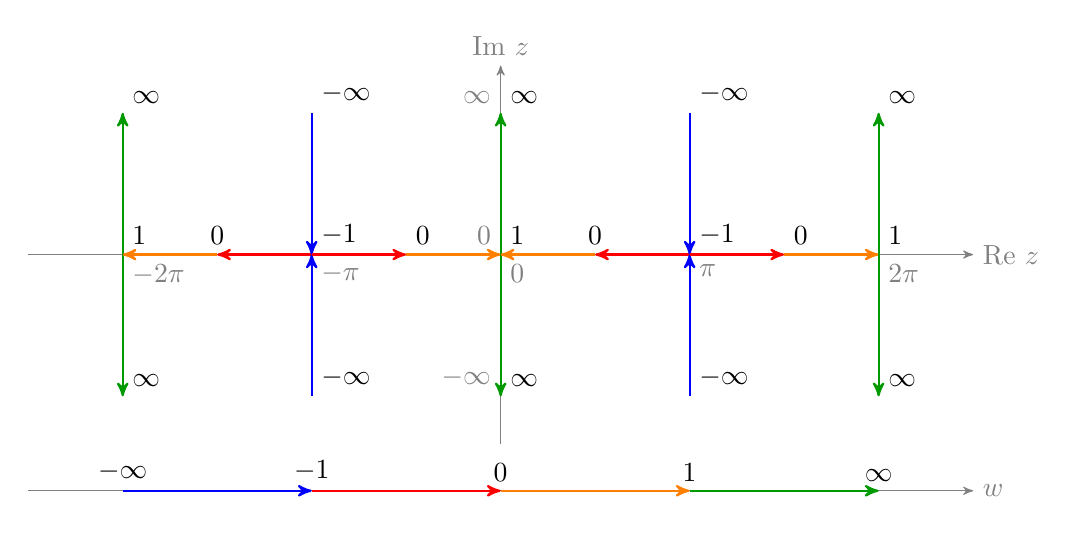
\begin{tikzpicture}[>=stealth', auto, node distance=2cm, scale=1.2]


    \draw[gray, ->] (0,-2) -- (0,2) node[anchor=south]{Im $z$};
    \draw[gray, ->] (-5,0) -- (5,0) node[anchor=west]{Re $z$};

    \begin{scope}
        \draw[thick, ->, orange] (-1, 0) -- (0,0);
        \draw[thick, ->, darkgreen] (0, 0) -- (0,1.5);
        \draw[thick, ->, darkgreen] (0, 0) -- (0,-1.5);
        \draw[thick, ->, orange] (1, 0) -- (0,0);
        \draw[thick, ->, red] (2, 0) -- (1,0);
        \draw[thick, ->, blue] (2,1.5) -- (2, 0);
        \draw[thick, ->, blue] (2,-1.5) -- (2, 0);
        \draw[thick, ->, red] (2, 0) -- (3,0);

        \node[anchor=south west] at (0,1.5) {$\infty$};
        \node[anchor=south west] at (0,-1.5) {$\infty$};
        \node[anchor=south west] at (0,0) {$1$};
        \node[anchor=south] at (1,0) {$0$};
        \node[anchor=south west] at (2,0) {$-1$};
        \node[anchor=south west] at (2,1.5) {$-\infty$};
        \node[anchor=south west] at (2,-1.5) {$-\infty$};
        \node[anchor=south west] at (3,0) {$0$};
    \end{scope}

    \begin{scope}[xshift=4cm]
        \draw[thick, ->, orange] (-1, 0) -- (0,0);
        \draw[thick, ->, darkgreen] (0, 0) -- (0,1.5);
        \draw[thick, ->, darkgreen] (0, 0) -- (0,-1.5);
        % \draw[thick, ->, orange] (1, 0) -- (0,0);
        % \draw[thick, ->, red] (2, 0) -- (1,0);
        % \draw[thick, ->, blue] (2,1.5) -- (2, 0);
        % \draw[thick, ->, blue] (2,-1.5) -- (2, 0);
        % \draw[thick, ->, red] (2, 0) -- (3,0);

        \node[anchor=south west] at (0,1.5) {$\infty$};
        \node[anchor=south west] at (0,-1.5) {$\infty$};
        \node[anchor=south west] at (0,0) {$1$};
        % \node[anchor=south] at (1,0) {$0$};
        % \node[anchor=south west] at (2,0) {$-1$};
        % \node[anchor=south west] at (2,1.5) {$-\infty$};
        % \node[anchor=south west] at (2,-1.5) {$-\infty$};
        % \node[anchor=south west] at (3,0) {$0$};
    \end{scope}

    \begin{scope}[xshift=-4cm]
        % \draw[thick, ->, orange] (-1, 0) -- (0,0);
        \draw[thick, ->, darkgreen] (0, 0) -- (0,1.5);
        \draw[thick, ->, darkgreen] (0, 0) -- (0,-1.5);
        \draw[thick, ->, orange] (1, 0) -- (0,0);
        \draw[thick, ->, red] (2, 0) -- (1,0);
        \draw[thick, ->, blue] (2,1.5) -- (2, 0);
        \draw[thick, ->, blue] (2,-1.5) -- (2, 0);
        \draw[thick, ->, red] (2, 0) -- (3,0);

        \node[anchor=south west] at (0,1.5) {$\infty$};
        \node[anchor=south west] at (0,-1.5) {$\infty$};
        \node[anchor=south west] at (0,0) {$1$};
        \node[anchor=south] at (1,0) {$0$};
        \node[anchor=south west] at (2,0) {$-1$};
        \node[anchor=south west] at (2,1.5) {$-\infty$};
        \node[anchor=south west] at (2,-1.5) {$-\infty$};
        \node[anchor=south west] at (3,0) {$0$};
    \end{scope}

    \node[gray, anchor=north west] at (-4,0) {$-2\pi$};
    \node[gray, anchor=north west] at (-2,0) {$-\pi$};
    \node[gray, anchor=north west] at (0,0) {$0$};
    \node[gray, anchor=north west] at (2,0) {$\pi$};
    \node[gray, anchor=north west] at (4,0) {$2\pi$};


    \node[gray, anchor=south east] at (0,-1.5) {$-\infty$};
    \node[gray, anchor=south east] at (0, 0) {$0$};
    \node[gray, anchor=south east] at (0, 1.5) {$\infty$};



    \begin{scope}[yshift=-2.5cm]

        \draw[gray, ->] (-5,0) -- (5,0) node[anchor=west]{$w$};

        \draw[thick, ->, blue]      (-4, 0) -- (-2, 0);
        \draw[thick, ->, red]       (-2, 0) -- (0, 0);
        \draw[thick, ->, orange]    (0, 0) -- (2, 0);
        \draw[thick, ->, darkgreen] (2, 0) -- (4, 0);

        \node[anchor=south] at (-4,0) {$-\infty$};
        \node[anchor=south] at (-2,0) {$-1$};
        \node[anchor=south] at (0,0) {$0$};
        \node[anchor=south] at (2,0) {$1$};
        \node[anchor=south] at (4,0) {$\infty$};

    \end{scope}

\end{tikzpicture}
					}
				\end{center}

			\end{column}
		\end{columns}



	\end{frame}

	\begin{frame}
		\frametitle{Tschebyscheff-Filter}

		\begin{equation*}
			T_N(w) = \cos \left(z_1 \right), \quad z_1 = N~\cos^{-1}(w)
		\end{equation*}

		\begin{center}
			\scalebox{0.85}{
				\begin{tikzpicture}[>=stealth', auto, node distance=2cm, scale=1.2]

    \tikzstyle{zero} = [draw, circle, inner sep =0, minimum height=0.15cm]

    \tikzset{pole/.style={cross out, draw=black, minimum size=(0.15cm-\pgflinewidth), inner sep=0pt, outer sep=0pt}}

    \begin{scope}[xscale=0.5]

        \draw[gray, ->] (0,-2) -- (0,2) node[anchor=south]{Im $z$};
        \draw[gray, ->] (-10,0) -- (10,0) node[anchor=west]{Re $z$};

        \begin{scope}

            \draw[>->, line width=0.05, thick, blue]   (2, 1.5) -- (2,0.05)  -- node[anchor=south, pos=0.5]{$N=1$} (0.1,0.05) -- (0.1,1.5);
            \draw[>->, line width=0.05, thick, orange] (4, 1.5) -- (4,0)     -- node[anchor=south, pos=0.25]{$N=2$} (0,0) -- (0,1.5);
            \draw[>->, line width=0.05, thick, red]    (6, 1.5) -- (6,-0.05) -- node[anchor=south, pos=0.1666]{$N=3$} (-0.1,-0.05) -- (-0.1,1.5);


            \node[zero] at (-7,0) {};
            \node[zero] at (-5,0) {};
            \node[zero] at (-3,0) {};
            \node[zero] at (-1,0) {};
            \node[zero] at (1,0) {};
            \node[zero] at (3,0) {};
            \node[zero] at (5,0) {};
            \node[zero] at (7,0) {};


        \end{scope}

        \node[gray, anchor=north] at (-8,0) {$-4\pi$};
        \node[gray, anchor=north] at (-6,0) {$-3\pi$};
        \node[gray, anchor=north] at (-4,0) {$-2\pi$};
        \node[gray, anchor=north] at (-2,0) {$-\pi$};
        \node[gray, anchor=north] at (2,0) {$\pi$};
        \node[gray, anchor=north] at (4,0) {$2\pi$};
        \node[gray, anchor=north] at (6,0) {$3\pi$};
        \node[gray, anchor=north] at (8,0) {$4\pi$};


        \node[gray, anchor=east] at (0,-1.5) {$-\infty$};
        \node[gray, anchor=east] at (0, 1.5) {$\infty$};

    \end{scope}

\end{tikzpicture}
			}
		\end{center}

	\end{frame}


	\section{Jacobi elliptische Funktionen}

	\begin{frame}
		\frametitle{Jacobi elliptische Funktionen}

		Elliptisches Integral erster Art

		\begin{equation*}
			F(\phi, k)
			=
			\int_{0}^{\phi}
			\frac{
				d\theta
			}{
				\sqrt{
					1-k^2 \sin^2 \theta
				}
			}
			% =
			% \int_{0}^{\phi}
			% \frac{
			% 	dt
			% }{
			% 	\sqrt{
			% 		(1-t^2)(1-k^2 t^2)
			% 	}
			% }
		\end{equation*}

		\begin{equation*}
			K(k)
			=
			\int_{0}^{\pi / 2}
			\frac{
				d\theta
			}{
				\sqrt{
					1-k^2 \sin^2 \theta
				}
			}
		\end{equation*}



	\end{frame}





	\begin{frame}
		\frametitle{Jacobi elliptische Funktionen}

			\begin{equation*}
				\sn^{-1}(w, k)
				=
				F(\phi, k),
				\quad
				\phi = \sin^{-1}(w)
			\end{equation*}

			\begin{align*}
				\sn^{-1}(w, k)
					& =
				\int_{0}^{\phi}
				\frac{
					d\theta
				}{
					\sqrt{
						1-k^2 \sin^2 \theta
					}
				},
				\quad
				\phi = \sin^{-1}(w)
				\\
					& =
				\int_{0}^{w}
				\frac{
					dt
				}{
					\sqrt{
						(1-t^2)(1-k^2 t^2)
					}
				}
			\end{align*}



		\end{frame}

	\begin{frame}
		\frametitle{Jacobi elliptische Funktionen}
		\begin{columns}
			\begin{column}{0.2\textwidth}

				\begin{equation*}
					z = \sn^{-1}(w, k)
				\end{equation*}

				\vspace{0.5cm}

				Integrand:
				\begin{equation*}
					\frac{
						1
					}{
						\sqrt{
							(1-t^2)(1-k^2 t^2)
						}
					}
				\end{equation*}

			\end{column}
			\begin{column}{0.8\textwidth}
				\begin{center}
					\scalebox{0.75}{
						\begin{tikzpicture}[>=stealth', auto, node distance=2cm, scale=1.2, thick]

    \tikzstyle{zero} = [draw, circle, inner sep =0, minimum height=0.15cm]

    \tikzset{pole/.style={cross out, draw=black, minimum size=(0.15cm-\pgflinewidth), inner sep=0pt, outer sep=0pt}}

    \begin{scope}[xscale=0.9, yscale=1.8]

        \fill[yellow!30] (0,0) rectangle (1, 0.5);

        \draw[gray, ->] (0,-1.5) -- (0,1.5) node[anchor=south]{$\mathrm{Im}~z$};
        \draw[gray, ->] (-5,0) -- (5,0) node[anchor=west]{$\mathrm{Re}~z$};


        \clip(-4.5,-1.25) rectangle (4.5,1.25);


        \begin{scope}[xshift=-1cm]

            \foreach \i in {-2,...,2} {
                \foreach \j in {-2,...,1} {
                    \begin{scope}[xshift=\i*4cm, yshift=\j*1cm]
                        \draw[<-, thick, blue!50] (0, 0) -- (0,0.5);
                        \draw[<-, thick, cyan!50] (1, 0) -- (0,0);
                        \draw[<-, thick, darkgreen!50] (2, 0) -- (1,0);
                        \draw[<-, thick, orange!50] (2,0.5) -- (2, 0);
                        \draw[<-, thick, red!50] (1, 0.5) -- (2,0.5);
                        \draw[<-, thick, purple!50] (0, 0.5) -- (1,0.5);
                        \draw[<-, thick, blue!50] (0,1) -- (0,0.5);
                        \draw[<-, thick, orange!50] (2,0.5) -- (2, 1);
                        \draw[<-, thick, red!50] (3, 0.5) -- (2,0.5);
                        \draw[<-, thick, purple!50] (4, 0.5) -- (3,0.5);
                        \draw[<-, thick, darkgreen!50] (2, 0) -- (3,0);
                        \draw[<-, thick, cyan!50] (3, 0) -- (4,0);
                    \end{scope}
                }
            }

            % \pause
            \draw[ultra thick, <-, darkgreen] (2, 0) -- (1,0);
            % \pause
            \draw[ultra thick, <-, orange] (2,0.5) -- (2, 0);
            % \pause
            \draw[ultra thick, <-, red] (1, 0.5) -- (2,0.5);
            % \pause
            \draw[ultra thick, <-, blue] (0, 0) -- (0,0.5);
            \draw[ultra thick, <-, purple] (0, 0.5) -- (1,0.5);
            \draw[ultra thick, <-, cyan] (1, 0) -- (0,0);
            % \pause


            \foreach \i in {-2,...,2} {
                \foreach \j in {-2,...,1} {
                    \begin{scope}[xshift=\i*4cm, yshift=\j*1cm]
                        \node[zero] at ( 1, 0) {};
                        \node[zero] at ( 3, 0) {};
                        \node[pole] at ( 1,0.5) {};
                        \node[pole] at ( 3,0.5) {};
                    \end{scope}
                }
            }

        \end{scope}


        \draw[gray] ( 1,0) +(0,0.05) -- +(0, -0.05) node[inner sep=0, anchor=north west] {\small $K$};
        \draw[gray]  (0, 0.5) +(0.1, 0) -- +(-0.1, 0) node[inner sep=0, anchor=south east]{\small $jK^\prime$};

    \end{scope}

    \node[zero] at (4,3) (n) {};
    \node[anchor=west] at (n.east) {Nullstelle};
    \node[pole, below=0.25cm of n] (n) {};
    \node[anchor=west] at (n.east) {Polstelle};

    \begin{scope}[yshift=-4cm, xscale=0.75]

        \draw[gray, ->] (-6,0) -- (6,0) node[anchor=west]{$w$};

        \draw[ultra thick, ->, purple] (-5, 0) -- (-3, 0);
        \draw[ultra thick, ->, blue]      (-3, 0) -- (-2, 0);
        \draw[ultra thick, ->, cyan]       (-2, 0) -- (0, 0);
        \draw[ultra thick, ->, darkgreen]    (0, 0) -- (2, 0);
        \draw[ultra thick, ->, orange] (2, 0) -- (3, 0);
        \draw[ultra thick, ->, red] (3, 0) -- (5, 0);

        \node[anchor=south] at (-5,0) {$-\infty$};
        \node[anchor=south] at (-3,0) {$-1/k$};
        \node[anchor=south] at (-2,0) {$-1$};
        \node[anchor=south] at (0,0) {$0$};
        \node[anchor=south] at (2,0) {$1$};
        \node[anchor=south] at (3,0) {$1/k$};
        \node[anchor=south] at (5,0) {$\infty$};

    \end{scope}


\end{tikzpicture}
					}
				\end{center}
			\end{column}
		\end{columns}


	\end{frame}

	\begin{frame}
		\frametitle{Fundamentales Rechteck}

		Nullstelle beim ersten Buchstabe, Polstelle beim zweiten Buchstabe

		\begin{center}
			\scalebox{0.8}{
				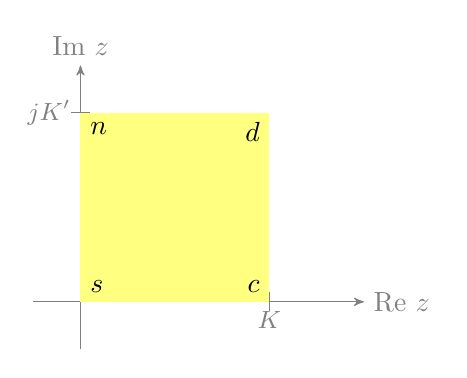
\begin{tikzpicture}[>=stealth', auto, node distance=2cm, scale=1.2]

    \tikzstyle{zero} = [draw, circle, inner sep =0, minimum height=0.15cm]

    \tikzset{pole/.style={cross out, draw=black, minimum size=(0.15cm-\pgflinewidth), inner sep=0pt, outer sep=0pt}}

    \begin{scope}[xscale=2, yscale=2]

        \draw[gray, ->] (0,-0.25) -- (0,1.25) node[anchor=south]{$\mathrm{Im}~z$};
        \draw[gray, ->] (-0.25,0) -- (1.5,0) node[anchor=west]{$\mathrm{Re}~z$};

        \draw[gray] ( 1,0) +(0,0.05) -- +(0, -0.05) node[inner sep=0, anchor=north] {\small $K$};

        \draw[gray]  (0, 1) +(0.05, 0) -- +(-0.05, 0) node[inner sep=0, anchor=east]{\small $jK^\prime$};

        \fill[yellow!50] (0,0) rectangle (1, 1);

        \node[anchor=south east] at ( 1,0) {$c$};
        \node[anchor=north east] at ( 1,1) {$d$};
        \node[anchor=north west] at ( 0,1) {$n$};
        \node[anchor=south west] at ( 0,0) {$s$};

    \end{scope}


\end{tikzpicture}
			}
		\end{center}

	\end{frame}


	\begin{frame}
		\frametitle{Jacobi elliptische Funktionen}

		\begin{equation*}
			z = \cd^{-1}(w, k)
		\end{equation*}

		\begin{center}
			\scalebox{0.7}{
				\begin{tikzpicture}[>=stealth', auto, node distance=2cm, scale=1.2]

    \tikzstyle{zero} = [draw, circle, inner sep =0, minimum height=0.15cm]

    \tikzset{pole/.style={cross out, draw=black, minimum size=(0.15cm-\pgflinewidth), inner sep=0pt, outer sep=0pt}}

    \begin{scope}[xscale=0.9, yscale=1.8]

        \draw[gray, ->] (0,-1.5) -- (0,1.5) node[anchor=south]{$\mathrm{Im}~z$};
        \draw[gray, ->] (-5,0) -- (5,0) node[anchor=west]{$\mathrm{Re}~z$};

        \draw[gray] ( 1,0) +(0,0.1) -- +(0, -0.1) node[inner sep=0, anchor=north] {\small $K$};

        \draw[gray]  (0, 0.5) +(0.1, 0) -- +(-0.1, 0) node[inner sep=0, anchor=east]{\small $jK^\prime$};


        \begin{scope}

            \begin{scope}[xshift=0cm]

                \clip(-4.5,-1.25) rectangle (4.5,1.25);

                \fill[yellow!30] (0,0) rectangle (1, 0.5);


                \draw[ultra thick, ->, darkgreen] (0, 0) -- (0,0.5);
                \draw[ultra thick, ->, orange] (1, 0) -- (0,0);
                \draw[ultra thick, ->, red] (2, 0) -- (1,0);
                \draw[ultra thick, ->, blue] (2,0.5) -- (2, 0);
                \draw[ultra thick, ->, purple] (1, 0.5) -- (2,0.5);
                \draw[ultra thick, ->, cyan] (0, 0.5) -- (1,0.5);



                \foreach \i in {-2,...,1} {
                    \foreach \j in {-2,...,1} {
                        \begin{scope}[xshift=\i*4cm, yshift=\j*1cm]
                            \draw[opacity=0.5, ->, darkgreen] (0, 0) -- (0,0.5);
                            \draw[opacity=0.5, ->, orange] (1, 0) -- (0,0);
                            \draw[opacity=0.5, ->, red] (2, 0) -- (1,0);
                            \draw[opacity=0.5, ->, blue] (2,0.5) -- (2, 0);
                            \draw[opacity=0.5, ->, purple] (1, 0.5) -- (2,0.5);
                            \draw[opacity=0.5, ->, cyan] (0, 0.5) -- (1,0.5);
                            \draw[opacity=0.5, ->, darkgreen] (0,1) -- (0,0.5);
                            \draw[opacity=0.5, ->, blue] (2,0.5) -- (2, 1);
                            \draw[opacity=0.5, ->, purple] (3, 0.5) -- (2,0.5);
                            \draw[opacity=0.5, ->, cyan] (4, 0.5) -- (3,0.5);
                            \draw[opacity=0.5, ->, red] (2, 0) -- (3,0);
                            \draw[opacity=0.5, ->, orange] (3, 0) -- (4,0);

                            \node[zero] at ( 1, 0) {};
                            \node[zero] at ( 3, 0) {};
                            \node[pole] at ( 1,0.5) {};
                            \node[pole] at ( 3,0.5) {};

                        \end{scope}
                    }
                }

            \end{scope}

        \end{scope}

    \end{scope}

    \node[zero] at (4,3) (n) {};
    \node[anchor=west] at (n.east) {Zero};
    \node[pole, below=0.25cm of n] (n) {};
    \node[anchor=west] at (n.east) {Pole};

    \begin{scope}[yshift=-4cm, xscale=0.75]

        \draw[gray, ->] (-6,0) -- (6,0) node[anchor=west]{$w$};

        \draw[thick, ->, purple] (-5, 0) -- (-3, 0);
        \draw[thick, ->, blue]      (-3, 0) -- (-2, 0);
        \draw[thick, ->, red]       (-2, 0) -- (0, 0);
        \draw[thick, ->, orange]    (0, 0) -- (2, 0);
        \draw[thick, ->, darkgreen] (2, 0) -- (3, 0);
        \draw[thick, ->, cyan] (3, 0) -- (5, 0);

        \node[anchor=south] at (-5,0) {$-\infty$};
        \node[anchor=south] at (-3,0) {$-1/k$};
        \node[anchor=south] at (-2,0) {$-1$};
        \node[anchor=south] at (0,0) {$0$};
        \node[anchor=south] at (2,0) {$1$};
        \node[anchor=south] at (3,0) {$1/k$};
        \node[anchor=south] at (5,0) {$\infty$};

    \end{scope}

\end{tikzpicture}

			}
		\end{center}

	\end{frame}

	\section{Elliptisches Filter}

	\begin{frame}
		\frametitle{Elliptisches Filter}

		% \begin{equation*}
		% 	z_1 = N~\frac{K_1}{K}~\cd^{-1}(w, k)
		% \end{equation*}

		\begin{center}
			\scalebox{0.75}{
				\begin{tikzpicture}[>=stealth', auto, node distance=2cm, scale=1.2]

    \tikzstyle{zero} = [draw, circle, inner sep =0, minimum height=0.15cm]
    \tikzstyle{dot} = [fill, circle, inner sep =0, minimum height=0.1cm]

    \tikzset{pole/.style={cross out, draw=black, minimum size=(0.15cm-\pgflinewidth), inner sep=0pt, outer sep=0pt}}

    \begin{scope}[xscale=1.25, yscale=2.5]

        \draw[gray, ->] (0,-0.55) -- (0,1.05) node[anchor=south]{$\mathrm{Im}$};
        \draw[gray, ->] (-1.5,0) -- (6,0) node[anchor=west]{$\mathrm{Re}$};

        % \draw[gray] ( 1,0) +(0,0.05) -- +(0, -0.05) node[inner sep=0, anchor=north] {\small $K_1$};
        % \draw[gray] ( 5,0) +(0,0.05) -- +(0, -0.05) node[inner sep=0, anchor=north] {\small $5K_1$};
        % \draw[gray]  (0, 0.5) +(0.1, 0) -- +(-0.1, 0) node[inner sep=0, anchor=east]{\small $jK^\prime_1$};

        \begin{scope}

            \clip(-1.5,-0.75) rectangle (6.8,1.25);

            % \draw[>->, line width=0.05, thick, blue]   (1, 0.45) -- (2, 0.45) -- (2, 0.05) -- ( 0.1, 0.05) -- ( 0.1,0.45) -- (1, 0.45);
            % \draw[>->, line width=0.05, thick, orange] (2, 0.5 ) -- (4, 0.5 ) -- (4, 0   ) -- ( 0  , 0   ) -- ( 0  ,0.5 ) -- (2, 0.5 );
            % \draw[>->, line width=0.05, thick, red]    (3, 0.55) -- (6, 0.55) -- (6,-0.05) -- (-0.1,-0.05) -- (-0.1,0.55) -- (3, 0.55);
            % \node[blue] at (1, 0.25) {$N=1$};
            % \node[orange] at (3, 0.25) {$N=2$};
            % \node[red] at (5, 0.25) {$N=3$};



            % \draw[line width=0.1cm, fill, red!50] (0,0) rectangle (3, 0.5);
            % \draw[line width=0.05cm, fill, orange!50] (0,0) rectangle (2, 0.5);
            % \fill[yellow!50] (0,0) rectangle (1, 0.5);
            % \node[] at (0.5, 0.25) {\small $N=1$};
            % \node[] at (1.5, 0.25) {\small $N=2$};
            % \node[] at (2.5, 0.25) {\small $N=3$};

            % \fill[orange!30] (0,0) rectangle (5, 0.5);
            \fill[yellow!30] (0,0) rectangle (1, 0.5);
            \node[] at (2.5, 0.25) {\small $N=5$};


            % \draw[decorate,decoration={brace,amplitude=3pt,mirror}, yshift=0.05cm]
            %     (5,0.5) node(t_k_unten){} -- node[above, yshift=0.1cm]{$NK_1$}
            %     (0,0.5) node(t_k_opt_unten){};

            % \draw[decorate,decoration={brace,amplitude=3pt,mirror}, xshift=0.1cm]
            %     (5,0) node(t_k_unten){} -- node[right, xshift=0.1cm]{$K^\prime \frac{K_1N}{K} = K^\prime_1$}
            %     (5,0.5) node(t_k_opt_unten){};

            \foreach \i in {-2,...,1} {
                \foreach \j in {-2,...,1} {
                    \begin{scope}[xshift=\i*4cm, yshift=\j*1cm]

                        \node[zero] at ( 1, 0) {};
                        \node[zero] at ( 3, 0) {};
                        \node[pole] at ( 1,0.5) {};
                        \node[pole] at ( 3,0.5) {};

                    \end{scope}
                }
            }




            \draw[ultra thick, ->, darkgreen] (5, 0) -- node[yshift=-0.4cm]{Durchlassbereich} (0,0);
            \draw[ultra thick, ->, orange] (-0, 0) --  node[align=center]{Übergangs-\\berech} (0,0.5);
            \draw[ultra thick, ->, red] (0,0.5) -- node[align=center, yshift=0.4cm]{Sperrbereich} (5, 0.5);

            \draw (4,0  )  node[dot]{} node[anchor=south]      {\small $1$};
            \draw (2,0  )  node[dot]{} node[anchor=south]      {\small $-1$};
            \draw (0,0  )  node[dot]{} node[anchor=south west] {\small $1$};
            \draw (0,0.5)  node[dot]{} node[anchor=north west] {\small $1/k$};
            \draw (2,0.5)  node[dot]{} node[anchor=north]      {\small $-1/k$};
            \draw (4,0.5)  node[dot]{} node[anchor=north]      {\small $1/k$};



        \end{scope}


    \end{scope}

\end{tikzpicture}
			}
		\end{center}

	\end{frame}

	\begin{frame}
		\frametitle{Periodizität in realer und imaginärer Richtung}

		\begin{center}
			%% Creator: Matplotlib, PGF backend
%%
%% To include the figure in your LaTeX document, write
%%   \input{<filename>.pgf}
%%
%% Make sure the required packages are loaded in your preamble
%%   \usepackage{pgf}
%%
%% Also ensure that all the required font packages are loaded; for instance,
%% the lmodern package is sometimes necessary when using math font.
%%   \usepackage{lmodern}
%%
%% Figures using additional raster images can only be included by \input if
%% they are in the same directory as the main LaTeX file. For loading figures
%% from other directories you can use the `import` package
%%   \usepackage{import}
%%
%% and then include the figures with
%%   \import{<path to file>}{<filename>.pgf}
%%
%% Matplotlib used the following preamble
%%
\begingroup%
\makeatletter%
\begin{pgfpicture}%
\pgfpathrectangle{\pgfpointorigin}{\pgfqpoint{5.000000in}{2.500000in}}%
\pgfusepath{use as bounding box, clip}%
\begin{pgfscope}%
\pgfsetbuttcap%
\pgfsetmiterjoin%
\pgfsetlinewidth{0.000000pt}%
\definecolor{currentstroke}{rgb}{1.000000,1.000000,1.000000}%
\pgfsetstrokecolor{currentstroke}%
\pgfsetstrokeopacity{0.000000}%
\pgfsetdash{}{0pt}%
\pgfpathmoveto{\pgfqpoint{0.000000in}{0.000000in}}%
\pgfpathlineto{\pgfqpoint{5.000000in}{0.000000in}}%
\pgfpathlineto{\pgfqpoint{5.000000in}{2.500000in}}%
\pgfpathlineto{\pgfqpoint{0.000000in}{2.500000in}}%
\pgfpathlineto{\pgfqpoint{0.000000in}{0.000000in}}%
\pgfpathclose%
\pgfusepath{}%
\end{pgfscope}%
\begin{pgfscope}%
\pgfsetbuttcap%
\pgfsetmiterjoin%
\definecolor{currentfill}{rgb}{1.000000,1.000000,1.000000}%
\pgfsetfillcolor{currentfill}%
\pgfsetlinewidth{0.000000pt}%
\definecolor{currentstroke}{rgb}{0.000000,0.000000,0.000000}%
\pgfsetstrokecolor{currentstroke}%
\pgfsetstrokeopacity{0.000000}%
\pgfsetdash{}{0pt}%
\pgfpathmoveto{\pgfqpoint{0.316407in}{0.548769in}}%
\pgfpathlineto{\pgfqpoint{2.256930in}{0.548769in}}%
\pgfpathlineto{\pgfqpoint{2.256930in}{2.301955in}}%
\pgfpathlineto{\pgfqpoint{0.316407in}{2.301955in}}%
\pgfpathlineto{\pgfqpoint{0.316407in}{0.548769in}}%
\pgfpathclose%
\pgfusepath{fill}%
\end{pgfscope}%
\begin{pgfscope}%
\pgfsetbuttcap%
\pgfsetroundjoin%
\definecolor{currentfill}{rgb}{0.000000,0.000000,0.000000}%
\pgfsetfillcolor{currentfill}%
\pgfsetlinewidth{0.803000pt}%
\definecolor{currentstroke}{rgb}{0.000000,0.000000,0.000000}%
\pgfsetstrokecolor{currentstroke}%
\pgfsetdash{}{0pt}%
\pgfsys@defobject{currentmarker}{\pgfqpoint{0.000000in}{-0.048611in}}{\pgfqpoint{0.000000in}{0.000000in}}{%
\pgfpathmoveto{\pgfqpoint{0.000000in}{0.000000in}}%
\pgfpathlineto{\pgfqpoint{0.000000in}{-0.048611in}}%
\pgfusepath{stroke,fill}%
}%
\begin{pgfscope}%
\pgfsys@transformshift{0.316407in}{0.548769in}%
\pgfsys@useobject{currentmarker}{}%
\end{pgfscope}%
\end{pgfscope}%
\begin{pgfscope}%
\definecolor{textcolor}{rgb}{0.000000,0.000000,0.000000}%
\pgfsetstrokecolor{textcolor}%
\pgfsetfillcolor{textcolor}%
\pgftext[x=0.316407in,y=0.451547in,,top]{\color{textcolor}\rmfamily\fontsize{10.000000}{12.000000}\selectfont \(\displaystyle {0.00}\)}%
\end{pgfscope}%
\begin{pgfscope}%
\pgfsetbuttcap%
\pgfsetroundjoin%
\definecolor{currentfill}{rgb}{0.000000,0.000000,0.000000}%
\pgfsetfillcolor{currentfill}%
\pgfsetlinewidth{0.803000pt}%
\definecolor{currentstroke}{rgb}{0.000000,0.000000,0.000000}%
\pgfsetstrokecolor{currentstroke}%
\pgfsetdash{}{0pt}%
\pgfsys@defobject{currentmarker}{\pgfqpoint{0.000000in}{-0.048611in}}{\pgfqpoint{0.000000in}{0.000000in}}{%
\pgfpathmoveto{\pgfqpoint{0.000000in}{0.000000in}}%
\pgfpathlineto{\pgfqpoint{0.000000in}{-0.048611in}}%
\pgfusepath{stroke,fill}%
}%
\begin{pgfscope}%
\pgfsys@transformshift{0.801538in}{0.548769in}%
\pgfsys@useobject{currentmarker}{}%
\end{pgfscope}%
\end{pgfscope}%
\begin{pgfscope}%
\definecolor{textcolor}{rgb}{0.000000,0.000000,0.000000}%
\pgfsetstrokecolor{textcolor}%
\pgfsetfillcolor{textcolor}%
\pgftext[x=0.801538in,y=0.451547in,,top]{\color{textcolor}\rmfamily\fontsize{10.000000}{12.000000}\selectfont \(\displaystyle {0.25}\)}%
\end{pgfscope}%
\begin{pgfscope}%
\pgfsetbuttcap%
\pgfsetroundjoin%
\definecolor{currentfill}{rgb}{0.000000,0.000000,0.000000}%
\pgfsetfillcolor{currentfill}%
\pgfsetlinewidth{0.803000pt}%
\definecolor{currentstroke}{rgb}{0.000000,0.000000,0.000000}%
\pgfsetstrokecolor{currentstroke}%
\pgfsetdash{}{0pt}%
\pgfsys@defobject{currentmarker}{\pgfqpoint{0.000000in}{-0.048611in}}{\pgfqpoint{0.000000in}{0.000000in}}{%
\pgfpathmoveto{\pgfqpoint{0.000000in}{0.000000in}}%
\pgfpathlineto{\pgfqpoint{0.000000in}{-0.048611in}}%
\pgfusepath{stroke,fill}%
}%
\begin{pgfscope}%
\pgfsys@transformshift{1.286669in}{0.548769in}%
\pgfsys@useobject{currentmarker}{}%
\end{pgfscope}%
\end{pgfscope}%
\begin{pgfscope}%
\definecolor{textcolor}{rgb}{0.000000,0.000000,0.000000}%
\pgfsetstrokecolor{textcolor}%
\pgfsetfillcolor{textcolor}%
\pgftext[x=1.286669in,y=0.451547in,,top]{\color{textcolor}\rmfamily\fontsize{10.000000}{12.000000}\selectfont \(\displaystyle {0.50}\)}%
\end{pgfscope}%
\begin{pgfscope}%
\pgfsetbuttcap%
\pgfsetroundjoin%
\definecolor{currentfill}{rgb}{0.000000,0.000000,0.000000}%
\pgfsetfillcolor{currentfill}%
\pgfsetlinewidth{0.803000pt}%
\definecolor{currentstroke}{rgb}{0.000000,0.000000,0.000000}%
\pgfsetstrokecolor{currentstroke}%
\pgfsetdash{}{0pt}%
\pgfsys@defobject{currentmarker}{\pgfqpoint{0.000000in}{-0.048611in}}{\pgfqpoint{0.000000in}{0.000000in}}{%
\pgfpathmoveto{\pgfqpoint{0.000000in}{0.000000in}}%
\pgfpathlineto{\pgfqpoint{0.000000in}{-0.048611in}}%
\pgfusepath{stroke,fill}%
}%
\begin{pgfscope}%
\pgfsys@transformshift{1.771800in}{0.548769in}%
\pgfsys@useobject{currentmarker}{}%
\end{pgfscope}%
\end{pgfscope}%
\begin{pgfscope}%
\definecolor{textcolor}{rgb}{0.000000,0.000000,0.000000}%
\pgfsetstrokecolor{textcolor}%
\pgfsetfillcolor{textcolor}%
\pgftext[x=1.771800in,y=0.451547in,,top]{\color{textcolor}\rmfamily\fontsize{10.000000}{12.000000}\selectfont \(\displaystyle {0.75}\)}%
\end{pgfscope}%
\begin{pgfscope}%
\pgfsetbuttcap%
\pgfsetroundjoin%
\definecolor{currentfill}{rgb}{0.000000,0.000000,0.000000}%
\pgfsetfillcolor{currentfill}%
\pgfsetlinewidth{0.803000pt}%
\definecolor{currentstroke}{rgb}{0.000000,0.000000,0.000000}%
\pgfsetstrokecolor{currentstroke}%
\pgfsetdash{}{0pt}%
\pgfsys@defobject{currentmarker}{\pgfqpoint{0.000000in}{-0.048611in}}{\pgfqpoint{0.000000in}{0.000000in}}{%
\pgfpathmoveto{\pgfqpoint{0.000000in}{0.000000in}}%
\pgfpathlineto{\pgfqpoint{0.000000in}{-0.048611in}}%
\pgfusepath{stroke,fill}%
}%
\begin{pgfscope}%
\pgfsys@transformshift{2.256930in}{0.548769in}%
\pgfsys@useobject{currentmarker}{}%
\end{pgfscope}%
\end{pgfscope}%
\begin{pgfscope}%
\definecolor{textcolor}{rgb}{0.000000,0.000000,0.000000}%
\pgfsetstrokecolor{textcolor}%
\pgfsetfillcolor{textcolor}%
\pgftext[x=2.256930in,y=0.451547in,,top]{\color{textcolor}\rmfamily\fontsize{10.000000}{12.000000}\selectfont \(\displaystyle {1.00}\)}%
\end{pgfscope}%
\begin{pgfscope}%
\definecolor{textcolor}{rgb}{0.000000,0.000000,0.000000}%
\pgfsetstrokecolor{textcolor}%
\pgfsetfillcolor{textcolor}%
\pgftext[x=1.286669in,y=0.272534in,,top]{\color{textcolor}\rmfamily\fontsize{10.000000}{12.000000}\selectfont \(\displaystyle k\)}%
\end{pgfscope}%
\begin{pgfscope}%
\pgfsetbuttcap%
\pgfsetroundjoin%
\definecolor{currentfill}{rgb}{0.000000,0.000000,0.000000}%
\pgfsetfillcolor{currentfill}%
\pgfsetlinewidth{0.803000pt}%
\definecolor{currentstroke}{rgb}{0.000000,0.000000,0.000000}%
\pgfsetstrokecolor{currentstroke}%
\pgfsetdash{}{0pt}%
\pgfsys@defobject{currentmarker}{\pgfqpoint{-0.048611in}{0.000000in}}{\pgfqpoint{-0.000000in}{0.000000in}}{%
\pgfpathmoveto{\pgfqpoint{-0.000000in}{0.000000in}}%
\pgfpathlineto{\pgfqpoint{-0.048611in}{0.000000in}}%
\pgfusepath{stroke,fill}%
}%
\begin{pgfscope}%
\pgfsys@transformshift{0.316407in}{0.548769in}%
\pgfsys@useobject{currentmarker}{}%
\end{pgfscope}%
\end{pgfscope}%
\begin{pgfscope}%
\definecolor{textcolor}{rgb}{0.000000,0.000000,0.000000}%
\pgfsetstrokecolor{textcolor}%
\pgfsetfillcolor{textcolor}%
\pgftext[x=0.149740in, y=0.500544in, left, base]{\color{textcolor}\rmfamily\fontsize{10.000000}{12.000000}\selectfont \(\displaystyle {0}\)}%
\end{pgfscope}%
\begin{pgfscope}%
\pgfsetbuttcap%
\pgfsetroundjoin%
\definecolor{currentfill}{rgb}{0.000000,0.000000,0.000000}%
\pgfsetfillcolor{currentfill}%
\pgfsetlinewidth{0.803000pt}%
\definecolor{currentstroke}{rgb}{0.000000,0.000000,0.000000}%
\pgfsetstrokecolor{currentstroke}%
\pgfsetdash{}{0pt}%
\pgfsys@defobject{currentmarker}{\pgfqpoint{-0.048611in}{0.000000in}}{\pgfqpoint{-0.000000in}{0.000000in}}{%
\pgfpathmoveto{\pgfqpoint{-0.000000in}{0.000000in}}%
\pgfpathlineto{\pgfqpoint{-0.048611in}{0.000000in}}%
\pgfusepath{stroke,fill}%
}%
\begin{pgfscope}%
\pgfsys@transformshift{0.316407in}{0.987065in}%
\pgfsys@useobject{currentmarker}{}%
\end{pgfscope}%
\end{pgfscope}%
\begin{pgfscope}%
\definecolor{textcolor}{rgb}{0.000000,0.000000,0.000000}%
\pgfsetstrokecolor{textcolor}%
\pgfsetfillcolor{textcolor}%
\pgftext[x=0.149740in, y=0.938840in, left, base]{\color{textcolor}\rmfamily\fontsize{10.000000}{12.000000}\selectfont \(\displaystyle {1}\)}%
\end{pgfscope}%
\begin{pgfscope}%
\pgfsetbuttcap%
\pgfsetroundjoin%
\definecolor{currentfill}{rgb}{0.000000,0.000000,0.000000}%
\pgfsetfillcolor{currentfill}%
\pgfsetlinewidth{0.803000pt}%
\definecolor{currentstroke}{rgb}{0.000000,0.000000,0.000000}%
\pgfsetstrokecolor{currentstroke}%
\pgfsetdash{}{0pt}%
\pgfsys@defobject{currentmarker}{\pgfqpoint{-0.048611in}{0.000000in}}{\pgfqpoint{-0.000000in}{0.000000in}}{%
\pgfpathmoveto{\pgfqpoint{-0.000000in}{0.000000in}}%
\pgfpathlineto{\pgfqpoint{-0.048611in}{0.000000in}}%
\pgfusepath{stroke,fill}%
}%
\begin{pgfscope}%
\pgfsys@transformshift{0.316407in}{1.425362in}%
\pgfsys@useobject{currentmarker}{}%
\end{pgfscope}%
\end{pgfscope}%
\begin{pgfscope}%
\definecolor{textcolor}{rgb}{0.000000,0.000000,0.000000}%
\pgfsetstrokecolor{textcolor}%
\pgfsetfillcolor{textcolor}%
\pgftext[x=0.149740in, y=1.377137in, left, base]{\color{textcolor}\rmfamily\fontsize{10.000000}{12.000000}\selectfont \(\displaystyle {2}\)}%
\end{pgfscope}%
\begin{pgfscope}%
\pgfsetbuttcap%
\pgfsetroundjoin%
\definecolor{currentfill}{rgb}{0.000000,0.000000,0.000000}%
\pgfsetfillcolor{currentfill}%
\pgfsetlinewidth{0.803000pt}%
\definecolor{currentstroke}{rgb}{0.000000,0.000000,0.000000}%
\pgfsetstrokecolor{currentstroke}%
\pgfsetdash{}{0pt}%
\pgfsys@defobject{currentmarker}{\pgfqpoint{-0.048611in}{0.000000in}}{\pgfqpoint{-0.000000in}{0.000000in}}{%
\pgfpathmoveto{\pgfqpoint{-0.000000in}{0.000000in}}%
\pgfpathlineto{\pgfqpoint{-0.048611in}{0.000000in}}%
\pgfusepath{stroke,fill}%
}%
\begin{pgfscope}%
\pgfsys@transformshift{0.316407in}{1.863658in}%
\pgfsys@useobject{currentmarker}{}%
\end{pgfscope}%
\end{pgfscope}%
\begin{pgfscope}%
\definecolor{textcolor}{rgb}{0.000000,0.000000,0.000000}%
\pgfsetstrokecolor{textcolor}%
\pgfsetfillcolor{textcolor}%
\pgftext[x=0.149740in, y=1.815433in, left, base]{\color{textcolor}\rmfamily\fontsize{10.000000}{12.000000}\selectfont \(\displaystyle {3}\)}%
\end{pgfscope}%
\begin{pgfscope}%
\pgfsetbuttcap%
\pgfsetroundjoin%
\definecolor{currentfill}{rgb}{0.000000,0.000000,0.000000}%
\pgfsetfillcolor{currentfill}%
\pgfsetlinewidth{0.803000pt}%
\definecolor{currentstroke}{rgb}{0.000000,0.000000,0.000000}%
\pgfsetstrokecolor{currentstroke}%
\pgfsetdash{}{0pt}%
\pgfsys@defobject{currentmarker}{\pgfqpoint{-0.048611in}{0.000000in}}{\pgfqpoint{-0.000000in}{0.000000in}}{%
\pgfpathmoveto{\pgfqpoint{-0.000000in}{0.000000in}}%
\pgfpathlineto{\pgfqpoint{-0.048611in}{0.000000in}}%
\pgfusepath{stroke,fill}%
}%
\begin{pgfscope}%
\pgfsys@transformshift{0.316407in}{2.301955in}%
\pgfsys@useobject{currentmarker}{}%
\end{pgfscope}%
\end{pgfscope}%
\begin{pgfscope}%
\definecolor{textcolor}{rgb}{0.000000,0.000000,0.000000}%
\pgfsetstrokecolor{textcolor}%
\pgfsetfillcolor{textcolor}%
\pgftext[x=0.149740in, y=2.253730in, left, base]{\color{textcolor}\rmfamily\fontsize{10.000000}{12.000000}\selectfont \(\displaystyle {4}\)}%
\end{pgfscope}%
\begin{pgfscope}%
\pgfpathrectangle{\pgfqpoint{0.316407in}{0.548769in}}{\pgfqpoint{1.940523in}{1.753186in}}%
\pgfusepath{clip}%
\pgfsetrectcap%
\pgfsetroundjoin%
\pgfsetlinewidth{1.003750pt}%
\definecolor{currentstroke}{rgb}{0.121569,0.466667,0.705882}%
\pgfsetstrokecolor{currentstroke}%
\pgfsetdash{}{0pt}%
\pgfpathmoveto{\pgfqpoint{0.316427in}{1.237243in}}%
\pgfpathlineto{\pgfqpoint{0.316601in}{1.237243in}}%
\pgfpathlineto{\pgfqpoint{0.318348in}{1.237244in}}%
\pgfpathlineto{\pgfqpoint{0.335813in}{1.237261in}}%
\pgfpathlineto{\pgfqpoint{0.355218in}{1.237312in}}%
\pgfpathlineto{\pgfqpoint{0.374623in}{1.237398in}}%
\pgfpathlineto{\pgfqpoint{0.394028in}{1.237519in}}%
\pgfpathlineto{\pgfqpoint{0.413434in}{1.237674in}}%
\pgfpathlineto{\pgfqpoint{0.432839in}{1.237864in}}%
\pgfpathlineto{\pgfqpoint{0.452244in}{1.238089in}}%
\pgfpathlineto{\pgfqpoint{0.471649in}{1.238349in}}%
\pgfpathlineto{\pgfqpoint{0.491054in}{1.238644in}}%
\pgfpathlineto{\pgfqpoint{0.510460in}{1.238974in}}%
\pgfpathlineto{\pgfqpoint{0.529865in}{1.239340in}}%
\pgfpathlineto{\pgfqpoint{0.549270in}{1.239742in}}%
\pgfpathlineto{\pgfqpoint{0.568675in}{1.240180in}}%
\pgfpathlineto{\pgfqpoint{0.588081in}{1.240655in}}%
\pgfpathlineto{\pgfqpoint{0.607486in}{1.241166in}}%
\pgfpathlineto{\pgfqpoint{0.626891in}{1.241714in}}%
\pgfpathlineto{\pgfqpoint{0.646296in}{1.242300in}}%
\pgfpathlineto{\pgfqpoint{0.665702in}{1.242924in}}%
\pgfpathlineto{\pgfqpoint{0.685107in}{1.243586in}}%
\pgfpathlineto{\pgfqpoint{0.704512in}{1.244287in}}%
\pgfpathlineto{\pgfqpoint{0.723917in}{1.245028in}}%
\pgfpathlineto{\pgfqpoint{0.743322in}{1.245809in}}%
\pgfpathlineto{\pgfqpoint{0.762728in}{1.246630in}}%
\pgfpathlineto{\pgfqpoint{0.782133in}{1.247492in}}%
\pgfpathlineto{\pgfqpoint{0.801538in}{1.248396in}}%
\pgfpathlineto{\pgfqpoint{0.820943in}{1.249343in}}%
\pgfpathlineto{\pgfqpoint{0.840349in}{1.250333in}}%
\pgfpathlineto{\pgfqpoint{0.859754in}{1.251367in}}%
\pgfpathlineto{\pgfqpoint{0.879159in}{1.252446in}}%
\pgfpathlineto{\pgfqpoint{0.898564in}{1.253571in}}%
\pgfpathlineto{\pgfqpoint{0.917969in}{1.254743in}}%
\pgfpathlineto{\pgfqpoint{0.937375in}{1.255962in}}%
\pgfpathlineto{\pgfqpoint{0.956780in}{1.257230in}}%
\pgfpathlineto{\pgfqpoint{0.976185in}{1.258548in}}%
\pgfpathlineto{\pgfqpoint{0.995590in}{1.259917in}}%
\pgfpathlineto{\pgfqpoint{1.014996in}{1.261339in}}%
\pgfpathlineto{\pgfqpoint{1.034401in}{1.262814in}}%
\pgfpathlineto{\pgfqpoint{1.053806in}{1.264344in}}%
\pgfpathlineto{\pgfqpoint{1.073211in}{1.265930in}}%
\pgfpathlineto{\pgfqpoint{1.092617in}{1.267575in}}%
\pgfpathlineto{\pgfqpoint{1.112022in}{1.269279in}}%
\pgfpathlineto{\pgfqpoint{1.131427in}{1.271045in}}%
\pgfpathlineto{\pgfqpoint{1.150832in}{1.272874in}}%
\pgfpathlineto{\pgfqpoint{1.170237in}{1.274768in}}%
\pgfpathlineto{\pgfqpoint{1.189643in}{1.276729in}}%
\pgfpathlineto{\pgfqpoint{1.209048in}{1.278760in}}%
\pgfpathlineto{\pgfqpoint{1.228453in}{1.280863in}}%
\pgfpathlineto{\pgfqpoint{1.247858in}{1.283040in}}%
\pgfpathlineto{\pgfqpoint{1.267264in}{1.285294in}}%
\pgfpathlineto{\pgfqpoint{1.286669in}{1.287627in}}%
\pgfpathlineto{\pgfqpoint{1.306074in}{1.290044in}}%
\pgfpathlineto{\pgfqpoint{1.325479in}{1.292546in}}%
\pgfpathlineto{\pgfqpoint{1.344884in}{1.295137in}}%
\pgfpathlineto{\pgfqpoint{1.364290in}{1.297822in}}%
\pgfpathlineto{\pgfqpoint{1.383695in}{1.300603in}}%
\pgfpathlineto{\pgfqpoint{1.403100in}{1.303485in}}%
\pgfpathlineto{\pgfqpoint{1.422505in}{1.306473in}}%
\pgfpathlineto{\pgfqpoint{1.441911in}{1.309570in}}%
\pgfpathlineto{\pgfqpoint{1.461316in}{1.312784in}}%
\pgfpathlineto{\pgfqpoint{1.480721in}{1.316118in}}%
\pgfpathlineto{\pgfqpoint{1.500126in}{1.319579in}}%
\pgfpathlineto{\pgfqpoint{1.519532in}{1.323174in}}%
\pgfpathlineto{\pgfqpoint{1.538937in}{1.326910in}}%
\pgfpathlineto{\pgfqpoint{1.558342in}{1.330793in}}%
\pgfpathlineto{\pgfqpoint{1.577747in}{1.334833in}}%
\pgfpathlineto{\pgfqpoint{1.597152in}{1.339039in}}%
\pgfpathlineto{\pgfqpoint{1.616558in}{1.343420in}}%
\pgfpathlineto{\pgfqpoint{1.635963in}{1.347988in}}%
\pgfpathlineto{\pgfqpoint{1.655368in}{1.352753in}}%
\pgfpathlineto{\pgfqpoint{1.674773in}{1.357730in}}%
\pgfpathlineto{\pgfqpoint{1.694179in}{1.362933in}}%
\pgfpathlineto{\pgfqpoint{1.713584in}{1.368377in}}%
\pgfpathlineto{\pgfqpoint{1.732989in}{1.374081in}}%
\pgfpathlineto{\pgfqpoint{1.752394in}{1.380064in}}%
\pgfpathlineto{\pgfqpoint{1.771800in}{1.386349in}}%
\pgfpathlineto{\pgfqpoint{1.791205in}{1.392961in}}%
\pgfpathlineto{\pgfqpoint{1.810610in}{1.399927in}}%
\pgfpathlineto{\pgfqpoint{1.830015in}{1.407281in}}%
\pgfpathlineto{\pgfqpoint{1.849420in}{1.415059in}}%
\pgfpathlineto{\pgfqpoint{1.868826in}{1.423303in}}%
\pgfpathlineto{\pgfqpoint{1.888231in}{1.432062in}}%
\pgfpathlineto{\pgfqpoint{1.907636in}{1.441392in}}%
\pgfpathlineto{\pgfqpoint{1.927041in}{1.451361in}}%
\pgfpathlineto{\pgfqpoint{1.946447in}{1.462048in}}%
\pgfpathlineto{\pgfqpoint{1.965852in}{1.473546in}}%
\pgfpathlineto{\pgfqpoint{1.985257in}{1.485971in}}%
\pgfpathlineto{\pgfqpoint{2.004662in}{1.499462in}}%
\pgfpathlineto{\pgfqpoint{2.024067in}{1.514194in}}%
\pgfpathlineto{\pgfqpoint{2.043473in}{1.530388in}}%
\pgfpathlineto{\pgfqpoint{2.062878in}{1.548326in}}%
\pgfpathlineto{\pgfqpoint{2.082283in}{1.568383in}}%
\pgfpathlineto{\pgfqpoint{2.101688in}{1.591069in}}%
\pgfpathlineto{\pgfqpoint{2.121094in}{1.617098in}}%
\pgfpathlineto{\pgfqpoint{2.140499in}{1.647519in}}%
\pgfpathlineto{\pgfqpoint{2.159904in}{1.683962in}}%
\pgfpathlineto{\pgfqpoint{2.179309in}{1.729164in}}%
\pgfpathlineto{\pgfqpoint{2.198715in}{1.788269in}}%
\pgfpathlineto{\pgfqpoint{2.218120in}{1.872854in}}%
\pgfpathlineto{\pgfqpoint{2.237525in}{2.019955in}}%
\pgfpathlineto{\pgfqpoint{2.247876in}{2.315844in}}%
\pgfusepath{stroke}%
\end{pgfscope}%
\begin{pgfscope}%
\pgfpathrectangle{\pgfqpoint{0.316407in}{0.548769in}}{\pgfqpoint{1.940523in}{1.753186in}}%
\pgfusepath{clip}%
\pgfsetrectcap%
\pgfsetroundjoin%
\pgfsetlinewidth{1.003750pt}%
\definecolor{currentstroke}{rgb}{1.000000,0.498039,0.054902}%
\pgfsetstrokecolor{currentstroke}%
\pgfsetdash{}{0pt}%
\pgfpathmoveto{\pgfqpoint{0.454821in}{2.315844in}}%
\pgfpathlineto{\pgfqpoint{0.471649in}{2.265444in}}%
\pgfpathlineto{\pgfqpoint{0.491054in}{2.214262in}}%
\pgfpathlineto{\pgfqpoint{0.510460in}{2.168554in}}%
\pgfpathlineto{\pgfqpoint{0.529865in}{2.127278in}}%
\pgfpathlineto{\pgfqpoint{0.549270in}{2.089666in}}%
\pgfpathlineto{\pgfqpoint{0.568675in}{2.055132in}}%
\pgfpathlineto{\pgfqpoint{0.588081in}{2.023222in}}%
\pgfpathlineto{\pgfqpoint{0.607486in}{1.993575in}}%
\pgfpathlineto{\pgfqpoint{0.626891in}{1.965899in}}%
\pgfpathlineto{\pgfqpoint{0.646296in}{1.939958in}}%
\pgfpathlineto{\pgfqpoint{0.665702in}{1.915554in}}%
\pgfpathlineto{\pgfqpoint{0.685107in}{1.892522in}}%
\pgfpathlineto{\pgfqpoint{0.704512in}{1.870720in}}%
\pgfpathlineto{\pgfqpoint{0.723917in}{1.850031in}}%
\pgfpathlineto{\pgfqpoint{0.743322in}{1.830351in}}%
\pgfpathlineto{\pgfqpoint{0.762728in}{1.811591in}}%
\pgfpathlineto{\pgfqpoint{0.782133in}{1.793672in}}%
\pgfpathlineto{\pgfqpoint{0.801538in}{1.776528in}}%
\pgfpathlineto{\pgfqpoint{0.820943in}{1.760096in}}%
\pgfpathlineto{\pgfqpoint{0.840349in}{1.744324in}}%
\pgfpathlineto{\pgfqpoint{0.859754in}{1.729164in}}%
\pgfpathlineto{\pgfqpoint{0.879159in}{1.714573in}}%
\pgfpathlineto{\pgfqpoint{0.898564in}{1.700513in}}%
\pgfpathlineto{\pgfqpoint{0.917969in}{1.686948in}}%
\pgfpathlineto{\pgfqpoint{0.937375in}{1.673849in}}%
\pgfpathlineto{\pgfqpoint{0.956780in}{1.661185in}}%
\pgfpathlineto{\pgfqpoint{0.976185in}{1.648932in}}%
\pgfpathlineto{\pgfqpoint{0.995590in}{1.637065in}}%
\pgfpathlineto{\pgfqpoint{1.014996in}{1.625563in}}%
\pgfpathlineto{\pgfqpoint{1.034401in}{1.614406in}}%
\pgfpathlineto{\pgfqpoint{1.053806in}{1.603575in}}%
\pgfpathlineto{\pgfqpoint{1.073211in}{1.593053in}}%
\pgfpathlineto{\pgfqpoint{1.092617in}{1.582826in}}%
\pgfpathlineto{\pgfqpoint{1.112022in}{1.572877in}}%
\pgfpathlineto{\pgfqpoint{1.131427in}{1.563195in}}%
\pgfpathlineto{\pgfqpoint{1.150832in}{1.553766in}}%
\pgfpathlineto{\pgfqpoint{1.170237in}{1.544578in}}%
\pgfpathlineto{\pgfqpoint{1.189643in}{1.535621in}}%
\pgfpathlineto{\pgfqpoint{1.209048in}{1.526884in}}%
\pgfpathlineto{\pgfqpoint{1.228453in}{1.518359in}}%
\pgfpathlineto{\pgfqpoint{1.247858in}{1.510036in}}%
\pgfpathlineto{\pgfqpoint{1.267264in}{1.501906in}}%
\pgfpathlineto{\pgfqpoint{1.286669in}{1.493962in}}%
\pgfpathlineto{\pgfqpoint{1.306074in}{1.486197in}}%
\pgfpathlineto{\pgfqpoint{1.325479in}{1.478603in}}%
\pgfpathlineto{\pgfqpoint{1.344884in}{1.471174in}}%
\pgfpathlineto{\pgfqpoint{1.364290in}{1.463903in}}%
\pgfpathlineto{\pgfqpoint{1.383695in}{1.456785in}}%
\pgfpathlineto{\pgfqpoint{1.403100in}{1.449815in}}%
\pgfpathlineto{\pgfqpoint{1.422505in}{1.442986in}}%
\pgfpathlineto{\pgfqpoint{1.441911in}{1.436294in}}%
\pgfpathlineto{\pgfqpoint{1.461316in}{1.429735in}}%
\pgfpathlineto{\pgfqpoint{1.480721in}{1.423303in}}%
\pgfpathlineto{\pgfqpoint{1.500126in}{1.416995in}}%
\pgfpathlineto{\pgfqpoint{1.519532in}{1.410805in}}%
\pgfpathlineto{\pgfqpoint{1.538937in}{1.404732in}}%
\pgfpathlineto{\pgfqpoint{1.558342in}{1.398770in}}%
\pgfpathlineto{\pgfqpoint{1.577747in}{1.392916in}}%
\pgfpathlineto{\pgfqpoint{1.597152in}{1.387167in}}%
\pgfpathlineto{\pgfqpoint{1.616558in}{1.381520in}}%
\pgfpathlineto{\pgfqpoint{1.635963in}{1.375971in}}%
\pgfpathlineto{\pgfqpoint{1.655368in}{1.370518in}}%
\pgfpathlineto{\pgfqpoint{1.674773in}{1.365158in}}%
\pgfpathlineto{\pgfqpoint{1.694179in}{1.359888in}}%
\pgfpathlineto{\pgfqpoint{1.713584in}{1.354705in}}%
\pgfpathlineto{\pgfqpoint{1.732989in}{1.349607in}}%
\pgfpathlineto{\pgfqpoint{1.752394in}{1.344593in}}%
\pgfpathlineto{\pgfqpoint{1.771800in}{1.339658in}}%
\pgfpathlineto{\pgfqpoint{1.791205in}{1.334802in}}%
\pgfpathlineto{\pgfqpoint{1.810610in}{1.330022in}}%
\pgfpathlineto{\pgfqpoint{1.830015in}{1.325316in}}%
\pgfpathlineto{\pgfqpoint{1.849420in}{1.320682in}}%
\pgfpathlineto{\pgfqpoint{1.868826in}{1.316118in}}%
\pgfpathlineto{\pgfqpoint{1.888231in}{1.311623in}}%
\pgfpathlineto{\pgfqpoint{1.907636in}{1.307195in}}%
\pgfpathlineto{\pgfqpoint{1.927041in}{1.302831in}}%
\pgfpathlineto{\pgfqpoint{1.946447in}{1.298531in}}%
\pgfpathlineto{\pgfqpoint{1.965852in}{1.294293in}}%
\pgfpathlineto{\pgfqpoint{1.985257in}{1.290116in}}%
\pgfpathlineto{\pgfqpoint{2.004662in}{1.285997in}}%
\pgfpathlineto{\pgfqpoint{2.024067in}{1.281936in}}%
\pgfpathlineto{\pgfqpoint{2.043473in}{1.277931in}}%
\pgfpathlineto{\pgfqpoint{2.062878in}{1.273982in}}%
\pgfpathlineto{\pgfqpoint{2.082283in}{1.270085in}}%
\pgfpathlineto{\pgfqpoint{2.101688in}{1.266241in}}%
\pgfpathlineto{\pgfqpoint{2.121094in}{1.262449in}}%
\pgfpathlineto{\pgfqpoint{2.140499in}{1.258706in}}%
\pgfpathlineto{\pgfqpoint{2.159904in}{1.255013in}}%
\pgfpathlineto{\pgfqpoint{2.179309in}{1.251367in}}%
\pgfpathlineto{\pgfqpoint{2.198715in}{1.247768in}}%
\pgfpathlineto{\pgfqpoint{2.218120in}{1.244215in}}%
\pgfpathlineto{\pgfqpoint{2.237525in}{1.240707in}}%
\pgfpathlineto{\pgfqpoint{2.254990in}{1.237588in}}%
\pgfpathlineto{\pgfqpoint{2.256736in}{1.237278in}}%
\pgfpathlineto{\pgfqpoint{2.256911in}{1.237247in}}%
\pgfusepath{stroke}%
\end{pgfscope}%
\begin{pgfscope}%
\pgfsetrectcap%
\pgfsetmiterjoin%
\pgfsetlinewidth{0.803000pt}%
\definecolor{currentstroke}{rgb}{0.000000,0.000000,0.000000}%
\pgfsetstrokecolor{currentstroke}%
\pgfsetdash{}{0pt}%
\pgfpathmoveto{\pgfqpoint{0.316407in}{0.548769in}}%
\pgfpathlineto{\pgfqpoint{0.316407in}{2.301955in}}%
\pgfusepath{stroke}%
\end{pgfscope}%
\begin{pgfscope}%
\pgfsetrectcap%
\pgfsetmiterjoin%
\pgfsetlinewidth{0.803000pt}%
\definecolor{currentstroke}{rgb}{0.000000,0.000000,0.000000}%
\pgfsetstrokecolor{currentstroke}%
\pgfsetdash{}{0pt}%
\pgfpathmoveto{\pgfqpoint{2.256930in}{0.548769in}}%
\pgfpathlineto{\pgfqpoint{2.256930in}{2.301955in}}%
\pgfusepath{stroke}%
\end{pgfscope}%
\begin{pgfscope}%
\pgfsetrectcap%
\pgfsetmiterjoin%
\pgfsetlinewidth{0.803000pt}%
\definecolor{currentstroke}{rgb}{0.000000,0.000000,0.000000}%
\pgfsetstrokecolor{currentstroke}%
\pgfsetdash{}{0pt}%
\pgfpathmoveto{\pgfqpoint{0.316407in}{0.548769in}}%
\pgfpathlineto{\pgfqpoint{2.256930in}{0.548769in}}%
\pgfusepath{stroke}%
\end{pgfscope}%
\begin{pgfscope}%
\pgfsetrectcap%
\pgfsetmiterjoin%
\pgfsetlinewidth{0.803000pt}%
\definecolor{currentstroke}{rgb}{0.000000,0.000000,0.000000}%
\pgfsetstrokecolor{currentstroke}%
\pgfsetdash{}{0pt}%
\pgfpathmoveto{\pgfqpoint{0.316407in}{2.301955in}}%
\pgfpathlineto{\pgfqpoint{2.256930in}{2.301955in}}%
\pgfusepath{stroke}%
\end{pgfscope}%
\begin{pgfscope}%
\definecolor{textcolor}{rgb}{0.000000,0.000000,0.000000}%
\pgfsetstrokecolor{textcolor}%
\pgfsetfillcolor{textcolor}%
\pgftext[x=0.859754in,y=1.295197in,left,base]{\color{textcolor}\rmfamily\fontsize{10.000000}{12.000000}\selectfont \(\displaystyle K\)}%
\end{pgfscope}%
\begin{pgfscope}%
\definecolor{textcolor}{rgb}{0.000000,0.000000,0.000000}%
\pgfsetstrokecolor{textcolor}%
\pgfsetfillcolor{textcolor}%
\pgftext[x=0.859754in,y=1.772994in,left,base]{\color{textcolor}\rmfamily\fontsize{10.000000}{12.000000}\selectfont \(\displaystyle K^\prime\)}%
\end{pgfscope}%
\begin{pgfscope}%
\pgfsetbuttcap%
\pgfsetmiterjoin%
\definecolor{currentfill}{rgb}{1.000000,1.000000,1.000000}%
\pgfsetfillcolor{currentfill}%
\pgfsetlinewidth{0.000000pt}%
\definecolor{currentstroke}{rgb}{0.000000,0.000000,0.000000}%
\pgfsetstrokecolor{currentstroke}%
\pgfsetstrokeopacity{0.000000}%
\pgfsetdash{}{0pt}%
\pgfpathmoveto{\pgfqpoint{2.874885in}{0.548769in}}%
\pgfpathlineto{\pgfqpoint{4.815407in}{0.548769in}}%
\pgfpathlineto{\pgfqpoint{4.815407in}{2.301955in}}%
\pgfpathlineto{\pgfqpoint{2.874885in}{2.301955in}}%
\pgfpathlineto{\pgfqpoint{2.874885in}{0.548769in}}%
\pgfpathclose%
\pgfusepath{fill}%
\end{pgfscope}%
\begin{pgfscope}%
\pgfsetbuttcap%
\pgfsetroundjoin%
\definecolor{currentfill}{rgb}{0.000000,0.000000,0.000000}%
\pgfsetfillcolor{currentfill}%
\pgfsetlinewidth{0.803000pt}%
\definecolor{currentstroke}{rgb}{0.000000,0.000000,0.000000}%
\pgfsetstrokecolor{currentstroke}%
\pgfsetdash{}{0pt}%
\pgfsys@defobject{currentmarker}{\pgfqpoint{0.000000in}{-0.048611in}}{\pgfqpoint{0.000000in}{0.000000in}}{%
\pgfpathmoveto{\pgfqpoint{0.000000in}{0.000000in}}%
\pgfpathlineto{\pgfqpoint{0.000000in}{-0.048611in}}%
\pgfusepath{stroke,fill}%
}%
\begin{pgfscope}%
\pgfsys@transformshift{2.874885in}{0.548769in}%
\pgfsys@useobject{currentmarker}{}%
\end{pgfscope}%
\end{pgfscope}%
\begin{pgfscope}%
\definecolor{textcolor}{rgb}{0.000000,0.000000,0.000000}%
\pgfsetstrokecolor{textcolor}%
\pgfsetfillcolor{textcolor}%
\pgftext[x=2.874885in,y=0.451547in,,top]{\color{textcolor}\rmfamily\fontsize{10.000000}{12.000000}\selectfont \(\displaystyle {0}\)}%
\end{pgfscope}%
\begin{pgfscope}%
\pgfsetbuttcap%
\pgfsetroundjoin%
\definecolor{currentfill}{rgb}{0.000000,0.000000,0.000000}%
\pgfsetfillcolor{currentfill}%
\pgfsetlinewidth{0.803000pt}%
\definecolor{currentstroke}{rgb}{0.000000,0.000000,0.000000}%
\pgfsetstrokecolor{currentstroke}%
\pgfsetdash{}{0pt}%
\pgfsys@defobject{currentmarker}{\pgfqpoint{0.000000in}{-0.048611in}}{\pgfqpoint{0.000000in}{0.000000in}}{%
\pgfpathmoveto{\pgfqpoint{0.000000in}{0.000000in}}%
\pgfpathlineto{\pgfqpoint{0.000000in}{-0.048611in}}%
\pgfusepath{stroke,fill}%
}%
\begin{pgfscope}%
\pgfsys@transformshift{3.521726in}{0.548769in}%
\pgfsys@useobject{currentmarker}{}%
\end{pgfscope}%
\end{pgfscope}%
\begin{pgfscope}%
\definecolor{textcolor}{rgb}{0.000000,0.000000,0.000000}%
\pgfsetstrokecolor{textcolor}%
\pgfsetfillcolor{textcolor}%
\pgftext[x=3.521726in,y=0.451547in,,top]{\color{textcolor}\rmfamily\fontsize{10.000000}{12.000000}\selectfont \(\displaystyle {2}\)}%
\end{pgfscope}%
\begin{pgfscope}%
\pgfsetbuttcap%
\pgfsetroundjoin%
\definecolor{currentfill}{rgb}{0.000000,0.000000,0.000000}%
\pgfsetfillcolor{currentfill}%
\pgfsetlinewidth{0.803000pt}%
\definecolor{currentstroke}{rgb}{0.000000,0.000000,0.000000}%
\pgfsetstrokecolor{currentstroke}%
\pgfsetdash{}{0pt}%
\pgfsys@defobject{currentmarker}{\pgfqpoint{0.000000in}{-0.048611in}}{\pgfqpoint{0.000000in}{0.000000in}}{%
\pgfpathmoveto{\pgfqpoint{0.000000in}{0.000000in}}%
\pgfpathlineto{\pgfqpoint{0.000000in}{-0.048611in}}%
\pgfusepath{stroke,fill}%
}%
\begin{pgfscope}%
\pgfsys@transformshift{4.168566in}{0.548769in}%
\pgfsys@useobject{currentmarker}{}%
\end{pgfscope}%
\end{pgfscope}%
\begin{pgfscope}%
\definecolor{textcolor}{rgb}{0.000000,0.000000,0.000000}%
\pgfsetstrokecolor{textcolor}%
\pgfsetfillcolor{textcolor}%
\pgftext[x=4.168566in,y=0.451547in,,top]{\color{textcolor}\rmfamily\fontsize{10.000000}{12.000000}\selectfont \(\displaystyle {4}\)}%
\end{pgfscope}%
\begin{pgfscope}%
\pgfsetbuttcap%
\pgfsetroundjoin%
\definecolor{currentfill}{rgb}{0.000000,0.000000,0.000000}%
\pgfsetfillcolor{currentfill}%
\pgfsetlinewidth{0.803000pt}%
\definecolor{currentstroke}{rgb}{0.000000,0.000000,0.000000}%
\pgfsetstrokecolor{currentstroke}%
\pgfsetdash{}{0pt}%
\pgfsys@defobject{currentmarker}{\pgfqpoint{0.000000in}{-0.048611in}}{\pgfqpoint{0.000000in}{0.000000in}}{%
\pgfpathmoveto{\pgfqpoint{0.000000in}{0.000000in}}%
\pgfpathlineto{\pgfqpoint{0.000000in}{-0.048611in}}%
\pgfusepath{stroke,fill}%
}%
\begin{pgfscope}%
\pgfsys@transformshift{4.815407in}{0.548769in}%
\pgfsys@useobject{currentmarker}{}%
\end{pgfscope}%
\end{pgfscope}%
\begin{pgfscope}%
\definecolor{textcolor}{rgb}{0.000000,0.000000,0.000000}%
\pgfsetstrokecolor{textcolor}%
\pgfsetfillcolor{textcolor}%
\pgftext[x=4.815407in,y=0.451547in,,top]{\color{textcolor}\rmfamily\fontsize{10.000000}{12.000000}\selectfont \(\displaystyle {6}\)}%
\end{pgfscope}%
\begin{pgfscope}%
\definecolor{textcolor}{rgb}{0.000000,0.000000,0.000000}%
\pgfsetstrokecolor{textcolor}%
\pgfsetfillcolor{textcolor}%
\pgftext[x=3.845146in,y=0.272534in,,top]{\color{textcolor}\rmfamily\fontsize{10.000000}{12.000000}\selectfont \(\displaystyle K\)}%
\end{pgfscope}%
\begin{pgfscope}%
\pgfsetbuttcap%
\pgfsetroundjoin%
\definecolor{currentfill}{rgb}{0.000000,0.000000,0.000000}%
\pgfsetfillcolor{currentfill}%
\pgfsetlinewidth{0.803000pt}%
\definecolor{currentstroke}{rgb}{0.000000,0.000000,0.000000}%
\pgfsetstrokecolor{currentstroke}%
\pgfsetdash{}{0pt}%
\pgfsys@defobject{currentmarker}{\pgfqpoint{-0.048611in}{0.000000in}}{\pgfqpoint{-0.000000in}{0.000000in}}{%
\pgfpathmoveto{\pgfqpoint{-0.000000in}{0.000000in}}%
\pgfpathlineto{\pgfqpoint{-0.048611in}{0.000000in}}%
\pgfusepath{stroke,fill}%
}%
\begin{pgfscope}%
\pgfsys@transformshift{2.874885in}{0.548769in}%
\pgfsys@useobject{currentmarker}{}%
\end{pgfscope}%
\end{pgfscope}%
\begin{pgfscope}%
\definecolor{textcolor}{rgb}{0.000000,0.000000,0.000000}%
\pgfsetstrokecolor{textcolor}%
\pgfsetfillcolor{textcolor}%
\pgftext[x=2.708218in, y=0.500544in, left, base]{\color{textcolor}\rmfamily\fontsize{10.000000}{12.000000}\selectfont \(\displaystyle {0}\)}%
\end{pgfscope}%
\begin{pgfscope}%
\pgfsetbuttcap%
\pgfsetroundjoin%
\definecolor{currentfill}{rgb}{0.000000,0.000000,0.000000}%
\pgfsetfillcolor{currentfill}%
\pgfsetlinewidth{0.803000pt}%
\definecolor{currentstroke}{rgb}{0.000000,0.000000,0.000000}%
\pgfsetstrokecolor{currentstroke}%
\pgfsetdash{}{0pt}%
\pgfsys@defobject{currentmarker}{\pgfqpoint{-0.048611in}{0.000000in}}{\pgfqpoint{-0.000000in}{0.000000in}}{%
\pgfpathmoveto{\pgfqpoint{-0.000000in}{0.000000in}}%
\pgfpathlineto{\pgfqpoint{-0.048611in}{0.000000in}}%
\pgfusepath{stroke,fill}%
}%
\begin{pgfscope}%
\pgfsys@transformshift{2.874885in}{0.899406in}%
\pgfsys@useobject{currentmarker}{}%
\end{pgfscope}%
\end{pgfscope}%
\begin{pgfscope}%
\definecolor{textcolor}{rgb}{0.000000,0.000000,0.000000}%
\pgfsetstrokecolor{textcolor}%
\pgfsetfillcolor{textcolor}%
\pgftext[x=2.708218in, y=0.851181in, left, base]{\color{textcolor}\rmfamily\fontsize{10.000000}{12.000000}\selectfont \(\displaystyle {1}\)}%
\end{pgfscope}%
\begin{pgfscope}%
\pgfsetbuttcap%
\pgfsetroundjoin%
\definecolor{currentfill}{rgb}{0.000000,0.000000,0.000000}%
\pgfsetfillcolor{currentfill}%
\pgfsetlinewidth{0.803000pt}%
\definecolor{currentstroke}{rgb}{0.000000,0.000000,0.000000}%
\pgfsetstrokecolor{currentstroke}%
\pgfsetdash{}{0pt}%
\pgfsys@defobject{currentmarker}{\pgfqpoint{-0.048611in}{0.000000in}}{\pgfqpoint{-0.000000in}{0.000000in}}{%
\pgfpathmoveto{\pgfqpoint{-0.000000in}{0.000000in}}%
\pgfpathlineto{\pgfqpoint{-0.048611in}{0.000000in}}%
\pgfusepath{stroke,fill}%
}%
\begin{pgfscope}%
\pgfsys@transformshift{2.874885in}{1.250043in}%
\pgfsys@useobject{currentmarker}{}%
\end{pgfscope}%
\end{pgfscope}%
\begin{pgfscope}%
\definecolor{textcolor}{rgb}{0.000000,0.000000,0.000000}%
\pgfsetstrokecolor{textcolor}%
\pgfsetfillcolor{textcolor}%
\pgftext[x=2.708218in, y=1.201818in, left, base]{\color{textcolor}\rmfamily\fontsize{10.000000}{12.000000}\selectfont \(\displaystyle {2}\)}%
\end{pgfscope}%
\begin{pgfscope}%
\pgfsetbuttcap%
\pgfsetroundjoin%
\definecolor{currentfill}{rgb}{0.000000,0.000000,0.000000}%
\pgfsetfillcolor{currentfill}%
\pgfsetlinewidth{0.803000pt}%
\definecolor{currentstroke}{rgb}{0.000000,0.000000,0.000000}%
\pgfsetstrokecolor{currentstroke}%
\pgfsetdash{}{0pt}%
\pgfsys@defobject{currentmarker}{\pgfqpoint{-0.048611in}{0.000000in}}{\pgfqpoint{-0.000000in}{0.000000in}}{%
\pgfpathmoveto{\pgfqpoint{-0.000000in}{0.000000in}}%
\pgfpathlineto{\pgfqpoint{-0.048611in}{0.000000in}}%
\pgfusepath{stroke,fill}%
}%
\begin{pgfscope}%
\pgfsys@transformshift{2.874885in}{1.600680in}%
\pgfsys@useobject{currentmarker}{}%
\end{pgfscope}%
\end{pgfscope}%
\begin{pgfscope}%
\definecolor{textcolor}{rgb}{0.000000,0.000000,0.000000}%
\pgfsetstrokecolor{textcolor}%
\pgfsetfillcolor{textcolor}%
\pgftext[x=2.708218in, y=1.552455in, left, base]{\color{textcolor}\rmfamily\fontsize{10.000000}{12.000000}\selectfont \(\displaystyle {3}\)}%
\end{pgfscope}%
\begin{pgfscope}%
\pgfsetbuttcap%
\pgfsetroundjoin%
\definecolor{currentfill}{rgb}{0.000000,0.000000,0.000000}%
\pgfsetfillcolor{currentfill}%
\pgfsetlinewidth{0.803000pt}%
\definecolor{currentstroke}{rgb}{0.000000,0.000000,0.000000}%
\pgfsetstrokecolor{currentstroke}%
\pgfsetdash{}{0pt}%
\pgfsys@defobject{currentmarker}{\pgfqpoint{-0.048611in}{0.000000in}}{\pgfqpoint{-0.000000in}{0.000000in}}{%
\pgfpathmoveto{\pgfqpoint{-0.000000in}{0.000000in}}%
\pgfpathlineto{\pgfqpoint{-0.048611in}{0.000000in}}%
\pgfusepath{stroke,fill}%
}%
\begin{pgfscope}%
\pgfsys@transformshift{2.874885in}{1.951318in}%
\pgfsys@useobject{currentmarker}{}%
\end{pgfscope}%
\end{pgfscope}%
\begin{pgfscope}%
\definecolor{textcolor}{rgb}{0.000000,0.000000,0.000000}%
\pgfsetstrokecolor{textcolor}%
\pgfsetfillcolor{textcolor}%
\pgftext[x=2.708218in, y=1.903092in, left, base]{\color{textcolor}\rmfamily\fontsize{10.000000}{12.000000}\selectfont \(\displaystyle {4}\)}%
\end{pgfscope}%
\begin{pgfscope}%
\pgfsetbuttcap%
\pgfsetroundjoin%
\definecolor{currentfill}{rgb}{0.000000,0.000000,0.000000}%
\pgfsetfillcolor{currentfill}%
\pgfsetlinewidth{0.803000pt}%
\definecolor{currentstroke}{rgb}{0.000000,0.000000,0.000000}%
\pgfsetstrokecolor{currentstroke}%
\pgfsetdash{}{0pt}%
\pgfsys@defobject{currentmarker}{\pgfqpoint{-0.048611in}{0.000000in}}{\pgfqpoint{-0.000000in}{0.000000in}}{%
\pgfpathmoveto{\pgfqpoint{-0.000000in}{0.000000in}}%
\pgfpathlineto{\pgfqpoint{-0.048611in}{0.000000in}}%
\pgfusepath{stroke,fill}%
}%
\begin{pgfscope}%
\pgfsys@transformshift{2.874885in}{2.301955in}%
\pgfsys@useobject{currentmarker}{}%
\end{pgfscope}%
\end{pgfscope}%
\begin{pgfscope}%
\definecolor{textcolor}{rgb}{0.000000,0.000000,0.000000}%
\pgfsetstrokecolor{textcolor}%
\pgfsetfillcolor{textcolor}%
\pgftext[x=2.708218in, y=2.253730in, left, base]{\color{textcolor}\rmfamily\fontsize{10.000000}{12.000000}\selectfont \(\displaystyle {5}\)}%
\end{pgfscope}%
\begin{pgfscope}%
\definecolor{textcolor}{rgb}{0.000000,0.000000,0.000000}%
\pgfsetstrokecolor{textcolor}%
\pgfsetfillcolor{textcolor}%
\pgftext[x=2.652662in,y=1.425362in,,bottom,rotate=90.000000]{\color{textcolor}\rmfamily\fontsize{10.000000}{12.000000}\selectfont \(\displaystyle K^\prime\)}%
\end{pgfscope}%
\begin{pgfscope}%
\pgfpathrectangle{\pgfqpoint{2.874885in}{0.548769in}}{\pgfqpoint{1.940523in}{1.753186in}}%
\pgfusepath{clip}%
\pgfsetrectcap%
\pgfsetroundjoin%
\pgfsetlinewidth{0.501875pt}%
\definecolor{currentstroke}{rgb}{0.501961,0.501961,0.501961}%
\pgfsetstrokecolor{currentstroke}%
\pgfsetdash{}{0pt}%
\pgfpathmoveto{\pgfqpoint{3.382912in}{0.548769in}}%
\pgfpathlineto{\pgfqpoint{3.382912in}{2.301955in}}%
\pgfusepath{stroke}%
\end{pgfscope}%
\begin{pgfscope}%
\pgfpathrectangle{\pgfqpoint{2.874885in}{0.548769in}}{\pgfqpoint{1.940523in}{1.753186in}}%
\pgfusepath{clip}%
\pgfsetrectcap%
\pgfsetroundjoin%
\pgfsetlinewidth{0.501875pt}%
\definecolor{currentstroke}{rgb}{0.501961,0.501961,0.501961}%
\pgfsetstrokecolor{currentstroke}%
\pgfsetdash{}{0pt}%
\pgfpathmoveto{\pgfqpoint{2.874885in}{1.099548in}}%
\pgfpathlineto{\pgfqpoint{4.815407in}{1.099548in}}%
\pgfusepath{stroke}%
\end{pgfscope}%
\begin{pgfscope}%
\pgfpathrectangle{\pgfqpoint{2.874885in}{0.548769in}}{\pgfqpoint{1.940523in}{1.753186in}}%
\pgfusepath{clip}%
\pgfsetrectcap%
\pgfsetroundjoin%
\pgfsetlinewidth{1.003750pt}%
\definecolor{currentstroke}{rgb}{0.121569,0.466667,0.705882}%
\pgfsetstrokecolor{currentstroke}%
\pgfsetdash{}{0pt}%
\pgfpathmoveto{\pgfqpoint{3.383004in}{2.315844in}}%
\pgfpathlineto{\pgfqpoint{3.383027in}{2.264692in}}%
\pgfpathlineto{\pgfqpoint{3.383116in}{2.164019in}}%
\pgfpathlineto{\pgfqpoint{3.383230in}{2.086013in}}%
\pgfpathlineto{\pgfqpoint{3.383370in}{2.022353in}}%
\pgfpathlineto{\pgfqpoint{3.383536in}{1.968602in}}%
\pgfpathlineto{\pgfqpoint{3.383728in}{1.922109in}}%
\pgfpathlineto{\pgfqpoint{3.383946in}{1.881163in}}%
\pgfpathlineto{\pgfqpoint{3.384190in}{1.844597in}}%
\pgfpathlineto{\pgfqpoint{3.384460in}{1.811577in}}%
\pgfpathlineto{\pgfqpoint{3.384756in}{1.781487in}}%
\pgfpathlineto{\pgfqpoint{3.385079in}{1.753859in}}%
\pgfpathlineto{\pgfqpoint{3.385429in}{1.728331in}}%
\pgfpathlineto{\pgfqpoint{3.385807in}{1.704613in}}%
\pgfpathlineto{\pgfqpoint{3.386211in}{1.682473in}}%
\pgfpathlineto{\pgfqpoint{3.386644in}{1.661720in}}%
\pgfpathlineto{\pgfqpoint{3.387104in}{1.642197in}}%
\pgfpathlineto{\pgfqpoint{3.387593in}{1.623771in}}%
\pgfpathlineto{\pgfqpoint{3.388110in}{1.606330in}}%
\pgfpathlineto{\pgfqpoint{3.388657in}{1.589779in}}%
\pgfpathlineto{\pgfqpoint{3.389233in}{1.574035in}}%
\pgfpathlineto{\pgfqpoint{3.389839in}{1.559026in}}%
\pgfpathlineto{\pgfqpoint{3.390475in}{1.544692in}}%
\pgfpathlineto{\pgfqpoint{3.391142in}{1.530976in}}%
\pgfpathlineto{\pgfqpoint{3.391841in}{1.517831in}}%
\pgfpathlineto{\pgfqpoint{3.392571in}{1.505213in}}%
\pgfpathlineto{\pgfqpoint{3.393334in}{1.493085in}}%
\pgfpathlineto{\pgfqpoint{3.394130in}{1.481412in}}%
\pgfpathlineto{\pgfqpoint{3.394960in}{1.470164in}}%
\pgfpathlineto{\pgfqpoint{3.395825in}{1.459313in}}%
\pgfpathlineto{\pgfqpoint{3.396725in}{1.448833in}}%
\pgfpathlineto{\pgfqpoint{3.397661in}{1.438702in}}%
\pgfpathlineto{\pgfqpoint{3.398633in}{1.428899in}}%
\pgfpathlineto{\pgfqpoint{3.399643in}{1.419406in}}%
\pgfpathlineto{\pgfqpoint{3.400692in}{1.410204in}}%
\pgfpathlineto{\pgfqpoint{3.401781in}{1.401278in}}%
\pgfpathlineto{\pgfqpoint{3.402910in}{1.392614in}}%
\pgfpathlineto{\pgfqpoint{3.404081in}{1.384197in}}%
\pgfpathlineto{\pgfqpoint{3.405294in}{1.376014in}}%
\pgfpathlineto{\pgfqpoint{3.406552in}{1.368056in}}%
\pgfpathlineto{\pgfqpoint{3.407855in}{1.360310in}}%
\pgfpathlineto{\pgfqpoint{3.409204in}{1.352766in}}%
\pgfpathlineto{\pgfqpoint{3.410602in}{1.345416in}}%
\pgfpathlineto{\pgfqpoint{3.412049in}{1.338250in}}%
\pgfpathlineto{\pgfqpoint{3.413548in}{1.331261in}}%
\pgfpathlineto{\pgfqpoint{3.415099in}{1.324441in}}%
\pgfpathlineto{\pgfqpoint{3.416706in}{1.317782in}}%
\pgfpathlineto{\pgfqpoint{3.418369in}{1.311279in}}%
\pgfpathlineto{\pgfqpoint{3.420091in}{1.304923in}}%
\pgfpathlineto{\pgfqpoint{3.421874in}{1.298711in}}%
\pgfpathlineto{\pgfqpoint{3.423720in}{1.292636in}}%
\pgfpathlineto{\pgfqpoint{3.425632in}{1.286693in}}%
\pgfpathlineto{\pgfqpoint{3.427613in}{1.280876in}}%
\pgfpathlineto{\pgfqpoint{3.429665in}{1.275182in}}%
\pgfpathlineto{\pgfqpoint{3.431792in}{1.269606in}}%
\pgfpathlineto{\pgfqpoint{3.433997in}{1.264143in}}%
\pgfpathlineto{\pgfqpoint{3.436283in}{1.258789in}}%
\pgfpathlineto{\pgfqpoint{3.438654in}{1.253542in}}%
\pgfpathlineto{\pgfqpoint{3.441114in}{1.248396in}}%
\pgfpathlineto{\pgfqpoint{3.443668in}{1.243349in}}%
\pgfpathlineto{\pgfqpoint{3.446321in}{1.238398in}}%
\pgfpathlineto{\pgfqpoint{3.449077in}{1.233539in}}%
\pgfpathlineto{\pgfqpoint{3.451943in}{1.228770in}}%
\pgfpathlineto{\pgfqpoint{3.454924in}{1.224087in}}%
\pgfpathlineto{\pgfqpoint{3.458028in}{1.219487in}}%
\pgfpathlineto{\pgfqpoint{3.461261in}{1.214970in}}%
\pgfpathlineto{\pgfqpoint{3.464631in}{1.210531in}}%
\pgfpathlineto{\pgfqpoint{3.468147in}{1.206168in}}%
\pgfpathlineto{\pgfqpoint{3.471820in}{1.201880in}}%
\pgfpathlineto{\pgfqpoint{3.475659in}{1.197664in}}%
\pgfpathlineto{\pgfqpoint{3.479676in}{1.193518in}}%
\pgfpathlineto{\pgfqpoint{3.483885in}{1.189440in}}%
\pgfpathlineto{\pgfqpoint{3.488300in}{1.185428in}}%
\pgfpathlineto{\pgfqpoint{3.492938in}{1.181480in}}%
\pgfpathlineto{\pgfqpoint{3.497817in}{1.177595in}}%
\pgfpathlineto{\pgfqpoint{3.502957in}{1.173771in}}%
\pgfpathlineto{\pgfqpoint{3.508384in}{1.170006in}}%
\pgfpathlineto{\pgfqpoint{3.514123in}{1.166299in}}%
\pgfpathlineto{\pgfqpoint{3.520206in}{1.162648in}}%
\pgfpathlineto{\pgfqpoint{3.526670in}{1.159052in}}%
\pgfpathlineto{\pgfqpoint{3.533555in}{1.155509in}}%
\pgfpathlineto{\pgfqpoint{3.540911in}{1.152019in}}%
\pgfpathlineto{\pgfqpoint{3.548796in}{1.148579in}}%
\pgfpathlineto{\pgfqpoint{3.557281in}{1.145189in}}%
\pgfpathlineto{\pgfqpoint{3.566449in}{1.141846in}}%
\pgfpathlineto{\pgfqpoint{3.576405in}{1.138552in}}%
\pgfpathlineto{\pgfqpoint{3.587275in}{1.135303in}}%
\pgfpathlineto{\pgfqpoint{3.599224in}{1.132099in}}%
\pgfpathlineto{\pgfqpoint{3.612461in}{1.128939in}}%
\pgfpathlineto{\pgfqpoint{3.627261in}{1.125822in}}%
\pgfpathlineto{\pgfqpoint{3.644002in}{1.122747in}}%
\pgfpathlineto{\pgfqpoint{3.663208in}{1.119713in}}%
\pgfpathlineto{\pgfqpoint{3.685656in}{1.116719in}}%
\pgfpathlineto{\pgfqpoint{3.712547in}{1.113764in}}%
\pgfpathlineto{\pgfqpoint{3.745902in}{1.110847in}}%
\pgfpathlineto{\pgfqpoint{3.789516in}{1.107968in}}%
\pgfpathlineto{\pgfqpoint{3.851932in}{1.105126in}}%
\pgfpathlineto{\pgfqpoint{3.960478in}{1.102320in}}%
\pgfpathlineto{\pgfqpoint{4.328852in}{1.099824in}}%
\pgfpathlineto{\pgfqpoint{4.700641in}{1.099576in}}%
\pgfpathlineto{\pgfqpoint{4.829296in}{1.099567in}}%
\pgfusepath{stroke}%
\end{pgfscope}%
\begin{pgfscope}%
\pgfsetrectcap%
\pgfsetmiterjoin%
\pgfsetlinewidth{0.803000pt}%
\definecolor{currentstroke}{rgb}{0.000000,0.000000,0.000000}%
\pgfsetstrokecolor{currentstroke}%
\pgfsetdash{}{0pt}%
\pgfpathmoveto{\pgfqpoint{2.874885in}{0.548769in}}%
\pgfpathlineto{\pgfqpoint{2.874885in}{2.301955in}}%
\pgfusepath{stroke}%
\end{pgfscope}%
\begin{pgfscope}%
\pgfsetrectcap%
\pgfsetmiterjoin%
\pgfsetlinewidth{0.803000pt}%
\definecolor{currentstroke}{rgb}{0.000000,0.000000,0.000000}%
\pgfsetstrokecolor{currentstroke}%
\pgfsetdash{}{0pt}%
\pgfpathmoveto{\pgfqpoint{4.815407in}{0.548769in}}%
\pgfpathlineto{\pgfqpoint{4.815407in}{2.301955in}}%
\pgfusepath{stroke}%
\end{pgfscope}%
\begin{pgfscope}%
\pgfsetrectcap%
\pgfsetmiterjoin%
\pgfsetlinewidth{0.803000pt}%
\definecolor{currentstroke}{rgb}{0.000000,0.000000,0.000000}%
\pgfsetstrokecolor{currentstroke}%
\pgfsetdash{}{0pt}%
\pgfpathmoveto{\pgfqpoint{2.874885in}{0.548769in}}%
\pgfpathlineto{\pgfqpoint{4.815407in}{0.548769in}}%
\pgfusepath{stroke}%
\end{pgfscope}%
\begin{pgfscope}%
\pgfsetrectcap%
\pgfsetmiterjoin%
\pgfsetlinewidth{0.803000pt}%
\definecolor{currentstroke}{rgb}{0.000000,0.000000,0.000000}%
\pgfsetstrokecolor{currentstroke}%
\pgfsetdash{}{0pt}%
\pgfpathmoveto{\pgfqpoint{2.874885in}{2.301955in}}%
\pgfpathlineto{\pgfqpoint{4.815407in}{2.301955in}}%
\pgfusepath{stroke}%
\end{pgfscope}%
\begin{pgfscope}%
\definecolor{textcolor}{rgb}{0.000000,0.000000,0.000000}%
\pgfsetstrokecolor{textcolor}%
\pgfsetfillcolor{textcolor}%
\pgftext[x=2.907227in,y=1.134612in,left,base]{\color{textcolor}\rmfamily\fontsize{10.000000}{12.000000}\selectfont \(\displaystyle \pi/2\)}%
\end{pgfscope}%
\begin{pgfscope}%
\definecolor{textcolor}{rgb}{0.000000,0.000000,0.000000}%
\pgfsetstrokecolor{textcolor}%
\pgfsetfillcolor{textcolor}%
\pgftext[x=3.415254in,y=0.583833in,left,base]{\color{textcolor}\rmfamily\fontsize{10.000000}{12.000000}\selectfont \(\displaystyle \pi/2\)}%
\end{pgfscope}%
\end{pgfpicture}%
\makeatother%
\endgroup%

		\end{center}


	\end{frame}

	\begin{frame}
		\frametitle{Gradgleichung}

		\begin{center}
			\scalebox{0.95}{
				\input{../tikz/elliptic_transform2.tikz}
			}
		\end{center}

		\onslide<5->{
		\begin{equation*}
			N \frac{K^\prime}{K} = \frac{K^\prime_1}{K_1}
		\end{equation*}
		}

	\end{frame}

	\begin{frame}
		\frametitle{Elliptisches Filter}

		\begin{equation*}
			R_N = \cd(z_1, k_1),
			\quad
			z_1 = N~\frac{K_1}{K}~\cd^{-1}(w, k),
			\quad
			N \frac{K^\prime}{K} = \frac{K^\prime_1}{K_1}
		\end{equation*}

		\begin{center}
			\scalebox{0.75}{
				\input{../tikz/cd2.tikz.tex}
			}
		\end{center}

	\end{frame}


	\begin{frame}
		\frametitle{Elliptisches Filter}

		\begin{columns}

			\begin{column}[T]{0.5\textwidth}

				\begin{center}
					\resizebox{\textwidth}{!}{
					%% Creator: Matplotlib, PGF backend
%%
%% To include the figure in your LaTeX document, write
%%   \input{<filename>.pgf}
%%
%% Make sure the required packages are loaded in your preamble
%%   \usepackage{pgf}
%%
%% Also ensure that all the required font packages are loaded; for instance,
%% the lmodern package is sometimes necessary when using math font.
%%   \usepackage{lmodern}
%%
%% Figures using additional raster images can only be included by \input if
%% they are in the same directory as the main LaTeX file. For loading figures
%% from other directories you can use the `import` package
%%   \usepackage{import}
%%
%% and then include the figures with
%%   \import{<path to file>}{<filename>.pgf}
%%
%% Matplotlib used the following preamble
%%
\begingroup%
\makeatletter%
\begin{pgfpicture}%
\pgfpathrectangle{\pgfpointorigin}{\pgfqpoint{4.000000in}{2.500000in}}%
\pgfusepath{use as bounding box, clip}%
\begin{pgfscope}%
\pgfsetbuttcap%
\pgfsetmiterjoin%
\pgfsetlinewidth{0.000000pt}%
\definecolor{currentstroke}{rgb}{1.000000,1.000000,1.000000}%
\pgfsetstrokecolor{currentstroke}%
\pgfsetstrokeopacity{0.000000}%
\pgfsetdash{}{0pt}%
\pgfpathmoveto{\pgfqpoint{0.000000in}{0.000000in}}%
\pgfpathlineto{\pgfqpoint{4.000000in}{0.000000in}}%
\pgfpathlineto{\pgfqpoint{4.000000in}{2.500000in}}%
\pgfpathlineto{\pgfqpoint{0.000000in}{2.500000in}}%
\pgfpathlineto{\pgfqpoint{0.000000in}{0.000000in}}%
\pgfpathclose%
\pgfusepath{}%
\end{pgfscope}%
\begin{pgfscope}%
\pgfsetbuttcap%
\pgfsetmiterjoin%
\definecolor{currentfill}{rgb}{1.000000,1.000000,1.000000}%
\pgfsetfillcolor{currentfill}%
\pgfsetlinewidth{0.000000pt}%
\definecolor{currentstroke}{rgb}{0.000000,0.000000,0.000000}%
\pgfsetstrokecolor{currentstroke}%
\pgfsetstrokeopacity{0.000000}%
\pgfsetdash{}{0pt}%
\pgfpathmoveto{\pgfqpoint{0.733531in}{0.548769in}}%
\pgfpathlineto{\pgfqpoint{3.761597in}{0.548769in}}%
\pgfpathlineto{\pgfqpoint{3.761597in}{2.301955in}}%
\pgfpathlineto{\pgfqpoint{0.733531in}{2.301955in}}%
\pgfpathlineto{\pgfqpoint{0.733531in}{0.548769in}}%
\pgfpathclose%
\pgfusepath{fill}%
\end{pgfscope}%
\begin{pgfscope}%
\pgfpathrectangle{\pgfqpoint{0.733531in}{0.548769in}}{\pgfqpoint{3.028066in}{1.753186in}}%
\pgfusepath{clip}%
\pgfsetbuttcap%
\pgfsetmiterjoin%
\definecolor{currentfill}{rgb}{0.000000,0.501961,0.000000}%
\pgfsetfillcolor{currentfill}%
\pgfsetfillopacity{0.200000}%
\pgfsetlinewidth{0.000000pt}%
\definecolor{currentstroke}{rgb}{0.000000,0.000000,0.000000}%
\pgfsetstrokecolor{currentstroke}%
\pgfsetstrokeopacity{0.200000}%
\pgfsetdash{}{0pt}%
\pgfpathmoveto{\pgfqpoint{0.733531in}{-174.068564in}}%
\pgfpathlineto{\pgfqpoint{2.247564in}{-174.068564in}}%
\pgfpathlineto{\pgfqpoint{2.247564in}{1.250043in}}%
\pgfpathlineto{\pgfqpoint{0.733531in}{1.250043in}}%
\pgfpathlineto{\pgfqpoint{0.733531in}{-174.068564in}}%
\pgfpathclose%
\pgfusepath{fill}%
\end{pgfscope}%
\begin{pgfscope}%
\pgfpathrectangle{\pgfqpoint{0.733531in}{0.548769in}}{\pgfqpoint{3.028066in}{1.753186in}}%
\pgfusepath{clip}%
\pgfsetbuttcap%
\pgfsetmiterjoin%
\definecolor{currentfill}{rgb}{1.000000,0.647059,0.000000}%
\pgfsetfillcolor{currentfill}%
\pgfsetfillopacity{0.200000}%
\pgfsetlinewidth{0.000000pt}%
\definecolor{currentstroke}{rgb}{0.000000,0.000000,0.000000}%
\pgfsetstrokecolor{currentstroke}%
\pgfsetstrokeopacity{0.200000}%
\pgfsetdash{}{0pt}%
\pgfpathmoveto{\pgfqpoint{2.247564in}{1.250043in}}%
\pgfpathlineto{\pgfqpoint{2.262704in}{1.250043in}}%
\pgfpathlineto{\pgfqpoint{2.262704in}{1.600680in}}%
\pgfpathlineto{\pgfqpoint{2.247564in}{1.600680in}}%
\pgfpathlineto{\pgfqpoint{2.247564in}{1.250043in}}%
\pgfpathclose%
\pgfusepath{fill}%
\end{pgfscope}%
\begin{pgfscope}%
\pgfpathrectangle{\pgfqpoint{0.733531in}{0.548769in}}{\pgfqpoint{3.028066in}{1.753186in}}%
\pgfusepath{clip}%
\pgfsetbuttcap%
\pgfsetmiterjoin%
\definecolor{currentfill}{rgb}{1.000000,0.000000,0.000000}%
\pgfsetfillcolor{currentfill}%
\pgfsetfillopacity{0.200000}%
\pgfsetlinewidth{0.000000pt}%
\definecolor{currentstroke}{rgb}{0.000000,0.000000,0.000000}%
\pgfsetstrokecolor{currentstroke}%
\pgfsetstrokeopacity{0.200000}%
\pgfsetdash{}{0pt}%
\pgfpathmoveto{\pgfqpoint{2.262704in}{1.600680in}}%
\pgfpathlineto{\pgfqpoint{3.776737in}{1.600680in}}%
\pgfpathlineto{\pgfqpoint{3.776737in}{2.301962in}}%
\pgfpathlineto{\pgfqpoint{2.262704in}{2.301962in}}%
\pgfpathlineto{\pgfqpoint{2.262704in}{1.600680in}}%
\pgfpathclose%
\pgfusepath{fill}%
\end{pgfscope}%
\begin{pgfscope}%
\pgfpathrectangle{\pgfqpoint{0.733531in}{0.548769in}}{\pgfqpoint{3.028066in}{1.753186in}}%
\pgfusepath{clip}%
\pgfsetrectcap%
\pgfsetroundjoin%
\pgfsetlinewidth{0.803000pt}%
\definecolor{currentstroke}{rgb}{0.690196,0.690196,0.690196}%
\pgfsetstrokecolor{currentstroke}%
\pgfsetdash{}{0pt}%
\pgfpathmoveto{\pgfqpoint{0.733531in}{0.548769in}}%
\pgfpathlineto{\pgfqpoint{0.733531in}{2.301955in}}%
\pgfusepath{stroke}%
\end{pgfscope}%
\begin{pgfscope}%
\pgfsetbuttcap%
\pgfsetroundjoin%
\definecolor{currentfill}{rgb}{0.000000,0.000000,0.000000}%
\pgfsetfillcolor{currentfill}%
\pgfsetlinewidth{0.803000pt}%
\definecolor{currentstroke}{rgb}{0.000000,0.000000,0.000000}%
\pgfsetstrokecolor{currentstroke}%
\pgfsetdash{}{0pt}%
\pgfsys@defobject{currentmarker}{\pgfqpoint{0.000000in}{-0.048611in}}{\pgfqpoint{0.000000in}{0.000000in}}{%
\pgfpathmoveto{\pgfqpoint{0.000000in}{0.000000in}}%
\pgfpathlineto{\pgfqpoint{0.000000in}{-0.048611in}}%
\pgfusepath{stroke,fill}%
}%
\begin{pgfscope}%
\pgfsys@transformshift{0.733531in}{0.548769in}%
\pgfsys@useobject{currentmarker}{}%
\end{pgfscope}%
\end{pgfscope}%
\begin{pgfscope}%
\definecolor{textcolor}{rgb}{0.000000,0.000000,0.000000}%
\pgfsetstrokecolor{textcolor}%
\pgfsetfillcolor{textcolor}%
\pgftext[x=0.733531in,y=0.451547in,,top]{\color{textcolor}\rmfamily\fontsize{10.000000}{12.000000}\selectfont \(\displaystyle {0.0}\)}%
\end{pgfscope}%
\begin{pgfscope}%
\pgfpathrectangle{\pgfqpoint{0.733531in}{0.548769in}}{\pgfqpoint{3.028066in}{1.753186in}}%
\pgfusepath{clip}%
\pgfsetrectcap%
\pgfsetroundjoin%
\pgfsetlinewidth{0.803000pt}%
\definecolor{currentstroke}{rgb}{0.690196,0.690196,0.690196}%
\pgfsetstrokecolor{currentstroke}%
\pgfsetdash{}{0pt}%
\pgfpathmoveto{\pgfqpoint{1.490547in}{0.548769in}}%
\pgfpathlineto{\pgfqpoint{1.490547in}{2.301955in}}%
\pgfusepath{stroke}%
\end{pgfscope}%
\begin{pgfscope}%
\pgfsetbuttcap%
\pgfsetroundjoin%
\definecolor{currentfill}{rgb}{0.000000,0.000000,0.000000}%
\pgfsetfillcolor{currentfill}%
\pgfsetlinewidth{0.803000pt}%
\definecolor{currentstroke}{rgb}{0.000000,0.000000,0.000000}%
\pgfsetstrokecolor{currentstroke}%
\pgfsetdash{}{0pt}%
\pgfsys@defobject{currentmarker}{\pgfqpoint{0.000000in}{-0.048611in}}{\pgfqpoint{0.000000in}{0.000000in}}{%
\pgfpathmoveto{\pgfqpoint{0.000000in}{0.000000in}}%
\pgfpathlineto{\pgfqpoint{0.000000in}{-0.048611in}}%
\pgfusepath{stroke,fill}%
}%
\begin{pgfscope}%
\pgfsys@transformshift{1.490547in}{0.548769in}%
\pgfsys@useobject{currentmarker}{}%
\end{pgfscope}%
\end{pgfscope}%
\begin{pgfscope}%
\definecolor{textcolor}{rgb}{0.000000,0.000000,0.000000}%
\pgfsetstrokecolor{textcolor}%
\pgfsetfillcolor{textcolor}%
\pgftext[x=1.490547in,y=0.451547in,,top]{\color{textcolor}\rmfamily\fontsize{10.000000}{12.000000}\selectfont \(\displaystyle {0.5}\)}%
\end{pgfscope}%
\begin{pgfscope}%
\pgfpathrectangle{\pgfqpoint{0.733531in}{0.548769in}}{\pgfqpoint{3.028066in}{1.753186in}}%
\pgfusepath{clip}%
\pgfsetrectcap%
\pgfsetroundjoin%
\pgfsetlinewidth{0.803000pt}%
\definecolor{currentstroke}{rgb}{0.690196,0.690196,0.690196}%
\pgfsetstrokecolor{currentstroke}%
\pgfsetdash{}{0pt}%
\pgfpathmoveto{\pgfqpoint{2.247564in}{0.548769in}}%
\pgfpathlineto{\pgfqpoint{2.247564in}{2.301955in}}%
\pgfusepath{stroke}%
\end{pgfscope}%
\begin{pgfscope}%
\pgfsetbuttcap%
\pgfsetroundjoin%
\definecolor{currentfill}{rgb}{0.000000,0.000000,0.000000}%
\pgfsetfillcolor{currentfill}%
\pgfsetlinewidth{0.803000pt}%
\definecolor{currentstroke}{rgb}{0.000000,0.000000,0.000000}%
\pgfsetstrokecolor{currentstroke}%
\pgfsetdash{}{0pt}%
\pgfsys@defobject{currentmarker}{\pgfqpoint{0.000000in}{-0.048611in}}{\pgfqpoint{0.000000in}{0.000000in}}{%
\pgfpathmoveto{\pgfqpoint{0.000000in}{0.000000in}}%
\pgfpathlineto{\pgfqpoint{0.000000in}{-0.048611in}}%
\pgfusepath{stroke,fill}%
}%
\begin{pgfscope}%
\pgfsys@transformshift{2.247564in}{0.548769in}%
\pgfsys@useobject{currentmarker}{}%
\end{pgfscope}%
\end{pgfscope}%
\begin{pgfscope}%
\definecolor{textcolor}{rgb}{0.000000,0.000000,0.000000}%
\pgfsetstrokecolor{textcolor}%
\pgfsetfillcolor{textcolor}%
\pgftext[x=2.247564in,y=0.451547in,,top]{\color{textcolor}\rmfamily\fontsize{10.000000}{12.000000}\selectfont \(\displaystyle {1.0}\)}%
\end{pgfscope}%
\begin{pgfscope}%
\pgfpathrectangle{\pgfqpoint{0.733531in}{0.548769in}}{\pgfqpoint{3.028066in}{1.753186in}}%
\pgfusepath{clip}%
\pgfsetrectcap%
\pgfsetroundjoin%
\pgfsetlinewidth{0.803000pt}%
\definecolor{currentstroke}{rgb}{0.690196,0.690196,0.690196}%
\pgfsetstrokecolor{currentstroke}%
\pgfsetdash{}{0pt}%
\pgfpathmoveto{\pgfqpoint{3.004580in}{0.548769in}}%
\pgfpathlineto{\pgfqpoint{3.004580in}{2.301955in}}%
\pgfusepath{stroke}%
\end{pgfscope}%
\begin{pgfscope}%
\pgfsetbuttcap%
\pgfsetroundjoin%
\definecolor{currentfill}{rgb}{0.000000,0.000000,0.000000}%
\pgfsetfillcolor{currentfill}%
\pgfsetlinewidth{0.803000pt}%
\definecolor{currentstroke}{rgb}{0.000000,0.000000,0.000000}%
\pgfsetstrokecolor{currentstroke}%
\pgfsetdash{}{0pt}%
\pgfsys@defobject{currentmarker}{\pgfqpoint{0.000000in}{-0.048611in}}{\pgfqpoint{0.000000in}{0.000000in}}{%
\pgfpathmoveto{\pgfqpoint{0.000000in}{0.000000in}}%
\pgfpathlineto{\pgfqpoint{0.000000in}{-0.048611in}}%
\pgfusepath{stroke,fill}%
}%
\begin{pgfscope}%
\pgfsys@transformshift{3.004580in}{0.548769in}%
\pgfsys@useobject{currentmarker}{}%
\end{pgfscope}%
\end{pgfscope}%
\begin{pgfscope}%
\definecolor{textcolor}{rgb}{0.000000,0.000000,0.000000}%
\pgfsetstrokecolor{textcolor}%
\pgfsetfillcolor{textcolor}%
\pgftext[x=3.004580in,y=0.451547in,,top]{\color{textcolor}\rmfamily\fontsize{10.000000}{12.000000}\selectfont \(\displaystyle {1.5}\)}%
\end{pgfscope}%
\begin{pgfscope}%
\pgfpathrectangle{\pgfqpoint{0.733531in}{0.548769in}}{\pgfqpoint{3.028066in}{1.753186in}}%
\pgfusepath{clip}%
\pgfsetrectcap%
\pgfsetroundjoin%
\pgfsetlinewidth{0.803000pt}%
\definecolor{currentstroke}{rgb}{0.690196,0.690196,0.690196}%
\pgfsetstrokecolor{currentstroke}%
\pgfsetdash{}{0pt}%
\pgfpathmoveto{\pgfqpoint{3.761597in}{0.548769in}}%
\pgfpathlineto{\pgfqpoint{3.761597in}{2.301955in}}%
\pgfusepath{stroke}%
\end{pgfscope}%
\begin{pgfscope}%
\pgfsetbuttcap%
\pgfsetroundjoin%
\definecolor{currentfill}{rgb}{0.000000,0.000000,0.000000}%
\pgfsetfillcolor{currentfill}%
\pgfsetlinewidth{0.803000pt}%
\definecolor{currentstroke}{rgb}{0.000000,0.000000,0.000000}%
\pgfsetstrokecolor{currentstroke}%
\pgfsetdash{}{0pt}%
\pgfsys@defobject{currentmarker}{\pgfqpoint{0.000000in}{-0.048611in}}{\pgfqpoint{0.000000in}{0.000000in}}{%
\pgfpathmoveto{\pgfqpoint{0.000000in}{0.000000in}}%
\pgfpathlineto{\pgfqpoint{0.000000in}{-0.048611in}}%
\pgfusepath{stroke,fill}%
}%
\begin{pgfscope}%
\pgfsys@transformshift{3.761597in}{0.548769in}%
\pgfsys@useobject{currentmarker}{}%
\end{pgfscope}%
\end{pgfscope}%
\begin{pgfscope}%
\definecolor{textcolor}{rgb}{0.000000,0.000000,0.000000}%
\pgfsetstrokecolor{textcolor}%
\pgfsetfillcolor{textcolor}%
\pgftext[x=3.761597in,y=0.451547in,,top]{\color{textcolor}\rmfamily\fontsize{10.000000}{12.000000}\selectfont \(\displaystyle {2.0}\)}%
\end{pgfscope}%
\begin{pgfscope}%
\definecolor{textcolor}{rgb}{0.000000,0.000000,0.000000}%
\pgfsetstrokecolor{textcolor}%
\pgfsetfillcolor{textcolor}%
\pgftext[x=2.247564in,y=0.272534in,,top]{\color{textcolor}\rmfamily\fontsize{10.000000}{12.000000}\selectfont \(\displaystyle w\)}%
\end{pgfscope}%
\begin{pgfscope}%
\pgfpathrectangle{\pgfqpoint{0.733531in}{0.548769in}}{\pgfqpoint{3.028066in}{1.753186in}}%
\pgfusepath{clip}%
\pgfsetrectcap%
\pgfsetroundjoin%
\pgfsetlinewidth{0.803000pt}%
\definecolor{currentstroke}{rgb}{0.690196,0.690196,0.690196}%
\pgfsetstrokecolor{currentstroke}%
\pgfsetdash{}{0pt}%
\pgfpathmoveto{\pgfqpoint{0.733531in}{0.548769in}}%
\pgfpathlineto{\pgfqpoint{3.761597in}{0.548769in}}%
\pgfusepath{stroke}%
\end{pgfscope}%
\begin{pgfscope}%
\pgfsetbuttcap%
\pgfsetroundjoin%
\definecolor{currentfill}{rgb}{0.000000,0.000000,0.000000}%
\pgfsetfillcolor{currentfill}%
\pgfsetlinewidth{0.803000pt}%
\definecolor{currentstroke}{rgb}{0.000000,0.000000,0.000000}%
\pgfsetstrokecolor{currentstroke}%
\pgfsetdash{}{0pt}%
\pgfsys@defobject{currentmarker}{\pgfqpoint{-0.048611in}{0.000000in}}{\pgfqpoint{-0.000000in}{0.000000in}}{%
\pgfpathmoveto{\pgfqpoint{-0.000000in}{0.000000in}}%
\pgfpathlineto{\pgfqpoint{-0.048611in}{0.000000in}}%
\pgfusepath{stroke,fill}%
}%
\begin{pgfscope}%
\pgfsys@transformshift{0.733531in}{0.548769in}%
\pgfsys@useobject{currentmarker}{}%
\end{pgfscope}%
\end{pgfscope}%
\begin{pgfscope}%
\definecolor{textcolor}{rgb}{0.000000,0.000000,0.000000}%
\pgfsetstrokecolor{textcolor}%
\pgfsetfillcolor{textcolor}%
\pgftext[x=0.348306in, y=0.500544in, left, base]{\color{textcolor}\rmfamily\fontsize{10.000000}{12.000000}\selectfont \(\displaystyle {10^{-4}}\)}%
\end{pgfscope}%
\begin{pgfscope}%
\pgfpathrectangle{\pgfqpoint{0.733531in}{0.548769in}}{\pgfqpoint{3.028066in}{1.753186in}}%
\pgfusepath{clip}%
\pgfsetrectcap%
\pgfsetroundjoin%
\pgfsetlinewidth{0.803000pt}%
\definecolor{currentstroke}{rgb}{0.690196,0.690196,0.690196}%
\pgfsetstrokecolor{currentstroke}%
\pgfsetdash{}{0pt}%
\pgfpathmoveto{\pgfqpoint{0.733531in}{0.899406in}}%
\pgfpathlineto{\pgfqpoint{3.761597in}{0.899406in}}%
\pgfusepath{stroke}%
\end{pgfscope}%
\begin{pgfscope}%
\pgfsetbuttcap%
\pgfsetroundjoin%
\definecolor{currentfill}{rgb}{0.000000,0.000000,0.000000}%
\pgfsetfillcolor{currentfill}%
\pgfsetlinewidth{0.803000pt}%
\definecolor{currentstroke}{rgb}{0.000000,0.000000,0.000000}%
\pgfsetstrokecolor{currentstroke}%
\pgfsetdash{}{0pt}%
\pgfsys@defobject{currentmarker}{\pgfqpoint{-0.048611in}{0.000000in}}{\pgfqpoint{-0.000000in}{0.000000in}}{%
\pgfpathmoveto{\pgfqpoint{-0.000000in}{0.000000in}}%
\pgfpathlineto{\pgfqpoint{-0.048611in}{0.000000in}}%
\pgfusepath{stroke,fill}%
}%
\begin{pgfscope}%
\pgfsys@transformshift{0.733531in}{0.899406in}%
\pgfsys@useobject{currentmarker}{}%
\end{pgfscope}%
\end{pgfscope}%
\begin{pgfscope}%
\definecolor{textcolor}{rgb}{0.000000,0.000000,0.000000}%
\pgfsetstrokecolor{textcolor}%
\pgfsetfillcolor{textcolor}%
\pgftext[x=0.348306in, y=0.851181in, left, base]{\color{textcolor}\rmfamily\fontsize{10.000000}{12.000000}\selectfont \(\displaystyle {10^{-2}}\)}%
\end{pgfscope}%
\begin{pgfscope}%
\pgfpathrectangle{\pgfqpoint{0.733531in}{0.548769in}}{\pgfqpoint{3.028066in}{1.753186in}}%
\pgfusepath{clip}%
\pgfsetrectcap%
\pgfsetroundjoin%
\pgfsetlinewidth{0.803000pt}%
\definecolor{currentstroke}{rgb}{0.690196,0.690196,0.690196}%
\pgfsetstrokecolor{currentstroke}%
\pgfsetdash{}{0pt}%
\pgfpathmoveto{\pgfqpoint{0.733531in}{1.250043in}}%
\pgfpathlineto{\pgfqpoint{3.761597in}{1.250043in}}%
\pgfusepath{stroke}%
\end{pgfscope}%
\begin{pgfscope}%
\pgfsetbuttcap%
\pgfsetroundjoin%
\definecolor{currentfill}{rgb}{0.000000,0.000000,0.000000}%
\pgfsetfillcolor{currentfill}%
\pgfsetlinewidth{0.803000pt}%
\definecolor{currentstroke}{rgb}{0.000000,0.000000,0.000000}%
\pgfsetstrokecolor{currentstroke}%
\pgfsetdash{}{0pt}%
\pgfsys@defobject{currentmarker}{\pgfqpoint{-0.048611in}{0.000000in}}{\pgfqpoint{-0.000000in}{0.000000in}}{%
\pgfpathmoveto{\pgfqpoint{-0.000000in}{0.000000in}}%
\pgfpathlineto{\pgfqpoint{-0.048611in}{0.000000in}}%
\pgfusepath{stroke,fill}%
}%
\begin{pgfscope}%
\pgfsys@transformshift{0.733531in}{1.250043in}%
\pgfsys@useobject{currentmarker}{}%
\end{pgfscope}%
\end{pgfscope}%
\begin{pgfscope}%
\definecolor{textcolor}{rgb}{0.000000,0.000000,0.000000}%
\pgfsetstrokecolor{textcolor}%
\pgfsetfillcolor{textcolor}%
\pgftext[x=0.435112in, y=1.201818in, left, base]{\color{textcolor}\rmfamily\fontsize{10.000000}{12.000000}\selectfont \(\displaystyle {10^{0}}\)}%
\end{pgfscope}%
\begin{pgfscope}%
\pgfpathrectangle{\pgfqpoint{0.733531in}{0.548769in}}{\pgfqpoint{3.028066in}{1.753186in}}%
\pgfusepath{clip}%
\pgfsetrectcap%
\pgfsetroundjoin%
\pgfsetlinewidth{0.803000pt}%
\definecolor{currentstroke}{rgb}{0.690196,0.690196,0.690196}%
\pgfsetstrokecolor{currentstroke}%
\pgfsetdash{}{0pt}%
\pgfpathmoveto{\pgfqpoint{0.733531in}{1.600680in}}%
\pgfpathlineto{\pgfqpoint{3.761597in}{1.600680in}}%
\pgfusepath{stroke}%
\end{pgfscope}%
\begin{pgfscope}%
\pgfsetbuttcap%
\pgfsetroundjoin%
\definecolor{currentfill}{rgb}{0.000000,0.000000,0.000000}%
\pgfsetfillcolor{currentfill}%
\pgfsetlinewidth{0.803000pt}%
\definecolor{currentstroke}{rgb}{0.000000,0.000000,0.000000}%
\pgfsetstrokecolor{currentstroke}%
\pgfsetdash{}{0pt}%
\pgfsys@defobject{currentmarker}{\pgfqpoint{-0.048611in}{0.000000in}}{\pgfqpoint{-0.000000in}{0.000000in}}{%
\pgfpathmoveto{\pgfqpoint{-0.000000in}{0.000000in}}%
\pgfpathlineto{\pgfqpoint{-0.048611in}{0.000000in}}%
\pgfusepath{stroke,fill}%
}%
\begin{pgfscope}%
\pgfsys@transformshift{0.733531in}{1.600680in}%
\pgfsys@useobject{currentmarker}{}%
\end{pgfscope}%
\end{pgfscope}%
\begin{pgfscope}%
\definecolor{textcolor}{rgb}{0.000000,0.000000,0.000000}%
\pgfsetstrokecolor{textcolor}%
\pgfsetfillcolor{textcolor}%
\pgftext[x=0.435112in, y=1.552455in, left, base]{\color{textcolor}\rmfamily\fontsize{10.000000}{12.000000}\selectfont \(\displaystyle {10^{2}}\)}%
\end{pgfscope}%
\begin{pgfscope}%
\pgfpathrectangle{\pgfqpoint{0.733531in}{0.548769in}}{\pgfqpoint{3.028066in}{1.753186in}}%
\pgfusepath{clip}%
\pgfsetrectcap%
\pgfsetroundjoin%
\pgfsetlinewidth{0.803000pt}%
\definecolor{currentstroke}{rgb}{0.690196,0.690196,0.690196}%
\pgfsetstrokecolor{currentstroke}%
\pgfsetdash{}{0pt}%
\pgfpathmoveto{\pgfqpoint{0.733531in}{1.951318in}}%
\pgfpathlineto{\pgfqpoint{3.761597in}{1.951318in}}%
\pgfusepath{stroke}%
\end{pgfscope}%
\begin{pgfscope}%
\pgfsetbuttcap%
\pgfsetroundjoin%
\definecolor{currentfill}{rgb}{0.000000,0.000000,0.000000}%
\pgfsetfillcolor{currentfill}%
\pgfsetlinewidth{0.803000pt}%
\definecolor{currentstroke}{rgb}{0.000000,0.000000,0.000000}%
\pgfsetstrokecolor{currentstroke}%
\pgfsetdash{}{0pt}%
\pgfsys@defobject{currentmarker}{\pgfqpoint{-0.048611in}{0.000000in}}{\pgfqpoint{-0.000000in}{0.000000in}}{%
\pgfpathmoveto{\pgfqpoint{-0.000000in}{0.000000in}}%
\pgfpathlineto{\pgfqpoint{-0.048611in}{0.000000in}}%
\pgfusepath{stroke,fill}%
}%
\begin{pgfscope}%
\pgfsys@transformshift{0.733531in}{1.951318in}%
\pgfsys@useobject{currentmarker}{}%
\end{pgfscope}%
\end{pgfscope}%
\begin{pgfscope}%
\definecolor{textcolor}{rgb}{0.000000,0.000000,0.000000}%
\pgfsetstrokecolor{textcolor}%
\pgfsetfillcolor{textcolor}%
\pgftext[x=0.435112in, y=1.903092in, left, base]{\color{textcolor}\rmfamily\fontsize{10.000000}{12.000000}\selectfont \(\displaystyle {10^{4}}\)}%
\end{pgfscope}%
\begin{pgfscope}%
\pgfpathrectangle{\pgfqpoint{0.733531in}{0.548769in}}{\pgfqpoint{3.028066in}{1.753186in}}%
\pgfusepath{clip}%
\pgfsetrectcap%
\pgfsetroundjoin%
\pgfsetlinewidth{0.803000pt}%
\definecolor{currentstroke}{rgb}{0.690196,0.690196,0.690196}%
\pgfsetstrokecolor{currentstroke}%
\pgfsetdash{}{0pt}%
\pgfpathmoveto{\pgfqpoint{0.733531in}{2.301955in}}%
\pgfpathlineto{\pgfqpoint{3.761597in}{2.301955in}}%
\pgfusepath{stroke}%
\end{pgfscope}%
\begin{pgfscope}%
\pgfsetbuttcap%
\pgfsetroundjoin%
\definecolor{currentfill}{rgb}{0.000000,0.000000,0.000000}%
\pgfsetfillcolor{currentfill}%
\pgfsetlinewidth{0.803000pt}%
\definecolor{currentstroke}{rgb}{0.000000,0.000000,0.000000}%
\pgfsetstrokecolor{currentstroke}%
\pgfsetdash{}{0pt}%
\pgfsys@defobject{currentmarker}{\pgfqpoint{-0.048611in}{0.000000in}}{\pgfqpoint{-0.000000in}{0.000000in}}{%
\pgfpathmoveto{\pgfqpoint{-0.000000in}{0.000000in}}%
\pgfpathlineto{\pgfqpoint{-0.048611in}{0.000000in}}%
\pgfusepath{stroke,fill}%
}%
\begin{pgfscope}%
\pgfsys@transformshift{0.733531in}{2.301955in}%
\pgfsys@useobject{currentmarker}{}%
\end{pgfscope}%
\end{pgfscope}%
\begin{pgfscope}%
\definecolor{textcolor}{rgb}{0.000000,0.000000,0.000000}%
\pgfsetstrokecolor{textcolor}%
\pgfsetfillcolor{textcolor}%
\pgftext[x=0.435112in, y=2.253730in, left, base]{\color{textcolor}\rmfamily\fontsize{10.000000}{12.000000}\selectfont \(\displaystyle {10^{6}}\)}%
\end{pgfscope}%
\begin{pgfscope}%
\definecolor{textcolor}{rgb}{0.000000,0.000000,0.000000}%
\pgfsetstrokecolor{textcolor}%
\pgfsetfillcolor{textcolor}%
\pgftext[x=0.292751in,y=1.425362in,,bottom,rotate=90.000000]{\color{textcolor}\rmfamily\fontsize{10.000000}{12.000000}\selectfont \(\displaystyle F^2_N(w)\)}%
\end{pgfscope}%
\begin{pgfscope}%
\pgfpathrectangle{\pgfqpoint{0.733531in}{0.548769in}}{\pgfqpoint{3.028066in}{1.753186in}}%
\pgfusepath{clip}%
\pgfsetrectcap%
\pgfsetroundjoin%
\pgfsetlinewidth{1.003750pt}%
\definecolor{currentstroke}{rgb}{0.121569,0.466667,0.705882}%
\pgfsetstrokecolor{currentstroke}%
\pgfsetdash{}{0pt}%
\pgfpathmoveto{\pgfqpoint{0.739446in}{0.534880in}}%
\pgfpathlineto{\pgfqpoint{0.744132in}{0.623916in}}%
\pgfpathlineto{\pgfqpoint{0.750947in}{0.699506in}}%
\pgfpathlineto{\pgfqpoint{0.759276in}{0.759013in}}%
\pgfpathlineto{\pgfqpoint{0.769120in}{0.808295in}}%
\pgfpathlineto{\pgfqpoint{0.781235in}{0.852871in}}%
\pgfpathlineto{\pgfqpoint{0.794865in}{0.891083in}}%
\pgfpathlineto{\pgfqpoint{0.810009in}{0.924604in}}%
\pgfpathlineto{\pgfqpoint{0.827425in}{0.955729in}}%
\pgfpathlineto{\pgfqpoint{0.847112in}{0.984554in}}%
\pgfpathlineto{\pgfqpoint{0.869071in}{1.011252in}}%
\pgfpathlineto{\pgfqpoint{0.894059in}{1.036721in}}%
\pgfpathlineto{\pgfqpoint{0.922075in}{1.060823in}}%
\pgfpathlineto{\pgfqpoint{0.953878in}{1.084028in}}%
\pgfpathlineto{\pgfqpoint{0.989467in}{1.106127in}}%
\pgfpathlineto{\pgfqpoint{1.029598in}{1.127375in}}%
\pgfpathlineto{\pgfqpoint{1.075031in}{1.147865in}}%
\pgfpathlineto{\pgfqpoint{1.125764in}{1.167300in}}%
\pgfpathlineto{\pgfqpoint{1.182554in}{1.185675in}}%
\pgfpathlineto{\pgfqpoint{1.244645in}{1.202480in}}%
\pgfpathlineto{\pgfqpoint{1.312036in}{1.217494in}}%
\pgfpathlineto{\pgfqpoint{1.383214in}{1.230171in}}%
\pgfpathlineto{\pgfqpoint{1.455905in}{1.239991in}}%
\pgfpathlineto{\pgfqpoint{1.527083in}{1.246540in}}%
\pgfpathlineto{\pgfqpoint{1.594474in}{1.249707in}}%
\pgfpathlineto{\pgfqpoint{1.655808in}{1.249589in}}%
\pgfpathlineto{\pgfqpoint{1.711084in}{1.246442in}}%
\pgfpathlineto{\pgfqpoint{1.758788in}{1.240733in}}%
\pgfpathlineto{\pgfqpoint{1.800434in}{1.232740in}}%
\pgfpathlineto{\pgfqpoint{1.836780in}{1.222684in}}%
\pgfpathlineto{\pgfqpoint{1.867825in}{1.211013in}}%
\pgfpathlineto{\pgfqpoint{1.895085in}{1.197575in}}%
\pgfpathlineto{\pgfqpoint{1.919315in}{1.182199in}}%
\pgfpathlineto{\pgfqpoint{1.940517in}{1.165082in}}%
\pgfpathlineto{\pgfqpoint{1.959447in}{1.145758in}}%
\pgfpathlineto{\pgfqpoint{1.976106in}{1.124277in}}%
\pgfpathlineto{\pgfqpoint{1.991250in}{1.099472in}}%
\pgfpathlineto{\pgfqpoint{2.004122in}{1.072523in}}%
\pgfpathlineto{\pgfqpoint{2.015480in}{1.041896in}}%
\pgfpathlineto{\pgfqpoint{2.026081in}{1.004016in}}%
\pgfpathlineto{\pgfqpoint{2.035168in}{0.959254in}}%
\pgfpathlineto{\pgfqpoint{2.042740in}{0.905583in}}%
\pgfpathlineto{\pgfqpoint{2.048797in}{0.840043in}}%
\pgfpathlineto{\pgfqpoint{2.053341in}{0.758643in}}%
\pgfpathlineto{\pgfqpoint{2.056369in}{0.659102in}}%
\pgfpathlineto{\pgfqpoint{2.058129in}{0.534880in}}%
\pgfpathmoveto{\pgfqpoint{2.061041in}{0.534880in}}%
\pgfpathlineto{\pgfqpoint{2.064699in}{0.731366in}}%
\pgfpathlineto{\pgfqpoint{2.069999in}{0.841854in}}%
\pgfpathlineto{\pgfqpoint{2.076814in}{0.921040in}}%
\pgfpathlineto{\pgfqpoint{2.085143in}{0.984050in}}%
\pgfpathlineto{\pgfqpoint{2.095744in}{1.040507in}}%
\pgfpathlineto{\pgfqpoint{2.107859in}{1.088435in}}%
\pgfpathlineto{\pgfqpoint{2.121489in}{1.130355in}}%
\pgfpathlineto{\pgfqpoint{2.136633in}{1.167522in}}%
\pgfpathlineto{\pgfqpoint{2.153292in}{1.200289in}}%
\pgfpathlineto{\pgfqpoint{2.169193in}{1.224889in}}%
\pgfpathlineto{\pgfqpoint{2.182823in}{1.240496in}}%
\pgfpathlineto{\pgfqpoint{2.192666in}{1.247725in}}%
\pgfpathlineto{\pgfqpoint{2.200239in}{1.250017in}}%
\pgfpathlineto{\pgfqpoint{2.206296in}{1.248902in}}%
\pgfpathlineto{\pgfqpoint{2.211597in}{1.244804in}}%
\pgfpathlineto{\pgfqpoint{2.216897in}{1.236352in}}%
\pgfpathlineto{\pgfqpoint{2.222197in}{1.220917in}}%
\pgfpathlineto{\pgfqpoint{2.226741in}{1.197982in}}%
\pgfpathlineto{\pgfqpoint{2.231284in}{1.157051in}}%
\pgfpathlineto{\pgfqpoint{2.235070in}{1.089329in}}%
\pgfpathlineto{\pgfqpoint{2.237342in}{1.003949in}}%
\pgfpathlineto{\pgfqpoint{2.238856in}{0.869518in}}%
\pgfpathlineto{\pgfqpoint{2.239613in}{0.638914in}}%
\pgfpathlineto{\pgfqpoint{2.240370in}{0.794881in}}%
\pgfpathlineto{\pgfqpoint{2.243399in}{1.100517in}}%
\pgfpathlineto{\pgfqpoint{2.248700in}{1.280424in}}%
\pgfpathlineto{\pgfqpoint{2.266873in}{1.753784in}}%
\pgfpathlineto{\pgfqpoint{2.269144in}{1.924021in}}%
\pgfpathlineto{\pgfqpoint{2.270659in}{2.202839in}}%
\pgfpathlineto{\pgfqpoint{2.272930in}{1.848446in}}%
\pgfpathlineto{\pgfqpoint{2.276716in}{1.730165in}}%
\pgfpathlineto{\pgfqpoint{2.281260in}{1.672036in}}%
\pgfpathlineto{\pgfqpoint{2.286560in}{1.637950in}}%
\pgfpathlineto{\pgfqpoint{2.292618in}{1.617444in}}%
\pgfpathlineto{\pgfqpoint{2.298675in}{1.606779in}}%
\pgfpathlineto{\pgfqpoint{2.304733in}{1.601737in}}%
\pgfpathlineto{\pgfqpoint{2.311548in}{1.600286in}}%
\pgfpathlineto{\pgfqpoint{2.319120in}{1.602150in}}%
\pgfpathlineto{\pgfqpoint{2.328206in}{1.607676in}}%
\pgfpathlineto{\pgfqpoint{2.340322in}{1.618928in}}%
\pgfpathlineto{\pgfqpoint{2.355466in}{1.637536in}}%
\pgfpathlineto{\pgfqpoint{2.372881in}{1.664058in}}%
\pgfpathlineto{\pgfqpoint{2.391054in}{1.697587in}}%
\pgfpathlineto{\pgfqpoint{2.407713in}{1.734758in}}%
\pgfpathlineto{\pgfqpoint{2.422857in}{1.776122in}}%
\pgfpathlineto{\pgfqpoint{2.435729in}{1.820082in}}%
\pgfpathlineto{\pgfqpoint{2.447088in}{1.870149in}}%
\pgfpathlineto{\pgfqpoint{2.456174in}{1.923894in}}%
\pgfpathlineto{\pgfqpoint{2.463746in}{1.987030in}}%
\pgfpathlineto{\pgfqpoint{2.469804in}{2.064340in}}%
\pgfpathlineto{\pgfqpoint{2.474347in}{2.165039in}}%
\pgfpathlineto{\pgfqpoint{2.477435in}{2.315844in}}%
\pgfpathmoveto{\pgfqpoint{2.481180in}{2.315844in}}%
\pgfpathlineto{\pgfqpoint{2.484948in}{2.149178in}}%
\pgfpathlineto{\pgfqpoint{2.490248in}{2.050240in}}%
\pgfpathlineto{\pgfqpoint{2.497063in}{1.978983in}}%
\pgfpathlineto{\pgfqpoint{2.505392in}{1.923413in}}%
\pgfpathlineto{\pgfqpoint{2.515236in}{1.878185in}}%
\pgfpathlineto{\pgfqpoint{2.526594in}{1.840393in}}%
\pgfpathlineto{\pgfqpoint{2.539467in}{1.808260in}}%
\pgfpathlineto{\pgfqpoint{2.553854in}{1.780613in}}%
\pgfpathlineto{\pgfqpoint{2.569755in}{1.756622in}}%
\pgfpathlineto{\pgfqpoint{2.587928in}{1.734871in}}%
\pgfpathlineto{\pgfqpoint{2.608372in}{1.715370in}}%
\pgfpathlineto{\pgfqpoint{2.631089in}{1.698028in}}%
\pgfpathlineto{\pgfqpoint{2.656834in}{1.682284in}}%
\pgfpathlineto{\pgfqpoint{2.686365in}{1.667895in}}%
\pgfpathlineto{\pgfqpoint{2.720439in}{1.654789in}}%
\pgfpathlineto{\pgfqpoint{2.759814in}{1.642992in}}%
\pgfpathlineto{\pgfqpoint{2.806760in}{1.632261in}}%
\pgfpathlineto{\pgfqpoint{2.862036in}{1.622901in}}%
\pgfpathlineto{\pgfqpoint{2.928670in}{1.614877in}}%
\pgfpathlineto{\pgfqpoint{3.008934in}{1.608422in}}%
\pgfpathlineto{\pgfqpoint{3.108128in}{1.603650in}}%
\pgfpathlineto{\pgfqpoint{3.233824in}{1.600841in}}%
\pgfpathlineto{\pgfqpoint{3.396624in}{1.600449in}}%
\pgfpathlineto{\pgfqpoint{3.619242in}{1.603198in}}%
\pgfpathlineto{\pgfqpoint{3.761597in}{1.606074in}}%
\pgfpathlineto{\pgfqpoint{3.761597in}{1.606074in}}%
\pgfusepath{stroke}%
\end{pgfscope}%
\begin{pgfscope}%
\pgfpathrectangle{\pgfqpoint{0.733531in}{0.548769in}}{\pgfqpoint{3.028066in}{1.753186in}}%
\pgfusepath{clip}%
\pgfsetbuttcap%
\pgfsetroundjoin%
\definecolor{currentfill}{rgb}{0.000000,0.000000,0.000000}%
\pgfsetfillcolor{currentfill}%
\pgfsetfillopacity{0.000000}%
\pgfsetlinewidth{1.003750pt}%
\definecolor{currentstroke}{rgb}{0.000000,0.000000,0.000000}%
\pgfsetstrokecolor{currentstroke}%
\pgfsetdash{}{0pt}%
\pgfsys@defobject{currentmarker}{\pgfqpoint{-0.041667in}{-0.041667in}}{\pgfqpoint{0.041667in}{0.041667in}}{%
\pgfpathmoveto{\pgfqpoint{0.000000in}{-0.041667in}}%
\pgfpathcurveto{\pgfqpoint{0.011050in}{-0.041667in}}{\pgfqpoint{0.021649in}{-0.037276in}}{\pgfqpoint{0.029463in}{-0.029463in}}%
\pgfpathcurveto{\pgfqpoint{0.037276in}{-0.021649in}}{\pgfqpoint{0.041667in}{-0.011050in}}{\pgfqpoint{0.041667in}{0.000000in}}%
\pgfpathcurveto{\pgfqpoint{0.041667in}{0.011050in}}{\pgfqpoint{0.037276in}{0.021649in}}{\pgfqpoint{0.029463in}{0.029463in}}%
\pgfpathcurveto{\pgfqpoint{0.021649in}{0.037276in}}{\pgfqpoint{0.011050in}{0.041667in}}{\pgfqpoint{0.000000in}{0.041667in}}%
\pgfpathcurveto{\pgfqpoint{-0.011050in}{0.041667in}}{\pgfqpoint{-0.021649in}{0.037276in}}{\pgfqpoint{-0.029463in}{0.029463in}}%
\pgfpathcurveto{\pgfqpoint{-0.037276in}{0.021649in}}{\pgfqpoint{-0.041667in}{0.011050in}}{\pgfqpoint{-0.041667in}{0.000000in}}%
\pgfpathcurveto{\pgfqpoint{-0.041667in}{-0.011050in}}{\pgfqpoint{-0.037276in}{-0.021649in}}{\pgfqpoint{-0.029463in}{-0.029463in}}%
\pgfpathcurveto{\pgfqpoint{-0.021649in}{-0.037276in}}{\pgfqpoint{-0.011050in}{-0.041667in}}{\pgfqpoint{0.000000in}{-0.041667in}}%
\pgfpathlineto{\pgfqpoint{0.000000in}{-0.041667in}}%
\pgfpathclose%
\pgfusepath{stroke,fill}%
}%
\begin{pgfscope}%
\pgfsys@transformshift{0.733531in}{0.548769in}%
\pgfsys@useobject{currentmarker}{}%
\end{pgfscope}%
\begin{pgfscope}%
\pgfsys@transformshift{2.050740in}{0.548769in}%
\pgfsys@useobject{currentmarker}{}%
\end{pgfscope}%
\begin{pgfscope}%
\pgfsys@transformshift{2.247564in}{0.548769in}%
\pgfsys@useobject{currentmarker}{}%
\end{pgfscope}%
\end{pgfscope}%
\begin{pgfscope}%
\pgfpathrectangle{\pgfqpoint{0.733531in}{0.548769in}}{\pgfqpoint{3.028066in}{1.753186in}}%
\pgfusepath{clip}%
\pgfsetbuttcap%
\pgfsetroundjoin%
\definecolor{currentfill}{rgb}{0.000000,0.000000,0.000000}%
\pgfsetfillcolor{currentfill}%
\pgfsetfillopacity{0.000000}%
\pgfsetlinewidth{1.003750pt}%
\definecolor{currentstroke}{rgb}{0.000000,0.000000,0.000000}%
\pgfsetstrokecolor{currentstroke}%
\pgfsetdash{}{0pt}%
\pgfsys@defobject{currentmarker}{\pgfqpoint{-0.041667in}{-0.041667in}}{\pgfqpoint{0.041667in}{0.041667in}}{%
\pgfpathmoveto{\pgfqpoint{-0.041667in}{-0.041667in}}%
\pgfpathlineto{\pgfqpoint{0.041667in}{0.041667in}}%
\pgfpathmoveto{\pgfqpoint{-0.041667in}{0.041667in}}%
\pgfpathlineto{\pgfqpoint{0.041667in}{-0.041667in}}%
\pgfusepath{stroke,fill}%
}%
\begin{pgfscope}%
\pgfsys@transformshift{2.262704in}{2.301955in}%
\pgfsys@useobject{currentmarker}{}%
\end{pgfscope}%
\begin{pgfscope}%
\pgfsys@transformshift{2.482239in}{2.301955in}%
\pgfsys@useobject{currentmarker}{}%
\end{pgfscope}%
\end{pgfscope}%
\begin{pgfscope}%
\pgfsetrectcap%
\pgfsetmiterjoin%
\pgfsetlinewidth{0.803000pt}%
\definecolor{currentstroke}{rgb}{0.000000,0.000000,0.000000}%
\pgfsetstrokecolor{currentstroke}%
\pgfsetdash{}{0pt}%
\pgfpathmoveto{\pgfqpoint{0.733531in}{0.548769in}}%
\pgfpathlineto{\pgfqpoint{0.733531in}{2.301955in}}%
\pgfusepath{stroke}%
\end{pgfscope}%
\begin{pgfscope}%
\pgfsetrectcap%
\pgfsetmiterjoin%
\pgfsetlinewidth{0.803000pt}%
\definecolor{currentstroke}{rgb}{0.000000,0.000000,0.000000}%
\pgfsetstrokecolor{currentstroke}%
\pgfsetdash{}{0pt}%
\pgfpathmoveto{\pgfqpoint{3.761597in}{0.548769in}}%
\pgfpathlineto{\pgfqpoint{3.761597in}{2.301955in}}%
\pgfusepath{stroke}%
\end{pgfscope}%
\begin{pgfscope}%
\pgfsetrectcap%
\pgfsetmiterjoin%
\pgfsetlinewidth{0.803000pt}%
\definecolor{currentstroke}{rgb}{0.000000,0.000000,0.000000}%
\pgfsetstrokecolor{currentstroke}%
\pgfsetdash{}{0pt}%
\pgfpathmoveto{\pgfqpoint{0.733531in}{0.548769in}}%
\pgfpathlineto{\pgfqpoint{3.761597in}{0.548769in}}%
\pgfusepath{stroke}%
\end{pgfscope}%
\begin{pgfscope}%
\pgfsetrectcap%
\pgfsetmiterjoin%
\pgfsetlinewidth{0.803000pt}%
\definecolor{currentstroke}{rgb}{0.000000,0.000000,0.000000}%
\pgfsetstrokecolor{currentstroke}%
\pgfsetdash{}{0pt}%
\pgfpathmoveto{\pgfqpoint{0.733531in}{2.301955in}}%
\pgfpathlineto{\pgfqpoint{3.761597in}{2.301955in}}%
\pgfusepath{stroke}%
\end{pgfscope}%
\begin{pgfscope}%
\pgfsetbuttcap%
\pgfsetmiterjoin%
\definecolor{currentfill}{rgb}{1.000000,1.000000,1.000000}%
\pgfsetfillcolor{currentfill}%
\pgfsetfillopacity{0.800000}%
\pgfsetlinewidth{1.003750pt}%
\definecolor{currentstroke}{rgb}{0.800000,0.800000,0.800000}%
\pgfsetstrokecolor{currentstroke}%
\pgfsetstrokeopacity{0.800000}%
\pgfsetdash{}{0pt}%
\pgfpathmoveto{\pgfqpoint{0.830753in}{1.997171in}}%
\pgfpathlineto{\pgfqpoint{2.157621in}{1.997171in}}%
\pgfpathquadraticcurveto{\pgfqpoint{2.185399in}{1.997171in}}{\pgfqpoint{2.185399in}{2.024949in}}%
\pgfpathlineto{\pgfqpoint{2.185399in}{2.204733in}}%
\pgfpathquadraticcurveto{\pgfqpoint{2.185399in}{2.232510in}}{\pgfqpoint{2.157621in}{2.232510in}}%
\pgfpathlineto{\pgfqpoint{0.830753in}{2.232510in}}%
\pgfpathquadraticcurveto{\pgfqpoint{0.802975in}{2.232510in}}{\pgfqpoint{0.802975in}{2.204733in}}%
\pgfpathlineto{\pgfqpoint{0.802975in}{2.024949in}}%
\pgfpathquadraticcurveto{\pgfqpoint{0.802975in}{1.997171in}}{\pgfqpoint{0.830753in}{1.997171in}}%
\pgfpathlineto{\pgfqpoint{0.830753in}{1.997171in}}%
\pgfpathclose%
\pgfusepath{stroke,fill}%
\end{pgfscope}%
\begin{pgfscope}%
\pgfsetrectcap%
\pgfsetroundjoin%
\pgfsetlinewidth{1.003750pt}%
\definecolor{currentstroke}{rgb}{0.121569,0.466667,0.705882}%
\pgfsetstrokecolor{currentstroke}%
\pgfsetdash{}{0pt}%
\pgfpathmoveto{\pgfqpoint{0.858531in}{2.128344in}}%
\pgfpathlineto{\pgfqpoint{0.997420in}{2.128344in}}%
\pgfpathlineto{\pgfqpoint{1.136309in}{2.128344in}}%
\pgfusepath{stroke}%
\end{pgfscope}%
\begin{pgfscope}%
\definecolor{textcolor}{rgb}{0.000000,0.000000,0.000000}%
\pgfsetstrokecolor{textcolor}%
\pgfsetfillcolor{textcolor}%
\pgftext[x=1.247420in,y=2.079733in,left,base]{\color{textcolor}\rmfamily\fontsize{10.000000}{12.000000}\selectfont \(\displaystyle N=5, k=0.1\)}%
\end{pgfscope}%
\end{pgfpicture}%
\makeatother%
\endgroup%

					}
				\end{center}

			\end{column}
			\begin{column}[T]{0.5\textwidth}

				\begin{center}
					\resizebox{\textwidth}{!}{
					%% Creator: Matplotlib, PGF backend
%%
%% To include the figure in your LaTeX document, write
%%   \input{<filename>.pgf}
%%
%% Make sure the required packages are loaded in your preamble
%%   \usepackage{pgf}
%%
%% Also ensure that all the required font packages are loaded; for instance,
%% the lmodern package is sometimes necessary when using math font.
%%   \usepackage{lmodern}
%%
%% Figures using additional raster images can only be included by \input if
%% they are in the same directory as the main LaTeX file. For loading figures
%% from other directories you can use the `import` package
%%   \usepackage{import}
%%
%% and then include the figures with
%%   \import{<path to file>}{<filename>.pgf}
%%
%% Matplotlib used the following preamble
%%
\begingroup%
\makeatletter%
\begin{pgfpicture}%
\pgfpathrectangle{\pgfpointorigin}{\pgfqpoint{4.000000in}{2.500000in}}%
\pgfusepath{use as bounding box, clip}%
\begin{pgfscope}%
\pgfsetbuttcap%
\pgfsetmiterjoin%
\pgfsetlinewidth{0.000000pt}%
\definecolor{currentstroke}{rgb}{1.000000,1.000000,1.000000}%
\pgfsetstrokecolor{currentstroke}%
\pgfsetstrokeopacity{0.000000}%
\pgfsetdash{}{0pt}%
\pgfpathmoveto{\pgfqpoint{0.000000in}{0.000000in}}%
\pgfpathlineto{\pgfqpoint{4.000000in}{0.000000in}}%
\pgfpathlineto{\pgfqpoint{4.000000in}{2.500000in}}%
\pgfpathlineto{\pgfqpoint{0.000000in}{2.500000in}}%
\pgfpathlineto{\pgfqpoint{0.000000in}{0.000000in}}%
\pgfpathclose%
\pgfusepath{}%
\end{pgfscope}%
\begin{pgfscope}%
\pgfsetbuttcap%
\pgfsetmiterjoin%
\definecolor{currentfill}{rgb}{1.000000,1.000000,1.000000}%
\pgfsetfillcolor{currentfill}%
\pgfsetlinewidth{0.000000pt}%
\definecolor{currentstroke}{rgb}{0.000000,0.000000,0.000000}%
\pgfsetstrokecolor{currentstroke}%
\pgfsetstrokeopacity{0.000000}%
\pgfsetdash{}{0pt}%
\pgfpathmoveto{\pgfqpoint{0.617954in}{0.548769in}}%
\pgfpathlineto{\pgfqpoint{3.761597in}{0.548769in}}%
\pgfpathlineto{\pgfqpoint{3.761597in}{2.301955in}}%
\pgfpathlineto{\pgfqpoint{0.617954in}{2.301955in}}%
\pgfpathlineto{\pgfqpoint{0.617954in}{0.548769in}}%
\pgfpathclose%
\pgfusepath{fill}%
\end{pgfscope}%
\begin{pgfscope}%
\pgfpathrectangle{\pgfqpoint{0.617954in}{0.548769in}}{\pgfqpoint{3.143642in}{1.753186in}}%
\pgfusepath{clip}%
\pgfsetbuttcap%
\pgfsetmiterjoin%
\definecolor{currentfill}{rgb}{0.000000,0.501961,0.000000}%
\pgfsetfillcolor{currentfill}%
\pgfsetfillopacity{0.200000}%
\pgfsetlinewidth{0.000000pt}%
\definecolor{currentstroke}{rgb}{0.000000,0.000000,0.000000}%
\pgfsetstrokecolor{currentstroke}%
\pgfsetstrokeopacity{0.200000}%
\pgfsetdash{}{0pt}%
\pgfpathmoveto{\pgfqpoint{0.617954in}{1.788459in}}%
\pgfpathlineto{\pgfqpoint{2.189776in}{1.788459in}}%
\pgfpathlineto{\pgfqpoint{2.189776in}{3.541645in}}%
\pgfpathlineto{\pgfqpoint{0.617954in}{3.541645in}}%
\pgfpathlineto{\pgfqpoint{0.617954in}{1.788459in}}%
\pgfpathclose%
\pgfusepath{fill}%
\end{pgfscope}%
\begin{pgfscope}%
\pgfpathrectangle{\pgfqpoint{0.617954in}{0.548769in}}{\pgfqpoint{3.143642in}{1.753186in}}%
\pgfusepath{clip}%
\pgfsetbuttcap%
\pgfsetmiterjoin%
\definecolor{currentfill}{rgb}{1.000000,0.647059,0.000000}%
\pgfsetfillcolor{currentfill}%
\pgfsetfillopacity{0.200000}%
\pgfsetlinewidth{0.000000pt}%
\definecolor{currentstroke}{rgb}{0.000000,0.000000,0.000000}%
\pgfsetstrokecolor{currentstroke}%
\pgfsetstrokeopacity{0.200000}%
\pgfsetdash{}{0pt}%
\pgfpathmoveto{\pgfqpoint{2.189776in}{0.724087in}}%
\pgfpathlineto{\pgfqpoint{2.205494in}{0.724087in}}%
\pgfpathlineto{\pgfqpoint{2.205494in}{1.788459in}}%
\pgfpathlineto{\pgfqpoint{2.189776in}{1.788459in}}%
\pgfpathlineto{\pgfqpoint{2.189776in}{0.724087in}}%
\pgfpathclose%
\pgfusepath{fill}%
\end{pgfscope}%
\begin{pgfscope}%
\pgfpathrectangle{\pgfqpoint{0.617954in}{0.548769in}}{\pgfqpoint{3.143642in}{1.753186in}}%
\pgfusepath{clip}%
\pgfsetbuttcap%
\pgfsetmiterjoin%
\definecolor{currentfill}{rgb}{1.000000,0.000000,0.000000}%
\pgfsetfillcolor{currentfill}%
\pgfsetfillopacity{0.200000}%
\pgfsetlinewidth{0.000000pt}%
\definecolor{currentstroke}{rgb}{0.000000,0.000000,0.000000}%
\pgfsetstrokecolor{currentstroke}%
\pgfsetstrokeopacity{0.200000}%
\pgfsetdash{}{0pt}%
\pgfpathmoveto{\pgfqpoint{2.205494in}{0.548769in}}%
\pgfpathlineto{\pgfqpoint{3.777315in}{0.548769in}}%
\pgfpathlineto{\pgfqpoint{3.777315in}{0.724087in}}%
\pgfpathlineto{\pgfqpoint{2.205494in}{0.724087in}}%
\pgfpathlineto{\pgfqpoint{2.205494in}{0.548769in}}%
\pgfpathclose%
\pgfusepath{fill}%
\end{pgfscope}%
\begin{pgfscope}%
\pgfpathrectangle{\pgfqpoint{0.617954in}{0.548769in}}{\pgfqpoint{3.143642in}{1.753186in}}%
\pgfusepath{clip}%
\pgfsetrectcap%
\pgfsetroundjoin%
\pgfsetlinewidth{0.803000pt}%
\definecolor{currentstroke}{rgb}{0.690196,0.690196,0.690196}%
\pgfsetstrokecolor{currentstroke}%
\pgfsetdash{}{0pt}%
\pgfpathmoveto{\pgfqpoint{0.617954in}{0.548769in}}%
\pgfpathlineto{\pgfqpoint{0.617954in}{2.301955in}}%
\pgfusepath{stroke}%
\end{pgfscope}%
\begin{pgfscope}%
\pgfsetbuttcap%
\pgfsetroundjoin%
\definecolor{currentfill}{rgb}{0.000000,0.000000,0.000000}%
\pgfsetfillcolor{currentfill}%
\pgfsetlinewidth{0.803000pt}%
\definecolor{currentstroke}{rgb}{0.000000,0.000000,0.000000}%
\pgfsetstrokecolor{currentstroke}%
\pgfsetdash{}{0pt}%
\pgfsys@defobject{currentmarker}{\pgfqpoint{0.000000in}{-0.048611in}}{\pgfqpoint{0.000000in}{0.000000in}}{%
\pgfpathmoveto{\pgfqpoint{0.000000in}{0.000000in}}%
\pgfpathlineto{\pgfqpoint{0.000000in}{-0.048611in}}%
\pgfusepath{stroke,fill}%
}%
\begin{pgfscope}%
\pgfsys@transformshift{0.617954in}{0.548769in}%
\pgfsys@useobject{currentmarker}{}%
\end{pgfscope}%
\end{pgfscope}%
\begin{pgfscope}%
\definecolor{textcolor}{rgb}{0.000000,0.000000,0.000000}%
\pgfsetstrokecolor{textcolor}%
\pgfsetfillcolor{textcolor}%
\pgftext[x=0.617954in,y=0.451547in,,top]{\color{textcolor}\rmfamily\fontsize{10.000000}{12.000000}\selectfont \(\displaystyle {0.0}\)}%
\end{pgfscope}%
\begin{pgfscope}%
\pgfpathrectangle{\pgfqpoint{0.617954in}{0.548769in}}{\pgfqpoint{3.143642in}{1.753186in}}%
\pgfusepath{clip}%
\pgfsetrectcap%
\pgfsetroundjoin%
\pgfsetlinewidth{0.803000pt}%
\definecolor{currentstroke}{rgb}{0.690196,0.690196,0.690196}%
\pgfsetstrokecolor{currentstroke}%
\pgfsetdash{}{0pt}%
\pgfpathmoveto{\pgfqpoint{1.403865in}{0.548769in}}%
\pgfpathlineto{\pgfqpoint{1.403865in}{2.301955in}}%
\pgfusepath{stroke}%
\end{pgfscope}%
\begin{pgfscope}%
\pgfsetbuttcap%
\pgfsetroundjoin%
\definecolor{currentfill}{rgb}{0.000000,0.000000,0.000000}%
\pgfsetfillcolor{currentfill}%
\pgfsetlinewidth{0.803000pt}%
\definecolor{currentstroke}{rgb}{0.000000,0.000000,0.000000}%
\pgfsetstrokecolor{currentstroke}%
\pgfsetdash{}{0pt}%
\pgfsys@defobject{currentmarker}{\pgfqpoint{0.000000in}{-0.048611in}}{\pgfqpoint{0.000000in}{0.000000in}}{%
\pgfpathmoveto{\pgfqpoint{0.000000in}{0.000000in}}%
\pgfpathlineto{\pgfqpoint{0.000000in}{-0.048611in}}%
\pgfusepath{stroke,fill}%
}%
\begin{pgfscope}%
\pgfsys@transformshift{1.403865in}{0.548769in}%
\pgfsys@useobject{currentmarker}{}%
\end{pgfscope}%
\end{pgfscope}%
\begin{pgfscope}%
\definecolor{textcolor}{rgb}{0.000000,0.000000,0.000000}%
\pgfsetstrokecolor{textcolor}%
\pgfsetfillcolor{textcolor}%
\pgftext[x=1.403865in,y=0.451547in,,top]{\color{textcolor}\rmfamily\fontsize{10.000000}{12.000000}\selectfont \(\displaystyle {0.5}\)}%
\end{pgfscope}%
\begin{pgfscope}%
\pgfpathrectangle{\pgfqpoint{0.617954in}{0.548769in}}{\pgfqpoint{3.143642in}{1.753186in}}%
\pgfusepath{clip}%
\pgfsetrectcap%
\pgfsetroundjoin%
\pgfsetlinewidth{0.803000pt}%
\definecolor{currentstroke}{rgb}{0.690196,0.690196,0.690196}%
\pgfsetstrokecolor{currentstroke}%
\pgfsetdash{}{0pt}%
\pgfpathmoveto{\pgfqpoint{2.189776in}{0.548769in}}%
\pgfpathlineto{\pgfqpoint{2.189776in}{2.301955in}}%
\pgfusepath{stroke}%
\end{pgfscope}%
\begin{pgfscope}%
\pgfsetbuttcap%
\pgfsetroundjoin%
\definecolor{currentfill}{rgb}{0.000000,0.000000,0.000000}%
\pgfsetfillcolor{currentfill}%
\pgfsetlinewidth{0.803000pt}%
\definecolor{currentstroke}{rgb}{0.000000,0.000000,0.000000}%
\pgfsetstrokecolor{currentstroke}%
\pgfsetdash{}{0pt}%
\pgfsys@defobject{currentmarker}{\pgfqpoint{0.000000in}{-0.048611in}}{\pgfqpoint{0.000000in}{0.000000in}}{%
\pgfpathmoveto{\pgfqpoint{0.000000in}{0.000000in}}%
\pgfpathlineto{\pgfqpoint{0.000000in}{-0.048611in}}%
\pgfusepath{stroke,fill}%
}%
\begin{pgfscope}%
\pgfsys@transformshift{2.189776in}{0.548769in}%
\pgfsys@useobject{currentmarker}{}%
\end{pgfscope}%
\end{pgfscope}%
\begin{pgfscope}%
\definecolor{textcolor}{rgb}{0.000000,0.000000,0.000000}%
\pgfsetstrokecolor{textcolor}%
\pgfsetfillcolor{textcolor}%
\pgftext[x=2.189776in,y=0.451547in,,top]{\color{textcolor}\rmfamily\fontsize{10.000000}{12.000000}\selectfont \(\displaystyle {1.0}\)}%
\end{pgfscope}%
\begin{pgfscope}%
\pgfpathrectangle{\pgfqpoint{0.617954in}{0.548769in}}{\pgfqpoint{3.143642in}{1.753186in}}%
\pgfusepath{clip}%
\pgfsetrectcap%
\pgfsetroundjoin%
\pgfsetlinewidth{0.803000pt}%
\definecolor{currentstroke}{rgb}{0.690196,0.690196,0.690196}%
\pgfsetstrokecolor{currentstroke}%
\pgfsetdash{}{0pt}%
\pgfpathmoveto{\pgfqpoint{2.975686in}{0.548769in}}%
\pgfpathlineto{\pgfqpoint{2.975686in}{2.301955in}}%
\pgfusepath{stroke}%
\end{pgfscope}%
\begin{pgfscope}%
\pgfsetbuttcap%
\pgfsetroundjoin%
\definecolor{currentfill}{rgb}{0.000000,0.000000,0.000000}%
\pgfsetfillcolor{currentfill}%
\pgfsetlinewidth{0.803000pt}%
\definecolor{currentstroke}{rgb}{0.000000,0.000000,0.000000}%
\pgfsetstrokecolor{currentstroke}%
\pgfsetdash{}{0pt}%
\pgfsys@defobject{currentmarker}{\pgfqpoint{0.000000in}{-0.048611in}}{\pgfqpoint{0.000000in}{0.000000in}}{%
\pgfpathmoveto{\pgfqpoint{0.000000in}{0.000000in}}%
\pgfpathlineto{\pgfqpoint{0.000000in}{-0.048611in}}%
\pgfusepath{stroke,fill}%
}%
\begin{pgfscope}%
\pgfsys@transformshift{2.975686in}{0.548769in}%
\pgfsys@useobject{currentmarker}{}%
\end{pgfscope}%
\end{pgfscope}%
\begin{pgfscope}%
\definecolor{textcolor}{rgb}{0.000000,0.000000,0.000000}%
\pgfsetstrokecolor{textcolor}%
\pgfsetfillcolor{textcolor}%
\pgftext[x=2.975686in,y=0.451547in,,top]{\color{textcolor}\rmfamily\fontsize{10.000000}{12.000000}\selectfont \(\displaystyle {1.5}\)}%
\end{pgfscope}%
\begin{pgfscope}%
\pgfpathrectangle{\pgfqpoint{0.617954in}{0.548769in}}{\pgfqpoint{3.143642in}{1.753186in}}%
\pgfusepath{clip}%
\pgfsetrectcap%
\pgfsetroundjoin%
\pgfsetlinewidth{0.803000pt}%
\definecolor{currentstroke}{rgb}{0.690196,0.690196,0.690196}%
\pgfsetstrokecolor{currentstroke}%
\pgfsetdash{}{0pt}%
\pgfpathmoveto{\pgfqpoint{3.761597in}{0.548769in}}%
\pgfpathlineto{\pgfqpoint{3.761597in}{2.301955in}}%
\pgfusepath{stroke}%
\end{pgfscope}%
\begin{pgfscope}%
\pgfsetbuttcap%
\pgfsetroundjoin%
\definecolor{currentfill}{rgb}{0.000000,0.000000,0.000000}%
\pgfsetfillcolor{currentfill}%
\pgfsetlinewidth{0.803000pt}%
\definecolor{currentstroke}{rgb}{0.000000,0.000000,0.000000}%
\pgfsetstrokecolor{currentstroke}%
\pgfsetdash{}{0pt}%
\pgfsys@defobject{currentmarker}{\pgfqpoint{0.000000in}{-0.048611in}}{\pgfqpoint{0.000000in}{0.000000in}}{%
\pgfpathmoveto{\pgfqpoint{0.000000in}{0.000000in}}%
\pgfpathlineto{\pgfqpoint{0.000000in}{-0.048611in}}%
\pgfusepath{stroke,fill}%
}%
\begin{pgfscope}%
\pgfsys@transformshift{3.761597in}{0.548769in}%
\pgfsys@useobject{currentmarker}{}%
\end{pgfscope}%
\end{pgfscope}%
\begin{pgfscope}%
\definecolor{textcolor}{rgb}{0.000000,0.000000,0.000000}%
\pgfsetstrokecolor{textcolor}%
\pgfsetfillcolor{textcolor}%
\pgftext[x=3.761597in,y=0.451547in,,top]{\color{textcolor}\rmfamily\fontsize{10.000000}{12.000000}\selectfont \(\displaystyle {2.0}\)}%
\end{pgfscope}%
\begin{pgfscope}%
\definecolor{textcolor}{rgb}{0.000000,0.000000,0.000000}%
\pgfsetstrokecolor{textcolor}%
\pgfsetfillcolor{textcolor}%
\pgftext[x=2.189776in,y=0.272534in,,top]{\color{textcolor}\rmfamily\fontsize{10.000000}{12.000000}\selectfont \(\displaystyle w\)}%
\end{pgfscope}%
\begin{pgfscope}%
\pgfpathrectangle{\pgfqpoint{0.617954in}{0.548769in}}{\pgfqpoint{3.143642in}{1.753186in}}%
\pgfusepath{clip}%
\pgfsetrectcap%
\pgfsetroundjoin%
\pgfsetlinewidth{0.803000pt}%
\definecolor{currentstroke}{rgb}{0.690196,0.690196,0.690196}%
\pgfsetstrokecolor{currentstroke}%
\pgfsetdash{}{0pt}%
\pgfpathmoveto{\pgfqpoint{0.617954in}{0.548769in}}%
\pgfpathlineto{\pgfqpoint{3.761597in}{0.548769in}}%
\pgfusepath{stroke}%
\end{pgfscope}%
\begin{pgfscope}%
\pgfsetbuttcap%
\pgfsetroundjoin%
\definecolor{currentfill}{rgb}{0.000000,0.000000,0.000000}%
\pgfsetfillcolor{currentfill}%
\pgfsetlinewidth{0.803000pt}%
\definecolor{currentstroke}{rgb}{0.000000,0.000000,0.000000}%
\pgfsetstrokecolor{currentstroke}%
\pgfsetdash{}{0pt}%
\pgfsys@defobject{currentmarker}{\pgfqpoint{-0.048611in}{0.000000in}}{\pgfqpoint{-0.000000in}{0.000000in}}{%
\pgfpathmoveto{\pgfqpoint{-0.000000in}{0.000000in}}%
\pgfpathlineto{\pgfqpoint{-0.048611in}{0.000000in}}%
\pgfusepath{stroke,fill}%
}%
\begin{pgfscope}%
\pgfsys@transformshift{0.617954in}{0.548769in}%
\pgfsys@useobject{currentmarker}{}%
\end{pgfscope}%
\end{pgfscope}%
\begin{pgfscope}%
\definecolor{textcolor}{rgb}{0.000000,0.000000,0.000000}%
\pgfsetstrokecolor{textcolor}%
\pgfsetfillcolor{textcolor}%
\pgftext[x=0.343262in, y=0.500544in, left, base]{\color{textcolor}\rmfamily\fontsize{10.000000}{12.000000}\selectfont \(\displaystyle {0.0}\)}%
\end{pgfscope}%
\begin{pgfscope}%
\pgfpathrectangle{\pgfqpoint{0.617954in}{0.548769in}}{\pgfqpoint{3.143642in}{1.753186in}}%
\pgfusepath{clip}%
\pgfsetrectcap%
\pgfsetroundjoin%
\pgfsetlinewidth{0.803000pt}%
\definecolor{currentstroke}{rgb}{0.690196,0.690196,0.690196}%
\pgfsetstrokecolor{currentstroke}%
\pgfsetdash{}{0pt}%
\pgfpathmoveto{\pgfqpoint{0.617954in}{0.899406in}}%
\pgfpathlineto{\pgfqpoint{3.761597in}{0.899406in}}%
\pgfusepath{stroke}%
\end{pgfscope}%
\begin{pgfscope}%
\pgfsetbuttcap%
\pgfsetroundjoin%
\definecolor{currentfill}{rgb}{0.000000,0.000000,0.000000}%
\pgfsetfillcolor{currentfill}%
\pgfsetlinewidth{0.803000pt}%
\definecolor{currentstroke}{rgb}{0.000000,0.000000,0.000000}%
\pgfsetstrokecolor{currentstroke}%
\pgfsetdash{}{0pt}%
\pgfsys@defobject{currentmarker}{\pgfqpoint{-0.048611in}{0.000000in}}{\pgfqpoint{-0.000000in}{0.000000in}}{%
\pgfpathmoveto{\pgfqpoint{-0.000000in}{0.000000in}}%
\pgfpathlineto{\pgfqpoint{-0.048611in}{0.000000in}}%
\pgfusepath{stroke,fill}%
}%
\begin{pgfscope}%
\pgfsys@transformshift{0.617954in}{0.899406in}%
\pgfsys@useobject{currentmarker}{}%
\end{pgfscope}%
\end{pgfscope}%
\begin{pgfscope}%
\definecolor{textcolor}{rgb}{0.000000,0.000000,0.000000}%
\pgfsetstrokecolor{textcolor}%
\pgfsetfillcolor{textcolor}%
\pgftext[x=0.343262in, y=0.851181in, left, base]{\color{textcolor}\rmfamily\fontsize{10.000000}{12.000000}\selectfont \(\displaystyle {0.2}\)}%
\end{pgfscope}%
\begin{pgfscope}%
\pgfpathrectangle{\pgfqpoint{0.617954in}{0.548769in}}{\pgfqpoint{3.143642in}{1.753186in}}%
\pgfusepath{clip}%
\pgfsetrectcap%
\pgfsetroundjoin%
\pgfsetlinewidth{0.803000pt}%
\definecolor{currentstroke}{rgb}{0.690196,0.690196,0.690196}%
\pgfsetstrokecolor{currentstroke}%
\pgfsetdash{}{0pt}%
\pgfpathmoveto{\pgfqpoint{0.617954in}{1.250043in}}%
\pgfpathlineto{\pgfqpoint{3.761597in}{1.250043in}}%
\pgfusepath{stroke}%
\end{pgfscope}%
\begin{pgfscope}%
\pgfsetbuttcap%
\pgfsetroundjoin%
\definecolor{currentfill}{rgb}{0.000000,0.000000,0.000000}%
\pgfsetfillcolor{currentfill}%
\pgfsetlinewidth{0.803000pt}%
\definecolor{currentstroke}{rgb}{0.000000,0.000000,0.000000}%
\pgfsetstrokecolor{currentstroke}%
\pgfsetdash{}{0pt}%
\pgfsys@defobject{currentmarker}{\pgfqpoint{-0.048611in}{0.000000in}}{\pgfqpoint{-0.000000in}{0.000000in}}{%
\pgfpathmoveto{\pgfqpoint{-0.000000in}{0.000000in}}%
\pgfpathlineto{\pgfqpoint{-0.048611in}{0.000000in}}%
\pgfusepath{stroke,fill}%
}%
\begin{pgfscope}%
\pgfsys@transformshift{0.617954in}{1.250043in}%
\pgfsys@useobject{currentmarker}{}%
\end{pgfscope}%
\end{pgfscope}%
\begin{pgfscope}%
\definecolor{textcolor}{rgb}{0.000000,0.000000,0.000000}%
\pgfsetstrokecolor{textcolor}%
\pgfsetfillcolor{textcolor}%
\pgftext[x=0.343262in, y=1.201818in, left, base]{\color{textcolor}\rmfamily\fontsize{10.000000}{12.000000}\selectfont \(\displaystyle {0.4}\)}%
\end{pgfscope}%
\begin{pgfscope}%
\pgfpathrectangle{\pgfqpoint{0.617954in}{0.548769in}}{\pgfqpoint{3.143642in}{1.753186in}}%
\pgfusepath{clip}%
\pgfsetrectcap%
\pgfsetroundjoin%
\pgfsetlinewidth{0.803000pt}%
\definecolor{currentstroke}{rgb}{0.690196,0.690196,0.690196}%
\pgfsetstrokecolor{currentstroke}%
\pgfsetdash{}{0pt}%
\pgfpathmoveto{\pgfqpoint{0.617954in}{1.600680in}}%
\pgfpathlineto{\pgfqpoint{3.761597in}{1.600680in}}%
\pgfusepath{stroke}%
\end{pgfscope}%
\begin{pgfscope}%
\pgfsetbuttcap%
\pgfsetroundjoin%
\definecolor{currentfill}{rgb}{0.000000,0.000000,0.000000}%
\pgfsetfillcolor{currentfill}%
\pgfsetlinewidth{0.803000pt}%
\definecolor{currentstroke}{rgb}{0.000000,0.000000,0.000000}%
\pgfsetstrokecolor{currentstroke}%
\pgfsetdash{}{0pt}%
\pgfsys@defobject{currentmarker}{\pgfqpoint{-0.048611in}{0.000000in}}{\pgfqpoint{-0.000000in}{0.000000in}}{%
\pgfpathmoveto{\pgfqpoint{-0.000000in}{0.000000in}}%
\pgfpathlineto{\pgfqpoint{-0.048611in}{0.000000in}}%
\pgfusepath{stroke,fill}%
}%
\begin{pgfscope}%
\pgfsys@transformshift{0.617954in}{1.600680in}%
\pgfsys@useobject{currentmarker}{}%
\end{pgfscope}%
\end{pgfscope}%
\begin{pgfscope}%
\definecolor{textcolor}{rgb}{0.000000,0.000000,0.000000}%
\pgfsetstrokecolor{textcolor}%
\pgfsetfillcolor{textcolor}%
\pgftext[x=0.343262in, y=1.552455in, left, base]{\color{textcolor}\rmfamily\fontsize{10.000000}{12.000000}\selectfont \(\displaystyle {0.6}\)}%
\end{pgfscope}%
\begin{pgfscope}%
\pgfpathrectangle{\pgfqpoint{0.617954in}{0.548769in}}{\pgfqpoint{3.143642in}{1.753186in}}%
\pgfusepath{clip}%
\pgfsetrectcap%
\pgfsetroundjoin%
\pgfsetlinewidth{0.803000pt}%
\definecolor{currentstroke}{rgb}{0.690196,0.690196,0.690196}%
\pgfsetstrokecolor{currentstroke}%
\pgfsetdash{}{0pt}%
\pgfpathmoveto{\pgfqpoint{0.617954in}{1.951318in}}%
\pgfpathlineto{\pgfqpoint{3.761597in}{1.951318in}}%
\pgfusepath{stroke}%
\end{pgfscope}%
\begin{pgfscope}%
\pgfsetbuttcap%
\pgfsetroundjoin%
\definecolor{currentfill}{rgb}{0.000000,0.000000,0.000000}%
\pgfsetfillcolor{currentfill}%
\pgfsetlinewidth{0.803000pt}%
\definecolor{currentstroke}{rgb}{0.000000,0.000000,0.000000}%
\pgfsetstrokecolor{currentstroke}%
\pgfsetdash{}{0pt}%
\pgfsys@defobject{currentmarker}{\pgfqpoint{-0.048611in}{0.000000in}}{\pgfqpoint{-0.000000in}{0.000000in}}{%
\pgfpathmoveto{\pgfqpoint{-0.000000in}{0.000000in}}%
\pgfpathlineto{\pgfqpoint{-0.048611in}{0.000000in}}%
\pgfusepath{stroke,fill}%
}%
\begin{pgfscope}%
\pgfsys@transformshift{0.617954in}{1.951318in}%
\pgfsys@useobject{currentmarker}{}%
\end{pgfscope}%
\end{pgfscope}%
\begin{pgfscope}%
\definecolor{textcolor}{rgb}{0.000000,0.000000,0.000000}%
\pgfsetstrokecolor{textcolor}%
\pgfsetfillcolor{textcolor}%
\pgftext[x=0.343262in, y=1.903092in, left, base]{\color{textcolor}\rmfamily\fontsize{10.000000}{12.000000}\selectfont \(\displaystyle {0.8}\)}%
\end{pgfscope}%
\begin{pgfscope}%
\pgfpathrectangle{\pgfqpoint{0.617954in}{0.548769in}}{\pgfqpoint{3.143642in}{1.753186in}}%
\pgfusepath{clip}%
\pgfsetrectcap%
\pgfsetroundjoin%
\pgfsetlinewidth{0.803000pt}%
\definecolor{currentstroke}{rgb}{0.690196,0.690196,0.690196}%
\pgfsetstrokecolor{currentstroke}%
\pgfsetdash{}{0pt}%
\pgfpathmoveto{\pgfqpoint{0.617954in}{2.301955in}}%
\pgfpathlineto{\pgfqpoint{3.761597in}{2.301955in}}%
\pgfusepath{stroke}%
\end{pgfscope}%
\begin{pgfscope}%
\pgfsetbuttcap%
\pgfsetroundjoin%
\definecolor{currentfill}{rgb}{0.000000,0.000000,0.000000}%
\pgfsetfillcolor{currentfill}%
\pgfsetlinewidth{0.803000pt}%
\definecolor{currentstroke}{rgb}{0.000000,0.000000,0.000000}%
\pgfsetstrokecolor{currentstroke}%
\pgfsetdash{}{0pt}%
\pgfsys@defobject{currentmarker}{\pgfqpoint{-0.048611in}{0.000000in}}{\pgfqpoint{-0.000000in}{0.000000in}}{%
\pgfpathmoveto{\pgfqpoint{-0.000000in}{0.000000in}}%
\pgfpathlineto{\pgfqpoint{-0.048611in}{0.000000in}}%
\pgfusepath{stroke,fill}%
}%
\begin{pgfscope}%
\pgfsys@transformshift{0.617954in}{2.301955in}%
\pgfsys@useobject{currentmarker}{}%
\end{pgfscope}%
\end{pgfscope}%
\begin{pgfscope}%
\definecolor{textcolor}{rgb}{0.000000,0.000000,0.000000}%
\pgfsetstrokecolor{textcolor}%
\pgfsetfillcolor{textcolor}%
\pgftext[x=0.343262in, y=2.253730in, left, base]{\color{textcolor}\rmfamily\fontsize{10.000000}{12.000000}\selectfont \(\displaystyle {1.0}\)}%
\end{pgfscope}%
\begin{pgfscope}%
\definecolor{textcolor}{rgb}{0.000000,0.000000,0.000000}%
\pgfsetstrokecolor{textcolor}%
\pgfsetfillcolor{textcolor}%
\pgftext[x=0.287707in,y=1.425362in,,bottom,rotate=90.000000]{\color{textcolor}\rmfamily\fontsize{10.000000}{12.000000}\selectfont \(\displaystyle |H(w)|\)}%
\end{pgfscope}%
\begin{pgfscope}%
\pgfpathrectangle{\pgfqpoint{0.617954in}{0.548769in}}{\pgfqpoint{3.143642in}{1.753186in}}%
\pgfusepath{clip}%
\pgfsetrectcap%
\pgfsetroundjoin%
\pgfsetlinewidth{1.003750pt}%
\definecolor{currentstroke}{rgb}{0.121569,0.466667,0.705882}%
\pgfsetstrokecolor{currentstroke}%
\pgfsetdash{}{0pt}%
\pgfpathmoveto{\pgfqpoint{0.617954in}{2.301955in}}%
\pgfpathlineto{\pgfqpoint{0.646254in}{2.300410in}}%
\pgfpathlineto{\pgfqpoint{0.674554in}{2.295805in}}%
\pgfpathlineto{\pgfqpoint{0.703640in}{2.287983in}}%
\pgfpathlineto{\pgfqpoint{0.734298in}{2.276528in}}%
\pgfpathlineto{\pgfqpoint{0.767315in}{2.260797in}}%
\pgfpathlineto{\pgfqpoint{0.802690in}{2.240472in}}%
\pgfpathlineto{\pgfqpoint{0.842781in}{2.213774in}}%
\pgfpathlineto{\pgfqpoint{0.889947in}{2.178486in}}%
\pgfpathlineto{\pgfqpoint{0.952050in}{2.127836in}}%
\pgfpathlineto{\pgfqpoint{1.147791in}{1.965399in}}%
\pgfpathlineto{\pgfqpoint{1.205963in}{1.922684in}}%
\pgfpathlineto{\pgfqpoint{1.257846in}{1.888382in}}%
\pgfpathlineto{\pgfqpoint{1.305012in}{1.860803in}}%
\pgfpathlineto{\pgfqpoint{1.349034in}{1.838524in}}%
\pgfpathlineto{\pgfqpoint{1.390698in}{1.820826in}}%
\pgfpathlineto{\pgfqpoint{1.430003in}{1.807434in}}%
\pgfpathlineto{\pgfqpoint{1.466950in}{1.798051in}}%
\pgfpathlineto{\pgfqpoint{1.501539in}{1.792361in}}%
\pgfpathlineto{\pgfqpoint{1.534555in}{1.790011in}}%
\pgfpathlineto{\pgfqpoint{1.566000in}{1.790875in}}%
\pgfpathlineto{\pgfqpoint{1.595872in}{1.794823in}}%
\pgfpathlineto{\pgfqpoint{1.624172in}{1.801709in}}%
\pgfpathlineto{\pgfqpoint{1.650899in}{1.811365in}}%
\pgfpathlineto{\pgfqpoint{1.676841in}{1.824030in}}%
\pgfpathlineto{\pgfqpoint{1.701996in}{1.839797in}}%
\pgfpathlineto{\pgfqpoint{1.726365in}{1.858757in}}%
\pgfpathlineto{\pgfqpoint{1.749949in}{1.880985in}}%
\pgfpathlineto{\pgfqpoint{1.773532in}{1.907483in}}%
\pgfpathlineto{\pgfqpoint{1.797115in}{1.938719in}}%
\pgfpathlineto{\pgfqpoint{1.820698in}{1.975139in}}%
\pgfpathlineto{\pgfqpoint{1.845068in}{2.018557in}}%
\pgfpathlineto{\pgfqpoint{1.871009in}{2.071217in}}%
\pgfpathlineto{\pgfqpoint{1.903240in}{2.144258in}}%
\pgfpathlineto{\pgfqpoint{1.949620in}{2.249449in}}%
\pgfpathlineto{\pgfqpoint{1.965342in}{2.277408in}}%
\pgfpathlineto{\pgfqpoint{1.977134in}{2.292569in}}%
\pgfpathlineto{\pgfqpoint{1.986567in}{2.299856in}}%
\pgfpathlineto{\pgfqpoint{1.993642in}{2.301922in}}%
\pgfpathlineto{\pgfqpoint{2.000717in}{2.300685in}}%
\pgfpathlineto{\pgfqpoint{2.007792in}{2.295839in}}%
\pgfpathlineto{\pgfqpoint{2.014867in}{2.287135in}}%
\pgfpathlineto{\pgfqpoint{2.023514in}{2.271025in}}%
\pgfpathlineto{\pgfqpoint{2.032947in}{2.246492in}}%
\pgfpathlineto{\pgfqpoint{2.043953in}{2.209014in}}%
\pgfpathlineto{\pgfqpoint{2.057317in}{2.152165in}}%
\pgfpathlineto{\pgfqpoint{2.076183in}{2.056775in}}%
\pgfpathlineto{\pgfqpoint{2.114702in}{1.858945in}}%
\pgfpathlineto{\pgfqpoint{2.126494in}{1.815249in}}%
\pgfpathlineto{\pgfqpoint{2.134355in}{1.796399in}}%
\pgfpathlineto{\pgfqpoint{2.139858in}{1.790308in}}%
\pgfpathlineto{\pgfqpoint{2.143002in}{1.790254in}}%
\pgfpathlineto{\pgfqpoint{2.146147in}{1.793264in}}%
\pgfpathlineto{\pgfqpoint{2.150077in}{1.802263in}}%
\pgfpathlineto{\pgfqpoint{2.154794in}{1.822852in}}%
\pgfpathlineto{\pgfqpoint{2.159510in}{1.857784in}}%
\pgfpathlineto{\pgfqpoint{2.165013in}{1.924261in}}%
\pgfpathlineto{\pgfqpoint{2.170516in}{2.030210in}}%
\pgfpathlineto{\pgfqpoint{2.181521in}{2.301670in}}%
\pgfpathlineto{\pgfqpoint{2.182308in}{2.299748in}}%
\pgfpathlineto{\pgfqpoint{2.183880in}{2.267565in}}%
\pgfpathlineto{\pgfqpoint{2.186238in}{2.135783in}}%
\pgfpathlineto{\pgfqpoint{2.192527in}{1.496420in}}%
\pgfpathlineto{\pgfqpoint{2.198816in}{1.001269in}}%
\pgfpathlineto{\pgfqpoint{2.205105in}{0.731898in}}%
\pgfpathlineto{\pgfqpoint{2.211393in}{0.583247in}}%
\pgfpathlineto{\pgfqpoint{2.213752in}{0.552138in}}%
\pgfpathlineto{\pgfqpoint{2.220827in}{0.630495in}}%
\pgfpathlineto{\pgfqpoint{2.227902in}{0.675607in}}%
\pgfpathlineto{\pgfqpoint{2.234977in}{0.701566in}}%
\pgfpathlineto{\pgfqpoint{2.241266in}{0.714626in}}%
\pgfpathlineto{\pgfqpoint{2.247554in}{0.721456in}}%
\pgfpathlineto{\pgfqpoint{2.253843in}{0.723972in}}%
\pgfpathlineto{\pgfqpoint{2.260918in}{0.723210in}}%
\pgfpathlineto{\pgfqpoint{2.269565in}{0.718770in}}%
\pgfpathlineto{\pgfqpoint{2.281357in}{0.708826in}}%
\pgfpathlineto{\pgfqpoint{2.300224in}{0.688160in}}%
\pgfpathlineto{\pgfqpoint{2.385123in}{0.590361in}}%
\pgfpathlineto{\pgfqpoint{2.417354in}{0.559882in}}%
\pgfpathlineto{\pgfqpoint{2.430717in}{0.549063in}}%
\pgfpathlineto{\pgfqpoint{2.463734in}{0.574407in}}%
\pgfpathlineto{\pgfqpoint{2.498323in}{0.597083in}}%
\pgfpathlineto{\pgfqpoint{2.535270in}{0.617584in}}%
\pgfpathlineto{\pgfqpoint{2.574575in}{0.635868in}}%
\pgfpathlineto{\pgfqpoint{2.617811in}{0.652529in}}%
\pgfpathlineto{\pgfqpoint{2.664977in}{0.667359in}}%
\pgfpathlineto{\pgfqpoint{2.717646in}{0.680619in}}%
\pgfpathlineto{\pgfqpoint{2.776604in}{0.692216in}}%
\pgfpathlineto{\pgfqpoint{2.843424in}{0.702155in}}%
\pgfpathlineto{\pgfqpoint{2.920462in}{0.710422in}}%
\pgfpathlineto{\pgfqpoint{3.010864in}{0.716921in}}%
\pgfpathlineto{\pgfqpoint{3.118561in}{0.721464in}}%
\pgfpathlineto{\pgfqpoint{3.250627in}{0.723829in}}%
\pgfpathlineto{\pgfqpoint{3.419640in}{0.723619in}}%
\pgfpathlineto{\pgfqpoint{3.651542in}{0.720038in}}%
\pgfpathlineto{\pgfqpoint{3.761597in}{0.717600in}}%
\pgfpathlineto{\pgfqpoint{3.761597in}{0.717600in}}%
\pgfusepath{stroke}%
\end{pgfscope}%
\begin{pgfscope}%
\pgfsetrectcap%
\pgfsetmiterjoin%
\pgfsetlinewidth{0.803000pt}%
\definecolor{currentstroke}{rgb}{0.000000,0.000000,0.000000}%
\pgfsetstrokecolor{currentstroke}%
\pgfsetdash{}{0pt}%
\pgfpathmoveto{\pgfqpoint{0.617954in}{0.548769in}}%
\pgfpathlineto{\pgfqpoint{0.617954in}{2.301955in}}%
\pgfusepath{stroke}%
\end{pgfscope}%
\begin{pgfscope}%
\pgfsetrectcap%
\pgfsetmiterjoin%
\pgfsetlinewidth{0.803000pt}%
\definecolor{currentstroke}{rgb}{0.000000,0.000000,0.000000}%
\pgfsetstrokecolor{currentstroke}%
\pgfsetdash{}{0pt}%
\pgfpathmoveto{\pgfqpoint{3.761597in}{0.548769in}}%
\pgfpathlineto{\pgfqpoint{3.761597in}{2.301955in}}%
\pgfusepath{stroke}%
\end{pgfscope}%
\begin{pgfscope}%
\pgfsetrectcap%
\pgfsetmiterjoin%
\pgfsetlinewidth{0.803000pt}%
\definecolor{currentstroke}{rgb}{0.000000,0.000000,0.000000}%
\pgfsetstrokecolor{currentstroke}%
\pgfsetdash{}{0pt}%
\pgfpathmoveto{\pgfqpoint{0.617954in}{0.548769in}}%
\pgfpathlineto{\pgfqpoint{3.761597in}{0.548769in}}%
\pgfusepath{stroke}%
\end{pgfscope}%
\begin{pgfscope}%
\pgfsetrectcap%
\pgfsetmiterjoin%
\pgfsetlinewidth{0.803000pt}%
\definecolor{currentstroke}{rgb}{0.000000,0.000000,0.000000}%
\pgfsetstrokecolor{currentstroke}%
\pgfsetdash{}{0pt}%
\pgfpathmoveto{\pgfqpoint{0.617954in}{2.301955in}}%
\pgfpathlineto{\pgfqpoint{3.761597in}{2.301955in}}%
\pgfusepath{stroke}%
\end{pgfscope}%
\end{pgfpicture}%
\makeatother%
\endgroup%

					}
				\end{center}

			\end{column}
		\end{columns}

	\end{frame}

	\end{document}
